% !TeX program = xelatex
\documentclass{tudelft-report} %[whitelogo]
\usepackage{algorithm}
\usepackage{algpseudocode}
\usepackage{amsmath}
\usepackage{amsthm}
\usepackage{blindtext}	% TODO Remove
\usepackage{changes}
\usepackage[nameinlink,capitalise]{cleveref}
\usepackage{enumitem}
\usepackage{amsbsy}
\usepackage{afterpage}
\usepackage{hyperref}
\usepackage[acronym]{glossaries} % toc does not work properly
\usepackage{siunitx}
\usepackage{subcaption} 
\usepackage{thmtools}
\usepackage{tikz}

\usetikzlibrary{automata,arrows,shapes}

\makeglossaries

\graphicspath{{./figures/}}

%% Glossary and Acronyms %%
%% List of acronyms %%
% Reference definition:
% - \newacronym[options]{label}{short}{long}
%	options: description, longplural, ...
%
% Reference usage:
% - \acrlong{label}  : displays the full text of the acronym
% - \acrshort{label} : displays the abbreviation
% - \acrfull{label}  : displays the full text followed by the abbreviation
% - \acrshortpl{label} : the plural of the abbreviation (similarly for acrlongpl and acrfullpl)

\newacronym{acr:dtp}{DTP}{Decision-Theoretic Planning}

\newacronym{acr:hmm}{HMM}{Hidden Markov Model}

\newacronym[longplural=Markov Decision Processes]{acr:mdp}{MDP}{Markov Decision Process}

\newacronym{acr:pomdp}{POMDP}{Partially Observable \acrshort{acr:mdp}}

\newacronym{acr:sdm}{SDM}{Sequential Decision Making}
%% Glossary Entries:
%
% Reference definition:
% \newglossaryentry{maths}
% {
% 	name=mathematics,
% 	description={Mathematics is what mathematicians do}
% }
%
% Reference usage:
% - \gls{ } Prints term lower case
% - \Gls{ } Prints term upper case
% - \glspl{ } Prints term plural lower case
% - \Glspl{ } Prints term plural upper case

\newglossaryentry{maths}{
	name={mathematics},
	description={Mathematics}
}

\newcommand\mat[1]{\pmb{#1}}
\newcommand\arr[1]{\pmb{#1}}
\DeclareMathOperator*{\argmax}{arg\,max}

%% Custom Definitions %%
\def\subsubsectionautorefname{Section}
\def\subsectionautorefname{Section}
\def\sectionautorefname{Section}
\def\chapterautorefname{Chapter}
\def\algorithmautorefname{Algorithm}

%\declaretheoremstyle[bodyfont=\normalfont]{normalbody}
%\declaretheorem[style=normalbody,name=Definition]{definition}
\theoremstyle{definition}
\newtheorem{definition}{Definition}
\newtheorem*{problem}{Problem Statement}

%% Pseudocode settings %%
\newcommand*\Let[2]{\State #1 $\gets$ #2}
\algrenewcommand{\algorithmiccomment}[1]{\hfill$\rhd$ #1} % Fix for comments in pseudocode

%% Title and Cover Pages %%

%% Use Roman numerals for the page numbers of the title pages and table of
%% contents.
\frontmatter

%% Uncomment following 16 lines for a cover with a picture on the lower half only
\title[tudelft-white]{Learning and Optimizing Probabilistic Models for Planning Under Uncertainty} %in Mobile Robot Navigation}
%\subtitle[tudelft-black]{Optional subtitle}
\author[tudelft-white]{R. van Bekkum}
\affiliation{Delft University of Technology}
\coverimage{figures/tank.jpg}
\covertext[tudelft-white]{
	\textbf{Cover Text} \\
	possibly \\
	spanning 
	multiple 
	lines
	\vfill
	ISBN 000-00-0000-000-0
}
\setpagecolor{tudelft-cyan}
%\makecover[split]

% TEMPORARY
\newcommand{\showoutline}[1]{
	\vspace{0.3cm}
	\hrule
	\vspace{0.3cm}
	{\large\textbf{PLANNED OUTLINE}:}
	\vspace{0.3cm}
	\hrule
	\vspace{0.3cm}
	{#1}
	\vspace{0.3cm}
	\hrule
	\vspace{0.3cm}	
}

\begin{document}

%% Include an optional title page.
\begin{titlepage}


\begin{center}

%% Insert the TU Delft logo at the bottom of the page.

% Print the title in cyan.
{\makeatletter
\largetitlestyle\fontsize{28}{94}\selectfont\@title										% TODO Change font size here
%\largetitlestyle\color{tudelft-cyan}\Huge\@title
\makeatother}

% Print the optional subtitle in black.
{\makeatletter
\ifx\@subtitle\undefined\else
    \bigskip
   {\tudsffamily\fontsize{22}{32}\selectfont\@subtitle}    
    %\titlefont\titleshape\LARGE\@subtitle
\fi
\makeatother}

%\rule{\textwidth}{.4pt}
%\medskip
%
%{
%\makeatletter
%\fontsize{23}{94}\selectfont\@title
%\makeatother
%}
%
%\medskip
%\rule{\textwidth}{.4pt}

%\bigskip
%\bigskip
%
%THESIS
%
%\bigskip
%\bigskip
%
%submitted in partial fulfillment of the\\requirements for the degree of
%
%\bigskip
%\bigskip
%
%MASTER OF SCIENCE
%
%\bigskip
%\bigskip
%
%in
%
%\bigskip
%\bigskip
%
%COMPUTER SCIENCE
%
%\bigskip
%\bigskip
%
%by
%
%\bigskip
%\bigskip
%
%Rob van Bekkum\\
%born in Hardinxveld-Giessendam, the Netherlands
%
%\bigskip
%\bigskip
%\bigskip
%\bigskip
%
%to be defended publicly on Tuesday July xx, 2017 at 10:00 AM.
%

%% OLD VERSION BEGIN %%

\bigskip
\bigskip

by
%door

\bigskip
\bigskip

%% Print the name of the author.
{\makeatletter
%\largetitlefont\Large\bfseries\@author
\largetitlestyle\fontsize{20}{26}\selectfont\@author
\makeatother}

\bigskip
\bigskip

to obtain the degree of Master of Science 

in Computer Science

at the Delft University of Technology,

to be defended publicly on Wednesday September 27, 2017 at 14:00.
% OLD VERSION END %%

\vfill

\begin{tabular}{lll}
    Student number: & 4210816 \\
    %Project duration: & \multicolumn{2}{l}{November 14, 2016 -- July xx, 2017} \\
    Thesis committee: & Dr.\ M.\ T.\ J.\ Spaan, & TU Delft, supervisor \\
        & Dr.\ Ing.\ J.\ Kober, & TU Delft \\												% TODO Update
        & Dr.\ M.\ Loog, & TU Delft 											% TODO Update
\end{tabular}
%% Only include the following lines if confidentiality is applicable.

%\bigskip
%\bigskip
%\emph{This thesis is confidential and cannot be made public until July xx, 2017.}
%\emph{Op dit verslag is geheimhouding van toepassing tot en met 31 december 2013.}

\bigskip
\bigskip
An electronic version of this thesis is available at \url{http://repository.tudelft.nl/}.

% ADDED
\bigskip
\bigskip

%\\[1cm]

%\centering{
\includegraphics{cover/logo_black}}

%\vfill
%
%\centering{
\includegraphics{cover/logo_black}}
%


\end{center}

\begin{tikzpicture}[remember picture, overlay]
    \node at (current page.south)[anchor=south,inner sep=48pt]{
        
\includegraphics{cover/logo_black}
%        Algorithmics Group\\
%        Department of Software Technology\\
%        Faculty EEMCS, Delft University of Technology\\
%        Delft, the Netherlands
    };
    \node[below right] at (current page.south)[anchor=south, inner sep=22pt] {\begin{minipage}{\textwidth}\centering\small
        Algorithmics Group\\
        Department of Software Technology\\
        Faculty EEMCS, Delft University of Technology\\
        Delft, the Netherlands
	 \end{minipage}};
    %\node[below right] at (current page.south)[anchor=south,inner sep=0pt] {Depart};
\end{tikzpicture}

\end{titlepage}



\chapter*{Abstract}
\label{ch:abstract}

Motion and path planning in robotics are some of the many applications that require agents that account for uncertainty in the form of action failures or disturbances caused by exogenous events.
A typical approach for planning in these domains involving uncertainty is to set up a probabilistic model of the environment, a typical choice being a Markov Decision Process (MDP), and apply existing decision-theoretic planning techniques to obtain an optimal plan.
However, devising these probabilistic models usually requires expert knowledge on the domain and might be a daunting and error-prone task.
Therefore it is desirable to automate the process of obtaining probabilistic models through learning algorithms.
Even though some work has already been done on crafting such learning algorithms, most of these algorithms assume the state-space of the model to be already known.
In this work we propose a method that autonomously learns MDPs solely from execution traces obtained from an exploration phase.
From these execution traces the state spaces of MDPs are learned by applying unsupervised machine learning methods.
The model quality is assessed by running simulations of the system using policies from standard MDP solvers, and in order to obtain the best MDP model, Bayesian Optimization is applied over the parameter space of the machine learning method.
The approach is tested for mobile robot navigation, as the robots in this domain oft to operate under significant uncertainty in their actions.

%
\vspace{12pt}
\noindent\fbox{\textbf{TODO:} Needs to be slightly updated.}
%

%The approach is tested for mobile robot navigation, as the robots in this domain operate under significantly uncertainty and can illustrate the method well as positions can be mapped to states and actions are limited to a finite set of rotations and translations.

\chapter*{Preface}
\setheader{Preface}

% The thesis report contains a preface that explains the topic of the thesis, the context (institute or company), the main findings in a few lines and the names of the members of the thesis committee. The preface may end with a few acknowledgments, and completed with name and date.

In the last year of my master studies, I have had the opportunity to explore and gain insight into fields of research including planning, reinforcement learning and optimization that I was not familiar with at the start of this project.
This report documents the work on identifying the possibilities of automating the task of learning performance-maximizing Markov Decision Processes from data effectively, performed as a master thesis project in the Algorithmics Group of the Department of Software Technology of the EEMCS Faculty at the Delft University of Technology.

I would like to thank Bruno Lacerda, University of Birmingham, for the tips I got at the start of the project on the usage of the robot simulation software.
Especially, I would like to thank Matthijs Spaan for being my supervisor during this project in which the weekly meetings in which we could exchange ideas were very helpful.

\begin{flushright}
{\makeatletter\itshape
    \@author \\
    Delft, September 2017
\makeatother}
\end{flushright}

%
%\vspace{12pt}
%\noindent\fbox{\textbf{TODO:} Preface chapter needs to be updated: `Main findings in a few lines`}
%

\addcontentsline{toc}{chapter}{Preface}

\tableofcontents

\addcontentsline{toc}{chapter}{Contents}

\listoffigures

%\listofalgorithms

%% Use Arabic numerals for the page numbers of the chapters.
\mainmatter

\chapter{Introduction}
\label{ch:introduction}

% 

\section{Motivation}
\label{sec:motivation}

There are several practical applications in which the (sequential) actions of systems are coordinated by decision makers or \textit{agents} to achieve long-term goals.
In particular these agents need to take into account the uncertainty in these systems that may be present in the form of action failures (e.g., a robot slipping), exogenous events (e.g., moving obstacles) and noisy observations.
To devise optimal plans for those systems whose dynamics are stochastic, \acrfull{acr:dtp} aims to account for uncertainty by exploiting the considerable structure these systems pose through the development of probabilistic models which reflect this uncertainty.
These probabilistic models serve as a system representation which describe a system's state and its evolution over time after a sequence of actions has been executed.
The advantage of having such (accurate) probabilistic models at one's disposal is that agents can act according to different policies derived from one and the same model to perform multiple tasks.

In recent years particularly \acrfullpl{acr:mdp} have become a significant popular formalism for modeling \acrshort{acr:dtp} problems. 
That is, first of all, due to their firm foundation in decision theory and successes of Markovian approaches in speech recognition and the closely-related field of \acrfull{acr:rl}.
Furthermore, over the years various computationally efficient solution techniques have been devised for obtaining optimal plans for \acrshort{acr:mdp} models which maximize expected value.
Considering the expediency of \acrshortpl{acr:mdp} for automated control, it seems worthwhile to investigate methods of developing accurate probabilistic models for the purpose of planning under uncertainty.

% New paragraph here

% Mainly applied approach in automated control involves hand-crafting a mathematical model as a system representation that can be used to represent the system's state and its evolution over time after a sequence of actions has been executed.
% Setting up such models is an important, difficult and time-costly process for human designer that might not always have (enough) expertise to craft a suitable model that can be used to plan for the execution of tasks.

\section{Problem Description}
\label{sec:problem-description}

The problem this thesis is concerned with is the development of probabilistic models, which are used for obtaining plans for automated control of systems whose dynamics are stochastic.
Setting up such models is an important, though difficult and time-costly process for a human designer that might not always have (enough) expertise to craft a suitable, well-generalizing model that can be used to plan for the execution of different tasks.
In practice, this problem is tackled by domain experts by iteratively tweaking the model parameters until the desired performance is achieved.

An alternative that one ought to consider, is that of applying \acrshort{acr:rl} techniques rather than planning algorithms.
However, although ideas from planning and \acrshort{acr:rl} are interchangeable, these techniques typically demand direct interaction with the environment which is something that cannot always be readily offered.
That is, \acrshort{acr:rl} techniques turn out as time-consuming and sometimes even riskful or dangerous when applied in real-world environments.
Those domains for which plans need to be formulated offline, demand the acquisition of probabilistic models which accurately define what constitutes the state of the system, reflect uncertainty through transition probabilities and some manner of specifying goals.%TODO Rewrite 'some manner of specifying goals'?

An attractive approach of bypassing the daunting and error-prone task of handcrafting probabilistic models, is that of automatizing the model development process by applying learning algorithms on data that describes the dynamics of the system.
For this approach the data is typically presented in the form of execution traces of the system operating in a real-world environment, which is collected in an exploration phase prior to the actual planning.
However, although one could obtain a model of the system by applying learning algorithms, the corresponding plans that are inferred from this model might not be effective when applied in a real-world environment.
First of all, this might be due to the parameters of the learning algorithm not being set properly, signifying the need for proper adjustment of these parameters.
Another possibility is that the gathered data is incomplete and so does not accurately describe the dynamics of the system.
In this case, one could choose to augment the data for those areas for which the training data is inadequate, although one should be aware that this is accompanied by a more cost-expensive model-learning process.
Therefore, in order to learn accurate probabilistic models, we are in need of a way of assessing the performance of a model accompanied by a method for identifying inadequacies due to incomplete data, while taking into account the corresponding cost of learning and evaluating these system models.

\section{Research Questions}
\label{sec:research-questions}
The problem statement as presented in the previous section yields the following main research question for this thesis:

\vspace{12pt}
\noindent\textbf{Main Research Question.} How can the task of obtaining a \acrfull{acr:mdp} that maximizes the yielded performance of executing plans that are derived from it, given a dataset about the system under consideration, be automated?
\vspace{12pt}

To answer this main research question, four research questions have been identified which are presented below.
The relevance of each of these research questions is discussed accordingly in the next paragraphs.

\vspace{12pt}
\noindent\textbf{Research Question 1.} Which learning algorithms exist that can be employed for learning \acrshortpl{acr:mdp} from data for systems involving uncertainty that require plans for automated control?
\vspace{0pt}

First off, to facilitate the formulation of plans for a system involving uncertainty, we need to obtain an \acrshort{acr:mdp} from the provided dataset.
Therefore, we should know what learning algorithms exist that can be employed to learn the parameters of an \acrshort{acr:mdp}.
Accordingly, we should identify the applications for which each of these algorithms are suited, but also what the shortcomings or vulnerabilities of each of these algorithms are.

\vspace{12pt}
\noindent\textbf{Research Question 2.} How should a performance measure be defined which can be used to fairly compare the value of different \acrshortpl{acr:mdp}?
\vspace{12pt}

As various \acrshortpl{acr:mdp} can be obtained for different parameter settings of the model learning algorithms, the need for a measure of performance for different \acrshortpl{acr:mdp} emerges.
That is, to establish which parameter settings yield an \acrshort{acr:mdp} that best reflects the underlying system for the tasks to be executed, we require a way to express and fairly compare the value of the learned \acrshortpl{acr:mdp}.

\vspace{12pt}
\noindent\textbf{Research Question 3.} How can the parameter space of model learning algorithms cost-effectively be explored towards a global maximizer with only limited knowledge about the system under consideration?
\vspace{12pt}

A model learning algorithm may yield different \acrshortpl{acr:mdp} depending on the selected parameter settings.
To establish the most appropriate \acrshort{acr:mdp} for the system under consideration, the performance yielded by multiple \acrshortpl{acr:mdp} should be compared.
As evaluating all possible parameter-settings would be cost-expensive, we need to investigate other ways of exploring the parameter space more cost-effectively.
This is under the assumption that we only have limited to no belief over which parameter-settings might work well for the system under consideration.

\vspace{12pt}
\noindent\textbf{Research Question 4.} How can the hierarchy of different abstraction levels be exploited to find a performance-maximizing \acrshort{acr:mdp} in a more cost-effective way?
\vspace{12pt}

Assessments of performance can be made at different levels of abstraction of the underlying system.
That is, we could examine how well an agent would perform a task only from the perspective of the \acrshort{acr:mdp} model, but also
from simulations or even the real world.
At the one hand abstracting from the real world typically yields a less accurate representation of the reality, although on the other hand assessing the performance from a more abstract level is accompanied by smaller computational costs.
Therefore it might be valuable to investigate how this could be exploited to achieve a more cost-effective optimization of the performance.

%\vspace{12pt}
%\noindent\textbf{Research Questions:}
%\begin{enumerate}[label=\textbf{\arabic*})]
%	\item Which methods exist for learning (probabilistic) models from data for a system involving uncertainty that requires plans for automated control?
%	\item How should a performance measure be defined that can be used to fairly compare the value of different \acrshortpl{acr:mdp}?
%	\item How can the hierarchy of different abstraction levels be exploited to find a performance-maximizing \acrshort{acr:mdp} in a more cost-effective way?
%\end{enumerate}

\section{Contribution}
\label{sec:contribution}

We propose a framework for automating the development of probabilistic models in the form of \acrshortpl{acr:mdp} by applying learning algorithms on data describing the dynamics of the system under consideration.
The data about the environment that is used by these learning algorithms is gathered prior to the model learning process in an exploration phase.
In order to obtain accurate probabilistic models for the system under consideration, the parameters of the used learning algorithm should be tweaked in such way to optimize the performance in the execution of its tasks.
%In order to obtain accurate probabilistic models for the system under consideration, the parameter-settings of the used model learning algorithm are iteratively tweaked towards a setting that maximizes the performance in the execution of the tasks expected to be performed.
To achieve this we pose the adjustment of the learning algorithm parameters as an optimization task to maximize the performance that follows from executing plans derived from learned \acrshortpl{acr:mdp}.
The optimization is performed by applying a technique known as Bayesian Optimization, so that we define a probability distribution over functions to model the performance measure and iteratively sample parameter-settings towards a global maximizer of the performance.

%To address model inadequacies that are due to incomplete data, we propose to incorporate the identification of insufficient exploration for the transitions from those states that are visited in the execution of obtained plans.
%That is, for those learned models for which the data was observed to be incomplete, the observations of the performance for the corresponding parameter-settings are modeled as noisy or uncertain.
%This serves the purpose of more cautious exploitation of those areas of the parameter space which mostly produce noisy observations of the performance measure.

To achieve a more cost-effective optimization, the parameter search space is first narrowed down by a pre-processing step.
In this step assessments of the model value are made on a more abstract level (i.e., based on the computed value function for an \acrshort{acr:mdp}).
The posterior that follows from this step is then used to define a prior over the true model value used for the following step.

In attempt to further improve the learned models, a post-processing step is performed that aims to identify and fix discrepancies between the model and the real-world.
This post-processing step increases the resolution for those areas of the state-space when it identifies the outcomes of actions in simulations do not match the learned transition probabilities.

The framework is applied, tested and evaluated for the domain of mobile robot navigation, as the robots in this domain oft to operate under significant uncertainty in their actions.
A solution in this context is a policy which maps discretized robot poses into fine-grained navigation actions so to move a mobile robot to a certain goal location.
Probabilistic models are acquired by applying unsupervised machine learning algorithms on execution traces (consisting of odometry data describing robot poses) obtained in an exploration phase.
The optimization of the model is based on the performance of acquired models in simulations, which is expressed in terms of the time that has passed to reach multiple goal locations.
Incomplete exploration data is here identified by inspecting the trajectories that are obtained from the execution of an optimal plan for an \acrshort{acr:mdp}.

% labeled as noisy uncertain observation of the performance of the model

% Discuss the learning and optimization routine: Automized method for learning probabilistic models in the form of MDPs by applying (machine) learning algorithms on exploration data. Optimization of the model by Bayesian Optimization based on performance in simulations.
% Identify incomplete exploration data about the environment by inspecting the observed trajectories and provide feedback on this from the optimization loop.
% Application to mobile robot navigation; A solution in this context is a policy that maps discretized robot poses into fine-grained navigation actions.

\section{Scope and Limitations}
\label{sec:scope-limitations}

First of all, we restrict ourselves to learning fully observable \acrshortpl{acr:mdp} from data.
However, this framework could possibly be extended to deal with applications where the states cannot be directly observed and should be inferred from observations.

Secondly, we note that all experiments and corresponding results are based on data that is solely obtained from simulations of a mobile robot.
Reasons for this are that we make the assumption that the environment is fully observable, which is typically not the case for real-world applications.
However, we should also note that the framework is not solely intended for the domain of mobile robot navigation.% and not having a real robot at hand, which would be too expensive and comes with its own technical challenges that are outside of our scope.

Finally, we focus on the domain of mobile robot navigation to evaluate and test our approach.
One of the important aspects to consider, is which data should be collected to describe the dynamics of the system to learn models from this data.
For our implementation we choose to collect data about the robot's poses from internal odometry, but for other applications we might not be able to describe the states and transitions of the system through a geometric model and may need other learning algorithms than the clustering algorithms we use for our application.
An example of such applications might be that of learning \acrshortpl{acr:mdp} for traffic light control \cite{wiering2004intelligent, delgado2011efficient}, in which, for instance, lane-turn probabilities could be learned from a data-set.
As a side note, this application seems particularly appropriate to be approached in combination with \acrshort{acr:rl} techniques, as it could adapt to the changes that occur over time.

% POMDPs: Restricted to MDPs, but could possible be extended to deal where the states are cannot be directly observed and should be inferred from observations.
% Field of application: We will discuss how the proposed method could be applied to other domains, although we will focus on the domain of mobile robot navigation to evaluate and test our method.

\section{Overview}
\label{sec:introduction-overview}

The framework that we propose is aimed at automating the development of probabilistic models for the purpose of automated control by agents through planning under uncertainty.
In the learning routine the plans are obtained through techniques founded in \acrlong{acr:dtp} in which probabilistic models are employed to achieve this.
In \autoref{ch:background} we make the type of problems that are faced in \acrshort{acr:dtp} concrete and review how specialized probabilistic models can be used by existing algorithms to acquire plans.
For the optimization of the parameters of learning algorithms we use a method known as Bayesian Optimization. In \autoref{ch:bayesian-optimization} we formally describe how this method works and how it is relevant to sequential decision making, supported by a number of successful applications for learning and planning.
In \autoref{ch:problem-related-work} we explore other existing techniques for the development of \acrshort{acr:mdp} models for systems involving uncertainty.
A solution to the problem we described, is proposed in \autoref{ch:methodology}, in which we put the theory and algorithms discussed in the earlier chapters together into an optimization routine.
To test and evaluate our solution we choose to make an implementation for the optimization of probabilistic models for the path planning of a mobile robot.
In \autoref{ch:experimental-results} we discuss the results obtained from testing the proposed solution with our implementation for mobile robot navigation.
Finally, in \autoref{ch:conclusions} we summarize and evaluate the proposed solution.

%
%\vspace{12pt}
%\noindent\fbox{\textbf{TODO:} Needs small updates, in Contributions and the chapter overview}
%%
\chapter{Decision-Theoretic Planning}
\label{ch:background}
% Introduction on what is Decision-Theoretic Planning
Automated sequential decision making comprises the central problem of planning under uncertainty. 
\textit{Decision-theoretic planning} (DTP) is concerned with the design of plans or \textit{policies} for settings in which uncertainty exists about the effects of actions, where the decision maker or \textit{agent} has incomplete information about the environment and its initial conditions, and trade-offs need to be made between potentially conflicting objectives to determine an optimal course of action.
% ?
% Chapter organized as follows: section x....

\section{General Problem Formulation}
\label{sec:problem-formulation}
% Formulation of what kind of planning problems are considered in Decision-Theoretic Planning

The class of problems that are considered in decision-theoretic planning are those that require optimal stochastic control through the actions of decision maker(s), referred to as \textit{agent(s)}, in systems whose dynamics can be modeled as \textit{stochastic processes} \cite{Boutilier1999}.
The agent(s) in these systems sequentially need to choose from a set of actions that influence the system's behavior, consequently making the system switch from one state to another.
In these settings the system's current state and the agent's choice of action determines the probability distribution over the states the system might reach next.
In addition, the agent(s) might be uncertain about the system's current state, implying the need to infer from observations and making decisions based on probabilistic estimates of the system's state.

Typically the problems under consideration involve certain objectives to be achieved (e.g., tasks to be fulfilled) or properties to be satisfied (e.g., avoiding certain system states). 
Therefore the agent should decide on a optimal plan or \textit{policy} which makes it most likely for the system to reach its targets, while minimizing the risk of producing undesirable states and the accompanied costs of the policy.
To find such a policy for sequential decision-making problems, a typical approach is to first setup a probabilistic model of the system and then apply a decision-theoretic planning algorithm on this model.
This probabilistic model comprises a system representation which defines the state space in terms of a set of multi-valued features, the set of actions for the agent to select together with the associated uncertainty defined by transition-probabilities, and a goal specification or performance metric regularly expressed by means of a reward structure.

Overall decision-theoretic planning aims to devise planning algorithms for planning under uncertainty, a problem that is addressed in numerous different fields of research such as AI planning and control theory.
In particular difficulties arise when planning techniques are applied to determine courses of action for real-world settings, such as 

\section{System Representations: Markov Models}
\label{sec:system-representation}

%

\subsection{Markov Chains}
\label{subsec:markov-chains}
% Markov Chains: States and Transitions

%

\subsection{Hidden Markov Models}
\label{subsec:hidden-markov-models}
% Hidden Markov Models: Observations (partially observable)

%

\subsection{Markov Decision Processes}
\label{subsec:mdps}

% MDPs: Actions --> Is a probabilistic model			% Driven by the actions of an agent
% 	(Exogeneous) events
% Policies

%

\subsection{Partially Observable MDPs}
\label{subsec:pomdps}

% Observations: .. POMDP
% Reward Models and Value Functions

% 

\section{Learning Optimal Policies}
\label{sec:planning}

% 

\subsection{Model-Free Planning Techniques}
\label{subsec:model-free-planning}

% 

\subsection{Model-Based Planning Techniques}
\label{subsec:model-based-planning}

\begin{figure}[ht!]
	\centering
	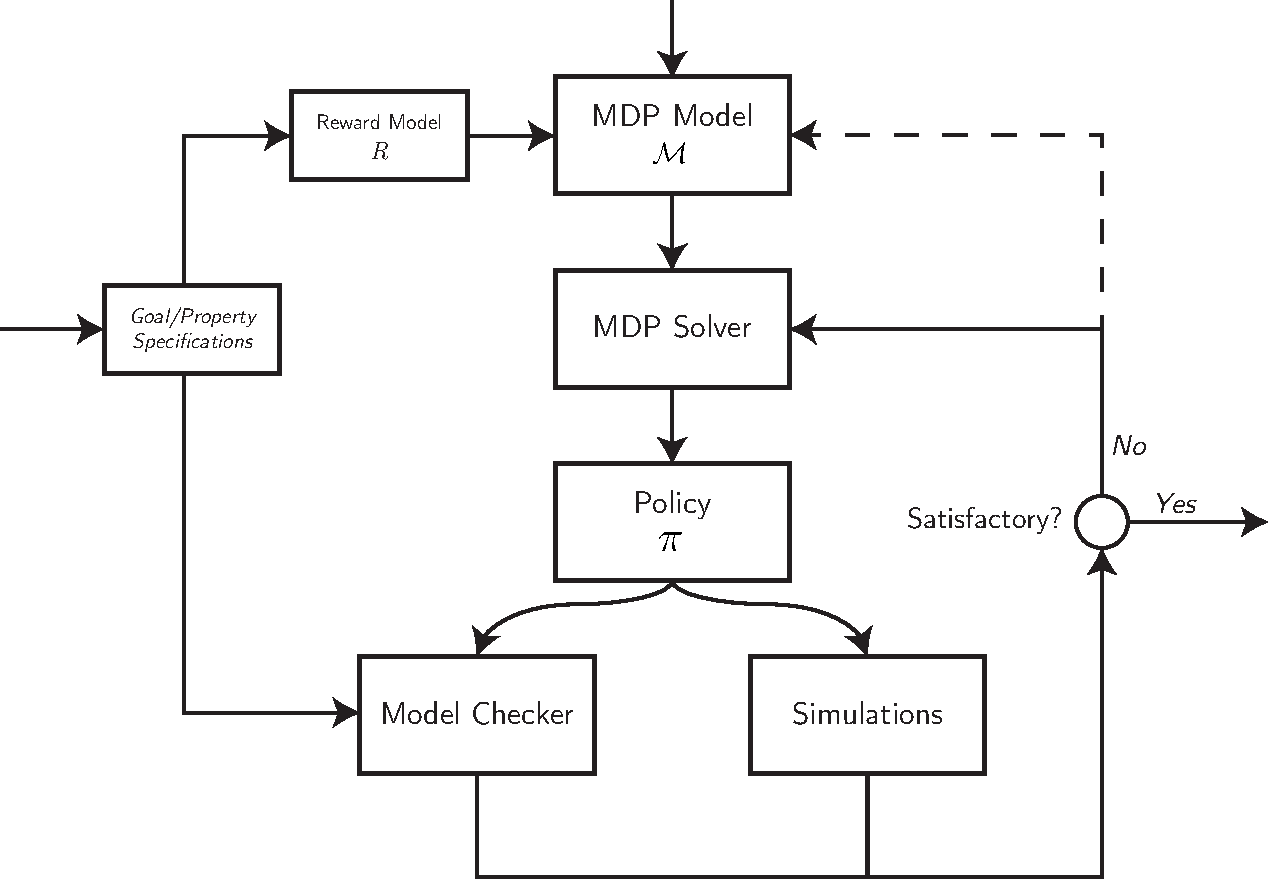
\includegraphics[width=\textwidth]{mdp-planning-diagram}
	\caption{Block diagram of the embedded system's overall software architecture.}
	\label{fig:architecture}
\end{figure}
% Planning algorithms for MDPs
% Planning algorithms for POMDPs

% 










% perceptual aliasing!!!!!!
%\chapter{Decision-Theoretic Planning}
\label{ch:background}
% Introduction on what is Decision-Theoretic Planning
Automated \acrfull{acr:sdm} comprises the central problem of planning under uncertainty. 
\acrfull{acr:dtp} is concerned with the design of plans or \textit{policies} for settings in which uncertainty exists about the effects of actions, where the decision maker or \textit{agent} has incomplete information about the environment and its initial conditions, and where trade-offs need to be made between potentially conflicting objectives to determine an optimal course of action.
This chapter gives an introduction to the type of problems faced in \acrshort{acr:dtp} and explains how specialized probabilistic models can be used to solve these problems efficiently.
First of all, in \autoref{sec:problem-formulation} the goal of \acrshort{acr:dtp} and how the problems that are considered are generally approached is discussed.
Subsequently, \autoref{sec:system-representation} gives an overview of the probabilistic models that are used to make the structure of problems in \acrshort{acr:dtp} explicit.
Finally, in \autoref{sec:planning} some of the most common algorithmic planning techniques are discussed, which either learn a plan directly or through learning and solving a model.

\section{General Problem Formulation}
\label{sec:problem-formulation}
% Formulation of what kind of planning problems are considered in Decision-Theoretic Planning

The class of problems that are considered in \acrlong{acr:dtp} are those that require optimal stochastic control through the actions of decision maker(s), referred to as \textit{agent(s)}, in systems whose dynamics can be modeled as \textit{stochastic processes} \cite{Boutilier1999}.
The agent(s) in these systems sequentially need to choose from a set of actions that influence the system's behavior, consequently making the system switch from one state to another.
In these settings the system's current state and the agent's choice of action determines the probability distribution over the states the system might reach next.
In addition, the agent(s) might be uncertain about the system's current state, implying the need to infer from observations and making decisions based on probabilistic estimates of the system's state.

Typically the problems under consideration involve certain objectives to be achieved (e.g., tasks to be fulfilled) or properties to be satisfied (e.g., avoiding certain system states). 
Therefore the agent should decide on a optimal plan or \textit{policy} which makes it most likely for the system to reach its targets, while minimizing the risk of producing undesirable states and the accompanied costs of the policy.
To find such a policy for \acrlong{acr:sdm} problems, a typical approach is to first setup a probabilistic model of the system and then apply a \acrshort{acr:dtp} algorithm on this model.
This probabilistic model comprises a system representation which defines the state space in terms of a set of multi-valued features, the set of actions the agent may select together with the associated uncertainty defined by transition-probabilities, and a goal specification or performance metric typically expressed by means of a reward structure.

Overall \acrshort{acr:dtp} aims to devise planning algorithms for planning under uncertainty, a problem that is addressed in numerous different fields of research such as AI planning and control theory.
In particular difficulties arise when planning techniques are applied to determine courses of action for real-world settings, such as motion or path planning in robotics which both involve the possibility of action failures and disturbances caused by exogenous events.

\section{System Representations: Markov Models}
\label{sec:system-representation}
% Definitions of Markov Models relevant as probabilistic models for planning under uncertainty

As the class of problems considered in \acrshort{acr:dtp} oft to present considerable structure, there exist various proposed solutions for planning under uncertainty that apply model-based approaches.
This type of decision-theoretic planner uses a stochastic model of the environment in which the agent operates, which compasses the uncertainty that is associated with the agent's actions, observations and the exogenous events that might occur.
Typically the uncertainty is modeled by establishing a \textit{state space} for the system accompanied by a set of possible \textit{transitions} between the states that might be induced with a certain probability by an agent executing \textit{actions}.
The most common types of stochastic models that are used in \acrshort{acr:dtp} are called \textit{Markov Models} (sometimes also referred to as \textit{Markovian Models}), which has been motivated by their success in other fields such as speech recognition \cite{baker1992large, gales2008application, rabiner1989tutorial} and \acrfull{acr:rl} techniques \cite{Brafman2002}.
A Markov Model is a stochastic model in which the future states only depend on a limited number of prior observations. In fact, mostly processes or systems are modeled by Markov Models that satisfy the \textit{Markov Property}, which means that the state transitions are independent of any previous states or agent actions.

In the remainder of this section the most common types of discrete-state Markov Models are discussed one by one, starting from the fundamental models known as \textit{Markov Chains} in \autoref{subsec:markov-chains}, followed by their extension of \textit{\acrfullpl{acr:hmm}} in \autoref{subsec:hidden-markov-models}.
This again is followed by a discussion of the discrete-state Markov Models most relevant in \acrshort{acr:dtp}, being \textit{\acrfullpl{acr:mdp}} in \autoref{subsec:mdps} and their extension of \textit{\acrfullpl{acr:pomdp}} in \autoref{subsec:pomdps}.
Finally in \autoref{subsec:other-markov-models} other related state space models are briefly discussed.

\subsection{Markov Chains}
\label{subsec:markov-chains}
% Markov Chains: States and Transitions

The evolution of system or processes can be viewed as so-called \textit{time-series}, in which a set of data-points can be ordered using an underlying physical dimension, typically time \cite{barberBRML2012}.
Formally, time-series can be defined as a series $x_{a:b}$ of data-points, with $x_{a:b} \equiv x_a, x_{a+1}, \ldots, x_b$.
By means of these time-series, probabilistic models can be devised for real-world systems or processes, by introducing the notion of \textit{states} as a description of the system at a particular point in time or \textit{stage}.

On the basis of the class of Markov Models lies the simplifying assumption that each state is only dependent on a limited number of previous states.
Under this assumption a \textit{Markov Chain} (or \textit{Markov Process}) can be defined as a model of a series $q_{1:T}$ of transitions between states $q_i$ drawn from a state space $\mathcal{S} = \{s_1,\ldots,s_n\}$. The initial state $q_1$ of a Markov Chain typically is either fixed or drawn from $\mathcal{S}$ using a probability distribution over initial states.
For the states or variables of a Markov Chain, the earlier mentioned assumption implies the following conditional independence to hold:
\begin{equation}
	p(q_t \vert q_1,\ldots,q_{t-1}) = p(q_t \vert q_{t - L}, \ldots, q_{t-1})
\end{equation}
where $L$ is the so-called \textit{order} of the Markov Chain.
% See summary barberBRML2012

\begin{figure}[t!]
	\captionsetup[subfigure]{justification=centering}
	\centering
	\subcaptionbox{First-order Markov Chain.\label{fig:markov-chains-first-order}}{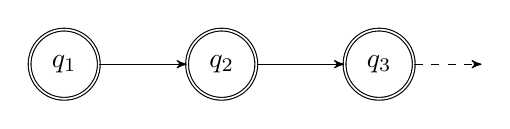
\begin{tikzpicture}[->,>=stealth',auto,node distance=2cm]
		\tikzstyle{every state}=[fill=white,draw=black,text=black,scale=1,double]	% thick
		\node[state] (s1) {$q_1$};
		\node[state] (s2) [right of=s1] {$q_2$};
		\node[state] (s3) [right of=s2] {$q_3$};
		\coordinate (con) at (0,2);
		\path
		(s1)
		edge node {} (s2)
		(s2)
		edge node {} (s3)
		(s3);
		\draw [->, dashed, shorten >=0pt] (s3) to[right] node[auto] {} ++(1.3,0)
		;
		\end{tikzpicture}} \quad
		\subcaptionbox{Second-order Markov Chain.\label{fig:markov-chains-second-order}}{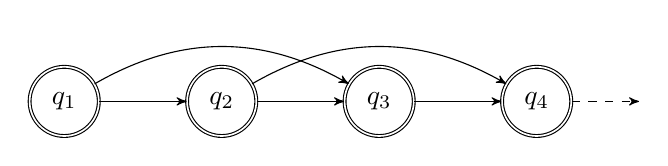
\begin{tikzpicture}[->,>=stealth',auto,node distance=2cm]
		\tikzstyle{every state}=[fill=white,draw=black,text=black,scale=1,double]	% thick
		\node[state] (s1) {$q_1$};
		\node[state] (s2) [right of=s1] {$q_2$};
		\node[state] (s3) [right of=s2] {$q_3$};
		\node[state] (s4) [right of=s3] {$q_4$};
		\path
		(s1)
		edge node {} (s2)
		(s2)
		edge node {} (s3)
		(s1)
		edge [bend left] node {} (s3)
		(s3)
		edge node {} (s4)
		(s2)
		edge [bend left] node {} (s4)
		;
		\draw [->, dashed, shorten >=0pt] (s4) to[right] node[auto] {} ++(1.3,0)
		;
		\end{tikzpicture}}
	\caption{Graphical representation of different types of Markov Chains.}
	\label{fig:markov-chains}
\end{figure}

As depicted in \autoref{fig:markov-chains}, Markov Chains of different order can be defined. \autoref{fig:markov-chains-first-order} exemplifying a first-order Markov Chain in which each state only depends on the previous state, and \autoref{fig:markov-chains-second-order} showing a second-order Markov Chain in which each state depends on the two prior states of the Markov Chain.
In the special case where the transition distribution is independent of the stage of the system, but solely on the prior state(s), one speaks of a \textit{stationary} or \textit{homogeneous} Markov Chain.

Though, mostly first-order Markov Chains as depicted in \autoref{fig:markov-chains-first-order}, which are said to satisfy the \textit{Markov Property}, are applied widely for modeling stochastic processes, such as physical phenomena and economic time-series \cite{bacciu2015probabilistic}.
In addition, mostly compact, stationary, discrete-time, finite-space Markov Chains are used, bearing in mind the computational adequacy of the model (i.e., the larger the state space and order, the more computational cost might be incurred).
Some concrete examples of practical applications include assessing the reliability and/or safety of appliances in engineering \cite{cochran2001generic, cronvall2009combining,el2008optimal}, modeling water flows \cite{parent1991stochastic}, or modeling loan defaults \cite{grimshaw2011markov} in the financial world (for an overview see \cite{pasanisi2012estimating}).

In these chains the state transition probabilities can be stored in an $n \times n$ transition matrix $\mat{A} = [a_{ij}]$ with each entry
\begin{equation}
	a_{ij} = p(q_{t+1} = s_i\vert q_t = s_j)
\end{equation}
denoting the probability of state $s_i$ following state $s_j$.
Similarly, the initial state probabilities can be recorded in an $n \times 1$ initial state vector $\arr{\pi} = [\pi_i]$ with each entry
\begin{equation}
	\pi_i = p(q_1 = s_i)
\end{equation} 
denoting the probability of state $s_i$ being the initial state of the model.
Putting these components all together, a discrete stationary first-order Markov Chain can be defined as a 3-tuple $\mathcal{M} = (\mathcal{S}, \mat{A}, \arr{\pi})$ with $\mathcal{S}$ as state space, $\mat{A}$ as transition matrix and $\arr{\pi}$ as initial state vector.

\subsubsection*{Fitting Markov Chains}
There exist efficient methods for fitting a discrete stationary first-order Markov Chain provided a collected dataset describing the evolution of a stochastic process either by applying likelihood maximization (e.g., see \cite{bacciu2015probabilistic, barberBRML2012, lee1968maximum, teodorescu2009maximum}) or Bayesian inference (e.g., see \cite{barberBRML2012, lee1968maximum, minka2003bayesian}).
These methods estimate the transition distribution to fit a Markov Chain on a collected sequence of time-ordered states. 

The first-mentioned approach of likelihood maximization, works by estimating the transition probabilities by counting the observed transitions in the state sequence.
That is, if we let $n_{ij}$ denote the number of observed transitions from state $s_j$ to state $s_i$, then the maximum-likelihood estimation of the corresponding transition probability is
\begin{equation}
	p(q_{t+1} = s_i\vert q_t = s_j) = \frac{n_{ij}}{\sum_j n_{ij}}
\end{equation}

The second-mentioned approach of Bayesian inference is more suitable for many real-life problems, for which state sequences are incomplete, i.e. states are recorded only for certain stages, meaning there might be gaps in-between.
This type of approach aims to make an estimation of the transition probabilities by adopting a prior for the transition matrix $\mat{A}$, a convenient choice being a factorized prior from the product of $n$ independent \textit{Dirichlet} distributions, one for each row $\mat{A}_j$ such that:
\begin{equation}
	p(\mat{A}) = \prod_{j} \text{Dir}(\mat{A}_j \vert \alpha_j)
\end{equation}
parametrized by a vector $\arr{\alpha}$ with $\alpha_j > 0$ \cite{pasanisi2012estimating,barberBRML2012}.

\subsection{Hidden Markov Models}
\label{subsec:hidden-markov-models}
% Hidden Markov Models: Observations (partially observable) 
% also called latent
% inference problems
% shortly discuss the succesful applications see \cite{barberBRML2012} speech recognition, object tracking, genetic sequence analysis and add citations to the corresponding works

The Markov Chain model discussed in \autoref{subsec:markov-chains} requires the modeled system or stochastic process to be fully observable, meaning that each of its states correspond directly to an observation.
However, it is not unusual to encounter real-world systems in which the states are assumed to be unobservable, though are correlated with observable events produced by the system.
These systems can be modeled by a \acrfull{acr:hmm} in which the states, typically referred to as \textit{hidden} or \textit{latent} variables $h_{1:T}$, are unknown.
Additionally this model consists of observations, typically referred to as \textit{observed} or \textit{visible} variables $v_{1:T}$, which are dependent on the hidden variables through an emission $p(o_t\vert h_t)$ graphically depicted in \autoref{fig:hmm}. All by all a stationary \acrshort{acr:hmm}
consists of the following parts:

\begin{itemize}
	\item a discrete set of $n$ attainable states $\mathcal{S} = \{s_1, \ldots, s_n\}$, i.e. the underlying \textit{state space}
	\item a set of $m$ possible observations, $\mathcal{V} = \{v_1, \ldots, v_m\}$, i.e. the \textit{observation space}
	\item an $n \times n$ transition matrix $\mat{A} = [a_{ij}]$ defining the models' \textit{transition distribution} in which $a_{ij} = p(h_{t+1} = s_i \vert h_t = s_j)$ is the probability of state $s_i$ following state $s_j$ ($s_i, s_j \in \mathcal{S}$)
	\item an $m \times n$ emission matrix $\mat{B} = [b_{ij}]$ defining the models' \textit{emission distribution} in which $b_{ij} = p(o_t = v_i \vert h_t = s_j)$ the probability of observing $v_i$ from state $s_j$ ($v_i \in \mathcal{V}$, $s_j \in \mathcal{S}$)
	\item an $n \times 1$ initial state array $\arr{\pi} = [\pi_i]$ in which $\pi_i = p(h_1 = s_i)$ is the probability of having $s_i$ as the initial state ($s_i \in \mathcal{S}$)
\end{itemize}
Putting all of these components together, a stationary \acrshort{acr:hmm} can be defined as a 5-tuple $\mathcal{M} = (\mathcal{S}, \mathcal{V}, \arr{\pi}, \mat{A}, \mat{B})$ with $\mathcal{S}$ as state space, $\mathcal{V}$ as observation space, $\arr{\pi}$ as initial state vector, $\mat{A}$ as transition matrix and $\mat{B}$ as emission matrix.

\begin{figure}[t!]
	\centering
	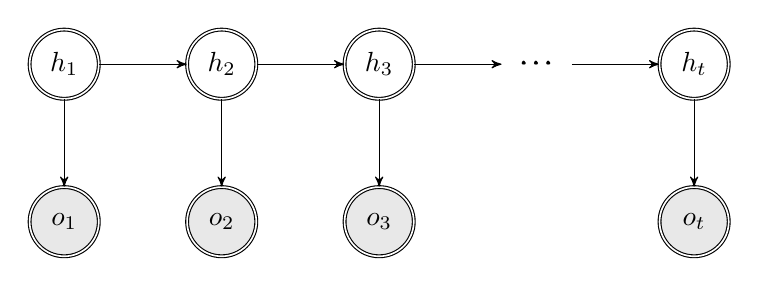
\begin{tikzpicture}[->,>=stealth',auto,node distance=2cm]
	\tikzstyle{every state}=[fill=white,draw=black,text=black,scale=1,double]	% thick
	\node[state] (h1) {$h_1$};
	\node[state] (h2) [right of=h1] {$h_2$};
	\node[state] (h3) [right of=h2] {$h_3$};
	\node[state, draw=none] (dots) [right of=h3] {$\pmb{\cdots}$};
	\node[state] (ht) [right of=dots] {$h_t$};
	\node[state,fill={rgb:black,1;white,10}] (o1) [below of=h1] {$o_1$};
	\node[state,fill={rgb:black,1;white,10}] (o2) [below of=h2] {$o_2$};
	\node[state,fill={rgb:black,1;white,10}] (o3) [below of=h3] {$o_3$};
	\node[state,fill={rgb:black,1;white,10}] (ot) [below of=ht] {$o_t$};
	\path
	(h1)
	edge node {} (h2)
	(h2)
	edge node {} (h3)
	(h3)
	edge node {} (dots)
	(dots)
	edge node {} (ht)
	(h1)
	edge node {} (o1)
	(h2)
	edge node {} (o2)
	(h3)
	edge node {} (o3)
	(ht)
	edge node {} (ot)
	;
	\end{tikzpicture}
	\caption{Graphical representation of an \acrshort{acr:hmm} with hidden states $h_t \in \mathcal{S}$ and observations $o_t \in \mathcal{V}$ for $t = 1:T$}
	\label{fig:hmm}
\end{figure}

In practice \acrshortpl{acr:hmm} have a wide range of applications. One example is that of object tracking in which inference algorithms for \acrshortpl{acr:hmm} are used to estimate the (unknown) position of objects by a sequence of observations \cite{caelli2001shape}. Another well-known application example of \acrshortpl{acr:hmm} is that in automatic speech recognition \cite{}. % TODO Elaborate (_little_ bit) and add citations

% Input figure showing graphical representation of an HMM
% Input subsubsection* about inference problems (see the three in thesis-plan, but also mention the other two)

\subsubsection*{Inference Problems}
The most notable inference problems for \acrshortpl{acr:hmm} are the following: %TODO Little introduction to this section?

\begin{description}
	\item[Evaluation] The \textit{Evaluation} or \textit{Likelihood Problem} is, given an \acrshort{acr:hmm} model $\mathcal{M}$ and an observation sequence $O = (o_1,\ldots,o_T)$ of length $T$, to determine $p(O\vert \mathcal{M})$, which is the likelihood of the observation sequence $O$ being produced by $\mathcal{M}$.
	\item[Optimal States] The \textit{Optimal State Sequence Problem} or \textit{Most Likely Hidden Path Problem} is, given an \acrshort{acr:hmm} model $\mathcal{M}$ and an observation sequence $O = (o_1,\ldots,o_T)$ of length $T$, to determine $H^\ast = \argmax_H p(H \vert O)$, i.e., finding the best state sequence $H^\ast = (h_1^\ast, \ldots, h_T^\ast)$ of length $T$ for the underlying Markov Chain.
	\item[Learning] The \textit{Learning Problem} is, given a set $\mathcal{O} = \{O_1, \ldots, O_k\}$ of independently and identically distributed observation sequences each of length $T$, to find an \acrshort{acr:hmm} $\mathcal{M}^\ast = \argmax_\mathcal{M} p(\mathcal{O}\vert \mathcal{M})$, i.e., maximizing the probability of the model having produced the observation sequences.
\end{description}
Other closely related inference problems are that of \textit{filtering} (inferring the present: $p(h_t\vert o_{1:t})$), \textit{prediction} (inferring the future: $p(h_t \vert o_{1:s})$ with $t > s$) and \textit{smoothing} (inferring the past: $p(h_t \vert o_{1:u})$ with $t < u$).

\subsection{Markov Decision Processes}
\label{subsec:mdps}

% MDPs: Actions --> Is a probabilistic model			% Driven by the actions of an agent
% 	(Exogeneous) events
% Policies

Although Markov Chains and \acrshortpl{acr:hmm} can be used to model the evolution of stochastic processes or systems, they do not allow for stochastic control through the actions of a decision maker or \textit{agent} which alter the state of the system.
The systems of interest in \acrshort{acr:dtp} however, involve agents that are assigned the task of influencing the behavior of the stochastic system by making sequential decisions to achieve certain goals.

% Actions
\acrfullpl{acr:mdp} extend on (stationary) Markov Chains by adding a finite set of actions $A$ available to the agent at each stage or \textit{decision epoch}.
Upon the agent choosing to perform an action $a \in A$, a state transition occurs in response to the action.
However, due to the uncertainty in the system, the actual transition that occurs might differ from the transition intended by the chosen action.
This uncertainty is captured by defining a probabilistic transition function $\delta: \mathcal{S} \times A \times \mathcal{S} \mapsto [0,1]$ which maps the combination of a current state and action to a probability of ending up in a certain next state.

% Reward structure
As the agent of an \acrshort{acr:mdp} aims to fulfill certain goals through the selection of actions, it requires some means of assessing which action is the best to pick.
The value measure used in \acrshortpl{acr:mdp} is defined by a mapping $R: \mathcal{S} \times A \times \mathcal{S} \mapsto \mathbb{R}$ from states and actions to real-valued \textit{rewards} (in case of added value) and/or \textit{costs} (in case of lost value).
Due to the uncertainty in the modeled system, typically the agent uses the \acrshort{acr:mdp}'s transition distribution (defined by transition function $\delta$) to compute expected values, and accordingly selects actions that maximize this quantity.

% Formal definition
Putting all of these components together, an \acrshort{acr:mdp} can be defined as a 5-tuple, $\mathcal{M} = (\mathcal{S}, s_0, A, \delta, R)$ with $\mathcal{S}$ as state space, $s_0 \in \mathcal{S}$ as the initial state, $A$ as finite set of possible actions, $\delta$ as probabilistic transition function and $R$ as reward function.

% Policies
In the context of \acrshort{acr:dtp}, \acrshortpl{acr:mdp} are used to find an optimal course of action, often referred to as a plan or \textit{policy}.
For an \acrshort{acr:mdp} the optimal policy typically means the policy that when applied by an agent, maximizes the expected value.
Although, one can also choose to express goals in alternative ways that does not require the specification of a reward function.
An example of this can be seen in \cite{bhatia2010sampling, lacerda2015optimal}, which replaces the reward function of the classic MDP-framework by a (co-safe) Linear Temporal Logic (LTL) formula to be satisfied.

\subsection{Partially Observable MDPs}
\label{subsec:pomdps}

% Observations: .. POMDP
% Reward Models and Value Functions

An extension of the traditional \acrshort{acr:mdp} models, are the \acrfull{acr:pomdp} models which account for uncertainty in the observations that are made by agents.
That is, while an \acrshort{acr:mdp} is used to model systems that are fully observable, in a \acrshort{acr:pomdp} the states are not observable and can only be inferred from the observations that are perceived.
In other words, we can intuitively view a \acrshort{acr:pomdp} as the combination of a \acrshort{acr:hmm} and an \acrshort{acr:mdp}.

As such, a \acrshort{acr:pomdp} can be defined as a 7-tuple $\mathcal{M} = (\mathcal{S}, s_0, A, \delta, \mathcal{O}, \Omega, R)$ with $\mathcal{S}$ as state space, $s_0 \in \mathcal{S}$ as the initial state, $A$ as finite set of possible actions, $\delta$ the transition function, $\mathcal{O}$ the observation space, $\Omega$ an emission or observation probability function and $R$ as reward function.
As the true state of a \acrshort{acr:pomdp} is unknown, the transition function $\delta$ is defined over beliefs of states, and accordingly a policy $\pi$ maps beliefs to actions.
The observation function $\Omega: \mathcal{S}\times A \mapsto \mathcal{O}$ defines the probability of observations from state-action pairs in the \acrshort{acr:pomdp} and is used to iteratively update the belief-state of an agent.

\subsection{Other Markov Models and Related State-Space Models}
\label{subsec:other-markov-models}
Apart from the discrete-state Markov Models that were discussed in this section, there exist numerous other types of Markov Models and closely related State-Space Models (SMMs), including among others the following:%, including continuous-state Markov Models (e.g., Linear Dynamical Systems with a Gaussian state-space \cite{Minka1999,barberBRML2012}) and other specialized variations. 

\begin{description}
	\item[Factored Markov Decision Process (FMDP)] An extension of the MDP model that allows for compact representation of states, transitions and rewards \cite{Degris2010}. In many real-life domains especially the state-space grows exponentially with the number of variables. Therefore FMDPs can be used to exponentially reduce the representation by means of a dynamic Bayesian network. The main drawback, however, is that finding the best policy becomes an NP-hard problem.
	\item[Multi-Agent \acrshort{acr:mdp} (MMDP)] An \acrshort{acr:mdp} model for systems that involve multiple decision makers. In this model each agent chooses an individual action with the goal of optimizing a joint reward. Other variations involving multiple agents are Decentralized \acrshortpl{acr:mdp} (Dec-MDPs) and \acrshortpl{acr:pomdp} (Dec-POMDPs), which differ from MMDPs in that the agents can only approximate the global state of the process by their own (local) observations \cite{Melo20111757}.
	%\item[Variable-order Markov Model (VOM)] To be determined 
	\item[Linear Dynamical System (LDS)] A continuous-state State-Space Model with linear dynamics, Gaussian state space and the assumption of hidden variables as in \acrshortpl{acr:hmm} \cite{Minka1999, barberBRML2012, Ghahramani2000}.
\end{description}
% TODO Extend each with sentence to explain the need for these models

As the remaining chapters only consider systems and processes that are modeled using discrete-state Markov Models, these variations will not be further discussed in more detail.

\section{Learning Optimal Policies}
\label{sec:planning}

In \acrshort{acr:sdm} problems typically the aim is to determine a policy that maximizes the total expected value obtained.
In algorithmic planning techniques a probabilistic model of the environment, which includes estimates of the transition probabilities and rewards, is used to obtain an optimal policy by exploring its state-space towards a goal.
On the other hand, in \acrfull{acr:rl} the optimal policy is learned while interacting with the environment and it is applied when one does not know the transition probabilities and rewards for its states upfront.
Both techniques have in common that they iteratively update estimations of a value function to derive a policy.
The main difference though is that in planning this progress is carried out based on simulated experience from a model, while in learning techniques this is based on real experience from executing agents in an environment \cite{sutton1998reinforcement}.
So, even when considering the differences, various solutions can be exchanged between planning and \acrshort{acr:rl} techniques.

In this section the various approaches for finding optimal policies are discussed, where the planning techniques are discussed in \autoref{subsec:model-based-planning}, and \acrshort{acr:rl} techniques are discussed in \autoref{subsec:reinforcement-learning}.

% Sutton and Barto (1998/2012) describe two approaches for rl solutions when the transition and reward functions are not known	(Learning the Structure of Factored Markov Decision Processes inReinforcement Learning Problems)
% See chapter 8.2, show an adapted version of the figure and explain advantages and disadvantages
% Explain the difference between planning and learning

\begin{figure}[t!]
	\centering
	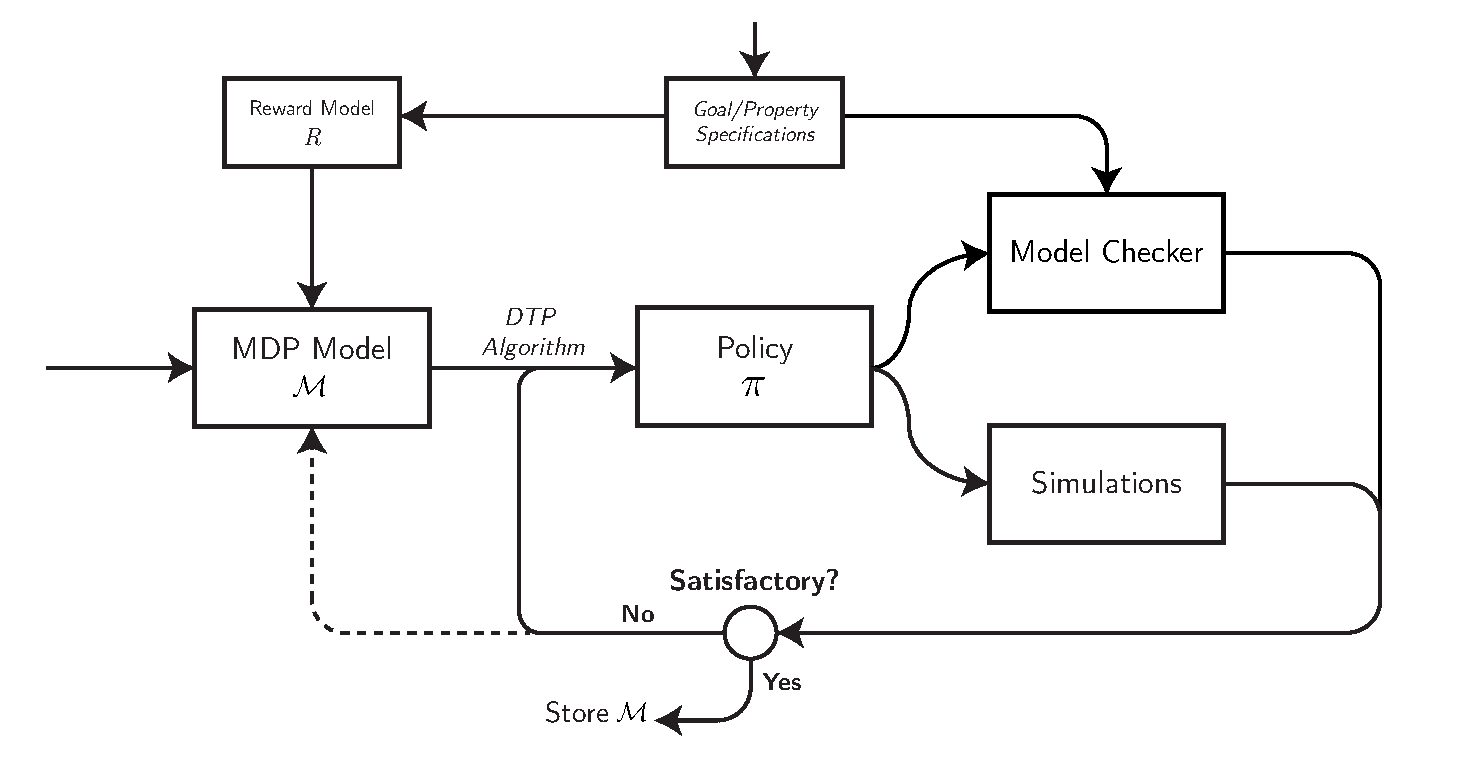
\includegraphics[width=\textwidth]{mdp-planning-diagram-v2}
	\caption{Block diagram of the generic routine employed in model-based MDP planning techniques.}
	\label{fig:model-based-routine}
\end{figure}

\subsection{Model-Based Planning Techniques}	% Also referred to as Indirect approaches
\label{subsec:model-based-planning}

In \acrshort{acr:dtp} the algorithms compute their plans or policies based on a probabilistic model of the environment.
Most common is to prepare an \acrshort{acr:mdp} and apply exact dynamic programming solutions to compute an optimal policy for that model.
The routine that is typically followed in MDP planning is depicted in \autoref{fig:model-based-routine}.
The state space, transition function and action space are usually handcrafted, based on expertise or trial and error.
The goal that should be fulfilled is translated into a reward model, mapping positive highly-valued rewards to desirable states and low rewards or costs to states that are not desirable or should even be avoided.
These parts together form the \acrshort{acr:mdp} which is fed to a planning algorithm which in this case is referred to as \textit{\acrshort{acr:mdp} solver}.
From this solver, a policy $\pi$ is obtained, which is usually evaluated by applying it in one or more simulations, rather than using it in a real-world environment.
Another option is to make use of automated model checking tools which can verify whether the policy will satisfy the set goals. % TODO Add citation to book about model checking from APS and Bruno
After evaluating the current policy, one may choose to stick with the current policy or adjust the settings of the solver or \acrshort{acr:mdp} model and obtain a new policy.

There are several options for the \acrshort{acr:mdp} solver, which compute an optimal policy by maximization of the expected value to be obtained.
In the remainder of this section various of these planning algorithms for \acrshortpl{acr:mdp} are discussed and evaluated.

\begin{algorithm}[]
	\caption{Value iteration}
	\label{alg:vi}
	\begin{algorithmic}[1]
		\Require{MDP $\mathcal{M} = (\mathcal{S}, s_0, A, \delta, R)$, discount factor $\gamma \in (0, 1)$, threshold $\xi > 0$}
		\Ensure{Optimal policy $\arr{\pi}^*: \mathcal{S} \mapsto A$}
		\State{Initialize $V_t: \mathcal{S} \mapsto \mathbb{R}$ arbitrarily for $t = 0$}
		\State $t \gets 0$
		\Repeat
		\State $t \gets t + 1$
		\ForAll{$s \in \mathcal{S}$}
		\State{$V_t(s) \gets \max_{a \in A} \left[\sum_{s' \in \mathcal{S}} \delta(s, a, s') \cdot \left[R(s, a, s') + \gamma \cdot V_{t-1}(s')\right]\right]$}
		\EndFor
		\Until{$\forall s \in \mathcal{S}: \lvert V_t(s) - V_{t-1}(s) \rvert \leq \xi$}
		\ForAll{$s \in \mathcal{S}$}
		\State $\arr{\pi}^*(s) \gets \text{arg max}_{a \in A} \left[\sum_{s' \in \mathcal{S}} \delta(s, a, s') \cdot \left[R(s, a, s') + \gamma \cdot V_{t}(s')\right]\right]$
		\EndFor
		\State\Return $\arr{\pi}^*$
	\end{algorithmic}
\end{algorithm}

\subsubsection*{Value Iteration}
\label{sec:value-iteration}

The most well-known algorithm for obtaining optimal policies from \acrshortpl{acr:mdp} is \textit{\acrfull{acr:vi}}, which is a synchronous dynamic programming solution which iteratively updates a value function $V: \mathcal{S} \mapsto \mathbb{R}$ until convergence given an MDP model $\mathcal{M} = (\mathcal{S}, s_0, A, \delta, R)$.
The updates are performed through so-called \textit{Bellman backups} based on the following Bellman equation:
\begin{align}
	V^*(s) &= max_{a \in A} \left[\sum_{s' \in \mathcal{S}} P(s' \vert s, a) \cdot \left[R(s, a, s') + \gamma \cdot V^*_{t}(s')\right]\right]	&\forall s \in \mathcal{S}
\end{align}
where $\gamma \in (0,1)$ is a discount factor which expresses the magnitude of preference of short-term solutions over long-term solutions. That is, the smaller the factor $\gamma$, the more important it is that goals are reached in as few steps as possible.

In \autoref{alg:vi}, it is shown how the \acrshort{acr:vi} algorithm can be used to obtain optimal policies for an MDP (based on the formulation in \cite{poole2010artificial}).
Intuitively, \acrshort{acr:vi} can be viewed as estimating the values starting from the goal-rewards and working backwards.
The initial values of the value function, stored in $V_0$, can be arbitrarily initialized, but to achieve faster convergence it is customary to do the initialization based on a rough estimation of $V^*$.
In every iteration, the estimates of the value function are updated by the backup operations based on the value in previous operations.
After a finite number of iterations the algorithm will converge (as is shown in \cite{puterman2014markov}) and after that point $V(s)$ gives us the maximum to be expected sum of rewards starting from a state $s \in \mathcal{S}$.
As can be seen in \autoref{alg:vi}, convergence is reached as soon as the change in value gets below a given threshold $\xi > 0$.
After such convergence has been reached, the policy can be defined by selecting the action $a \in A$ for each state $s \in \mathcal{S}$ that is most likely to maximize the collected rewards based on the value of $V_t(s)$.
All by all, the algorithm works well when the state space is relatively small, but for large state spaces more storage is required and it may take longer to reach convergence.

Note that an alternative formulation of the \acrshort{acr:vi} algorithm can be given that makes use of a $Q$-table instead of a value-function $V$.
In this formulation the entries $Q(s, a)$ are updated in each iteration for each state-action pair.
The optimal policy can then be obtained directly by selecting the action with the maximum value in the $Q$-table for each action, though it requires more storage compared to a value function.\newpage

\subsubsection{Asynchronous Value Iteration}
\label{sec:gs-value-iteration}

An adaptation of the traditional \acrshort{acr:vi} algorithm is \textit{asynchronous \acrshort{acr:vi}}, which is an asynchronous dynamic programming solution.
Almost all of the steps in asynchronous \acrshort{acr:vi} are the same except that rather than updating the value function $V: \mathcal{S} \mapsto \mathbb{R}$ for each state in each iteration, the function is updated only for a single state in each iteration in no particular order (or even randomized).
In the case of a fixed ordering, this algorithm is usually referred to as \textit{Gauss-Seidel \acrshort{acr:vi}}.
Compared to the traditional \acrshort{acr:vi} algorithm, the asynchronous adaptation requires less space and converges faster, especially when updates occur more often for most relevant states and the update ordering is adjusted carefully.

\textit{\acrfull{acr:rtdp}} \cite{barto1995learning} is a family of asynchronous \acrshort{acr:vi} algorithms which aim to find policies by performing updates and concurrently controlling the \acrshort{acr:mdp} (based on the policy corresponding to the latest estimate of the value function).
Opposed to traditional \acrshort{acr:vi}, where solving \acrshortpl{acr:mdp} with large state spaces is infeasible, RTDP algorithms often converge without examining all states.

% TODO POMDP Adaptation of Value Iteration See AI: A Modern Approach + Probabilistic Robotics

\begin{algorithm}[]
	\caption{Policy iteration}
	\label{alg:pi}
	\begin{algorithmic}[1]
		\Require{MDP $\mathcal{M} = (\mathcal{S}, s_0, A, \delta, R)$, discount factor $\gamma \in (0, 1)$}
		\Ensure{Optimal policy $\arr{\pi}^*: \mathcal{S} \mapsto A$}
		\State{Initialize $\arr{\pi}_0$}
		\State $t \gets 0$
		\Repeat
		\State Solve $\forall s \in \mathcal{S}$: $V_{\arr{\pi}_{t}}(s) \gets \sum_{s' \in \mathcal{S}} \delta(s, \arr{\pi}_t(s), s') \cdot \left[R(s, \arr{\pi}_t(s), s') + \gamma \cdot V_{\arr{\pi}_{t}}(s')\right]$
		\State $t \gets t + 1$
		\ForAll{$s \in \mathcal{S}$}
		\State $\arr{\pi}_t(s) \gets \argmax_{a \in A} \left[\sum_{s' \in \mathcal{S}} \delta(s, a, s') \cdot \left[R(s, a, s') + \gamma \cdot V_{\arr{\pi}_{t - 1}}(s')\right]\right]$
		\EndFor
		\Until{$\arr{\pi}_{t} = \arr{\pi}_{t-1}$}
		\State\Return $\arr{\pi}_t$
	\end{algorithmic}
\end{algorithm}

\subsubsection{Policy Iteration}
\label{sec:policy-iteration}

Another algorithm that is widely applied for obtaining policies from \acrshortpl{acr:mdp} is known as \textit{\acrfull{acr:pi}}. As shown in \autoref{alg:pi} \acrshort{acr:pi} starts off with an initial policy vector $\arr{\pi}_0$ which may be arbitrarily initialized, but preferably by an approximation of an optimal policy for the input MDP $\mathcal{M} = (\mathcal{S}, s_0, A, \delta, R)$ to achieve faster convergence.
Then in each iteration, first the value for each state is computed based on the latest policy $\arr{\pi}_t$, which comes down to solving a set of linear equations.
Solving this set of linear equations can be done by linear programming in (at most) $O(\lvert\mathcal{S}\rvert^3)$ time \cite{littman1995complexity}. 
An alternative approach, known as \textit{modified policy iteration}, is to solve these by applying a simplified form of value iteration in which the actions to select are already known for each state from the policy (i.e., $\arr{\pi}_t(s)$ for each $s \in \mathcal{S}$).
This step which is known as \textit{policy evaluation} is followed by a \textit{policy improvement} step in which the policy is greedily updated based on the latest value function $V_{\arr{\pi}}$.
This process is repeated until no improvements are possible and the policy stops changing.

Compared to \acrshort{acr:vi} the algorithm always converges in a finite number of iterations. However, solving the set of linear equations in each iteration is a more time-costly operation, especially for large state spaces.
That is, in \acrshort{acr:vi} each iteration takes $O(\lvert\mathcal{S}\rvert^2\cdot\lvert A\rvert)$ time, although one must note that the number of iterations is not finite, while \acrshort{acr:pi} finds an optimum in a finite number.\newpage

\begin{algorithm}
	\caption{Backwards induction}
	\label{alg:backwards-induction}
	\begin{algorithmic}[1]
		\Require{MDP $\mathcal{M} = (\mathcal{S}, s_0, A, \delta, R)$, horizon $h \in \mathbb{N}$}
		\Ensure{Optimal policy $\arr{\pi}^*: \mathcal{S} \mapsto A$}
		\State $t \gets h$
		\State $\forall s \in \mathcal{S}: V_h(s) \gets 0$
		\Repeat
		\State $t \gets t - 1$
		\ForAll{$s \in \mathcal{S}$}
		\State $V_t(s) \gets \max_{a \in A} \left[\sum_{s' \in \mathcal{S}} \delta(s,a,s') \cdot \left[R(s,a,s') + V_{t+1}(s')\right]\right]$
		\EndFor
		\Until{$t = 1$}
		\ForAll{$s \in \mathcal{S}$}
		\State $\arr{\pi}^*(s) \gets \argmax_{a \in A} \left[\sum_{s' \in \mathcal{S}} \delta(s,a,s') \cdot \left[R(s,a,s') + V_{1}(s')\right]\right]$
		\EndFor
		\State\Return $\arr{\pi}^*$
	\end{algorithmic}
\end{algorithm}

\subsubsection{Backwards Induction}
\label{sec:backwards-induction}

In the special case of a finite horizon \acrshort{acr:mdp} it is possible to obtain an optimal policy by applying \textit{backwards induction} \cite{chamie2015finite} shown in \autoref{alg:backwards-induction}.
As the name suggests the algorithm works backwards, starting from the last step $h$ and recursively using the value function of step $t + 1$ to compute that of step $t$.
Even though the algorithm works well when dealing with finite horizons, typically real world scenarios more often deal with infinite horizons for planning under uncertainty.

\subsubsection{Linear Programming}
\label{sec:linear-programming}

A less frequently applied approach is that of formulating the \acrshort{acr:mdp} as a \acrfull{acr:lp} and solving it using so-called \textit{simplex} methods.
Following this approach, an \acrshort{acr:lp} formulation for an MDP $\mathcal{M} = (\mathcal{S}, s_0, A, \delta, R)$, as explained in \cite{pazis2012non}, is:

%\begin{align}
%\max_{\lambda} &\sum_{s \in \mathcal{S}}\sum_{a \in A}\sum_{s' \in \mathcal{S}} \lambda(s, a) \delta(s, a, s')R(s, a, s') &\nonumber\\
%\text{s.t.} &\sum_{a' \in A} \lambda(s', a') = \mu_0(s) + \gamma \sum_{s \in \mathcal{S}}\sum_{a \in A} \lambda(s,a)\delta(s,a,s')	&\forall s' \in \mathcal{S} \\
%&\lambda(s,a) \geq 0 &\forall s \in \mathcal{S}, \forall a \in A \nonumber
%\end{align}
\begin{align}
\min_{V} &\sum_{s' \in \mathcal{S}} \mu_0(s) \cdot V(s) &\nonumber\\
\text{s.t. } &V(s) \geq \sum_{s' \in \mathcal{S}} \delta(s, a, s') \left[R(s,a,s') + \gamma\cdot V(s')\right]	&\forall s \in \mathcal{S}, \forall a \in A
\end{align}
where $\mu_0: \mathcal{S} \mapsto [0,1]$ is a probability distribution over the states.

From the solution $V^*$ of this \acrshort{acr:lp} formulation, a policy $\arr{\pi}^*$ can be obtained by letting $\arr{\pi}^*(s) = \argmax_{a \in A} \sum_{s' \in \mathcal{S}} \delta(s, a, s') \left[R(s,a,s') + \gamma\cdot V(s')\right]$ for each state $s \in \mathcal{S}$. This primal formulation optimizes a value function $V$, but alternatively the policy can be optimized directly by considering the dual formulation (see \cite{littman1995complexity}).
Comparing \acrshort{acr:lp} solutions to the specialized \acrshort{acr:vi} and \acrshort{acr:pi} solutions, the latter typically hold more promise for efficient solutions than general-purpose \acrshort{acr:lp} algorithms, although the \acrshort{acr:lp} scale better to larger \acrshort{acr:mdp} planning problems.

\subsection{Reinforcement Learning Techniques}
\label{subsec:reinforcement-learning}

\acrfull{acr:rl} techniques work on real experience based on which they update the behavior of the agent that is defined by an action-selection policy. To do this they require direct interaction with the environment to obtain experience and update value function estimations accordingly during execution.
Although most planning algorithms cannot be used for learning problems, learning algorithms can be used for planning problems as they can make use of simulated experience.
There are several techniques that exist, of which the most common ones are discussed in the remainder of this section.

\newpage

\subsubsection{Q-Learning}
\label{sec:q-learning}

Q-Learning is a model-free reinforcement learning technique which discovers an action-selection policy by learning estimates of the optimal Q-values of an \acrshort{acr:mdp}.
The technique starts off with a Q-table $Q$, which is arbitrarily initialized, containing the Q-values $Q(s,a)$ for each state-action pair $(s,a)$.
In each point in time, the agent for which the Q-Learning technique is applied, is assumed to be in a certain state $s$, and chooses a next action $a$ to execute based on the current Q-value estimates.
After executing an action the agent ends up in a new state $s'$ and observes a certain reward $r$.
The Q-table is then updated accordingly based on the following update rule:
\[
Q(s, a) = Q(s, a) + \alpha \Big[r + \gamma \max_{a'} Q(s',a') - Q(s, a)\Big]
\]
where $\alpha \in (0,1)$ is the learning rate and $\gamma \in (0, 1)$ the discount factor.
The learning rate expresses the rate at which newly acquired information overrides the old information in the Q-table.
Over time the estimates in the Q-table will improve such that the revenue is maximized.
A near-optimal policy can then be constructed by selecting the action with the highest Q-value from the Q-table for each state.

% 
% Also note that it can be used for planning

\subsubsection{SARSA}
\label{sec:sarsa}

\begin{algorithm}
	\caption{SARSA}
	\label{alg:sarsa}
	\begin{algorithmic}[1]
		\Require{MDP $\mathcal{S}, A, \alpha, \gamma$}
		\Ensure{Optimal policy $\arr{\pi}^*: \mathcal{S} \mapsto A$}
		\State Initialize $Q: \mathcal{S} \times A \mapsto \mathbb{R}$ arbitrarily
		\Repeat
		\State Pick $s \in \mathcal{S}$ arbitrarily
		\State $a \gets \pi[s]$ %TODO
			\Repeat
			\State 
			\Until{$s$ is terminal}
		\Until{$Q$ converged}
		\State\Return $\arr{\pi}^*$
	\end{algorithmic}
\end{algorithm}

Another algorithm, similar to Q-Learning, is known as SARSA.
While Q-Learning is an off-policy method which learns the value of the optimal policy, SARSA is an on-policy method which learns the value of the policy it currently follows in order to iteratively improve this policy.
In each iteration, it takes the action yielded by its policy and observes
%\chapter{Bayesian Optimization}
\label{ch:bayesian-optimization}
This chapter elaborates upon a method known as Bayesian optimization, which is used to automate the process of optimizing the parameters of an unknown objective.
First \autoref{sec:bayesian-optimization-problem} introduces the optimization tasks this method is aimed at and how these are relevant to \acrshort{acr:sdm} problems.
Subsequently, in \autoref{sec:bayesian-optimization-algorithm} the optimization method is formally described.
In \autoref{sec:bayesian-optimization-prior-acquisition} the configurable parts of the method are discussed, considering both advantages and disadvantages of available options.
Finally, in \autoref{sec:bayesian-optimization-applications} a number of applications of Bayesian optimization in the field of planning under uncertainty are discussed, serving as an overview of the method's successes in this field.

% More applications:
%https://www.cs.ox.ac.uk/people/nando.defreitas/publications/BayesOptLoop.pdf

\section{Problem Formulation}
\label{sec:bayesian-optimization-problem}

One of the problems that is faced in the field of optimization is that of maximizing a nonlinear, real valued \textit{objective function} $f: \mathcal{X} \mapsto \mathbb{R}$ on a domain $\mathcal{X} \subset \mathbb{R}^m$ ($m \geq 1$).
Formally, to find a global maximizer $x^\ast \in \mathcal{X}$ for which:
\begin{equation}
	x^\ast = \argmax_{x \in \mathcal{X}} f(x)
\end{equation}
In particular the problem turns out to be a common bottleneck when dealing with an objective function that is unknown and expensive to evaluate in terms of the required computational resources.
As an example, one could think of finding the hyper-parameters for a neural network which maximize the performance, where each single evaluation of a set of parameters requires one to train the neural network and assess the performance on a huge dataset.

Although this problem of optimizing expensive functions can be found in many different contexts, it is foremost a problem in sequential decision theory. 
That is, typically one can only hope to estimate objective functions of \acrshort{acr:sdm} problems in AI planning and reinforcement learning through expensive simulations \cite{Brochu2010, Ghahramani2015}.

A naive approach for optimizing the objective would be to evaluate a set of (random) combinations of parameters and see which parameter-settings seem to give the best results.
This approach however, usually requires expert knowledge and might demand a large number of function evaluations that do not necessarily provide new information about the parameter-space.
The method known as \textit{Bayesian optimization}, described in \autoref{sec:bayesian-optimization-algorithm}, improves on these naive approaches by making predictions about which regions of the parameter-space are expected to give the best results and hence limiting the number of function-evaluations.

\section{Algorithm Description}
\label{sec:bayesian-optimization-algorithm}

\textit{Bayesian optimization} is a powerful method for finding the maximum of a typically unknown, expensive, nonlinear objective function, while aiming to minimize the number of objective function evaluations and avoiding local maxima \cite{Brochu2010}.
This method first requires one to set a prior $p(f)$ over the objective function $f$, representing the belief about the space of plausible objective functions.
Then, the algorithm starts off by gathering a small set of initial sample-observation pairs of samples $x \in \mathcal{X}$ and corresponding objective values $y = f(x) + \varepsilon$.
These pairs are then stored in a set $\mathcal{D}_{1:t} = \{(x_i, y_i) \mid i = 1 \ldots t\}$ (i.e., the \textit{evidence set}) where we let $x_i$ denote the $i$th sample and $y_i = f(x_i) + \varepsilon_i$ the corresponding $i$th observation with noise $\varepsilon_i$.

% Posterior / Surrogate Function
The algorithm then derives a posterior distribution $p(f \vert \mathcal{D}_{1:t})$ which is, according to Bayes' Theorem, said to be proportional to the likelihood $p(\mathcal{D}_{1:t} \vert f)$ and the prior $p(f)$ for the first $t$ gathered observations, s.t.:
\begin{equation}
	p(f \vert \mathcal{D}_{1:t}) \propto p(\mathcal{D}_{1:t} \vert f) \cdot p(f)
\end{equation}
This posterior can be viewed as an estimation of the objective function $f$, referred to as a \textit{surrogate function}.
% It does so by applying Bayes' Theorem, which states that the posterior probability $P(M \vert E)$ of a model $M$ given evidence $E$ is proportional to the likelihood $P(E \vert M)$ of $E$ given $M$

% Acquisition function
To decide on which $x \in \mathcal{X}$ to sample and gather a new observation $f(x)$ from next, a so-called \textit{acquisition function} $u: \mathcal{X} \mapsto \mathbb{R}$ is used, which assigns a certain utility to evaluating $f$ at some particular $x \in \mathcal{X}$ given the evidence set $\mathcal{D}$ at that point.
This acquisition function should be defined such that it captures a correct balance between \textit{exploration} (to sample from areas with high uncertainty) and \textit{exploitation} (to sample from areas likely to improve on prior observations). For this reason many different classes of acquisition functions exist, which are discussed in little more detail in \autoref{sec:bayesian-optimization-prior-acquisition}.

% General Formulation Algorithm

\begin{algorithm}
	\caption{Bayesian Optimization (General Formulation) \label{alg:bayesian-optimization}}
	\begin{algorithmic}[1]
		\Require{Domain $\mathcal{X} \subset \mathbb{R}^m (m \geq 1)$, prior $p(f)$ and acquisition function $u: \mathcal{X} \mapsto \mathbb{R}$}
		\Let{$\mathcal{D}_0$}{$\emptyset$} \Comment{$\mathcal{D}$ is the evidence set}
		\For{$t \gets 1, 2, \ldots$}
			\Let{$x_t$}{$\argmax_{x \in \mathcal{X}} u(x \vert \mathcal{D}_{1:t-1})$} \Comment{Acquisition based on posterior $p(f \vert \mathcal{D}_{1:t})$}%\Comment{Retrieve the next sample}
			\Let{$y_t$}{$f(x_t) + \varepsilon_t$}  %\Comment{Record a new observation of $f$}
			\Let{$\mathcal{D}_{1:t}$}{$\mathcal{D}_{1:t-1} \cup \{(x_t, y_t)\}$} \Comment{Augment $\mathcal{D}$ with the new evidence}
			\State Update the prior $p(f)$ and posterior $p(f \vert \mathcal{D}_{1:t})$
			\State \textit{Break} when satisfactory \Comment{Stop condition defined by implementation}
		\EndFor
		\State \Return{$\argmax_{(x_i, y_i) \in \mathcal{D}} y_i$}
	\end{algorithmic}
\end{algorithm}

The general formulation of the Bayesian Optimization is presented in \autoref{alg:bayesian-optimization}.
For an implementation of the algorithm still three components need to be defined, which are the domain $\mathcal{X}$ of $f$, the prior over $f$, and last of all the acquisition function $u$.

\section{Choice of Prior and Acquisition Function}
\label{sec:bayesian-optimization-prior-acquisition}
In order to apply Bayesian optimization there are two major choices that need to be made, which are those of the prior distribution over the objective and the acquisition function. In this section the different options and corresponding considerations that need to be made for these two components are elaborated upon.

\subsection*{Prior Distributions}
\label{sec:bayesian-optimization-prior}
In Bayesian optimization the most common choice for the prior distribution is a \acrfull{acr:gp}, which is typically well-suited as it accounts for the uncertainty associated with each prediction.
Another important aspect that makes a \acrshort{acr:gp} a convenient choice for the prior distribution is that it induces a posterior distribution over the objective function that is analytically tractable.
Intuitively a \acrshort{acr:gp} can be viewed as a prior which assumes that similar inputs result in similar outputs.
For an objective function $f$, the \acrshort{acr:gp} defines a Gaussian probability distribution over $f(x)$ for each $x$, so that a \acrshort{acr:gp} can be expressed as a probability distribution over functions:
\begin{equation}
	P(f(x) \vert x) = \mathcal{N}(\mu(x), \sigma^2(x))
\end{equation}
where $\mathcal{N}$ denotes a normal distribution, while $\mu$ and $\sigma$ denote mean and standard deviation respectively.
By this definition, a \acrshort{acr:gp} can be viewed as a function that returns the mean and variance of a normal distribution over the possible values of $f$ at $x$. A \acrshort{acr:gp} as prior over an objective function $f$ is typically denoted as: 
\begin{equation}
\label{eq:gp}
f \sim GP(m(\cdot), K(\cdot, \cdot))
\end{equation}
so that the \acrshort{acr:gp} is completely specified by a mean function $m$ and a \textit{kernel} function $K$ defining the covariance.
The mean function $\mu$ is typically initialized by a constant mean, usually zero, due to the assumption that all points in the parameter space are equally likely and because the conditional mean can still be flexibly specified by the kernel function $K$ \cite{kawaguchi2015bayesian}.

The choice of the kernel or covariance function of the \acrshort{acr:gp} determines the smoothness of the estimations on the performance and confidence intervals of unexplored samples in the parameter space.
According to the various literature in the field of Bayesian Optimization the most common kernels are said to be the \textit{squared exponential} (also known as \textit{radial basis function (RBF)} or Gaussian) kernel and Mat\'ern kernel.
However, the squared exponential kernel turns out unrealistically smooth for practical applications \cite{snoek2012practical} and therefore would require properly selecting its hyper-parameters.
The Mat\'ern kernel serves as a more flexible class, where the hyper-parameters allow tweaking the distance at which there are almost no effects from previous samples and the rate at which these effects decrease, for which a reoccurring kernel appears to be an automatic relevance determination (ARD) Mat\'ern 5/2 kernel for machine learning applications \cite{snoek2012practical, kawaguchi2015bayesian}.


%\begin{itemize}
%	\item \acrfull{acr:gp}
%	\item Wiener Process
%\end{itemize}


\subsection*{Acquisition Functions}
\label{sec:bayesian-optimization-acquisition}
% Examples acquisition function: PMAX, IEMAX, MPI, MEI, (GP-)UCB, GP-Hedge
% TODO Introduction
Let us define $f(x^+)$ as the `best' observation, corresponding to the sample $x^+ = \argmax_{x_i \in x_{1:t}} y_i$ when considering the first $t$ samples.

% TODO "Best-known acquisition functions:"
\begin{description}
	\item[\acrfull{acr:mpi}] This acquisition function selects the next sample to maximize the probability of improvement, which is the sample $x \in \mathcal{X}$ so that:
	$$P(f(x) \geq f(x^+) + \xi)$$
	where $\xi \geq 0$ is a trade-off parameter.
	\begin{description}
		\item[Advantages] description
		\item[Disadvantages] description
	\end{description}
	\item[\acrfull{acr:mei}] description
	\begin{description}
		\item[Advantages] description
		\item[Disadvantages] description
	\end{description}
	\item[\acrfull{acr:gp-ucb}] description
	\begin{description}
		\item[Advantages] description
		\item[Disadvantages] description
	\end{description}
\end{description}

Others possible acquisition functions that are used in Bayesian optimization are PMAX, IEMAX and GP-HEDGE. % TODO

\section{Applications of Bayesian Optimization to Planning Problems}
\label{sec:bayesian-optimization-applications}

% TODO Write out completely, this is just a short overview
Most interesting applications that involve or are closely related to \acrshort{acr:dtp}:

In \cite{MartinezCantin2009}, Bayesian optimization is applied for a mobile robot that adaptively plans a path while maximizing the information it obtains from observations about its own location and the location of navigation landmarks in the environment.
The objective/cost function $C$ is parametrized by a policy-vector $\pi$ and approximations for selected samples are made by different functions over the belief-states of the \acrshort{acr:pomdp}.
Typically, estimating the belief-state is an expensive problem, typically carried out through SLAM algorithms in robotics.
Therefore, to minimize computational cost, a Bayesian optimization algorithm is applied with the choice of a \acrshort{acr:gp}-prior over $C$ and where new samples are acquired using an \acrshort{acr:mei} acquisition function.

In \cite{Moldovan2012}, ... (SAFE-MDP)

In \cite{martinez2007active}, ... (Robot Planning and Exploration under uncertainty)

%\subsection{Extensions on Bayesian Optimization}
%\label{sec:bayesian-optimization-extensions}
%\blindtext

\chapter{Related Work}
\label{ch:problem-related-work}

A common approach in \acrshort{acr:dtp}, as was discussed in \autoref{ch:introduction}, is to formulate plans by making use of (compact) probabilistic models of the systems under consideration.
In particular we focus our attention to devising \acrshort{acr:mdp} models, which need to accurately define what constitutes the state of the system, reflect uncertainty through transition probabilities, and specify goals through rewards.
The problem we face is that handcrafting accurate, well-generalizing models is a difficult and time-costly process for a human designer.
To overcome this problem the goal is to automatize the model development process by applying learning algorithms on data that describes the dynamics of the system under consideration.
Therefore, this chapter aims to provide some insight into the existing approaches for automating the development of probabilistic models for planning under uncertainty and the existing alternatives for automated control of systems involving uncertainty.

First \autoref{sec:learning-probabilistic-models} gives an overview of the existing algorithms for learning models from execution traces of the system.
Then, in \autoref{sec:active-learning} a number of approaches are examined, which combine offline methods for learning (initial) models with \acrshort{acr:rl} algorithms which update the model parameters online.
Finally, \autoref{sec:mdp-uncertain-probabilities} looks into approaches that extend the traditional \acrshort{acr:mdp} framework by accounting for uncertainty in the transition probabilities, with the aim to overcome the infeasibility of obtaining completely accurate probabilistic models.

%\section{Problem Formulation}
%\label{sec:problem-formulation}
%
%In \acrshort{acr:dtp} it is common to make use of a (compact) probabilistic model of the environment.
%However, devising an optimal model for a specific system or process can be a daunting and error-prone task, when considering the wide range of possibilities while wanting a compact and computation-cost efficient model.

\section{Learning Probabilistic Models from Execution Traces}
\label{sec:learning-probabilistic-models}

To facilitate the learning of system models, the first step is to obtain a dataset which describes the dynamics of the system under consideration.
A common approach of obtaining this data is through the recording of observations made in an exploration phase in which the system aims to gather information about the effect of performing various actions in different situations.
This exploration could be done selecting actions at random, executing a specific policy, or following another method of choosing actions.
The next step is to learn a probabilistic model which most accurately explains the execution traces obtained in this exploration phase.
In this section a number of the algorithms for this purpose are considered, where \autoref{sec:baum-welch} evaluates the well-known \textit{Baum-Welch} algorithm that iteratively updates transition and emission probabilities starting from a model with initial estimates of these probabilities, while \autoref{sec:state-merging} addresses a class of algorithms based on merging (time-)states for developing \acrshortpl{acr:mdp}.

\subsection{The Baum-Welch Algorithm}
\label{sec:baum-welch}

The most widely applied approaches for learning probabilistic models are based on maximizing the likelihood of observing the execution traces of the dataset.
When the goal is to learn the parameters of a Markov Chain, the transition probabilities can be estimated as we have seen in \autoref{sec:markov-chains}, by the ratio of the times a particular transition is observed and the total number of transitions observed from the corresponding starting state.
However, while Markov Chains are similar to \acrshortpl{acr:mdp} in that they describe the evolution of a stochastic process over time, they do not involve decisions on actions to perform.
Due to the close nature of these probabilistic models the likelihood maximization can be applied almost directly to learn the transition probabilities of \acrshortpl{acr:mdp}, although requires more data due to the addition of actions.

In practice, it is more common to only have a sequence of observations at one's disposal which do not directly map to the states of the system.
The approach of likelihood maximization generalizes to learning partially observable Markov Models through the well-known \textit{Baum-Welch algorithm} \cite{welch2003hidden}, which is a special instance of the \acrfull{acr:em} algorithm generally used for learning the parameters of \acrshortpl{acr:hmm}.
Given a discrete or continuous observation space $\mathcal{V}$, a discrete state space $\mathcal{S}$, and a set $\mathcal{O}$ of i.i.d. observation sequences, the algorithm learns a model $\mathcal{M}^\ast = \argmax_\mathcal{M} p(\mathcal{O}\vert\mathcal{M})$.
Informally, this is done by first providing manual estimates of the model parameters and then iteratively computing the expectations of how frequently the transitions and emissions are used (i.e., the \textit{E-step}) and updating these parameters based on those computed expectations (i.e., the \textit{M-step}).
For a more detailed explanation of the Baum-Welch algorithm one may refer to the tutorial by \citeauthor{bilmes1998gentle} in \cite{bilmes1998gentle}.

Although the approach turns out to work quite well for learning \acrshortpl{acr:hmm} for recognition purposes, some problems emerge when applying the algorithm to learn \acrshortpl{acr:pomdp} for planning under uncertainty.
That is, the algorithm is well known to be sensitive to its initialization (particularly in the case of continuous observations) and depending on the choice of the initial model parameters it may result in local maxima.
However, to some extent this problem can be overcome by segmenting the observation sequences using $k$-Means clustering to restrict the model to a discrete \acrshort{acr:hmm} or \acrshort{acr:pomdp} (e.g., see \cite{calinon2007learning}).
This discretization however, depending on the choice of the hyperparameter(s) of the clustering algorithm, might neglect some valuable distinctions between observations or states of the system.

A particularly relevant work is that of \citeauthor{shatkay1997learning} \cite{shatkay1997learning} in which the algorithm is applied to learn \acrshort{acr:pomdp} models in the context of mobile robot navigation.
In their work they make the assumption of a finite set of states whose size is known, and associate each state with a point in some metric space derived from the odometric ability of the robot.
Based on a set of gathered odometric readings an initial \textit{topological} model is learned by applying $k$-Means clustering, taking the clusters as the states in which the observations were made, and based on state and observation counts make initial estimates of the model parameters.
Then, an adapted version of Baum-Welch is applied which takes into account odometric information to iteratively update the model.
The obtained results are compared to those that emerge from the traditional Baum-Welch algorithm, which is used to demonstrate that exploiting odometric information can reduce the number of iterations and improve the final model.

Similarly, an adaptation of the Baum-Welch algorithm is applied in \cite{koenig1996unsupervised} to learn \acrshortpl{acr:pomdp} which exploits prior knowledge of map symmetry and does not adjust probabilities that are assumed to be approximately correct since the sensor and actuator models are expected to be similar in different environments.
In this way the amount of required training data is restricted and updating the model happens more selectively and efficiently, although it demands the need for handcrafting an initial topological model and defining constraints on the model structure.

% Explain drawbacks of Baum-Welch for planning: e.g. local maxima
% https://www.google.nl/url?sa=t&rct=j&q=&esrc=s&source=web&cd=9&cad=rja&uact=8&ved=0ahUKEwiZpvCGmcLTAhXESBQKHTq7Bg0QFghiMAg&url=http%3A%2F%2Fciteseerx.ist.psu.edu%2Fviewdoc%2Fdownload%3Fdoi%3D10.1.1.57.4643%26rep%3Drep1%26type%3Dps&usg=AFQjCNH-b5YR7gExaSuktykOrezijr8kZw&sig2=f4NrRWV0O8dSokuqWWCP7Q
% @techreport{shatkay1997learning,
% title={Learning hidden Markov models with geometric information},
% author={Shatkay, Hagit and Kaelbling, Leslie Pack},
% year={1997},
% institution={Citeseer}
% }

\subsection{State Merging Algorithms}
\label{sec:state-merging}

A completely different class of algorithms is based on the merging of states to acquire probabilistic models.
The type of algorithms that are considered here are based on a method called \textit{Best-First Model Merging} which was first proposed by \citeauthor{stolcke1994best} in \cite{stolcke1994best} to learn \acrshortpl{acr:hmm} for the purpose of speech recognition.

Given a training set $\mathcal{O}$ of i.i.d. observation sequences, this algorithm starts from an initial \acrshort{acr:hmm} whose state space consists of separate states for each time-step in the sequences.
The entries of the transition and emission matrix are thus initialized with probability one for each of the transitions between subsequent states and each percept in the observation sequence respectively.
Although this \acrshort{acr:hmm} explains the data perfectly it is usually not efficient and therefore the model is iteratively updated by merging those pairs of states that decrease the likelihood the least.
This repeats itself until a stop criterion is reached, such as the likelihood falling below a certain value or reaching a predefined number of states.

This approach can be adapted for learning \acrshortpl{acr:pomdp} as described in \cite{nikovski1999learning} such that the transition function is initially incomplete as it will only be defined for the actions corresponding to the transitions between subsequent states.
A particular advantage of this approach is that one can choose to adapt the merging criterion so that for instance states are only merged if they both map to the same goal percept.
However, a major disadvantage of the approach is that alternative merges are never considered by the algorithm, although in the end they may result in better models.
This means that the approach is prone to local maxima, although this can be avoided to some extent by considering a set of most promising merges in each iteration, although it would make the algorithm even more cost-expensive than it already is.

\begin{algorithm}[t]
	\caption{State Merging by Trajectory Clustering}
	\label{alg:trajectory-clustering}
	\begin{algorithmic}[1]
		\Require{Training set $\mathcal{O} = \{O_1, \ldots, O_k\}$, Clustering algorithm, hyperparameter(s) $\theta$, actions $A$}
		\Ensure{\acrshort{acr:mdp} $\mathcal{M} = (\mathcal{S}, s_0, A, \delta, R)$} \Comment{$s_0$ and $R$ are here irrelevant}
		\State Compute similarities of time-states based on trajectories
		\State Cluster most similar time-states to obtain the state space $\mathcal{S}$
		\State Compute the transition probabilities to obtain $\delta$
		\State \Return \acrshort{acr:mdp} $\mathcal{M}$
	\end{algorithmic}
\end{algorithm}

A variation of the algorithm is a method seen in \cite{nikovski1999learning} that goes under the name of \textit{State Merging by Trajectory Clustering}, which makes the state merging approach more resilient to \textit{perceptual aliasing}.
In this approach the merging criterion is changed such that in each iteration those pairs of states are merged whose prior and posterior trajectories in the training set are most similar.
The pseudocode of this method is shown in \autoref{alg:trajectory-clustering} where the similarity of states is thus defined by the length of the common trajectories from and towards the states. 
In case the observations have an underlying metric space, one can choose to apply algorithms like $k$-Means clustering to cluster the most similar time-states, or alternatively turn to clustering methods that work on similarity matrices.


%One of the main issues faced in learning \acrshort{acr:mdp} models is that of deciding on the state space, while one typically does not know the size of the true state space of the real-world process that generated the training data.
%In fact this state space might even have been continuous, while the state space of the model is typically discrete.
%In particular this might form an issue in the planning phase where a reward function needs to be defined to express the goals in the \acrshort{acr:mdp}, for which there may not be a clear one-to-one mapping from real-world states to model states.

%\blindtext
%
%\subsection{State Merging by Trajectory Clustering}
%\label{sec:trajectory-clustering-merging}
%
%\blindtext


%\showoutline{
%
%\noindent\textbf{Iterative Adjustment of Probabilities}:
%\begin{itemize}
%	\item Likelihood maximization for Markov Chains/MDPs, which generalizes to Baum-Welch for HMMs/POMDPs
%	\item Gradient-Ascent
%\end{itemize}
%
%\begin{figure}[]
%	\centering
%	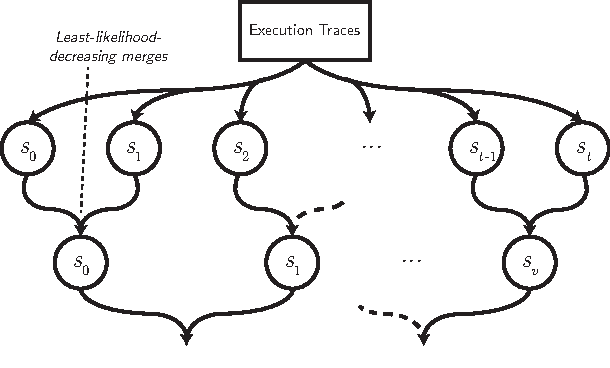
\includegraphics[width=0.8\textwidth]{model-merging-bfmm}
%	\caption{State Merging (Not sure yet whether this should be here)}	% TODO
%	\label{fig:state-merging}
%\end{figure}

%\noindent \textbf{State Merging}:
%\begin{itemize}
%	\item Best-First Model Merging \cite{stolcke1994best}
%	\item State Merging by Trajectory Clustering \cite{nikovski2000learning}
%\end{itemize}
%
%\noindent Other (offline/'data-based') approaches
%
%}

\section{Active Learning}
\label{sec:active-learning}

Devising a completely accurate specification of the \acrshort{acr:mdp}'s transition probabilities typically turns out infeasible for real-world \acrshort{acr:dtp} problems.
However, it should be noted that the learning algorithms that have been addressed earlier, usually recover enough to let an \acrshort{acr:mdp} reflect the actual environment in which an agent operates.
The plans that are derived accordingly from these models yield better performance than a random choice of actions in the execution of the system would.
A class of approaches that we consider in this section are those that combine offline model learning and planning methods with online (reinforcement) learning methods which incrementally update the model parameters.

\subsection{Model-Based Reinforcement Learning}
\label{sec:model-based-reinforcement-learning}

In \acrshort{acr:rl} a distinction exists between model-free and model-based methods, where in the former the choice of action is made based on previously realized value, while the latter evaluates candidate actions based on their expected future rewards.
Model-free or \textit{direct} \acrshort{acr:rl} can therefore be viewed as corresponding to habitual behavior, while model-based \acrshort{acr:rl} corresponds to goal-directed behavior.
When the system under consideration encompasses considerable structure and its dynamics can be modeled accurately, model-based approaches tend to use experiential data more efficiently, be more resilient to changing goals and are better capable of obtaining near-optimal policies \cite{atkeson1997}.
The \acrshort{acr:sdm} problems involving these type of systems are those that qualify for applying model-based \acrshort{acr:rl} in which an initial \acrshort{acr:mdp} could be obtained by offline model learning.
However, one should note that model-free \acrshort{acr:rl} approaches are better suited for learning from scratch (i.e., \acrshort{acr:sdm} problems with very limited prior knowledge and data), as model-based \acrshort{acr:rl} approaches tend to suffer from model bias \cite{deisenroth2011pilco}.
That is, model-based \acrshort{acr:rl} makes the inherent assumption that the underlying model sufficiently accurately reflects the real-world environment.

\newpage

To improve the estimations of the model parameters in model-based \acrshort{acr:rl}, the algorithms demand for efficient exploration, for which various approaches exist that are optimistic in face of uncertainty.
An example is the $E^3$ algorithm \cite{kearns2002near} which explicitly chooses between exploiting the known part of the \acrshort{acr:mdp} and optimally reaching the part that needs to be explored. 
Its exploration is based on \textit{balanced wandering}, which means that the agent will prefer the action that has been executed the least from its current state (breaking ties randomly) until the state has been visited a sufficient number of times.
Another algorithm is the $R$-Max algorithm \cite{Brafman2002}, which has a built-in mechanism for switching between exploitation and exploration and differs in its exploration by letting the agent make the assumption that a maximum possible reward can be obtained from unexplored state-action pairs.

Another issue that should be taken care of in model-based \acrshort{acr:rl} is when and how to update the \acrshort{acr:mdp} and its plan based on acquired experience. A simple approach would be to update the plan on each model update applying a well-known algorithm like \acrshort{acr:vi}, although this is computationally expensive.
To gain efficiency, frameworks like \textsc{RTMBA} \cite{hester2012rtmba} or \textsc{DYNA} and its various extensions \cite{silver2008sample}, aim to update their plans more intelligently (e.g., by updating value functions only for a subset of state-action pairs).
A different approach could be to limit exhaustive exploration of states in the first place, exemplified by the \textsc{RL-DT} algorithm proposed in \cite{hester2010generalized}, which generalizes the effects of actions across states.
This however, is particularly useful for these domains that require sample-efficient learning and for which the available time for exploration is limited.

\subsection{Active Reinforcement Learning}
\label{sec:active-reinforcement-learning}

An appealing approach to overcome inaccuracies of offline learned probabilistic models is to use them as prior models for the model-based \acrshort{acr:rl} algorithms shown in \autoref{sec:model-based-reinforcement-learning}.
In \cite{epshteyn2008active} an approach referred to as \textit{Active \acrlong{acr:rl}} is presented which uses a provided \acrshort{acr:mdp} specification as prior knowledge for exploration through model-based \acrshort{acr:rl}.
Rather than using this \acrshort{acr:mdp} for planning, its model parameters are used as a blueprint for exploration in the actual environment.
The algorithm guides the exploration by selecting these actions for which is known that the `prior' \acrshort{acr:mdp} is most sensitive to changes in the corresponding transition probabilities and rewards.


%\showoutline{
%	\begin{itemize}
%		\item Mention Model-Based \acrshort{acr:rl} or Online Model Learning
%		\item Refer to approach of combining offline and online planning: using an offline-obtained model and policy, apply model-based \acrshort{acr:rl} to update the parameters \cite{epshteyn2008active}
%		\item .....
%	\end{itemize}
%}

\subsection{Bayesian Reinforcement Learning}
\label{sec:bayesian-reinforcement-learning}

\begin{algorithm}[t]
	\caption{Model-Based Bayesian Reinforcement Learning}
	\label{alg:bayesian-reinforcement-learning}
	\begin{algorithmic}[1]
		\Require{Initial \acrshort{acr:mdp} $\mathcal{M} = (\mathcal{S}, s_0, A, \delta, R)$}
		%\Ensure{\acrshort{acr:mdp} $\mathcal{M} = (\mathcal{S}, s_0, A, \delta, R)$} \Comment{$s_0$ and $R$ are here irrelevant}
		\State Initialize prior distribution(s) over unknown parameter(s)
		\Repeat
		\State Select action $a \in A$ based on the posterior distribution(s)
		\State Execute action $a$
		\State Record observed reward and state
		\State Update posterior of unknown parameters based on observations
		\Until Agent terminates
	\end{algorithmic}
\end{algorithm}

Considerable work has been conducted on investigating the application of Bayesian methods to \acrshort{acr:rl} motivated by their close relation to decision theory for making decisions under uncertainty. 
In \textit{\acrfull{acr:brl}} \cite{ghavamzadeh2015bayesian} the idea is to learn a model of the environment by considering the unknown parameters of the model as random variables.
Over these random variables a prior distribution $p(\theta)$ is defined corresponding to the prior beliefs over the unknown parameters $\theta$ of the model.
A common choice for discrete-state and action \acrshortpl{acr:mdp} is a multinomial \textit{Dirichlet} prior, which is parameterized by a count~vector~$\Phi = (\phi_1, \ldots, \phi_k)$ which defines the number of observations of all possible transitions.
Then, as evidence is gathered, the posterior on $\theta$ (which quantifies the uncertainty over the parameters) is updated based on Bayes' rule from which an estimation of the model parameters can be obtained.
A framework that is accordingly used in model-based \acrshort{acr:brl} is the \textit{Bayes-Adaptive \acrshort{acr:mdp}} \cite{guez2012efficient}, which augments the original state space $\mathcal{S}$, transition function $\delta$ and reward function $R$ by jointly combining them with the posterior's hyperparameters $\Phi$.
A general formulation of the steps of model-based \acrshort{acr:brl} is shown in \autoref{alg:bayesian-reinforcement-learning} \cite{png2011bayesian}.

A major drawback of model-based \acrshort{acr:brl} is that obtaining exact solutions appears computationally intractable.
Nonetheless various approximate \acrshort{acr:brl} methods have been devised to provide feasible solutions (such as Bayesian DP, BOSS and Monte-Carlo tree search approaches), of which a majority is summarized in \cite{ghavamzadeh2015bayesian} for the interested reader.
Still, a major challenge is scaling \acrshort{acr:brl} methods to large-scale \acrshortpl{acr:mdp} and models with continuous spaces.
%TODO Maybe rewrite these sentences

%\showoutline{
%\begin{itemize}
%	\item Bayesian Inference (see section 2.2.1)
%	\item BRL: Maintaining a posterior distribution over possible model parameters
%	\item Framework description: \cite{png2011bayesian}
%	\begin{itemize}
%		\item Initialize distributions over unknown parameters (defining a prior, typically Dirichlet distribution)
%		\item Select action based on distributions
%		\item Execute action
%		\item Observe resulting reward and observation
%		\item Update posterior counts of unknown parameters based on observed information
%	\end{itemize}
%	\item MEDUSA, BEETLE + Other examples?
%	\item ..... (To be determined)
%\end{itemize}
%}

% https://people.eecs.berkeley.edu/~avivt/BRLS_journal.pdf

\section{MDP Models with Transition Probability Uncertainty}
\label{sec:mdp-uncertain-probabilities}

Another method to overcome the infeasibility of obtaining completely accurate specifications of transition probabilities is to extend the models and planning algorithms to take imprecise probabilities into account.
Over the years various frameworks have been introduced that utilize this idea, such as the \textit{\acrfull{acr:mdpip}} first introduced in \cite{satia1973markovian} which describes the transition probabilities as a set of linear inequalities to represent incomplete, ambiguous or conflicting beliefs over these probabilities.
That is, in this framework the probability of moving from a state $s_i$ to $s_j$ with action $a$ could for instance be expressed by a variable $p_{ij}$ s.t. a constraint $0 \leq p_{ij} \leq 0.5$.
An illustrative example of a possible application of such a framework would be that of \acrshortpl{acr:mdp} for traffic light control, for which the estimation of lane-turning probabilities for all traffic lanes is problematic, especially as they may be different over the day or throughout the year \cite{delgado2011efficient}.
For these type of domains in particular, the \acrshort{acr:mdpip} framework was devised to account for strict uncertainty in the transition function.
The framework also allows one to find plans under either optimistic or pessimistic assumptions about the true transition function.
However, while the traditional \acrshort{acr:mdpip} framework demands solution techniques that are notably time-expensive, in practice factored \acrshort{acr:mdpip} representations are used for efficient planning, for instance by synchronous dynamic programming based on parameterized algebraic decision diagrams (PADDs) \cite{delgado2011efficient} or \acrshort{acr:rtdp} solutions \cite{delgado2016real}.

An alternative framework is the \textit{\acrfull{acr:bmdp}} where a range of the transition probabilities and rewards are known, such that it can be viewed as a set of possible \acrshortpl{acr:mdp}.
In fact, \acrshortpl{acr:bmdp} are a special case of \acrshortpl{acr:mdpip} where the attainable probabilities can be defined by a discrete set rather than linear constraints, but where ranges can also be defined on the rewards.
When it is possible to restrict the parameters of the \acrshort{acr:mdp} at intervals as is done in the \acrshort{acr:bmdp} framework, the algorithms that exist for \acrshortpl{acr:bmdp} exploit the restricted structure of the parameters more efficiently than \acrshortpl{acr:mdpip}, because the \acrshort{acr:mdpip} solutions demand \acrshort{acr:lp} approaches in each iteration.
There exist solution techniques for \acrshortpl{acr:bmdp} that can efficiently learn optimal policies, such as \textit{interval \acrshort{acr:vi}} \cite{givan2000bounded} or robust versions of \acrshort{acr:rtdp} \cite{buffet2005robust}.


%\section{Gaussian Process Dynamics}
%\label{sec:gp-dynamics}
%http://machinelearning.wustl.edu/mlpapers/paper_files/ICML2011Deisenroth_323.pdf

% TODO;s
%% Fitting Markov Chains/MDPs:
	% Refer back to section 2.2.1:
	% - likelihood maximization
	% - Bayesian inference/optimization
%% Fitting HMMs/POMDPs:
	% ITERATIVE ADJUSTMENT OF PROBABILITIES:
	% - Baum-Welch Algorithm
	% - Gradient-Ascent in Likelihood
	% STATE MERGING
	% - Best-first
	% - Trajectory clustering
%% Reinforcement Learning: Online Model Learning

%% However, most of the previous works assume the state-space of the probabilistic model to be known.

%\section{Bayesian Reinforcement Learning}
%\label{sec:bayesian-reinforcement-learning}

% 

%
%\section{Overview}
%\label{sec:related-work-overview}
%
%% 
\chapter{Model-Learning Framework}
\label{ch:methodology}
%TODO State clearly again our problem, what we are going to do and why we want to do it (but in little more detail where necessary than in the introduction). See the *-TODO
%TODO Explain how we would like to see the exploration/data acquisition to be performed. Dataset should appropriately ('of sufficient quality') reflect the dynamics of the system so that an accurate representation in the form of an MDP can be learned from it.
%TODO Use the mobile robot navigation domain as a **running example** application rather than putting it in the last section of the chapter
%TODO Explain the components that we learn/derive (state space and transition function and accordingly reward functions) and which components are fixed (actions)
%TODO Devote a paragraph clearly on how the reward function is defined; multiply the reward with the discrepancy factor rather than the value 

Our interest in this thesis lies in the development of probabilistic models for systems whose dynamics are stochastic.
The objective is to use a dataset of execution traces of a system to attain an accurate system representation, which can be used to obtain plans for optimal automated control of the system under consideration.
In this chapter we describe our proposed framework that applies learning algorithms to obtain probabilistic models in the form of \acrshortpl{acr:mdp} and optimizes for a performance-maximizing model by sampling multiple hyper-parameter settings for these learning algorithms.

In \autoref{sec:model-learning-routine} a detailed explanation is provided of the learning and optimization routine which forms the basis of our framework.
Then in \autoref{sec:cost-effective-optimization} the framework is extended such that it consists of three cost-incremental phases.
Finally, in \autoref{sec:application-mobile-robot} a possible application (i.e., mobile robot navigation) of the framework is discussed, which is also used for evaluating the approach through the experiments that have been carried out and which are described in \autoref{ch:experimental-results}.

\section{Model Learning and Optimization Routine}
\label{sec:model-learning-routine}

%TODO * See comment at the top; Expand on these paragraphs
As the development of probabilistic models oft to be a difficult an time-costly process for a human designer, an appealing idea is to automate the model development process by applying learning algorithms on a dataset of execution traces of the system under consideration.
However, to achieve effective planning in a real-world environment, the models that are learned should accurately reflect the dynamics of the system.

There are two major reasons for a learned model to not yield good performance.
First of all, the learned model may be too complicated for the amount of available data, which leads to model over-fitting.
On the other hand, one could acquire a model that is too simple to explain the available data and so does not accurately reflect the underlying system in that situation.
Therefore, the parameters of the learning algorithm should be properly adjusted in order to obtain accurate probabilistic models.

The learning and optimization routine described in this section, depicted in \autoref{fig:learning-routine-complete}, aims to achieve this by posing the adjustment of these parameters as an optimization task, with the objective of obtaining an \acrshort{acr:mdp} model that maximizes the performance of executing the plans that are derived from it.

\begin{figure}[t]
	\centering
	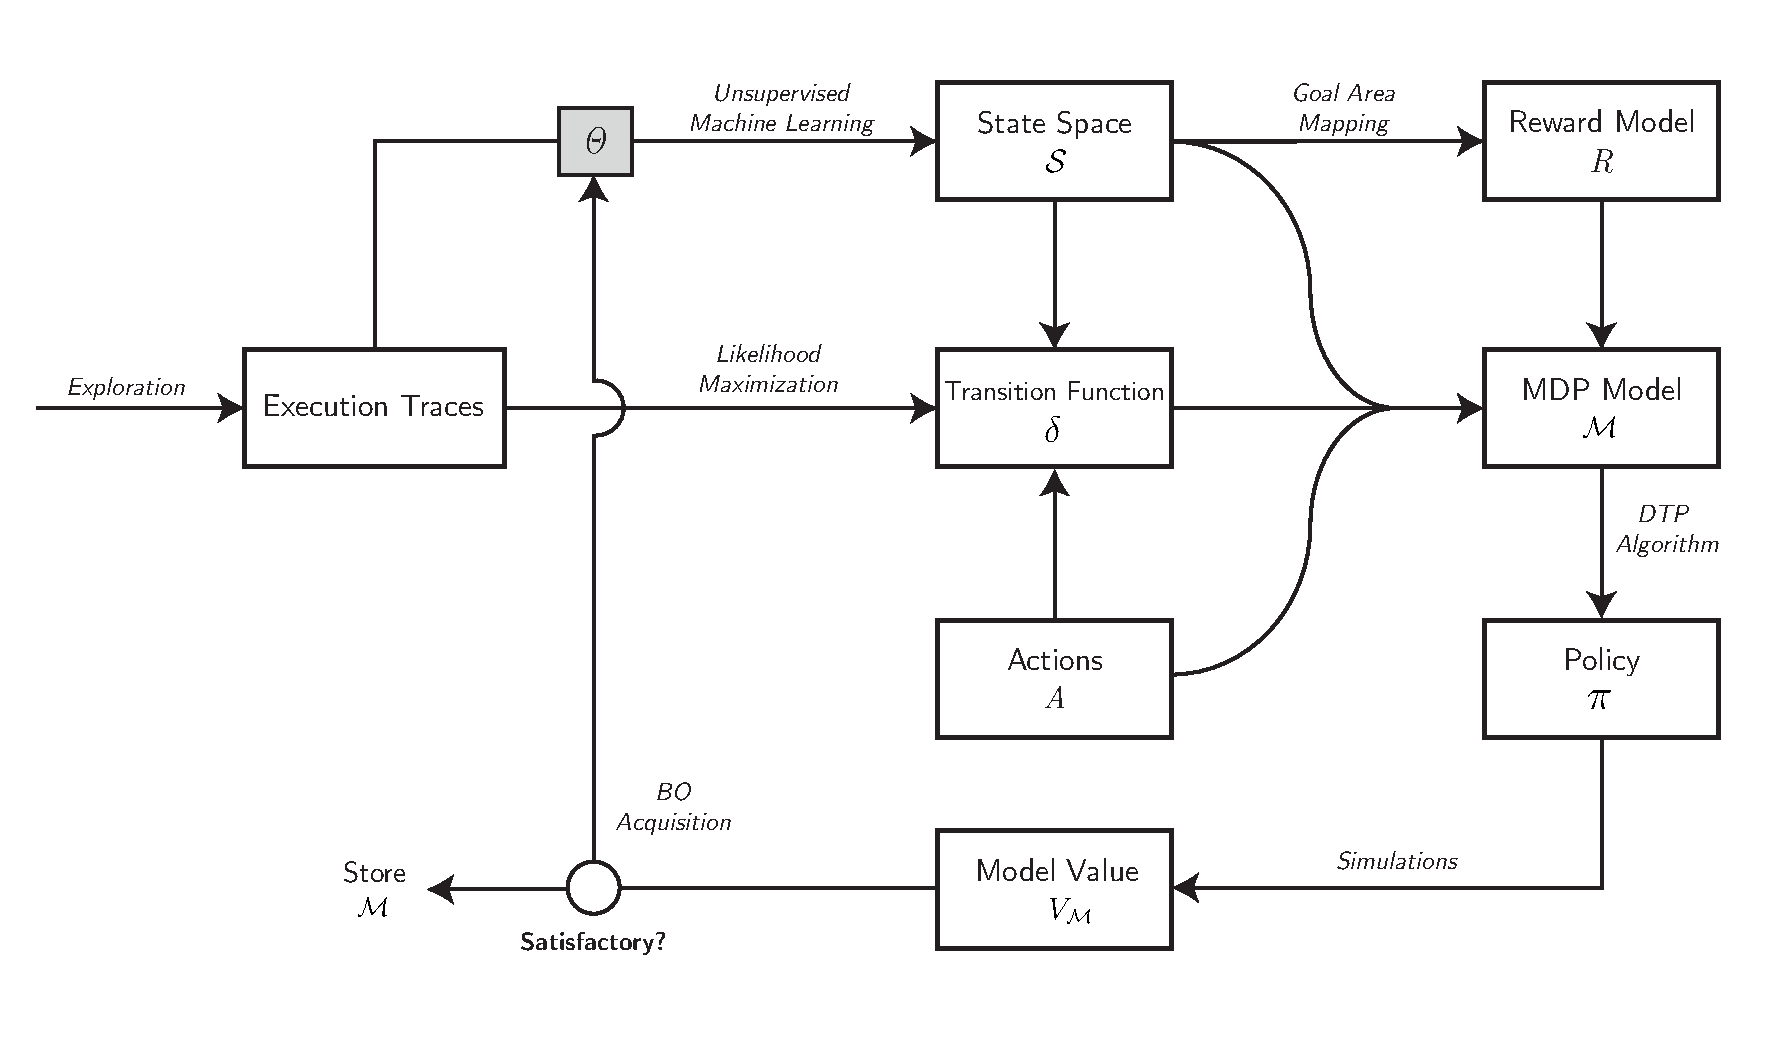
\includegraphics[width=\textwidth]{learning-cycle-complete-v22}
	\caption{Diagram of the model learning and optimization routine.}
	\label{fig:learning-routine-complete}
\end{figure}

\subsection{Learning Step}
\label{sec:learning-step}

The routine can be viewed as consisting of two subsequent steps which are repeated until an \acrshort{acr:mdp} model that yields satisfactory performance is obtained.
The first of these two main steps will be referred to as the \textit{learning step}, in which an \acrshort{acr:mdp} model is acquired.
This learning step starts off with a data-set of execution traces obtained beforehand.
Given a parameter-setting $\theta$ for a selected unsupervised machine learning algorithm, a state-space $\mathcal{S}$ is acquired using the execution traces as training set.
Subsequently a transition function $\delta$ is acquired by applying a known model-learning (as described in \autoref{sec:learning-probabilistic-models}) given the data-set, state-space $\mathcal{S}$ and possible actions $A$.
The goals of the system are accordingly mapped to a reward function $R$ over the acquired state-space $\mathcal{S}$ (or alternatively over state-action pairs or state-action-state triplets).
The state-space $\mathcal{S}$, transition function $\delta$, action set $A$, reward function $R$ and a configurable initial state $s_0$ are then combined into an \acrshort{acr:mdp} $\mathcal{M} = (\mathcal{S}, s_0, A, \delta, R)$.

To assess the performance yielded by $\mathcal{M}$, the \acrshort{acr:mdp} is solved by applying known \acrshort{acr:dtp} algorithms like \acrshort{acr:vi} or \acrshort{acr:pi} to obtain policies for a set of tasks the system is expected to perform.
The value of the model $V_{\mathcal{M}}$ is then determined by checking how well the system is expected to perform by execution according to the derived policies (e.g., based on simulations and/or the value function obtained by a \acrshort{acr:dtp} algorithm).
\autoref{sec:performance-measure} describes in detail how the performance yielded by the learned \acrshortpl{acr:mdp} is assessed and how a fair comparison of different \acrshortpl{acr:mdp} may be achieved for this routine.

%\begin{itemize}
%	\item Start off with data-set of execution traces obtained beforehand
%	\item A number of parameter-settings $\theta$ for the model-learning are initially sampled at random from a designer-specified domain $\Theta$ (i.e., the parameter-space).
%	\item Acquire state-space by an unsupervised machine learning method
%	\item Acquire transition function by applying a known model-learning algorithm as in \autoref{sec:learning-probabilistic-models} (e.g., a maximum likelihood approach)
%	\item Goals are mapped to a reward function $R$ over the acquired state-space $\mathcal{S}$ (or possibly over state-action pairs or state-action-state triplets)
%	\item Then the state-space $\mathcal{S}$, transition function $\delta$, action set $A$, reward function $R$ and a configurable initial state $s_0$ form an \acrshort{acr:mdp} $\mathcal{M} = (\mathcal{S}, s_0, A, \delta, R)$.
%	\item To asses the associated performance or value of $\mathcal{M}$, we solve the \acrshort{acr:mdp} using known \acrshort{acr:dtp} algorithms like \acrshort{acr:vi} (see \autoref{sec:planning}) to obtain one or more policies $\pi$.
%	\item The value of the model $V_\mathcal{M}$ is then determined by checking how the system would perform by execution according to the derived policies (e.g., based on simulations and/or the value function of \acrshort{acr:vi}).
%\end{itemize}

\subsection{Optimization Step}
\label{sec:optimization-step}

The second main step of the routine will be referred to as the \textit{optimization step}, in which a parameter-setting $\theta$ is selected for the next learning step in such way that yielded performance converges to a global maximum as quickly as possible.
As initially there is no knowledge of the performance given the settings of the learning parameter(s) $\theta$, in the first few routine-iterations parameter-settings are selected at random from the designer-specified domain $\Theta$ (i.e., the parameter-space).
Together with the value $V_{\mathcal{M}}$ of the corresponding model obtained in the learning step for each of these parameters $\theta$, they are stored in an evidence set $\mathcal{D}$.
The objective function $f: \Theta \mapsto \mathbb{R}$ is then defined such that it maps parameter-settings $\theta \in \Theta$ to real-valued performance yielded by \acrshortpl{acr:mdp}.

As discussed earlier in  \autoref{sec:bayesian-optimization-problem}, the objective functions for the class of \acrshort{acr:sdm} problems tend to be expensive to evaluate as proper estimations can only be made through expensive simulations.
Therefore, \acrlong{acr:bo} emerges as an attractive method to find a global maximizer $\theta^\ast \in \Theta$ for our objective function.
After each iteration the evidence set $\mathcal{D}$ is augmented with a new observation, based on which the posterior $p(f\vert \mathcal{D})$ of the objective function $f$ is updated accordingly.
A new parameter-setting for the next learning step is then sampled, corresponding to maximal utility in the selected acquisition function.

%\begin{itemize}
%	\item As said, at first a number $n$ of parameter-settings are selected randomly, stored in evidence set $\mathcal{D}$.
%	\item For these parameter-settings we obtain an estimation of the performance of executing plans derived from the learned \acrshortpl{acr:mdp}
%	\item Define the objective function $f$ such that it maps parameter-settings $\theta$ to real-valued model performance $f: \Theta \mapsto \mathbb{R}$ 
%	\item Bayesian Optimization: Motivate the application of this method to these type of problems `again'. Defines prior over $f$ and posterior based on the gathered evidence in $\mathcal{D}$.
%	\item New evidence is then acquired based on the utility function used in the optimization.
%\end{itemize}

\subsection{Performance Measure}
\label{sec:performance-measure}

\begin{figure}[t!]
\centering
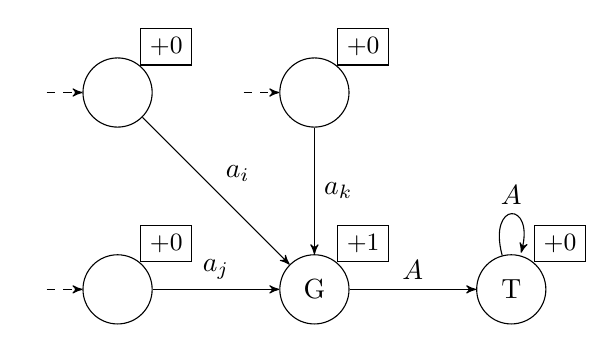
\begin{tikzpicture}[->,>=stealth',auto,node distance=2.5cm,every label/.style=draw,every initial by arrow/.style={dashed}]
\tikzstyle{every state}=[fill=white,draw=black,text=black,scale=1]	% thick
\node[state,initial,initial text={},label={50:\small$+0$}] (s1) {};
\node[state,initial,initial text={},label={50:\small$+0$}] (s2) [below of=s1] {};
\node[state,initial,initial text={},label={50:\small$+0$}] (s3) [right of=s1] {};
\node[state,label={50:\small$+1$}] (goal) [below of=s3] {G};
\node[state,label={50:\small$+0$}] (trap) [right of=goal] {\text{T}};
\coordinate (con) at (0,2);
\path
(s1)
edge node {$a_i$} (goal)
(s2)
edge node {$a_j$} (goal)
(s3)
edge node {$a_k$} (goal)
(goal)
edge node {$A$} (trap)
(trap)
edge [loop above] node {$A$} (trap)
;
%\draw [->, dashed, shorten >=0pt] (s3) to[right] node[auto] {} ++(1.3,0)
;
\end{tikzpicture}
\caption{One-time reward in goal state G in an \acrshort{acr:mdp} realized by a trap state T.}
\label{fig:goal-trap-state}
\end{figure}

Posing the learning of probabilistic models as an optimization task requires us to define a mapping of \acrshortpl{acr:mdp} to a performance measure that can fairly compare different models.
As discussed earlier, one can express the performance of an \acrshort{acr:mdp} in terms of how well the agent performs tasks following policies that are derived from the model.
Therefore, one option is to make use of the value function $V$ obtained by a \acrshort{acr:dtp} algorithm (e.g., \acrshort{acr:vi} or \acrshort{acr:pi}).

One problem that emerges, however, is that there might not be a one-to-one correspondence between learned and true (goal) states, which leads to the possibility of small state spaces yielding high value while the goal states might not map well to the true goal states.
To take care of this, we introduce a discrepancy factor $\xi \in [0, 1]$, which corresponds to the fraction of data points within the goal state that map to the true goal.

Accordingly, a possible expression of how well the agent executes its task then is:
\begin{equation}
\label{eq:vdtp}
V_{\mathit{DTP},(s_0,R)} = \xi \cdot V[s_0]
\end{equation}
where $s_0 \in \mathcal{S}$ is the initial state and $R$ the reward function of the \acrshort{acr:mdp} for the task.

However, although the \acrshort{acr:dtp} algorithm may yield high value for the task, it might be that the agent will not perform well following the policy in the real world.
To better assess the performance, one could execute simulations in which the agent follows the policy derived from the \acrshort{acr:mdp} model.
Although performing simulations is more cost-expensive, it yields a better approximation of how well the agent executes a task following a policy obtained from the model.
Accordingly, let us express the performance on a task in the simulations as:
\begin{equation}
\label{eq:vsim}
V_{\mathit{SIM}, (s_0, R)} = \gamma^{t} \cdot R[i]
\end{equation}
where $s_0 \in \mathcal{S}$ is the initial state, $R$ the reward function, $\gamma$ the discount factor, $i \in \mathcal{S}$ the goal state and $t$ the number of steps taken to reach the goal.

Combining the expressions of \autoref{eq:vdtp} and \autoref{eq:vsim} yields the following expression of the performance on a task:
\begin{equation}
\label{eq:vcom}
\beta \cdot V_{\mathit{DTP}, t=(s_0, R)} + (1 - \beta) \cdot V_{\mathit{SIM}, t=(s_0, R)}
\end{equation}
where $\beta \in [0, 1]$ is a parameter which specifies the relative weight of $V_{\mathit{DTP}, t}$ against that of $V_{\mathit{SIM}, t}$ and where $s_0$ and $R$ are the initial state and reward function for the task respectively.

As the desire is to obtain a well-generalizing model that performs well on different tasks, we estimate the performance by obtaining the value yielded for multiple tasks.
To achieve this, let us first define multiple starting configurations and multiple goals for the system.
The starting configurations are each mapped to corresponding states in the \acrshort{acr:mdp}, so that one can define $\mathcal{S}_0 \subseteq \mathcal{S}$ as a set of initial states.
Similarly, the goals are each mapped to states, such that one can define $\mathcal{S}_G \subseteq \mathcal{S}$ as a set of goals.
Let us then define $R_G$ as a set of reward functions $R_i$ for each $i \in \mathcal{S}_G$ in which a one-time reward (which is realized as depicted in \autoref{fig:goal-trap-state}) is received only in goal-state $i$.
The reason the reward can only be obtained once is because in that case $V_{\mathit{DTP}, t}$ and $V_{\mathit{SIM}, t}$ will be in the same range.
Then accordingly we can define $T = \mathcal{S_0} \times R_G$ as the set of tasks, in the form of all pairs of initial and goal states, over which the performance is assessed.

\noindent Putting this all together, the performance of an \acrshort{acr:mdp} $\mathcal{M}$ can in this way be expressed as:
\begin{equation}
\label{eq:vm}
	V_{\mathcal{M}} = \frac{\sum_{t \in T} \beta \cdot V_{\mathit{DTP}, t} + (1 - \beta) \cdot V_{\mathit{SIM}, t}}{|T|}
\end{equation}
where $T$ is the set consisting of the pairs of initial states and reward functions of the tasks over which the performance is assessed.

% There have been debates about the performance
% measure that should be maximized during learning {
% one point of view is that the available data should be
% used to learn all possible perceptual distinctions in the
% real world while the opposite view
% would have it that only those distinctions that are utile in actual planning and control should
% be learned [McC92]. Those algorithms that learn only utile distinctions use either decision trees
% or instance-based learning to form state representations.

%The value of \acrshort{acr:mdp} $\mathcal{M}$ is defined as:
%\begin{equation}
%	V_{\mathcal{M}} = \beta \cdot V_\mathit{DTP} + (1 - \beta) \cdot V_\mathit{SIM}
%\end{equation}
%where $\beta \in [0, 1]$ is a parameter which specifies the relative weight of $V_\mathit{DTP}$ against that of $V_\mathit{SIM}$.
%
%\begin{itemize}
%	\item Multiple starting positions/initial states
%	\item Multiple goals/reward functions
%	\item $V_\mathit{DTP}$, how to deal with problem of less states -> less steps. Need fair comparison.
%	\item Discrepancy factor; obtained value based on part of the state covering the goal
%	\item Goal state to trap state to avoid acquiring unlimited reward
%\end{itemize}

% One of the main issues faced in learning \acrshort{acr:mdp} models is that of deciding on the state space, while one typically does not know the size of the true state space of the real-world process that generated the training data.
%In fact this state space might even have been continuous, while the state space of the model is typically discrete.
%In particular this might form an issue in the planning phase where a reward function needs to be defined to express the goals in the \acrshort{acr:mdp}, for which there may not be a clear one-to-one mapping from real-world states to model states.

% Two approaches:
% - Clustering training data to obtain states
% - Trajectory Clustering

\section{Cost-Incremental Optimization}
\label{sec:cost-effective-optimization}

\begin{figure}[t]
	\centering
	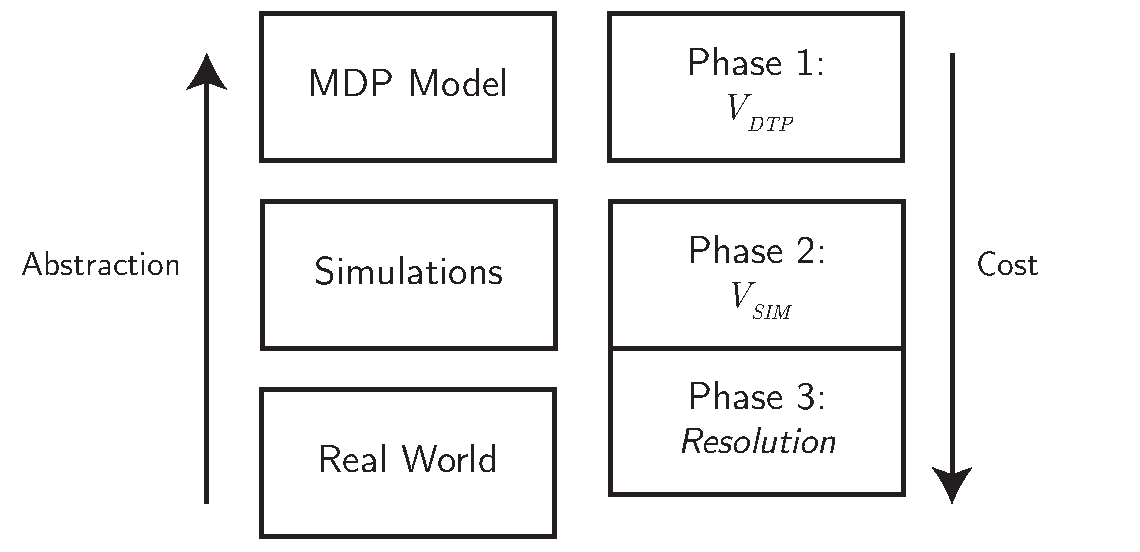
\includegraphics[width=0.7\textwidth]{abstraction-5-1}
	\caption{Correspondence of the phases of the model learning framework to the different levels of abstraction.}
	\label{fig:abstraction-cost}
\end{figure}

To make the solution more cost-effective, the framework is extended by defining three phases with the aim of exploiting the lower cost of computing the value function for \acrshortpl{acr:mdp} in comparison to the cost of executing plans in simulations or the real world.
That is, assessing performance solely based on learned \acrshort{acr:mdp} models is less cost-expensive, although the model might not accurately reflect the real world as its abstracts over low-level details.
This section defines the phases of the extension, of which each subsequent phase better reflects the real world, but on the other hand are accompanied by higher costs as is depicted in \autoref{fig:abstraction-cost}.

%\blindtext

%\begin{itemize}
%	\item Change the $\beta$-parameter of Eq 5.1 over time
%	\item The $\gamma$ discount factor (low values $\to$ faster planning)
%	\item Three 'phases':
%\end{itemize}

\afterpage{
	\begin{figure}[t]
		\centering
		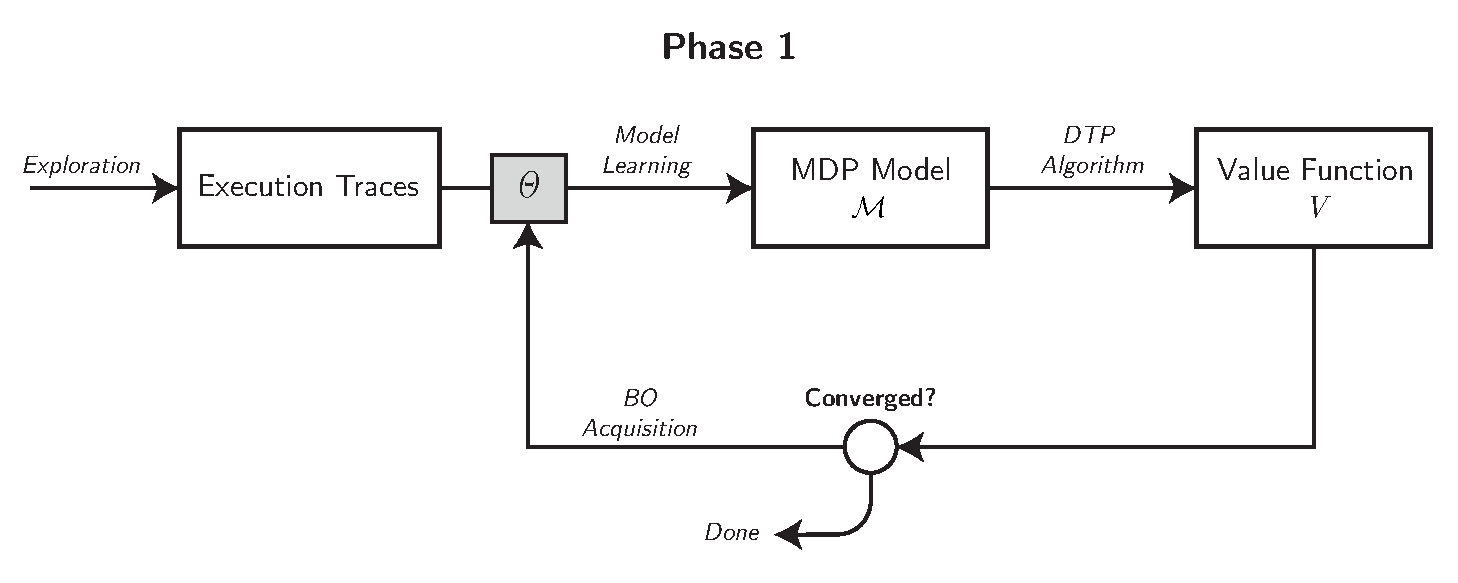
\includegraphics[width=1.0\textwidth]{phase-1.pdf}
		\caption{Block diagram showing the steps of the first phase of the cost-incremental optimization framework. This phase develops a distribution which reflects the interesting area of the parameter space solely based on the value functions of \acrshortpl{acr:mdp}.}
		\label{fig:phase-1}
	\end{figure}
	
	\begin{figure}[t]
		\centering
		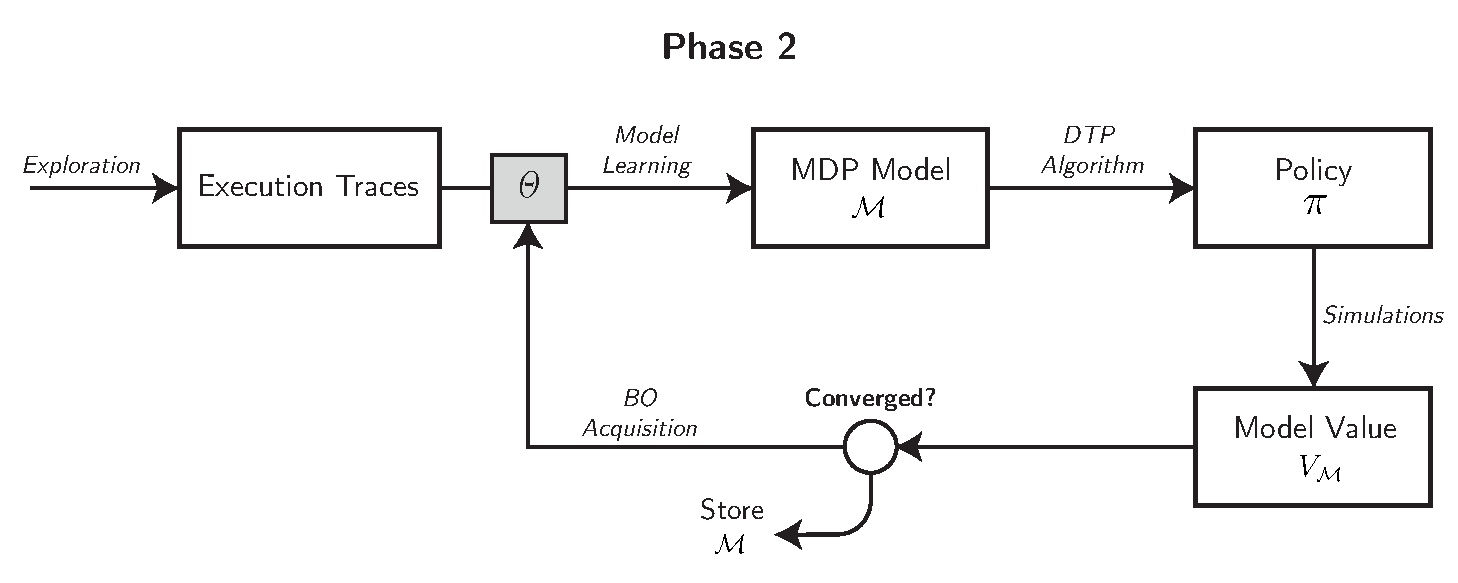
\includegraphics[width=1.0\textwidth]{phase-2.pdf}
		\caption{Block diagram showing the steps of the second phase of the cost-incremental optimization framework. This phase uses the distribution learned in the first phase as a prior and optimizes for an \acrshort{acr:mdp} which maximizes performance in simulations.}
		\label{fig:phase-2}
	\end{figure}
	
	\begin{figure}[t!]
		\centering
		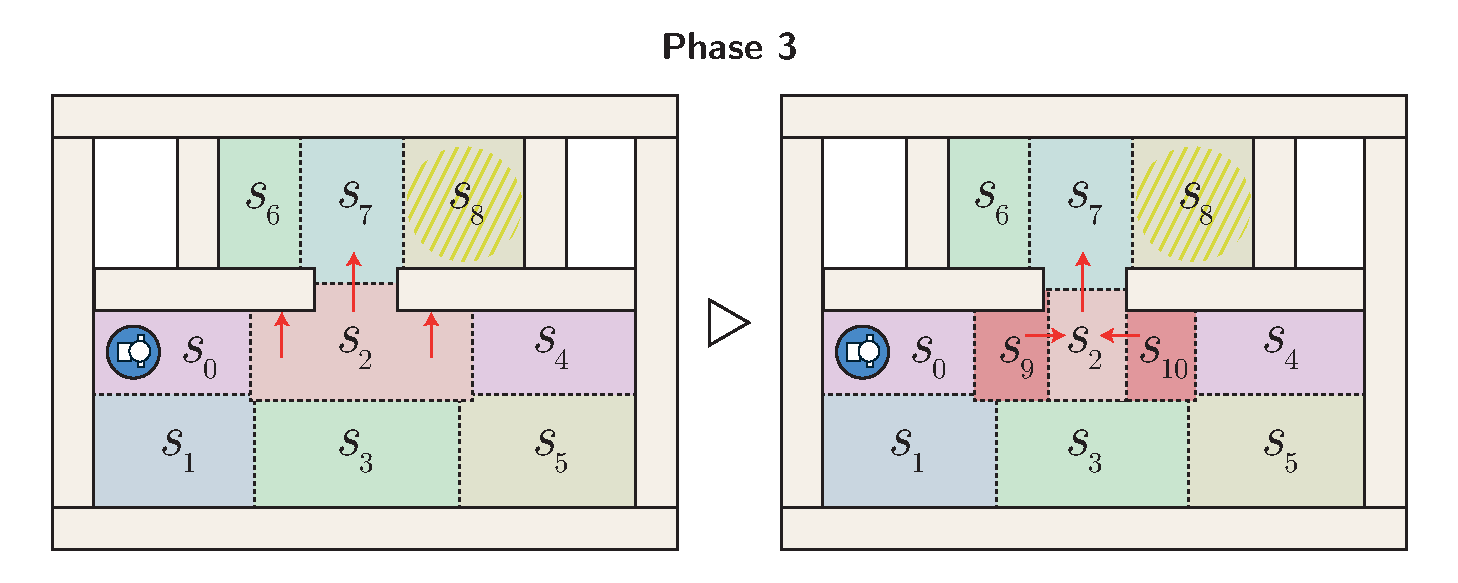
\includegraphics[width=1.0\textwidth]{phase-3.pdf}
		\caption{An illustration of the goal of the third phase in the context of mobile robot navigation. In the navigation towards the goal state $s_8$, the robot might get stuck in state $s_2$ following the optimal policy. Therefore higher resolution is needed in this area of the state space.}
		\label{fig:phase-3}
	\end{figure}
	\clearpage
}

\subsection{Phase 1: Value Function Pre-Processing}
\label{sec:phase-1}

In the first phase the performance is assessed solely based on the value functions derived by the \acrshort{acr:dtp} algorithm used for planning.
This means the $\beta$ parameter is set to $\beta = 1$ such that the performance $V_{\mathcal{M}}$ of \acrshort{acr:mdp} $\mathcal{M}$ is expressed only in terms of $V_\mathit{DTP}$ and so no simulations are performed in this phase.
Therefore, this first phase is relatively cost-cheap, and although it abstracts from the real-world the most, it may be used to identify the interesting area of the parameter space.
Hence, the goal of this first phase is to narrow down the search space to a subspace of learning parameters more likely to yield high performance.

The block diagram in \autoref{fig:phase-1} depicts the main steps of this first phase. The execution traces from the exploration are used to obtain \acrshortpl{acr:mdp} by applying the learning algorithms given a parameter-setting $\theta$.
The value of a learned model $\mathcal{M}$ is then only based on the value functions $V$ for a set of tasks $T$ the system is expected to perform.
The value of model $\mathcal{M}$ is thus computed as:
\begin{equation} 
V_{\mathcal{M}} = \frac{\sum_{t \in T} V_{\mathit{DTP}, t}}{|T|}
\end{equation}
where each task $t \in T$ is defined in terms of an initial state and reward function.
Based on the gathered evidence new parameter-settings $\theta$ are sampled iteratively, which are those settings for which the utility is the highest in the acquisition function used for \acrshort{acr:bo}.
This continues until a stopping condition has been met, where in this first phase stopping after a fixed number of iterations should be acceptable, as the goal is only to narrow down the search space.
At the end of the first phase, the resulting posterior \acrshort{acr:gp} distribution is taken and used as a prior for the next optimization phase.

%In practice this could be done by setting a threshold, say, $\eta \in [0, 1]$, that specifies the allowed deviation from the observed maximum in the evidence set $\mathcal{D}$, i.e. $\max_\mathcal{(x_i, y_i) \in D} y_i$, which can be used to define parameter bounds based on the posterior mean.

%\fbox{\textbf{TODO:} Update threshold to prior.}

%First phase: Performance assessment solely based on $V_\mathit{DTP}$ (i.e., initially $\beta = 1$). No simulations. $\gamma$ parameter starts off low and increases over time. This means this first phase is relatively cost-cheap, but might give us a global idea of the interesting area of the parameter-space so that we could narrow this space down.

%\blindtext

\subsection{Phase 2: Simulation-Based Optimization}
\label{sec:phase-2}

The second phase exploits the knowledge gathered in the first phase by using it as a \acrshort{acr:gp} prior in a new optimization process such that it starts off in the part of the parameter space most likely to yield high value.
In this phase the performance assessment becomes more cost-expensive, but is also made more accurate by performing simulations and weighing the observed $V_\mathit{SIM}$ in the performance measure.
This means, we either fix the $\beta$ parameter to a value in $[0, 1)$, or alternatively, gradually decrease it over time so that $V_\mathit{SIM}$ plays a more significant role the more iterations have passed.

The block diagram of \autoref{fig:phase-2} depicts the main steps of this second phase.
The same execution traces from the exploration are again passed to model learning algorithms to obtain \acrshortpl{acr:mdp} given parameter-settings $\theta$.
What is first of all different is that the acquisition of new samples is steered by the prior obtained from the first phase.
Secondly, the value is now determined by simulations in which the policies emerging from a learned model $\mathcal{M}$ are followed for the tasks that the agent is expected to perform.
This value $V_\mathcal{M}$ is thus computed as in \autoref{eq:vm} with a weight factor $\beta > 0$.
The optimization process continues until a stop condition, which could be either reaching a fixed number of iterations, a fixed time or a stopping criterion (e.g., when potential improvement becomes negligible).
At this point we can obtain an \acrshort{acr:mdp} most likely to yield high performance for the problem under consideration.

%Second phase: $\beta$ decreases over time, which means $V_\mathit{SIM}$ starts to play a role, and assessment becomes more accurate, but also more cost-expensive.

%\blindtext

\subsection{Phase 3: Resolution Post-Processing}
\label{sec:phase-3}

The last phase starts when the parameter space has been narrowed down sufficiently or the parameter search has converged to an optimum.
In this phase, the goal is to further improve learned models by checking whether the transition probabilities are likely to match reality.
The identification of discrepancies in these probabilities happens by executing actions in those areas of the state-space that are visited most often and in which the agent tends to get stuck (according to the transition probabilities) and seeing if the observed transitions yield comparable probabilities.
For those areas and their corresponding states for which mismatches are identified, higher resolution is provided to better reflect the system's dynamics in the real world.

The illustration of \autoref{fig:phase-3} aims to clarify the goal of this third phase by means of an example for the context of mobile robot navigation.
Although the model obtained in the previous phase, might yield high performance for most of the tasks used to assess model value, a situation as illustrated in this figure might occur.
That is, in the figure the robot, depicted in blue, needs to move from its current position to the goal, indicated by the yellow shaded area.
For the state space depicted on the left-side however, the robot might get stuck following the optimal policy from which the need for higher resolution in this area emerges.
% To identify these discrepancies we could check if the transition probabilities of the model match observed outcomes of actions from the different states of the model.

%Third phase: Starts when the parameter-space has sufficiently been narrowed down. To further improve learned models we would like to see if the opportunity exists of having higher resolution in some areas of the state space to better reflect the data-set.

%\blindtext

\section{Application to Mobile Robot Navigation}
\label{sec:application-mobile-robot}

\begin{figure}[t]
\centering

\captionsetup{font=small}
\captionsetup[subfigure]{font=footnotesize}
\captionsetup[subfigure]{justification=centering}
\begin{subfigure}{.5\textwidth}
	\centering
	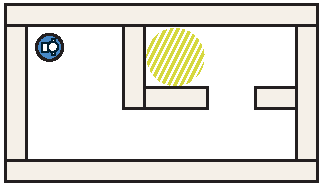
\includegraphics[width=.8\linewidth]{dummy-map-2-1}
	\caption{Dummy environment with a mobile robot and goal area.}
	\label{fig:dummy-map-1}
\end{subfigure}\hfill
\begin{subfigure}{.5\textwidth}
	\centering
	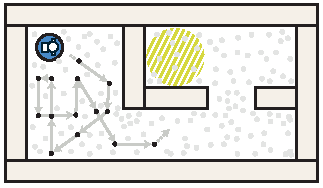
\includegraphics[width=.8\linewidth]{dummy-map-2-2v2}
	\caption{Data-points of execution traces from exploration depicted.}
	\label{fig:dummy-map-2}
\end{subfigure}

\bigskip

\begin{subfigure}{.5\textwidth}
	\centering
	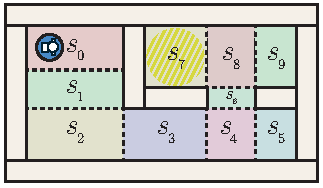
\includegraphics[width=.8\linewidth]{dummy-map-2-3}
	\caption{State-space of a learned \acrshort{acr:mdp} depicted.}
	\label{fig:dummy-map-3}
\end{subfigure}\hfill
\begin{subfigure}{.5\textwidth}
	\centering
	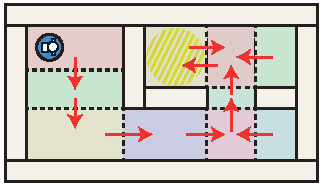
\includegraphics[width=.8\linewidth]{dummy-map-2-4}
	\caption{Corresponding optimal policy for the \acrshort{acr:mdp}.}
	\label{fig:dummy-map-4}
\end{subfigure}
	\caption{Planning for the navigation of a mobile robot by learning \acrshortpl{acr:mdp} from data about the environment.}
\end{figure}

%\begin{itemize}
%	\item Description
%	\item Motivation of this application
%	\item Generalization to other applications
%	\item Details on how we apply the framework to this application
%\end{itemize}

An example application for which the model learning framework described in this chapter could be used is that of mobile robot navigation.
The problem statement is that an agent has control over a mobile robot that should be able to navigate from one location to another in an open world, say, an office environment, as fast as possible.
This problem domain is particularly suited as the robots oft to operate under significant uncertainty in their actions (e.g., slipping) and observations (e.g., sensor noise).
Although there are other potential applications as we described in \autoref{ch:introduction}, this particular application can be used to illustrate the complete procedure of learning \acrshort{acr:mdp} from data and obtaining plans accordingly quite well.

For example, let us consider the scenario in which the robot needs to operate in an environment as depicted in \autoref{fig:dummy-map-1}.
Then, before our model learning framework is applied to learn \acrshortpl{acr:mdp} for the system, the data about the environment could have been obtained in the form of execution traces that consist of logs of the robot's location and the (next) action it's about to take.
This could then give a set of data-points, as depicted in \autoref{fig:dummy-map-2}, which can be used to learn the states and transition probabilities of an \acrshort{acr:mdp}.
A potential state-space of an \acrshort{acr:mdp} that might be learned from this dataset is shown in \autoref{fig:dummy-map-3}.
Then, assigning a reward to a state that covers the goal area should give us a policy that leads the robot from any initial state to the goal state as depicted in \autoref{fig:dummy-map-4}.

In this application the performance of a learned \acrshort{acr:mdp} can be assessed as described in \autoref{sec:performance-measure} through the computed value function and performing simulations for the various tasks the robot should be able to execute.
Comparing the performance that was assessed for multiple \acrshortpl{acr:mdp} through the framework on convergence leads to an \acrshort{acr:mdp} that reflects the real world and generalizes over multiple tasks quite well.




%% OLD %%

%\textbf{Note:} These bullet-points have not been completely updated yet although most are still relevant. Outline should be such that we first discuss the framework for model learning and optimization without considering incomplete data or doing cost-sensitive optimization, which are discussed next ('why and how').
%Probably describing the framework should be separated from the application to mobile robot navigation and how it is implemented, which should be described afterwards.
%
%\begin{itemize}
%	\item Introduction
%	\item Explain high-level algorithm idea?
%\end{itemize}
%
%\section{Application}
%\label{sec:application}
%
%% 
%
%\begin{itemize}
%	\item Mobile robot navigation
%	\item Why this application?
%	\item Generalization possible to other applications?
%\end{itemize}
%
%\section{Exploration Phase}
%\label{sec:exploration-phase}
%
%% 
%
%\begin{itemize}
%	\item Obtain a dataset of observations, for our application this concerns data about attainable positions of the robot that will be controlled
%	\item Under the assumption such a dataset is not yet available to us, this dataset is retrieved in an exploration phase
%	\item In this exploration phase, the robot should explore the environment and periodically record information about its current position while aiming to visit all the locations of importance
%	\item This exploration phase is (preferably) only carried out once
%	\item To obtain a dataset for our tests the exploration phase is carried out in a robot simulator. Should also explain what data is obtained in this exploration.
%	\item The overall algorithm is tested for multiple maps/(office-like) environments, which might differ in their dimensions, number of obstacles or `openness'.
%	\item To take into account dynamically changing environments to some extent, there are also doors that will be open or closed as time passes.
%	\item The simulations are carried out in the Morse simulator, in which the exploration is carried out by an agent that randomly navigates an environment.
%\end{itemize}
%
%\section{State Space Acquisition}
%\label{sec:state-space-aggregation}
%
%% 
%
%\begin{itemize}
%	\item Using exploration data
%	\item Unsupervised machine learning to obtain states for an MDP model (various possible methods possible: e.g., kmeans, gmm)
%	\item Unknown parameter $\delta$ of the unsupervised machine learning algorithm to be optimized
%\end{itemize}
%
%\section{Model and Policy Acquisition}
%\label{sec:model-policy-acquisition}
%
%% 
%
%\begin{itemize}
%	\item State space obtained as described in previous section
%	\item Transition function obtained based on exploration data and state space through the likelihood maximization approach.
%	\item For our application the actions are fixed and can either be \textsc{NORTH}, \textsc{EAST}, \textsc{SOUTH}, \textsc{WEST} which makes the robot navigate in the corresponding direction.
%	\item Rewards
%	\item Timesteps
%	\item Policy (various possible `solvers': value iteration, policy iteration)
%\end{itemize}
%
%\section{Bayesian Model Optimization}
%\label{sec:bayesian-model-optimization}
%
%% 
%
%\begin{itemize}
%	\item Optimization of the unknown $\delta$ parameter of the machine learning algorithm for state space aggregation
%	\item Evaluation by simulations of the found policy for the given $\delta$ parameter
%	\item ...
%\end{itemize}
%

\chapter{Experimental Setup and Results}
\label{ch:experimental-results}

%vTODO Add a section illustrating the implementation; giving some examples of how clustering algorithms are used to define a state-space and learn an MDP based on likelihood maximization and how this MDP is used to navigate the robot in an environment.

%\begin{itemize}
%	\item Introduction about application and high-level explanation of what we'll be looking into
%\end{itemize}

In \autoref{ch:methodology} a framework was proposed for finding an optimal \acrshort{acr:mdp} for planning problems that involve uncertainty given a dataset describing the dynamics of the system under consideration.
The framework aims to achieve this by posing the adjustment of the parameters of model learning algorithms as an optimization task in which the yielded performance is to be maximized.
The domain of mobile robot navigation, where the problem statement is to navigate a robot between locations as fast as possible, was identified as a potentially suitable application.
This chapter discusses the experiments that were conducted to evaluate the framework for this application and the results that were obtained accordingly.
First of all, \autoref{sec:setup} elaborates upon the setup for the experiments, discussing the relevant details on the implementation of the framework for this application and the software and other resources used.
Subsequently, \autoref{sec:scenarios} discusses the different configurations that shall be used to test the framework.
This for instance involves various combinations of learning algorithms and different settings of the weight factor $\beta$ on different environments.
In, \autoref{sec:results} the results obtained for these different configurations are presented, inspected and compared to one another, after which the most notable conclusions that can be drawn are discussed.

\section{Setup}
\label{sec:setup}

For our experiments we made an implementation of the framework in the form of a module that can be used to learn an optimal \acrshort{acr:mdp} for the navigation of a mobile robot.
This implementation allows the control of a mobile robot in simulations by an \acrshort{acr:mdp} and a corresponding policy.
The model values assessed from these simulations are used to find a globally maximizing parameter settings of the learning algorithm used.
In this section we will describe the implementation in detail and how it is used in our experiments to find performance-maximizing \acrshortpl{acr:mdp} for a mobile robot in an office environment.

\subsection{Software}
\label{sec:software}

In this section we discuss the software that is used in the implementation of our optimization module. 
An overview of the main packages used for this implementation is presented in \autoref{tab:software-packages}.
In the remainder of this section, we briefly explain for what part of the implementation each of these packages are used, and support the choices made where necessary.

\begin{table}[pt]
\caption{Software packages used for the implementation of the model learning framework for mobile robot navigation.}
\label{tab:software-packages}\centering
\begin{tabular}{|l|l|l|}
	\hline%
	\textbf{Package Name} & \textbf{Version} & \textbf{Purpose} \\
	\hline
	\texttt{bayesian-optimization} & 0.4.0 & Bayesian optimization \\
	\texttt{matplotlib} & 1.3.1 & Plotting and visualizing robot actions \\
	\texttt{pymdptoolbox} & 4.0\_b3 & \acrshort{acr:mdp} planning algorithms \\
	\texttt{ros-indigo-strands-desktop} & 0.0.14 & Simulation software and environments\\
	\texttt{scikit-learn} & 0.18.1 & Machine learning algorithms \\ \hline
\end{tabular}
\end{table}

\subsubsection{Python Libraries}

The module has been implemented in Python 2.7, due to its easily usable libraries for machine learning and plotting and other widely available packages, but also because of its convenient capability of interacting with the simulation software used.
An overview of the main software packages used for the implementation is shown in \autoref{tab:software-packages}.

\newpage

For \acrshort{acr:mdp} planning, the \texttt{pymdptoolbox} library \cite{cordwellpymdptoolbox}, is used, which implements various planning algorithms for discrete \acrshortpl{acr:mdp}. 
To solve for optimal policies in learned \acrshortpl{acr:mdp} we rely on this library and apply the \acrshort{acr:vi} algorithm with a discount factor of $\gamma = 0.95$.
%Given the matrices with the transition probabilities and rewards and algorithm-parameters like a discount factor $\gamma$, these planning algorithms can produce a policy vector and a corresponding value function.

For the machine learning algorithms used, we employ the \texttt{scikit-learn} library.
This library includes the implementations of $k$-Means clustering and the \acrshort{acr:em} algorithm for fitting \acrfullpl{acr:gmm}.

For \acrlong{acr:bo} the \texttt{bayesian-optimization} library \cite{nogueirabayesianoptimization} has been employed.
This library offers an implementation of the \acrshort{acr:bo} procedure based on a \acrshort{acr:gp} prior including the implementation of the most-used acquisition functions such as \acrshort{acr:mpi}, \acrshort{acr:mei} and \acrshort{acr:gp-ucb}.

%The further main Python packages used, have been listed in \autoref{tab:software-packages} and include \texttt{numpy} for the storage and manipulation of arrays and matrices used in the implementation and \texttt{matplotlib} for creating the various plots shown in this chapter.

\subsubsection{Simulator and Mobile Robot}

%vTODO Maybe remove these figures and rather show a figure of the simulator with the SCITOS robot?
% Make figure with two subfigures
%\begin{figure}[t]
%\centering
%\begin{minipage}{0.4\textwidth}
%	\centering
%	\vspace{21pt}
%	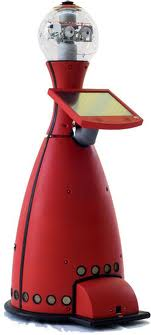
\includegraphics[width=0.3\linewidth]{scitosa5_1_model}
%	\vspace{4pt}
%	\captionof{figure}{The SCITOS-A5, mobile service robot by Metralabs GmbH \cite{Metralabs}}
%	\label{fig:scitosa5}
%\end{minipage}
%\qquad
%%%\begin{minipage}{0.4\textwidth}
%%%	\centering
%%%	\vspace{23pt}
%%%	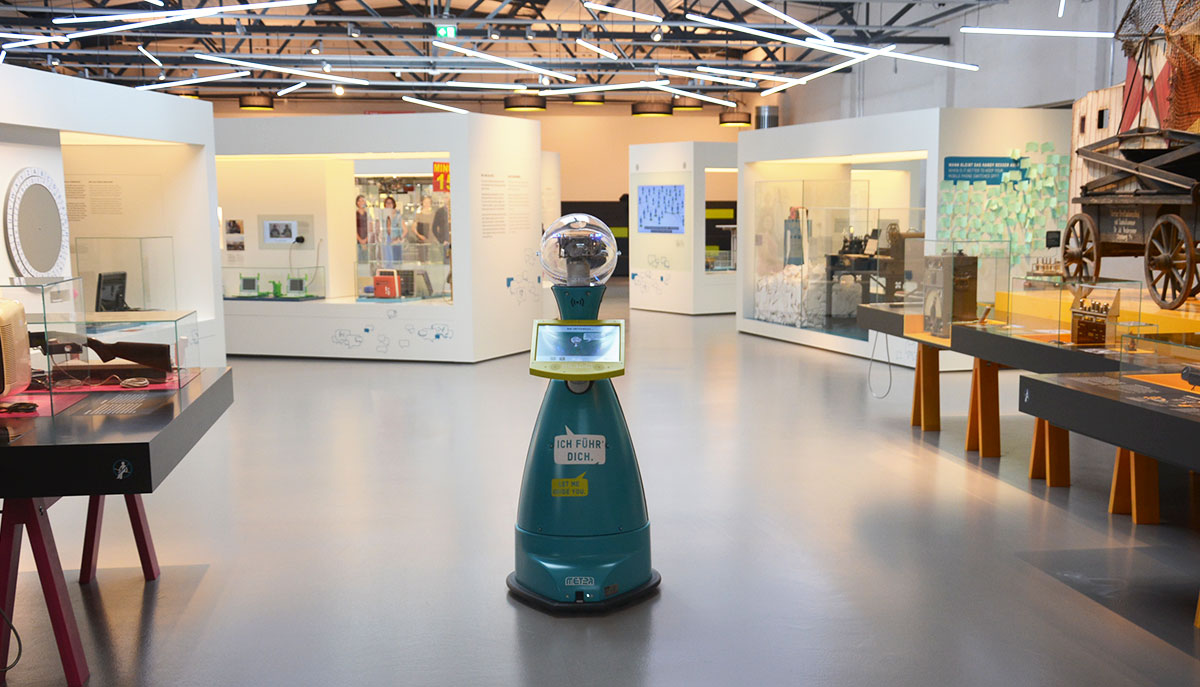
\includegraphics[width=1.1\linewidth]{scitosa5_2_TIM}
%%%	\vspace{-10pt}
%%%	\captionof{figure}{The SCITOS-A5 in one of its application environments. Shown here is robot \textit{TIM}, used for leading visitors of the German Technical Museum in Berlin through the exhibits \cite{Metralabs}.}
%%%	\label{fig:scitosa5_2}
%%%\end{minipage}
%\begin{minipage}{0.525\textwidth}
%	\centering
%	\vspace{10pt}
%	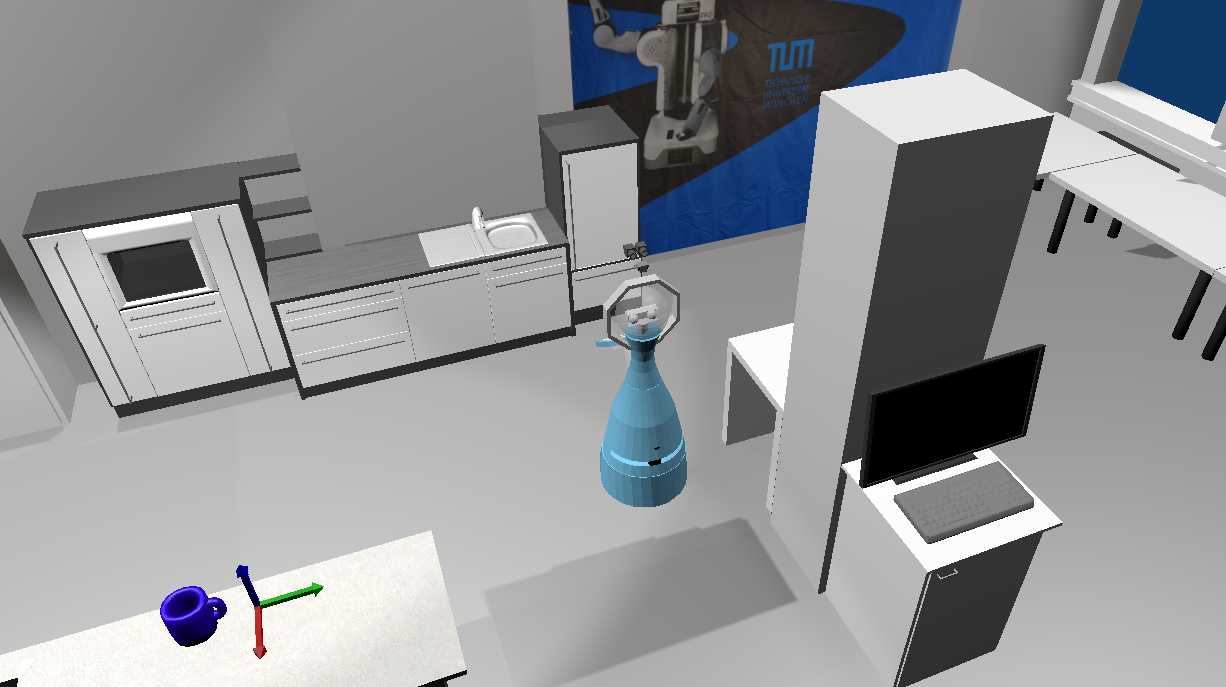
\includegraphics[width=1\linewidth]{simulator}
%	\vspace{-10pt}
%	\captionof{figure}{The SCITOS-A5 robot in a running MORSE simulation of the \texttt{tum\_kitchen} environment.}
%	\label{fig:simulator}
%\end{minipage}
%\quad
%\end{figure}

\begin{figure}[t]
	\centering
	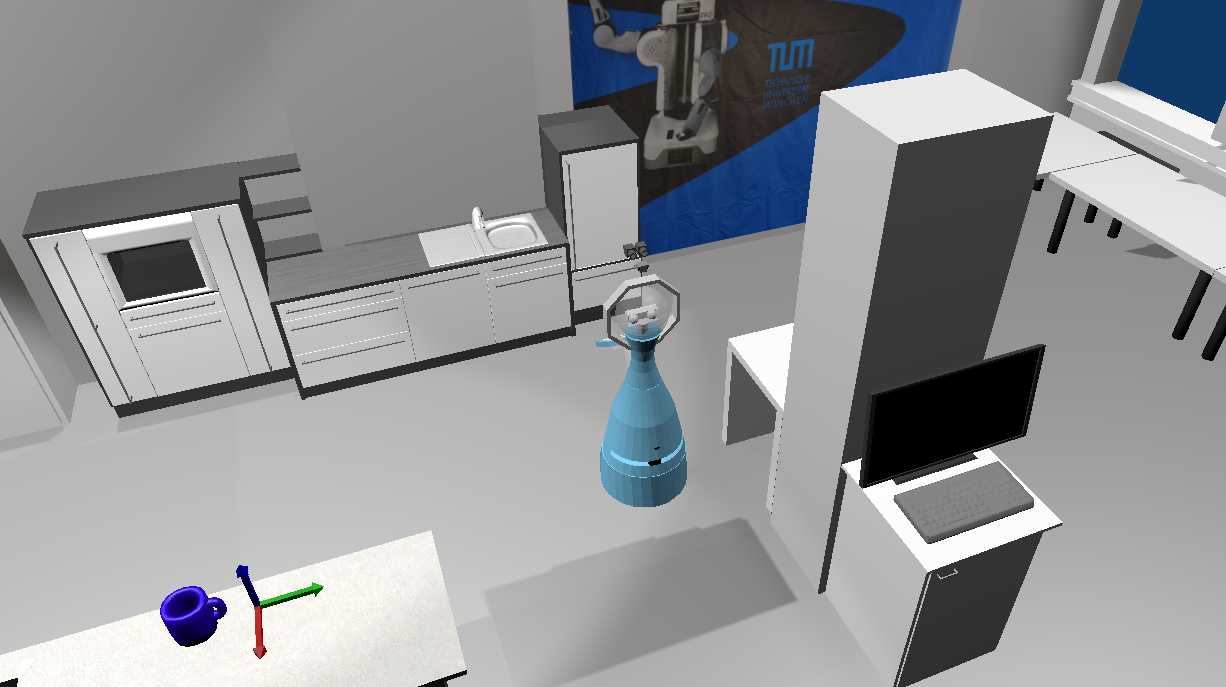
\includegraphics[width=0.65\linewidth]{simulator}
	\caption{The SCITOS-A5 mobile service robot in a running Morse simulation of the \texttt{tum\_kitchen} environment.}
	\label{fig:simulator}
\end{figure}

For performing simulations the \textit{MORSE} simulator \cite{morse_simpar_2012}, a generic simulator for academic robots, has been used in combination with the \textit{ROS} middleware to control the robot in an environment.
The simulations are performed with the Metralabs GmbH \textit{SCITOS-A5} \cite{Metralabs}, an industry-standard mobile service robot designed specifically for interacting with humans and guiding them to products or exhibits.
This robot is equipped with several sensors which can be used for navigation and \acrfull{acr:hri}, such as an omni-directional camera, 24 ultrasonic sensors, a collision sensor and a SICK laser range finder \cite{gross2008shopbot}.
As described in \autoref{sec:datasets} we are particularly interested in the odometric capabilities of the robot for the implementation that has been used in our experiments.
\autoref{fig:simulator} shows this robot in a MORSE simulation of one of the office environments used for our experiments.
The \texttt{strands-desktop} meta-package (developed as part of the \textit{STRANDS} project \cite{hawes2017strands}) was used to obtain all required simulation software mentioned above with ease, in which the environments used in the simulations of our experiments are contained as well.

%Software used for the implementation:
%\begin{itemize}
%	\item Programming Language: \textit{Python (2.7)} together with \texttt{scikit-learn}, \texttt{pymdptoolbox}, \texttt{bayesian-optimization} packages + explain what each of them are used for
%	\item Simulator: \textit{Morse}
%	\item Scitos-A5 robot, mobile service robot (plus \textit{short} discussion of what this robot has been used for in the real world)
%	\item Control movements of robot in simulator through \textit{ROS}
%\end{itemize}

\subsection{Dataset Acquisition}
\label{sec:datasets}

\begin{table}[pt]
	\caption{An excerpt of one of the execution traces datasets showing the format of the entries. Each entry stores the pose (\texttt{x}, \texttt{y} and \texttt{yaw}) of the robot based on odometry readings, and the action executed from this pose.}
	\label{tab:datasets-excerpt}\centering
	{\ttfamily
	\begin{tabular}{r|r|r|r}
		x & y & action\_id & yaw \\
		\hline
		2.243550300598145 & 3.1634166240692 & 1 & 0.7840424207077832 \\
		2.890618801116943 & 3.8128550052643 & 7 & -0.8159573629295891 \\
		3.541900634765625 & 3.1447956562042 & 6 & -1.6159579833378268 \\
		3.544688224792481 & 2.1472022533417 & 0 & -0.0326251734671011 \\
%		4.264401435852051 & 2.0662682056427 & 6 & -1.6326265827467716 \\
		... & ... & ... & ...
	\end{tabular}
	}
\end{table}

\begin{table}[pt]
	\caption{Details about the Morse simulation environments used and the size of the gathered datasets consisting of execution traces of the SCITOS-A5 robot.}
	\label{tab:datasets-environments}\centering
	\begin{tabular}{|l|r|r|}
		\hline
		\textbf{Environment Name} & \textbf{Approximate Area (\si{\metre\squared})} & \textbf{Number of Entries in Dataset} \\
		\hline
		\texttt{tum\_kitchen}& \num{100}              &   \num{4370}                                    \\
		\hline
		\texttt{uol\_bl}& \numrange[range-phrase = --]{800}{1000}               & \num{17245}           						\\ \hline          
	\end{tabular}
\end{table}

In order to be able to learn \acrshortpl{acr:mdp} from data and establish the optimization, we should obtain a dataset that  describes the environment the robot will operate in.
This dataset should describe possible robot poses and to what other poses the execution of the possible actions may lead to, in order to properly describe the dynamics of the system.

\newpage
For our implementation and the experiments that have been carried out, execution traces have been obtained by letting the robot follow a random action policy during which subsequent poses and actions are logged to a file.
This exploration is performed inside the simulator both for a relatively small environment (i.e., \texttt{tum\_kitchen}, based on a university kitchen of the Technical University of M\"unchen) and  large environment (i.e., \texttt{uol\_bl}, based on a floor in a faculty of the University of Lincoln) obtained from a repository of the \textit{STRANDS} project.

In the exploration a new entry is recorded in a file after each time-step of $t = \SI{1.0}{\second}$, which each contain the robot's pose based on odometric readings with its location as $x$ and $y$ position and its orientation described by the $yaw$.
Apart from that, each entry also stores the action that is executed next from the current pose.
As a result, the next entry tells us the robot's pose after the action in the previous entry has been executed.

In \autoref{tab:datasets-excerpt} an excerpt of one of the datasets is shown, which might give a clearer picture of the data that has been gathered and the format in which it has been stored.
The possible actions of the robot correspond to a discrete set of robot movements in $8$ different directions, being \textit{south}, \textit{south-east}, \textit{east}, \textit{north-east}, \textit{north}, \textit{north-west}, \textit{west} and \textit{south-west}.
For example, the first two entries describes the transformation of the robot's pose after trying to make a \textit{south-east} movement (n.b., positive difference in $x$ corresponds to moving south, while positive difference in $y$ corresponds to moving east).
\autoref{tab:datasets-environments} presents additional information about the environments and the size of the datasets gathered accordingly.

%Explain how the data-sets are obtained. 
%- For multiple environments - What is obtained. - How the data is obtained.

\subsection{Framework Implementation}
\label{sec:implementation}

To evaluate the framework proposed in \autoref{ch:methodology}, an implementation was made for the domain of mobile robot navigation.
This implementation optimizes for an \acrshort{acr:mdp} that maximizes the yielded performance of following plans derived from it. That is, it aims to find a model that ensures a mobile robot moves from one location in an environment to another as fast as possible.
In this section the relevant details of each part of the implementation are discussed.

\subsubsection{Learning Step}

For learning discrete-state \acrshortpl{acr:mdp} from the acquired execution traces, a likelihood maximization approach is applied based on a state space obtained from clustering algorithms.
That is, the state space is first obtained by applying a clustering algorithm (i.e., $k$-Means, \acrshort{acr:gmm}) with $\theta$ defining the number of components and the geometric positions of the execution traces as its training set.
Then, a transition probability distribution is fitted on the execution traces, such that an \acrshort{acr:mdp} may be obtained that comprehends the transitions that are possible when actions are performed from any of its states.

After having learned an \acrshort{acr:mdp}, the learning step next assesses the corresponding model value.
The model value is assessed based on how fast (i.e., expressed by the number of discrete time-steps) the agent would execute the tasks it is expected to perform when it is employed with the learned \acrshort{acr:mdp}.

For our domain we define each task as navigating from a start location to a goal location in the environment, each presented as a pair of coordinates, as fast as possible.
We translate these tasks into something that can be fed to the learned \acrshort{acr:mdp}, first of all, by setting the initial state of the \acrshort{acr:mdp} to the state predicted by the selected clustering algorithm for the start coordinates.
Similarly, a goal state is obtained, and accordingly a reward function for the \acrshort{acr:mdp} is defined as prescribed in \autoref{sec:learning-step}.
%by setting a one-time reward for this state.
%To avoid small state spaces (in which goal states do not map directly to true goals) yielding high value, a discrepancy factor is computed and used as described in \autoref{sec:learning-step}.

For each task, a value function and policy is computed for the \acrshort{acr:mdp} using the \acrshort{acr:vi} algorithm.
Based on the computed value functions and simulations following the corresponding policies, the value $V_\mathcal{M}$ of the learned \acrshort{acr:mdp} $\mathcal{M}$ is computed as in \autoref{eq:vm} of \autoref{sec:learning-step}.
In the simulations, for each task, the robot is first put at the start location defined by the task and then moves in the direction imposed by the computed policy at each discrete time-step.
It repeats this until the goal state has been reached.
At that point, however, the ``true'' goal might not have been reached by the robot.
This is a problem, because if we would quit the simulation as soon as the goal state has been reached, then \acrshortpl{acr:mdp} with state spaces that are too simple would yield high value.
To take this into account, as soon as the robot reaches the goal state, it checks if it is inside a designer-specified range of the goal location (i.e., the \textit{goal radius} in \autoref{tab:designer-settings}).
If not, the robot is moved into the direction of the goal location and the same check is performed.

To avoid the simulations running endlessly on a certain task, time-outs are defined at which the simulation is quit.
First of all, a (relatively short) \textit{goal time-out} is defined for reaching the goal from the goal state, which clearly cannot take too long.
Secondly, a \textit{stuck time-out} is defined, which starts when the robot remains at the same location after performing an action.
Finally, there is a \textit{global time-out}, that defines the maximum time the robot is allowed to spend on performing a task, taking into account any extra time caused by slipping.

The output of each learning step is the value of the learned model $V_\mathcal{M}$ and the time spent on model learning and planning.
The last being used when the \acrshort{acr:mei-ps} acquisition function is employed in the optimization.
Further, additional data is logged in each iteration, which is the total iteration time, simulation time, model learning time, total planning time and the parameter setting $\theta$ used.

%% IMPLEMENTATION LEARNING STEP
% Learning algorithm
	% Clustering algorithm
	% Maximum likelihood
% Objective: 
	% Learn MDP for given theta
	% Tasks (initial and goal locations)
	% Turned into reward function -> apply solver (VI) -> obtain value function and policy to use
	% Simulation:
		% Steps
		% Time-outs (1) stuck (2) goal state to reach goal (3) task
	% Output: Model value, time
% Logging

\begin{table}
	\caption{Settings for goal radius, parameter domain $\Theta$, time-outs and discount factor used for each of the environments in the experiments.}
	\label{tab:designer-settings}\centering
	\begin{tabular}{|l|r|r|r|r|r|r|}
		\hline
		\textbf{Environment} & \textbf{Goal Radius} & \textbf{Parameter} & \textbf{Goal T/O} & \textbf{Stuck T/O} & \textbf{Global T/O} & \textbf{Discount}  \\
		
		& \textbf{(\si\meter)} & \textbf{Domain $\Theta$} & (\si{\second}) & (\si{\second}) & (\si{\second}) & \textbf{Factor $\gamma$}\\
		\hline
		\texttt{tum\_kitchen} & \num{0.5} & $[2, 300]$ & \num{10} & \num{10} & \num{30} & \num{0.95} \\
		\hline
		\texttt{uol\_bl} & \num{1.0} & $[100, 1000]$ & \num{10} & \num{10} & \num{120} & \num{0.95}\\
		\hline
	\end{tabular}
\end{table}

\subsubsection{Optimization Step}

For the implementation of the framework for this domain we make use of the \acrshort{acr:bo} framework for optimization based on a \acrshort{acr:gp} with a Mat\'ern 3/2 kernel where the noise in the simulations is approximated by adding Gaussian white noise through a White kernel with estimated noise~level of $10^{-4}$.
As initially there is no knowledge about the model value given a parameter setting $\theta$, first, a number of random settings are selected for which yielded performance is assessed and stored in an evidence set.
In the following iterations new settings for $\theta$ are chosen with maximum utility in the selected acquisition function, which is repeated for a fixed number of iterations.

The first phase of the multi-phase framework described in \autoref{sec:multi-phase-framework} is executed as an individual optimization procedure, where the model values $V_\mathcal{M}$ are solely based on computed value functions and no simulations are performed.
The resulting posterior of this first phase is then used in the acquisition of the first few samples in the second phase with the aim of finding a global maximizer faster.

%% OPTIMIZATION STEP
% Initial points (random points)
% Stopping criterions


%Details on the implementation; how the framework/routine is implemented for this application. Discuss how the following aspects are taken care of in the implementation:
%\begin{itemize}
%	\item Environments
%	\item Exploration / Data Gathering
%	\item Optimization
%	\item Simulations of following policy
%\end{itemize}

\afterpage{
	\begin{figure}
		\centering
		%\captionsetup{font=small}
		\captionsetup[subfigure]{font=footnotesize}
		%\captionsetup[subfigure]{justification=centering}
		\begin{subfigure}{\textwidth}
			\centering
			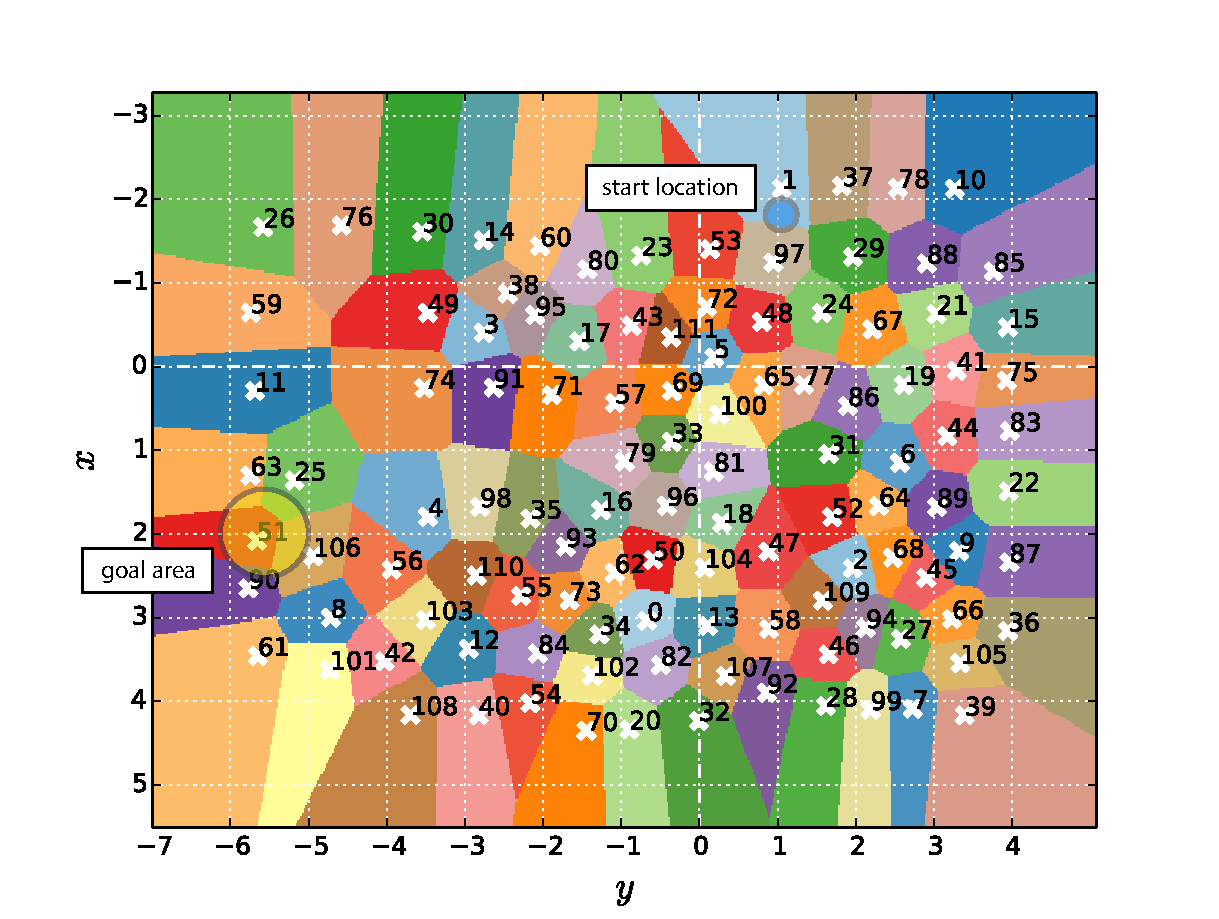
\includegraphics[width=\linewidth]{demo_clustering_v2}
			\caption{State space of an \acrshort{acr:mdp} with $112$ states for the \texttt{tum\_kitchen} environment learned by $k$-Means clustering. The plot depicts one of the tasks the mobile robot is expected to perform. The start location maps to a single state, labeled `$\mathsf{1}$'. The goal center maps to the state labeled `$\mathsf{51}$', while the goal area intersects with multiple states.}
			\label{fig:demo-clustering}
		\end{subfigure}
		
		\bigskip
		
		\begin{subfigure}{\textwidth}
			\centering
			%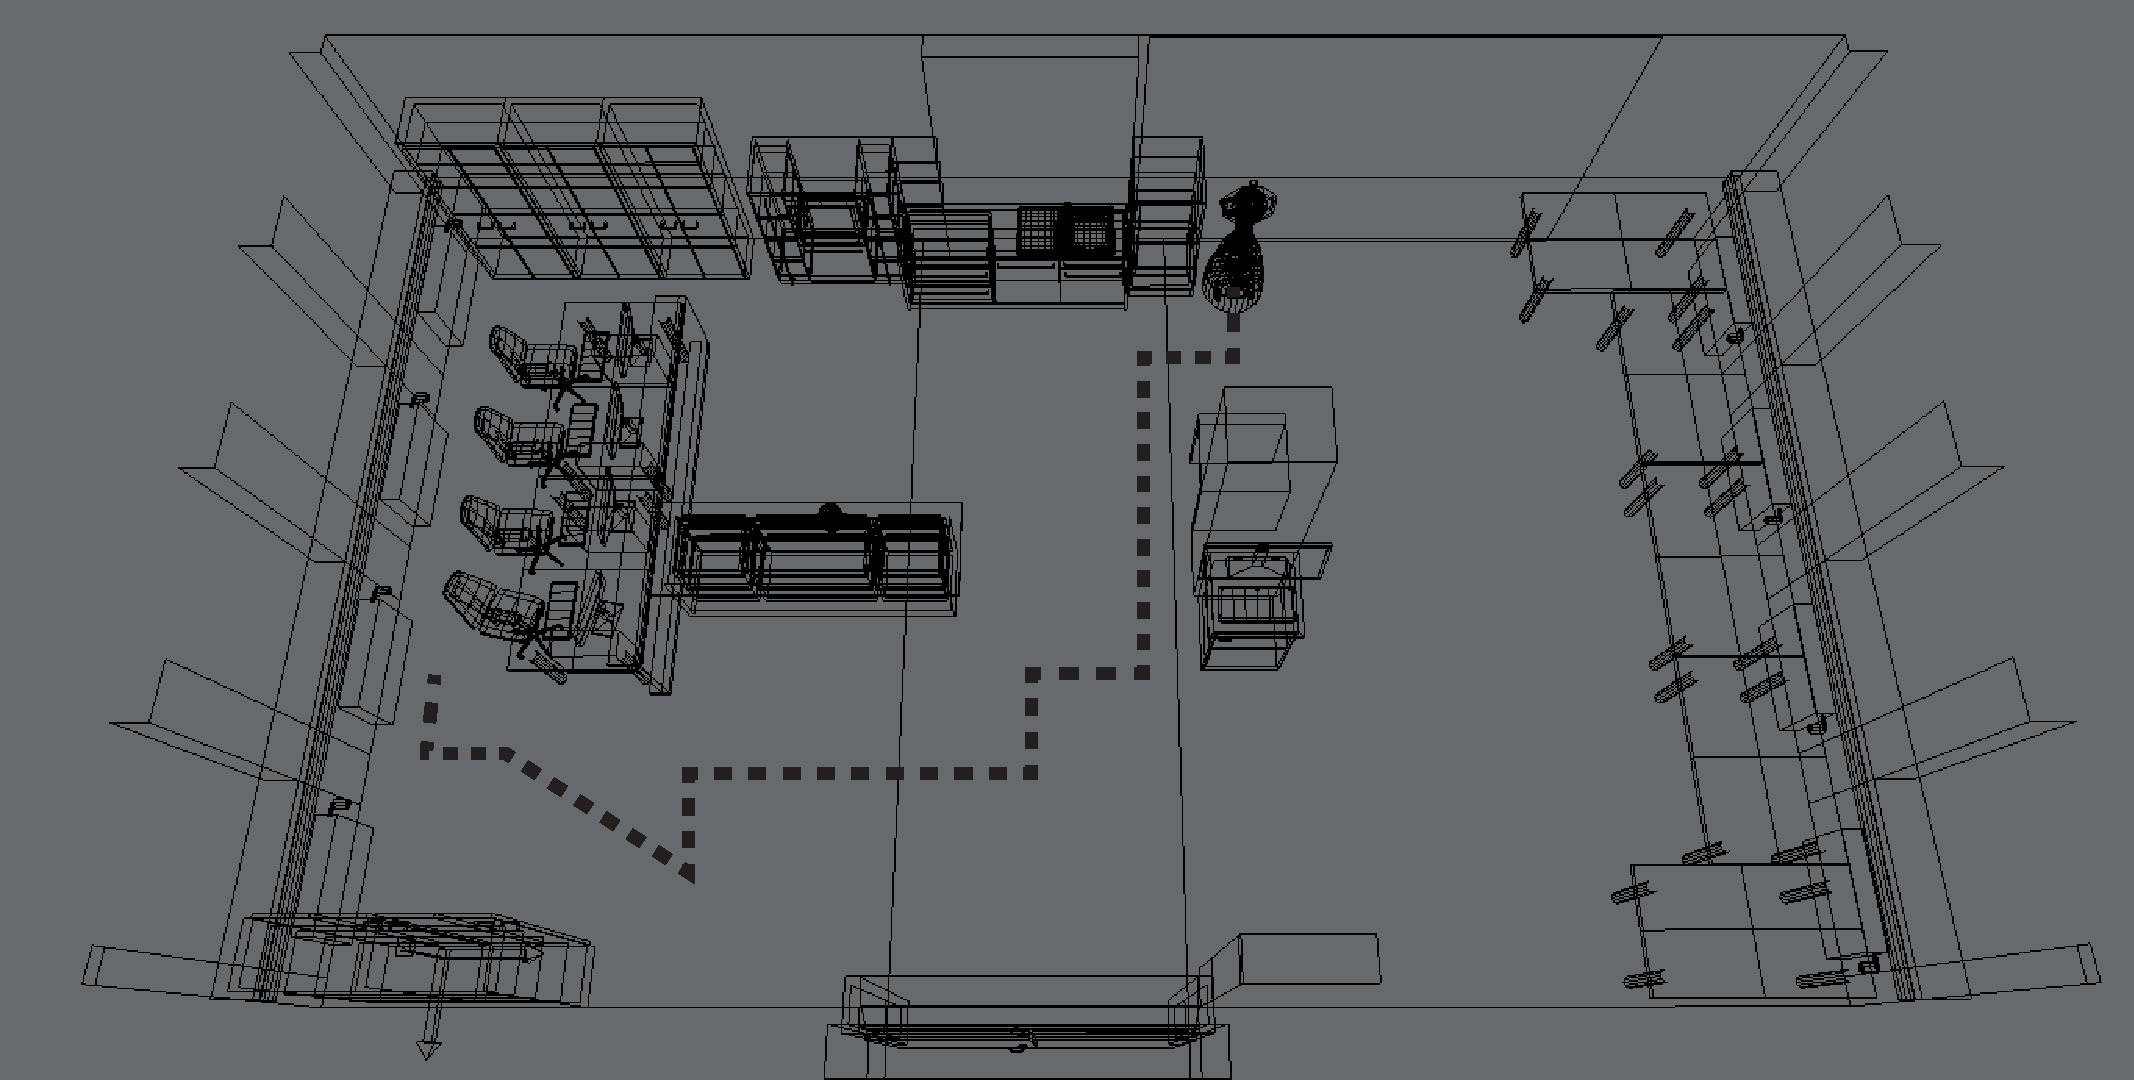
\includegraphics[width=\linewidth]{trajectory_v4}
			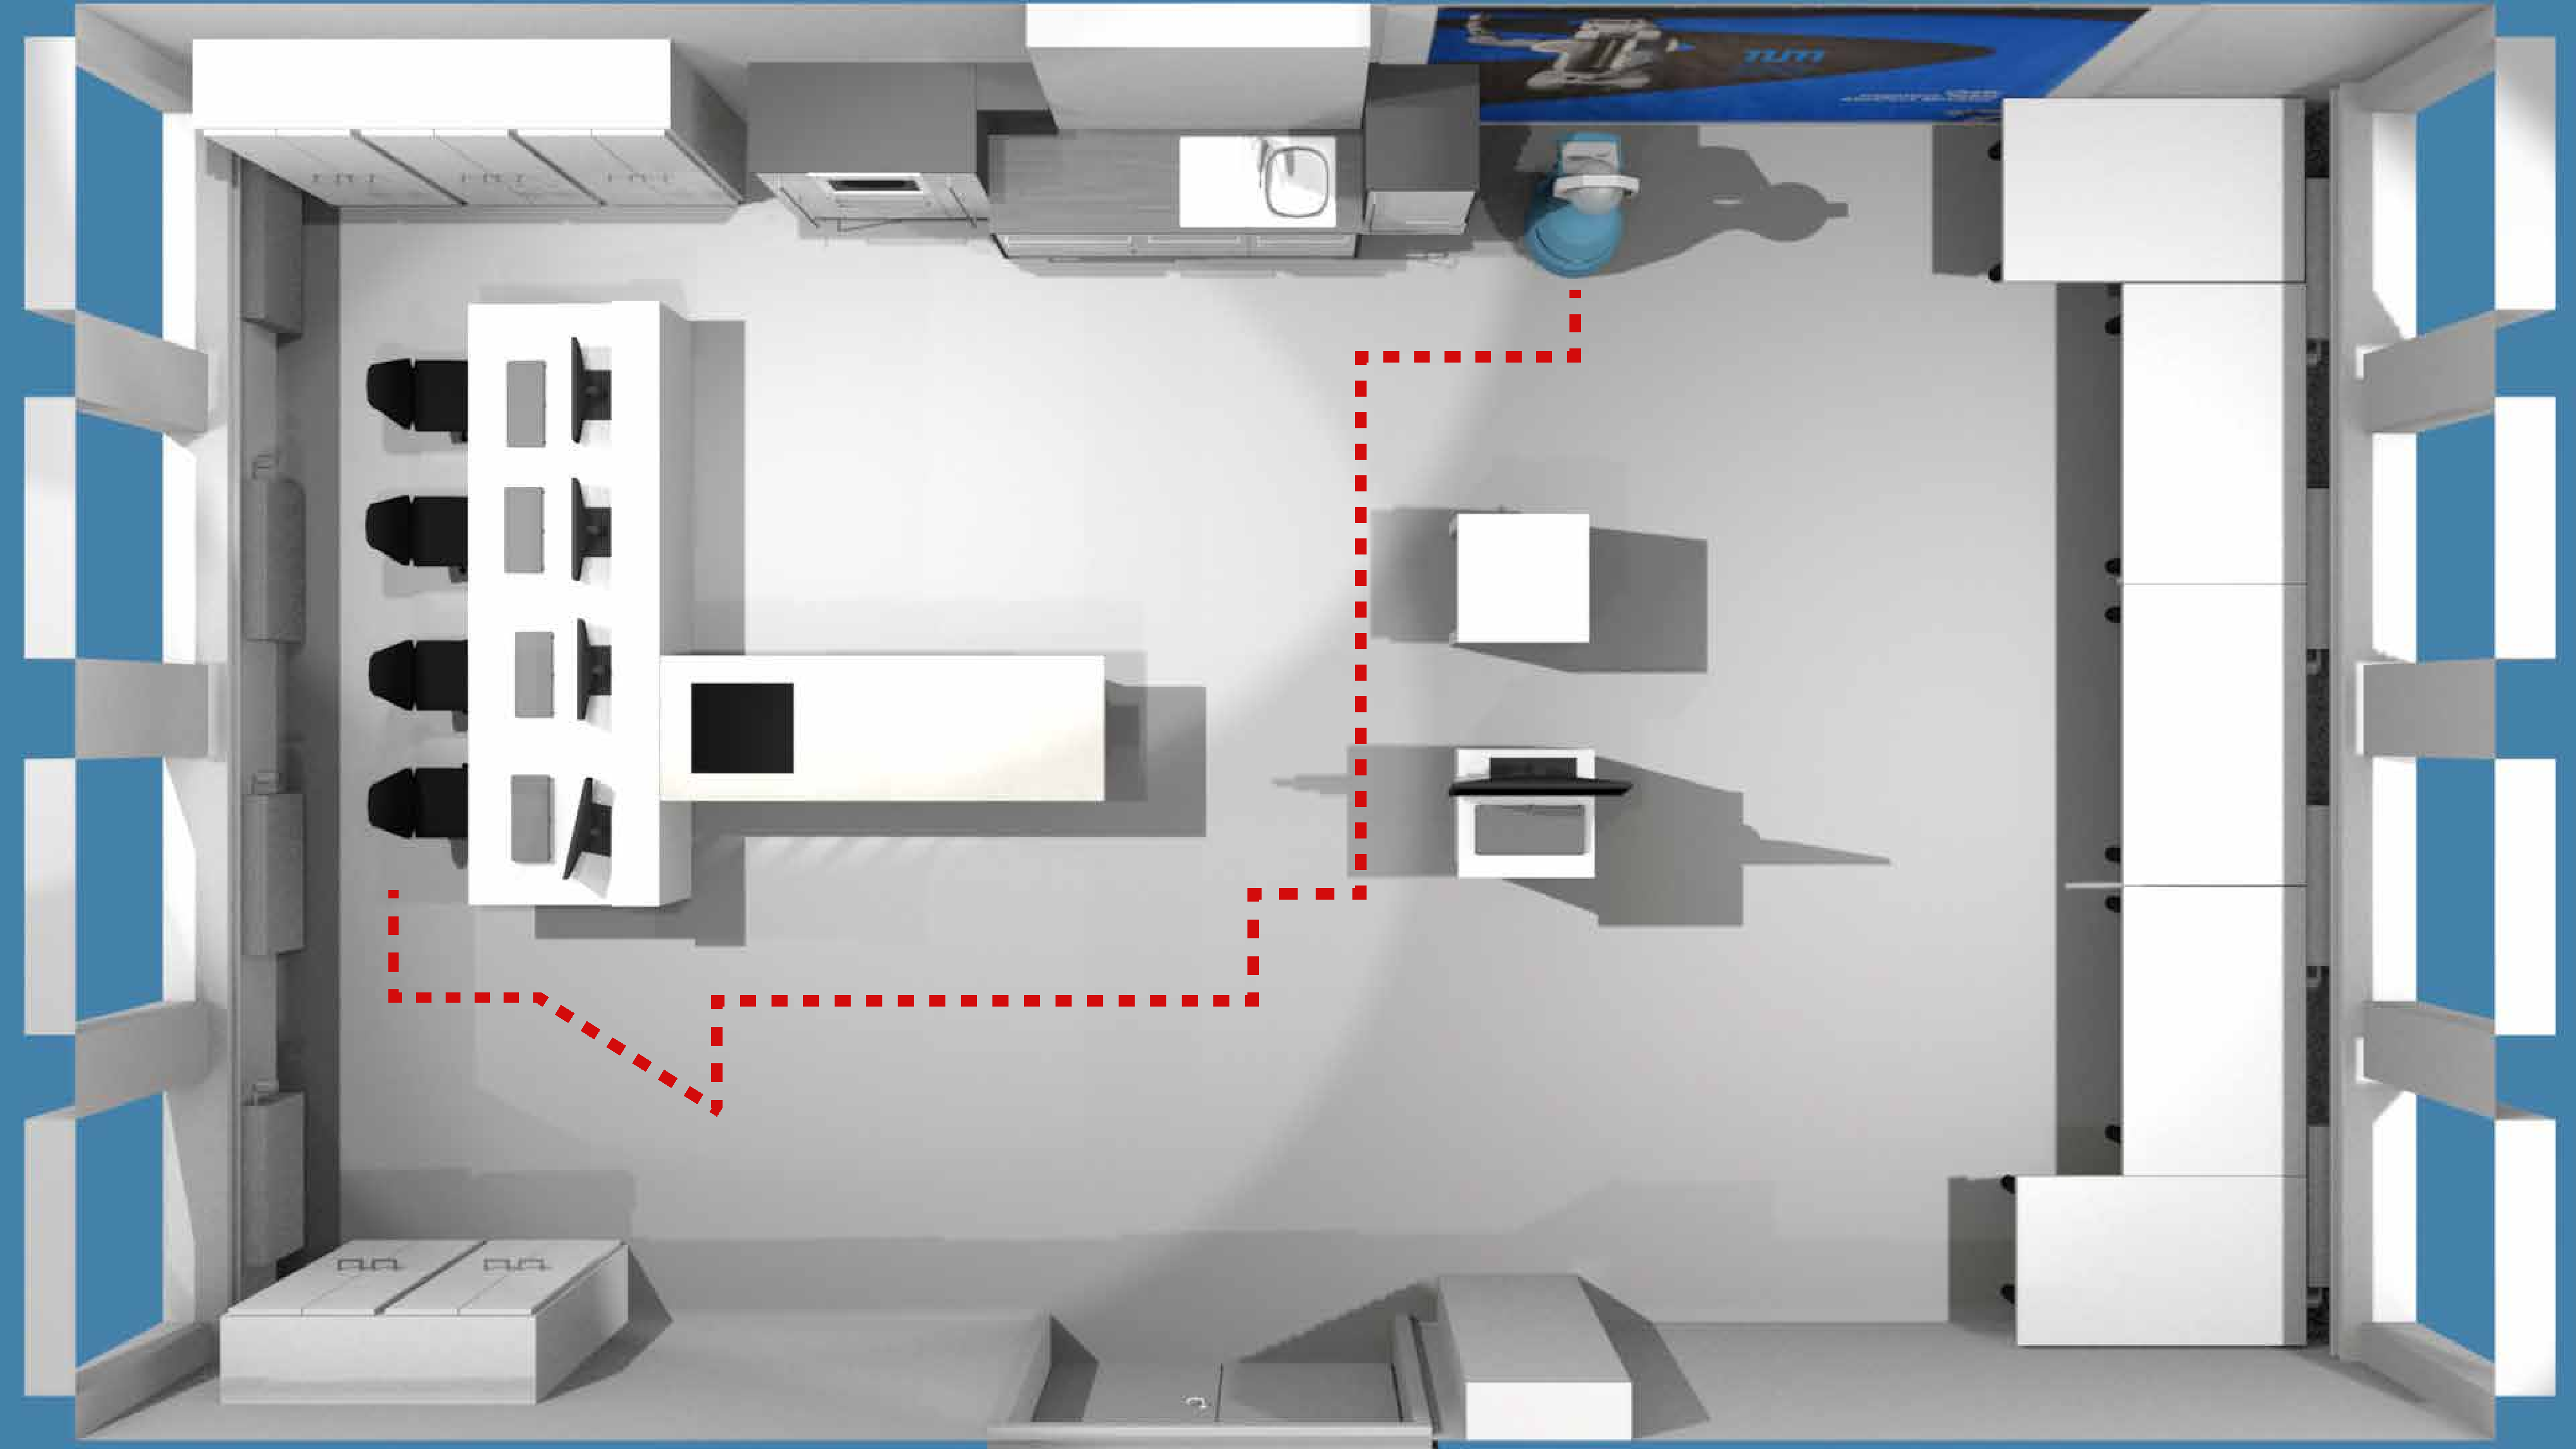
\includegraphics[width=\linewidth]{tum_kitchen_render_trajectory_v5_2}
			\caption{A MORSE simulation of the \texttt{tum\_kitchen} environment, showing the trajectory the SCITOS-A5 robot will follow to accomplish the task depicted in \autoref{fig:demo-clustering} according to the policy computed from the \acrshort{acr:mdp} using the \acrshort{acr:vi} algorithm.}
			\label{fig:demo-trajectory}
		\end{subfigure}
		\bigskip
		
		\caption{Demonstration of the implementation learning the state space of an \acrshort{acr:mdp} and using it for path planning for a task in the \texttt{tum\_kitchen} environment.}
		\label{fig:demonstration}
	\end{figure}
	\clearpage
}

\newpage

\subsection{Demonstration}
\label{sec:demonstration}

To provide the reader with a better insight as to how the implementation utilizes execution traces to learn \acrshortpl{acr:mdp} and use these for path planning, a demonstration is given of a single iteration of the framework, supported by the illustrations in \autoref{fig:demonstration}.
For this demonstration, let us assume that the optimization step provides us with a new parameter setting $\theta = 112$, specifying the number of states of the \acrshort{acr:mdp}, to evaluate.

First, given this parameter setting, a state space $\mathcal{S}$ is, in this case, learned by a $k$-Means clustering on the execution traces $E$, with the result shown in \autoref{fig:demo-clustering}.
Correspondingly, the transition function $\delta$ is fitted by maximum likelihood and a set of tasks $T$ are mapped to this state space.
To illustrate, let us take the task of moving from the position $(-1.9, 1.05)$ to $(2.0, -5.6)$, mapping to the states labeled with `$\mathsf{1}$' and `$\mathsf{51}$' respectively as shown in \autoref{fig:demo-clustering}.
Translating this into an initial state $s_0$ and reward function $R$, as described in \autoref{sec:learning-step}, results in an \acrshort{acr:mdp} $(\mathcal{S}, s_0, A, \delta, R)$ that can be solved using the \acrshort{acr:vi} algorithm to obtain a policy (and value function).
Then, to assess the performance in the simulator, this policy is employed, so that the robot will follow the trajectory as shown in \autoref{fig:demo-trajectory} (n.b., additionally, the robot might slip, so that it slightly deviates from this path).
Then, with $n$ being the recorded total number of time-steps, a performance measure for this task is obtained through \autoref{eq:vsim}.

%\begin{figure}[t!]
%	\centering
%	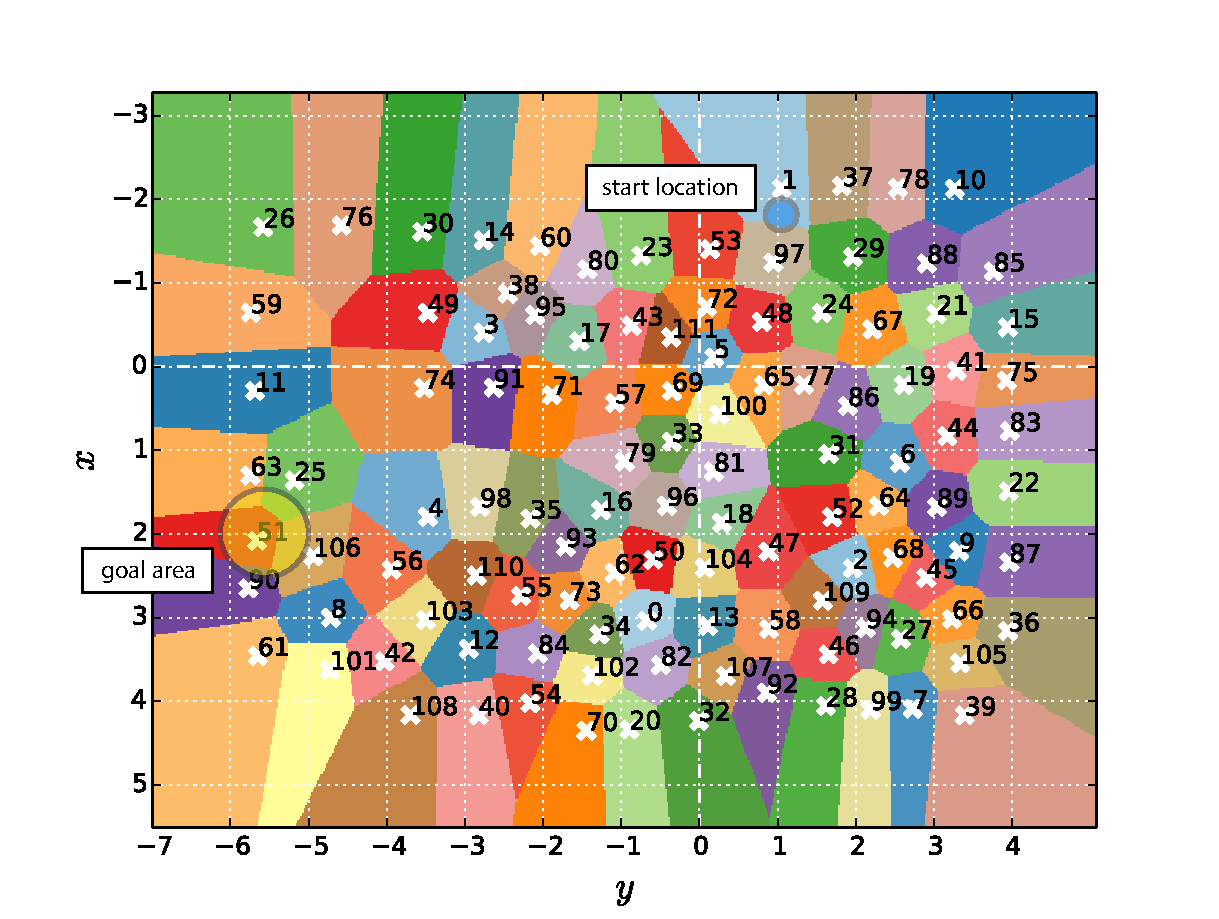
\includegraphics[width=0.9\textwidth]{demo_clustering_v2}
%	\caption{Clustering}
%	\label{fig:demo-clustering}
%\end{figure}
%
%\begin{figure}[t!]
%		\centering
%		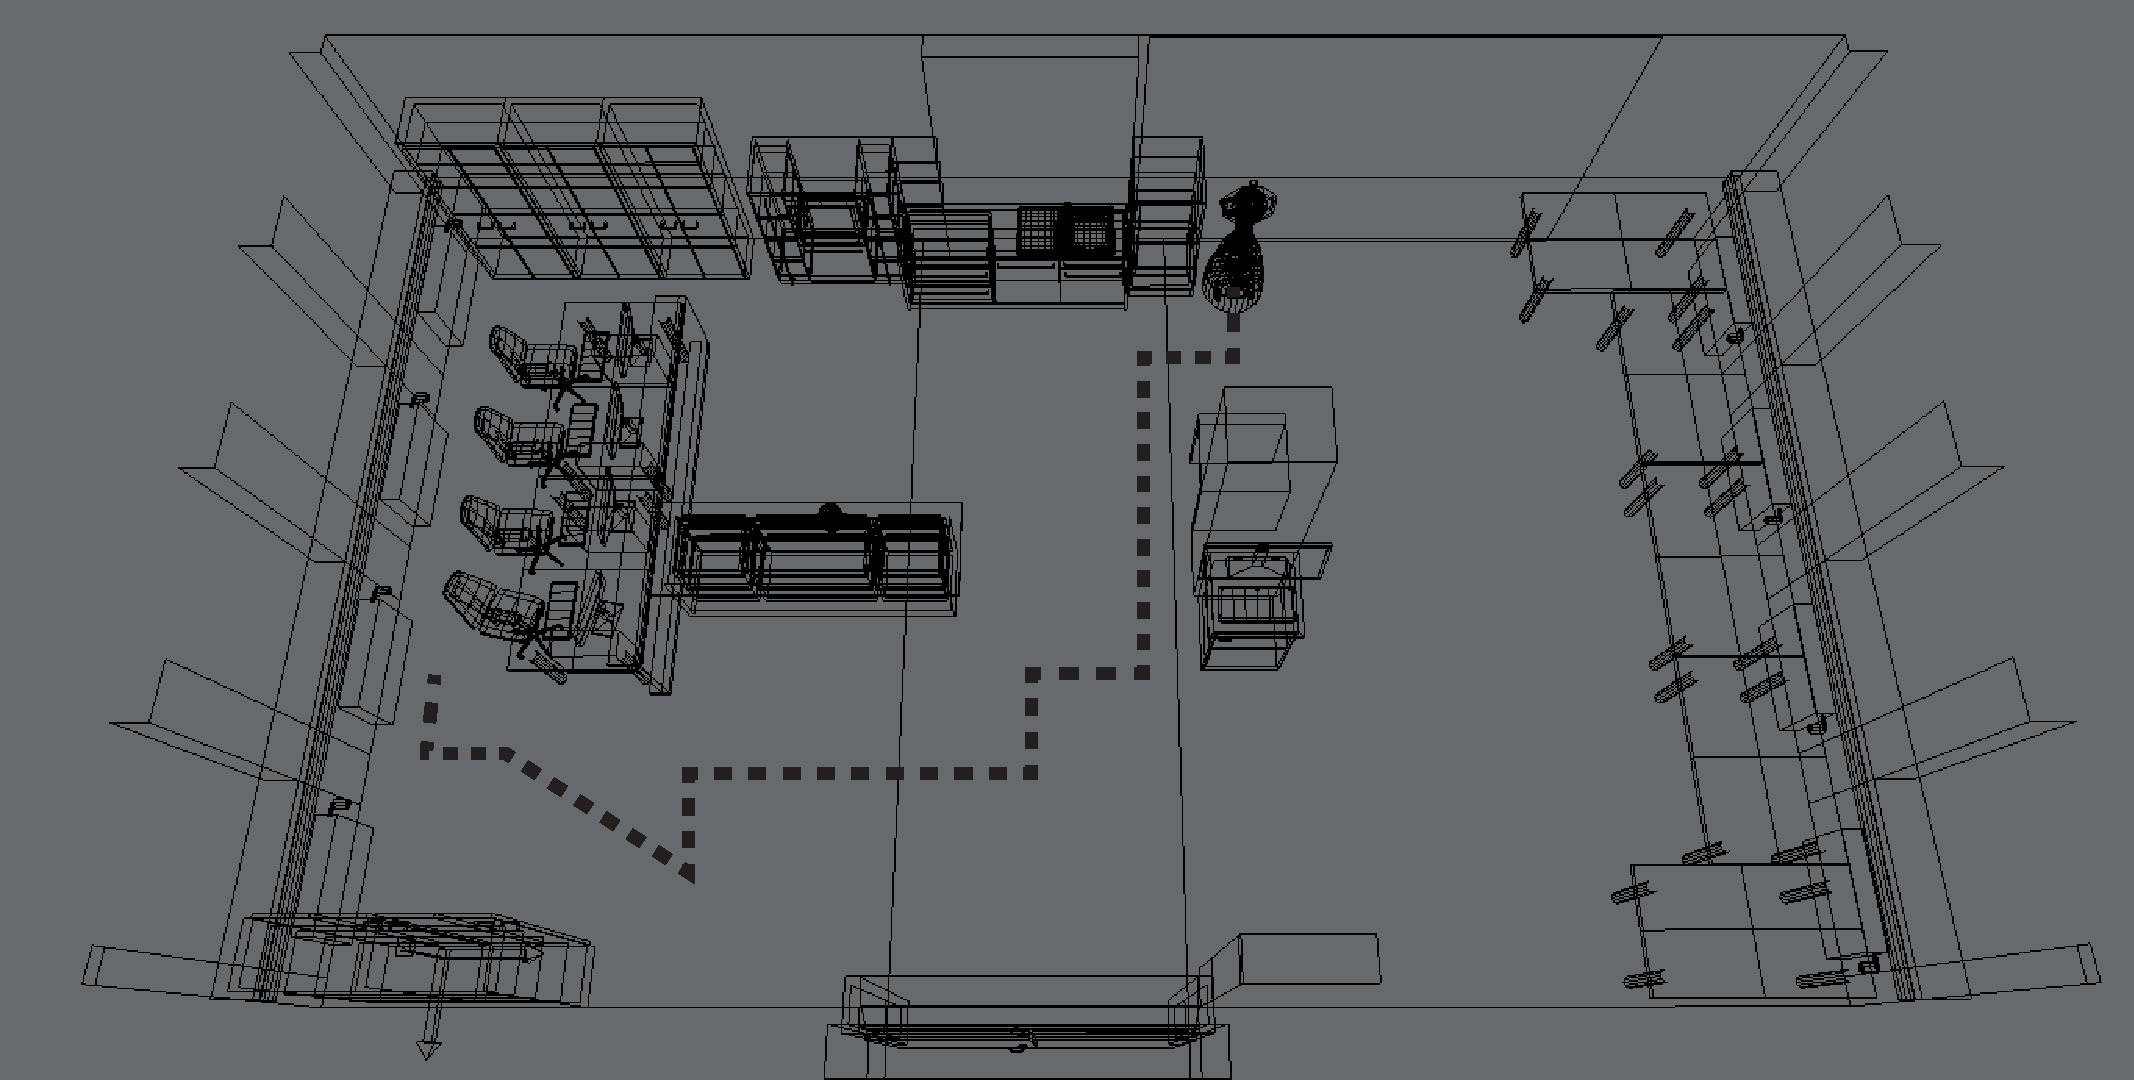
\includegraphics[width=\linewidth]{trajectory_v4}
%		\caption{Trajectory.}
%		\label{fig:demo-trajectory}
%\end{figure}

%\newpage

\section{Experiment Configurations}
\label{sec:scenarios}

\begin{table}[t!]
	\caption{Details on the different configurations used for the experiments on the base (single phase) framework.}
	\label{tab:configurations-base}\centering
	\begin{tabular}{|l|l|r|l|l|r|}
		\hline
		\textbf{ID} & \textbf{Environment} & \textbf{Weight Factor $\beta$} & \textbf{Acquisition Function} & \textbf{Algorithm} & \textbf{Dataset Used} \\
		\hline 
		1 & \texttt{tum\_kitchen} & 0.0 & \acrshort{acr:mei} & $k$-Means & 100\% \\
		\hline
		2 & \texttt{tum\_kitchen} & 0.0 & \acrshort{acr:mei} & $k$-Means & 75\%  \\
		\hline
		3 & \texttt{tum\_kitchen} & 0.0 & \acrshort{acr:mei} & $k$-Means & 50\% \\
		\hline
		4 & \texttt{tum\_kitchen} & 0.0 & \acrshort{acr:gp-ucb} & $k$-Means & 100\% \\
		\hline
		5 & \texttt{tum\_kitchen} & 0.0 & \acrshort{acr:mei-ps} & $k$-Means & 100\% \\
		\hline
		6 & \texttt{tum\_kitchen} & 0.0 & \acrshort{acr:mei} & \acrshort{acr:gmm} & 100\% \\
		\hline
		7 & \texttt{tum\_kitchen} & 0.0 & \acrshort{acr:gp-ucb} & \acrshort{acr:gmm} & 100\% \\
		\hline
		%6 & \texttt{tum\_kitchen} & 0.0 & \acrshort{acr:gp-ucb} & \acrshort{acr:gmm} & 100\% \\
		%\hline
		8 & \texttt{tum\_kitchen} & 0.25 & \acrshort{acr:mei} & $k$-Means & 100\% \\
		\hline
		9 & \texttt{tum\_kitchen} & 0.50 & \acrshort{acr:mei} & $k$-Means & 100\% \\
		\hline
		10 & \texttt{uol\_bl} & 0.0 & \acrshort{acr:mei} & $k$-Means & 100\% \\
		\hline
		%10 & \texttt{uol\_bl} & 0.0 & \acrshort{acr:mei} & $k$-Means & 75\%  \\
		%\hline
		%11 & \texttt{uol\_bl} & 0.0 & \acrshort{acr:mei} & $k$-Means & 50\% \\
		%\hline
		%12 & \texttt{uol\_bl} & 0.0 & \acrshort{acr:mei} & \acrshort{acr:gmm} & 100\% \\
		%\hline
		11 & \texttt{uol\_bl} & 0.0 & \acrshort{acr:gp-ucb} & $k$-Means & 100\% \\
		\hline
		12 & \texttt{uol\_bl} & 0.0 & \acrshort{acr:mei-ps} & $k$-Means & 100\% \\
		\hline
		%14 & \texttt{uol\_bl} & 0.0 & \acrshort{acr:gp-ucb} & \acrshort{acr:gmm} & 100\% \\
		%\hline
		%15 & \texttt{uol\_bl} & 0.25 & \acrshort{acr:mei} & $k$-Means & 100\% \\
		%\hline
		%16 & \texttt{uol\_bl} & 0.50 & \acrshort{acr:mei} & $k$-Means & 100\% \\
		%\hline
	\end{tabular}
\end{table}

\begin{table}[t!]
	\caption{Details on the different configurations used for the experiments on the multi-phase framework.}
	\label{tab:configurations-multi}\centering
	\begin{tabular}{|l|l|r|l|l|r|}
		\hline
		\textbf{ID} & \textbf{Environment} & \textbf{Weight Factor $\beta$} & \textbf{Acquisition Function} & \textbf{Algorithm} & \textbf{Dataset Used} \\
		\hline 
		13 & \texttt{tum\_kitchen} & 0.0 & \acrshort{acr:mei} & $k$-Means & 100\% \\
		\hline
		14 & \texttt{tum\_kitchen} & 0.0 & \acrshort{acr:gp-ucb} & $k$-Means & 100\% \\
		\hline
%		15 & \texttt{tum\_kitchen} & 0.50 & \acrshort{acr:mei} & $k$-Means & 100\% \\
%		\hline
		15 & \texttt{uol\_bl} & 0.0 & \acrshort{acr:mei} & $k$-Means & 100\% \\
		\hline
		16 & \texttt{uol\_bl} & 0.0 & \acrshort{acr:gp-ucb} & $k$-Means & 100\% \\
		\hline
%		17 & \texttt{uol\_bl} & 0.25 & \acrshort{acr:mei} & $k$-Means & 100\% \\
%		\hline
%		18 & \texttt{uol\_bl} & 0.50 & \acrshort{acr:mei} & $k$-Means & 100\% \\
%		\hline
	\end{tabular}
\end{table}

In this section an overview is provided of the experiments that have been performed with the robot navigation implementation of the framework.
\autoref{tab:designer-settings} shows the auxiliary settings used in the experiments for aspects like time-outs, parameter domain and goal radius for each of the environments.
Experiments are conducted for both the \textit{base} framework and \textit{multi-phase} framework with each of the environments.
The configurations for these experiments are shown in \autoref{tab:configurations-base} and \autoref{tab:configurations-multi} respectively.

The configurations were chosen with the aim of being able to identify how the results are affected based on changes in the used acquisition function, weight factor, clustering algorithm and the part of the dataset used.
In each of these experiments data is stored that comprise the generated evidence sets, log-files and the \acrshortpl{acr:mdp} that yield the best performance.
In the next section the obtained results for each of these configurations are shown and discussed accordingly.

%Discuss the different configurations that are to be compared
%\begin{itemize}
%	\item Fixed values for $\beta$-parameter vs. gradually decreasing from $1$ to $0$
%	\item Multiple environments: small (\texttt{tum\_kitchen}); large (\texttt{uol\_bl})
%	\item Model-learning algorithms: direct clustering vs. trajectory clustering; $k$-means vs. GMM
%	\item Data-sets of different sizes
%\end{itemize}

%\noindent Configurations for the basic optimization framework (only based on simulations):
%\begin{itemize}
%	\item Fixed value for $\beta$ (i.e., which weighs $V_\mathit{DTP}$): $0$, $0.25$ and $0.5$
%	\item Acquisition functions: \acrshort{acr:gp-ucb}, \acrshort{acr:mei}
%	\item GMM vs. $k$-Means (vs. trajectory clustering if time available)
%	\item All available data, 75\% and 50\%
%	\item Discount factor: $\gamma = 0.95$
%	\item Small environment: \texttt{tum\_kitchen}; and large environment: \texttt{uol\_bl}
%\end{itemize}
%We need to record: number of iterations, total time passed, optimum found ($\theta_\textnormal{max}$ and $V_{\mathcal{M},\textnormal{max}}$)
%
%\vspace{12pt}
%\noindent For the cost-incremental extension we could try to observe what happens when we decrease $\beta$ gradually over time.
%
%\vspace{12pt}
%\noindent Do we want to do something with `variable resolution' as post-processing step in the experiments?
%
%\vspace{12pt}
%\noindent\fbox{\textbf{TODO:} Table to be added describing the configurations/scenarios for the experiments.}

\section{Results and Discussion}
\label{sec:results}
%vTODO Fix order of figures and update text

From the experiments that have been performed according to the configurations presented in \autoref{sec:scenarios} results have been obtained that are discussed in this section.
First, we present and review the results obtained for the experiments that follow the base framework in \autoref{sec:base-framework-results}.
Then, in \autoref{sec:multiphase-framework-results} the results for the multi-phase extension of the framework are presented and discussed. 
Each of the figures in these sections present plots for each of the experiments, showing the resulting posterior from the gathered evidence, and the value~$V_\mathcal{M}$ of the learned model in each iteration of the \acrshort{acr:bo} optimization process.
%In these plots $\theta$ is the parameter-setting for model learning and $f$ is the (unknown) objective function mapping these to model values.

\subsection{Base Framework}
\label{sec:base-framework-results}

First off, we present and evaluate the results obtained from the experiments on the base framework.
As shown in \autoref{tab:configurations-base}, experiments have been performed on two different simulation environments: the small \texttt{tum\_kitchen} environment and the, in comparison, large \texttt{uol\_bl} environment, for which the results are discussed in the following sections.

\begin{figure}[t]
	\centering
	\captionsetup{font=small}
	\captionsetup[subfigure]{font=footnotesize}
	\captionsetup[subfigure]{justification=centering}
	\begin{subfigure}[t]{0.495\textwidth}
		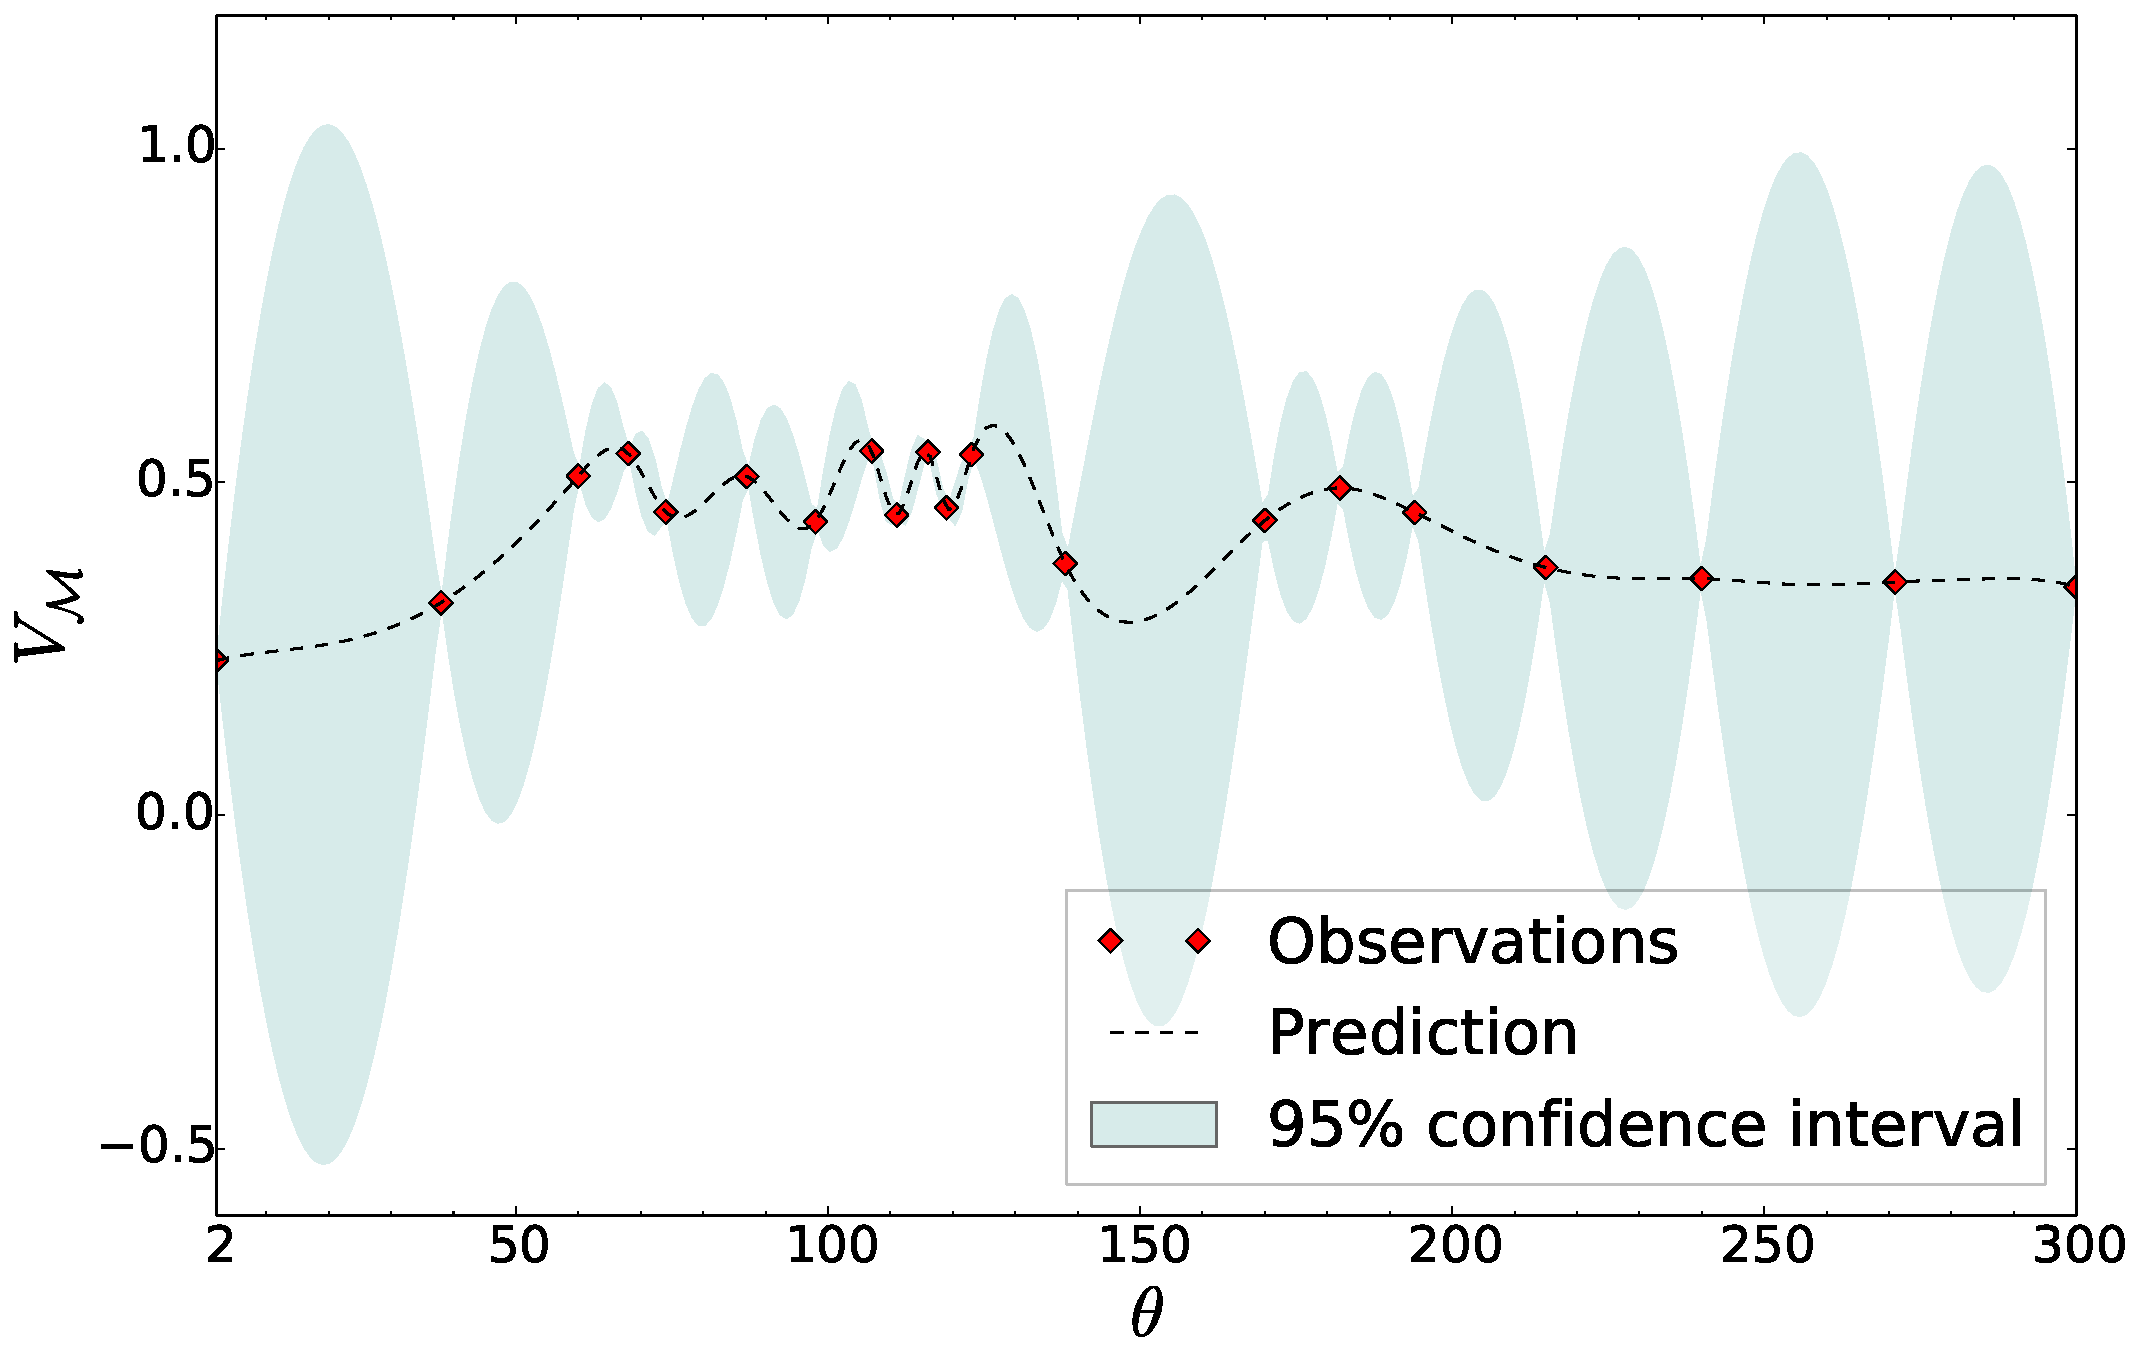
\includegraphics[width=\textwidth]{plots/tum_base/plot_b_00__alg_kmeans_pct_100_acq_ei}
		\caption{Experiment 1: 100\% of the dataset used}
		\label{fig:exp1}
	\end{subfigure}
	\begin{subfigure}[t]{0.495\textwidth}
		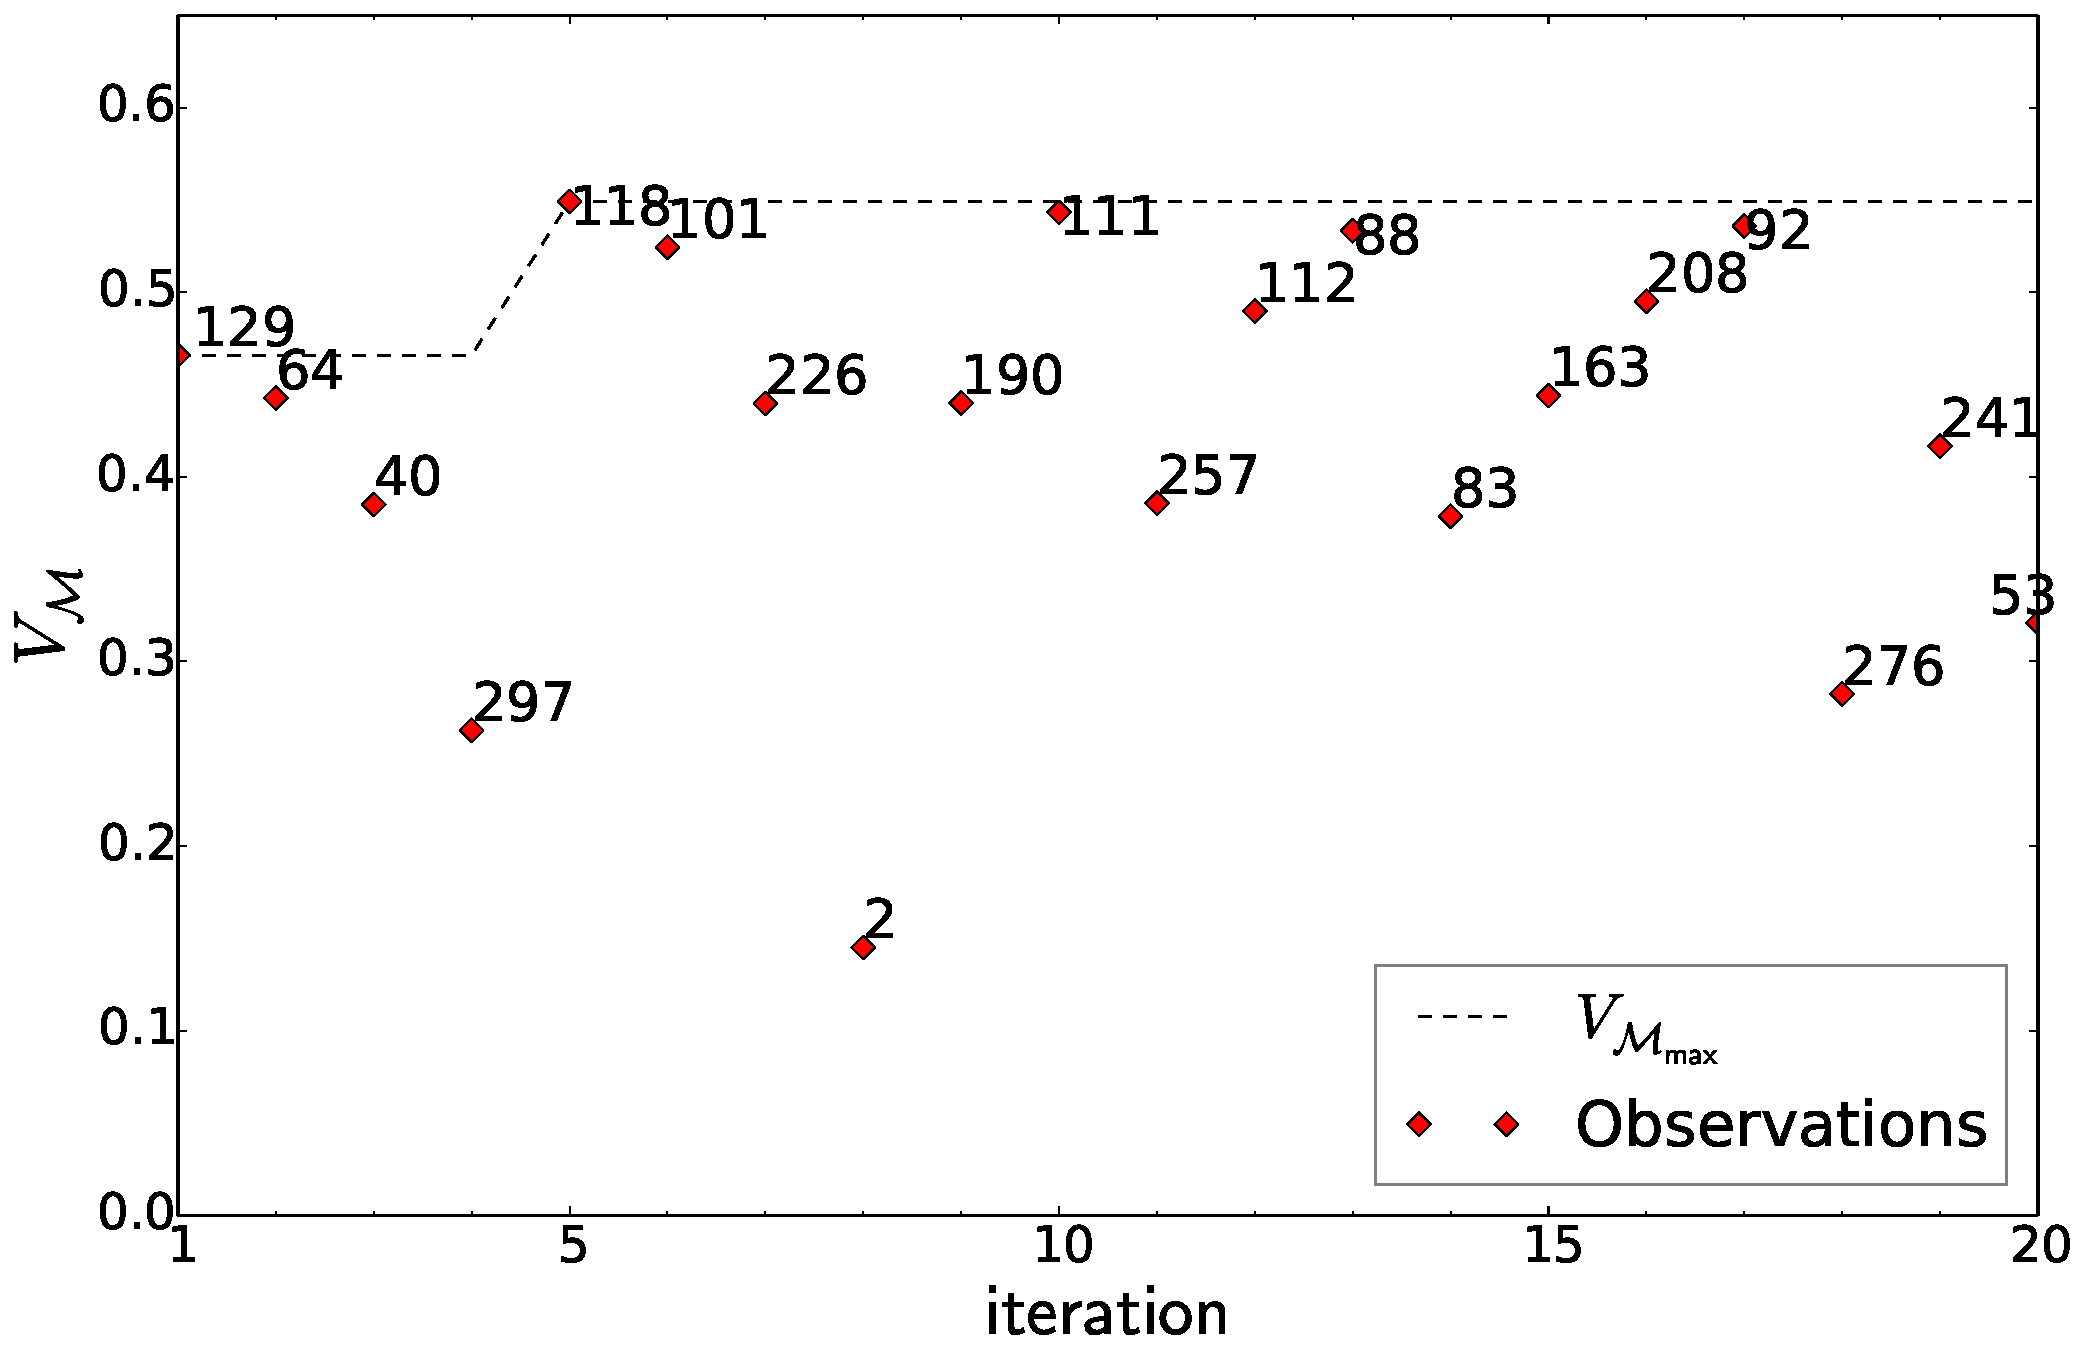
\includegraphics[width=\textwidth]{plots/tum_base/plot_b_00__alg_kmeans_pct_100_acq_ei_maximum_2}
		\caption{Experiment 1: Observations over iterations}
		\label{fig:exp1_observations}
	\end{subfigure}
	\begin{subfigure}[t]{0.495\textwidth}
		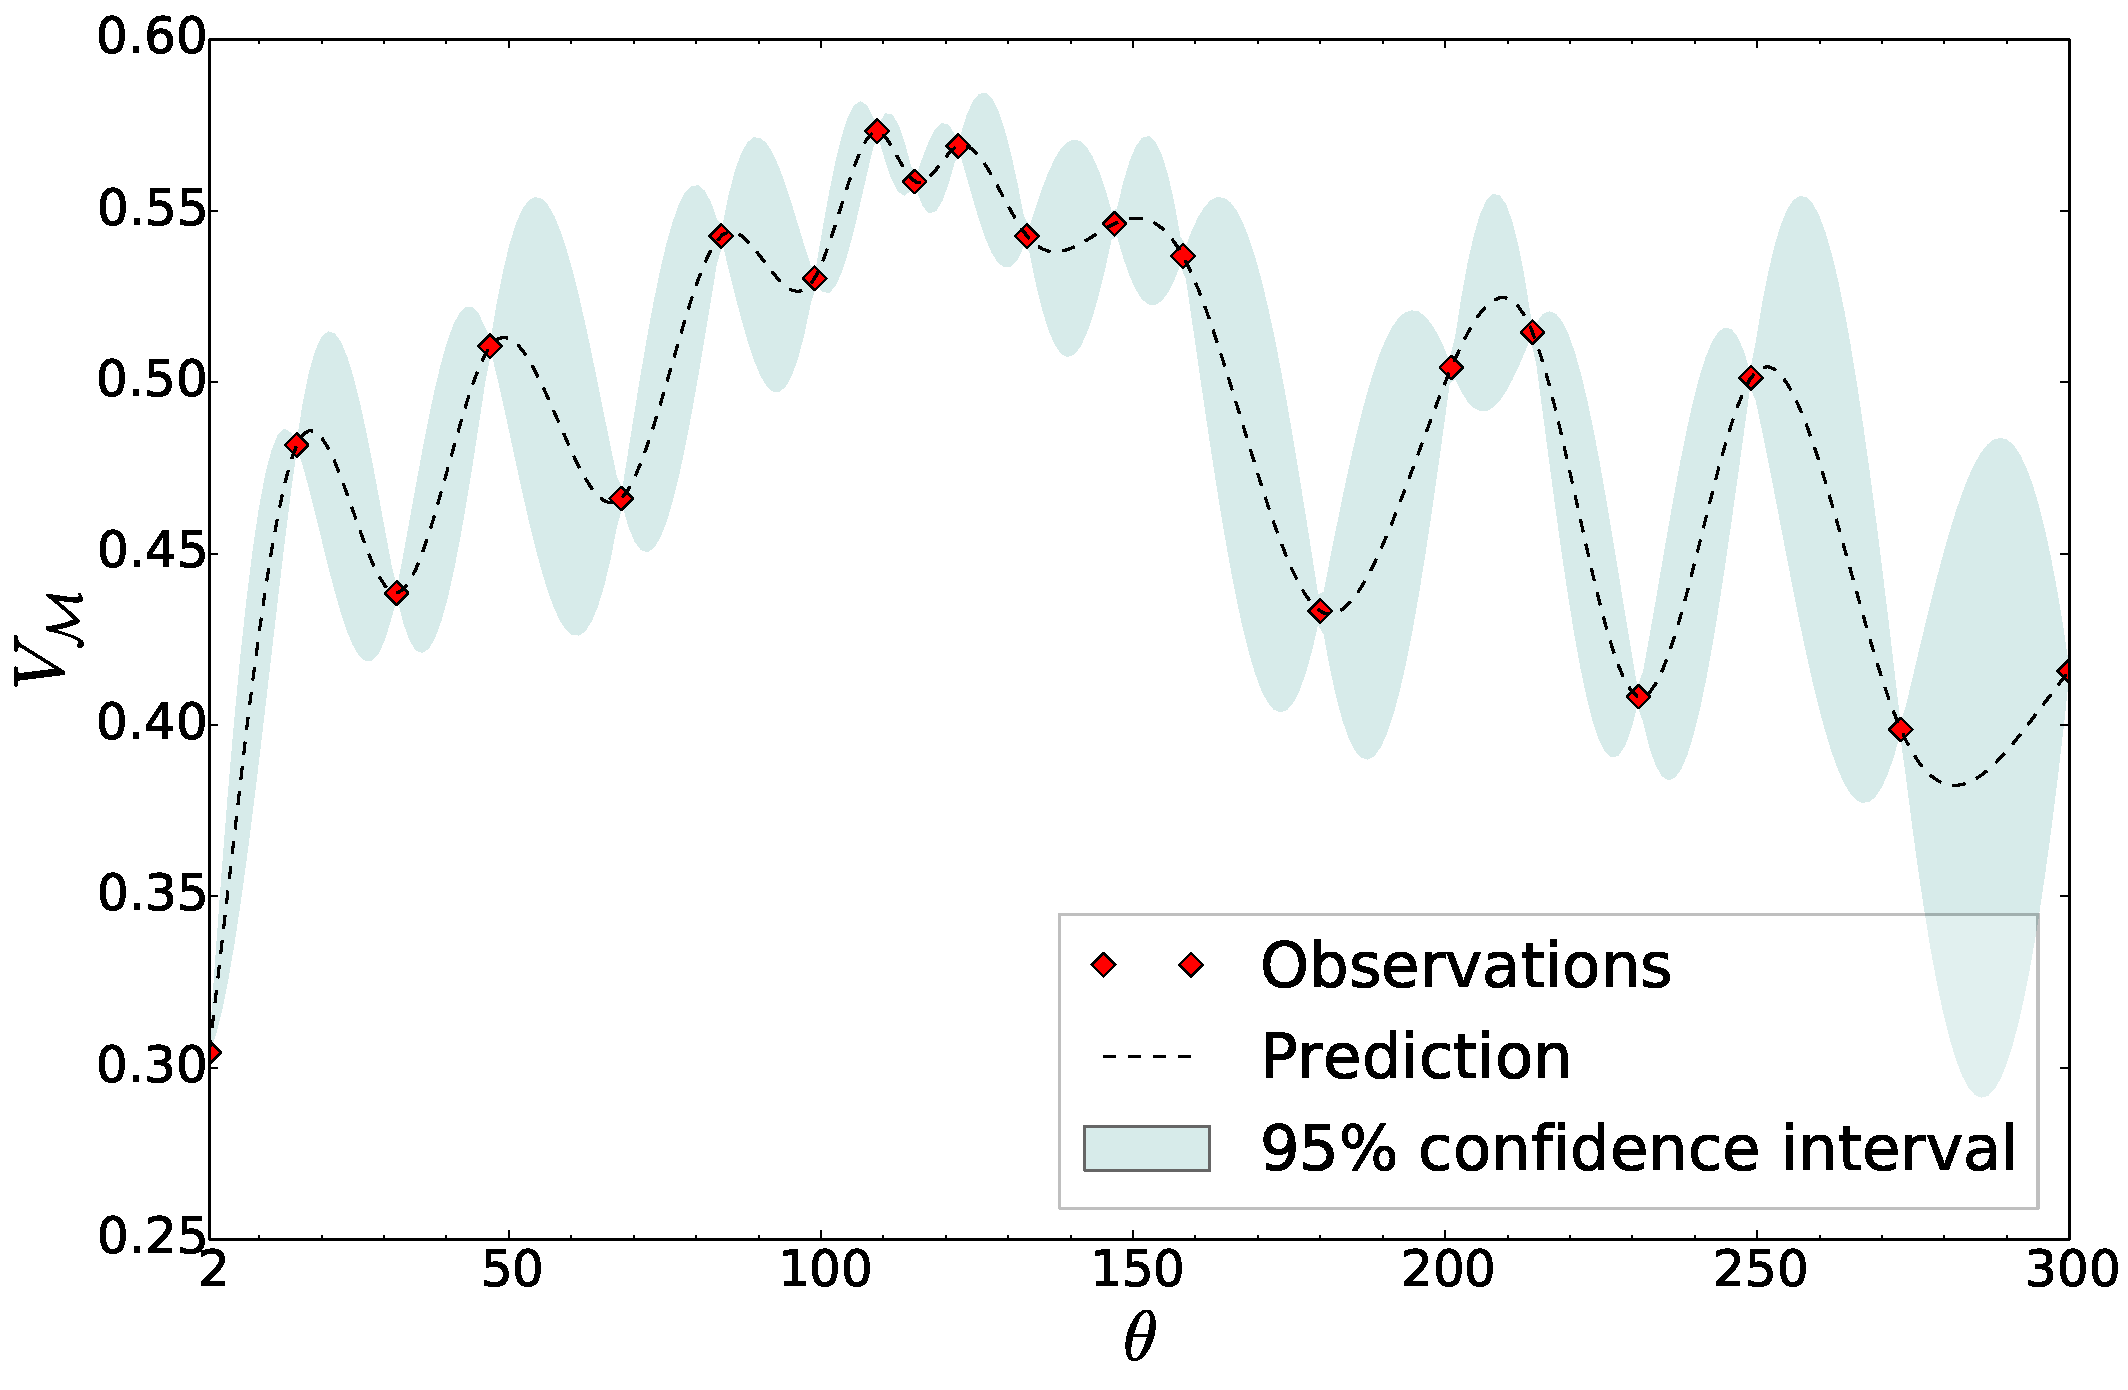
\includegraphics[width=\textwidth]{plots/tum_base/plot_b_00__alg_kmeans_pct_75_acq_ei}
		\caption{Experiment 2: 75\% of the dataset used}
		\label{fig:exp2}
	\end{subfigure}
	\begin{subfigure}[t]{0.495\textwidth}
		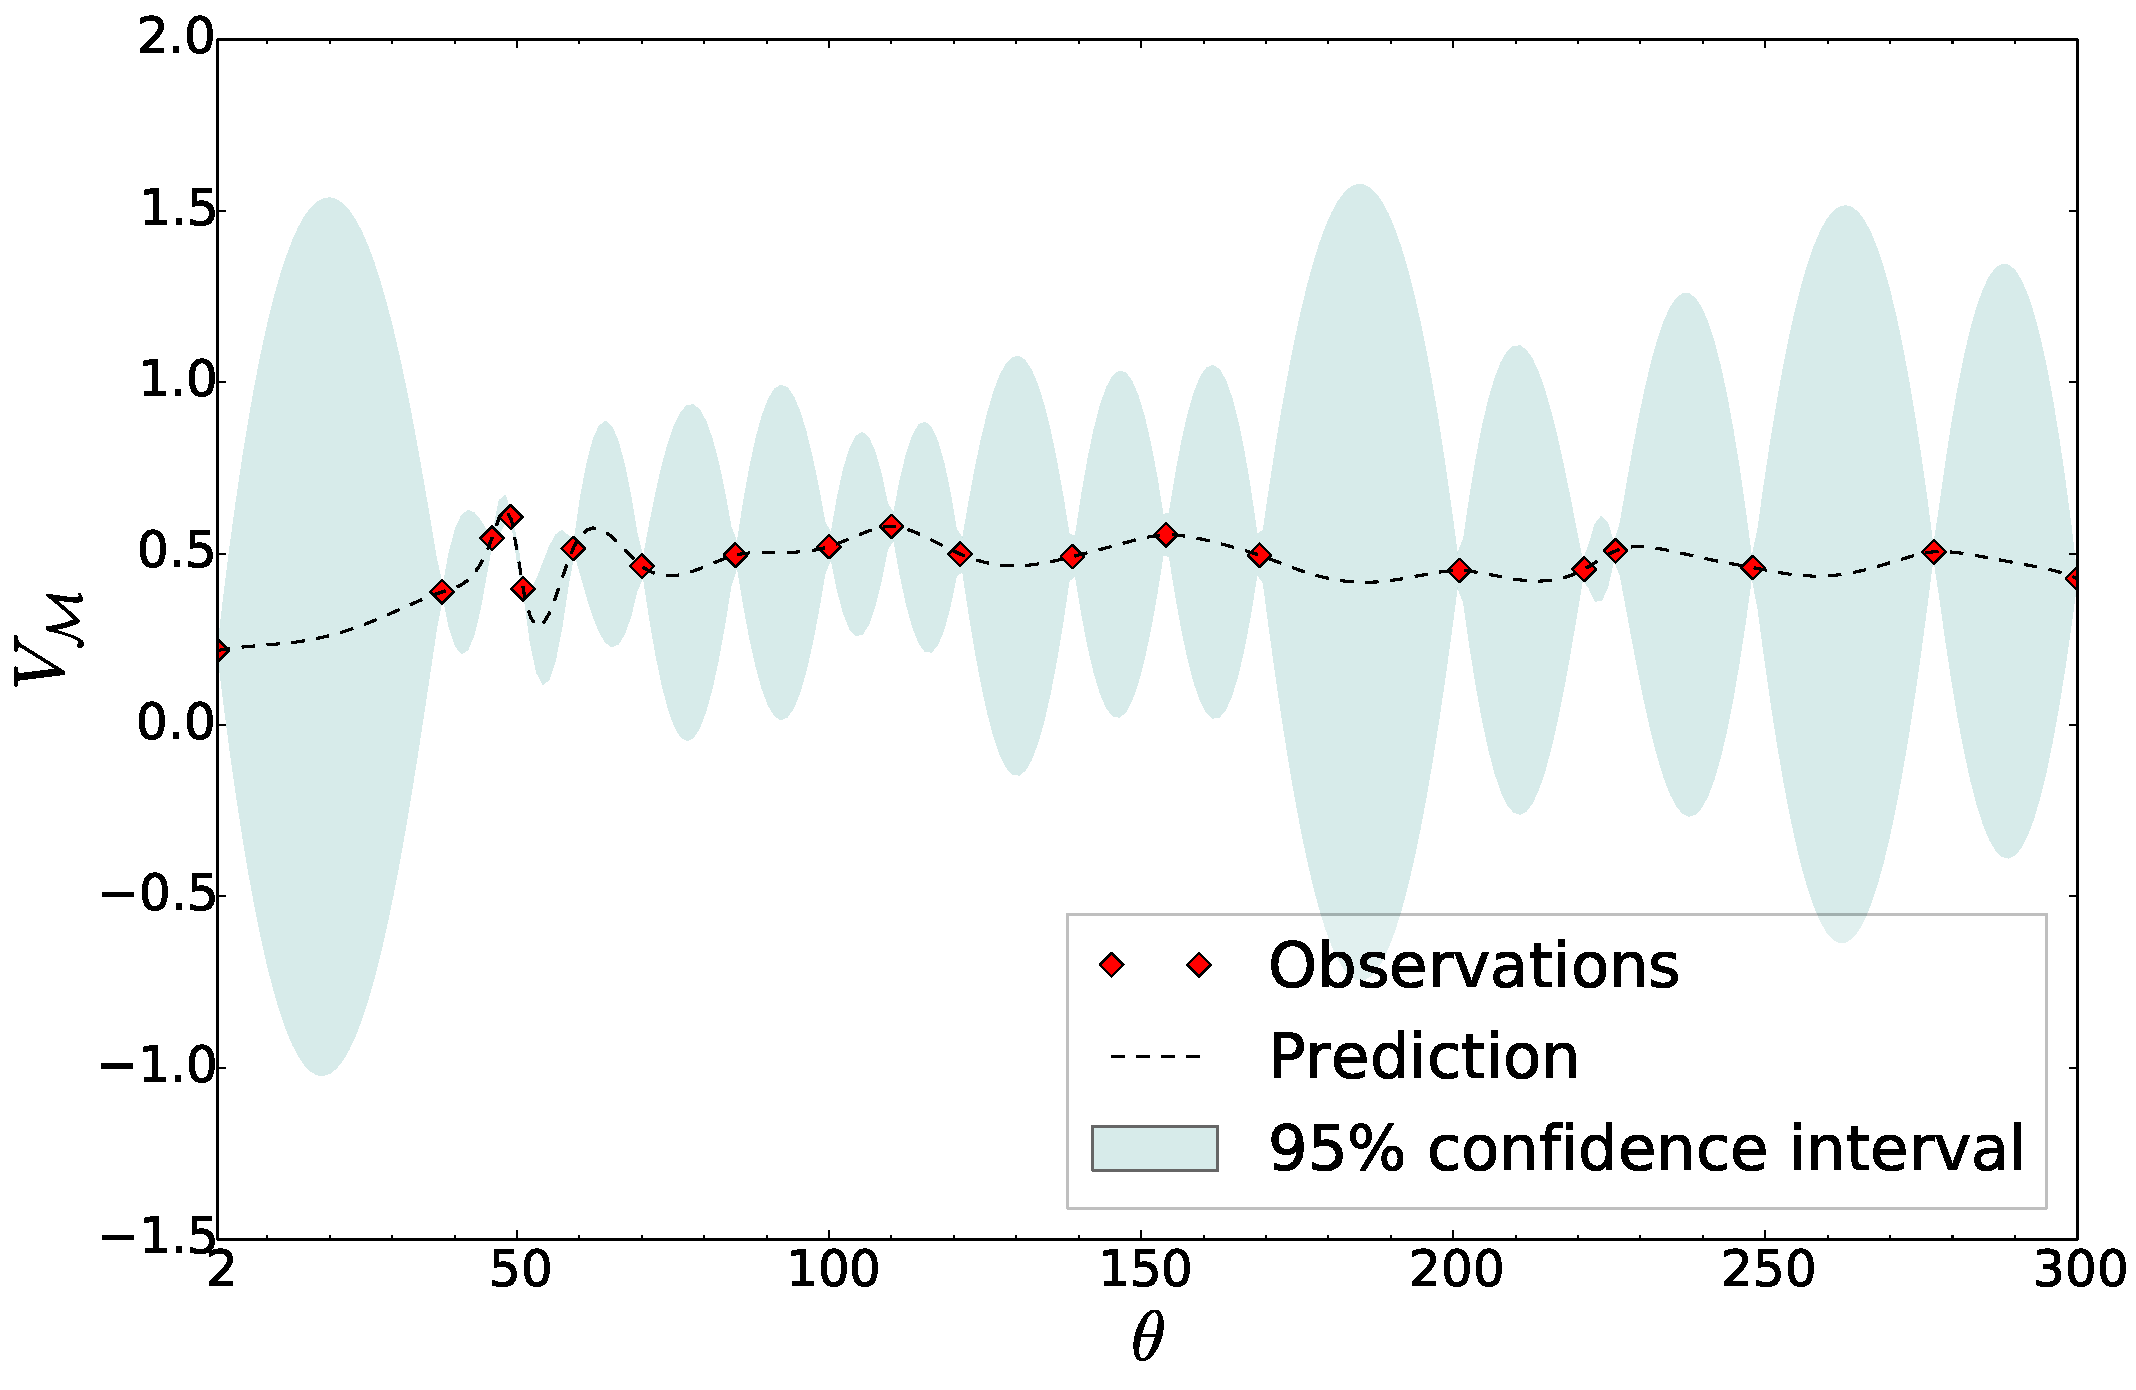
\includegraphics[width=\textwidth]{plots/tum_base/plot_b_00__alg_kmeans_pct_50_acq_ei}
		\caption{Experiment 3: 50\% of the dataset used}
		\label{fig:exp3}
	\end{subfigure}
	\caption{Plots showing a comparison of the resulting \acrshort{acr:gp} posterior for different dataset sizes. The plots correspond to 20 iterations of the base framework on the \texttt{tum\_kitchen} environment with $\beta = 0.0$, $k$-Means clustering and \acrshort{acr:mei} acquisition function used.}
	\label{fig:plots_tum_base_data}
\end{figure}

\subsubsection{Tum Kitchen Environment}

First of all, let us consider the results obtained for the small \texttt{tum\_kitchen} environment.
Overall, in \Crefrange{fig:plots_tum_base_acq}{fig:plots_tum_base_weight} one can see that the optimum $\theta_\mathsf{max}$ is mostly found within similar areas of the parameter space $\Theta$.
In \autoref{fig:plots_tum_base_data} we compare the effect of using different dataset sizes for learning \acrshortpl{acr:mdp}.
In \autoref{fig:exp1}, \autoref{fig:exp2} and \autoref{fig:exp3} the resulting \acrshort{acr:gp} is shown after respectively using 100\%, 75\% and 50\% of the dataset in the corresponding experiments.
One can see in \autoref{fig:exp3} that with 50\% of the data employed, the observed model values~$V_\mathcal{M}$ for different settings of $\theta$ involve quite some noise.
In this figure one can also see that the \acrshort{acr:gp} is quite sensitive to this noise and accordingly over-fits on these observations, so that the uncertainty about the parameter space is quite large.
At the other hand, \autoref{fig:exp2} shows that with 75\% of the data the distinction becomes much more clear, even though the higher variance is still present, particularly for larger settings of $\theta$.
This clearly shows that sufficient data is needed to avoid overfitting and obtaining more stable results with discernible performance measures.

%What might explain this, is that this particular section of the dataset adds data based on which \acrshortpl{acr:mdp} with large state spaces overfit their corresponding transition function.

\begin{figure}[t]
	\centering
	\captionsetup{font=small}
	\captionsetup[subfigure]{font=footnotesize}
	\captionsetup[subfigure]{justification=centering}
	\begin{subfigure}[t]{0.495\textwidth}
		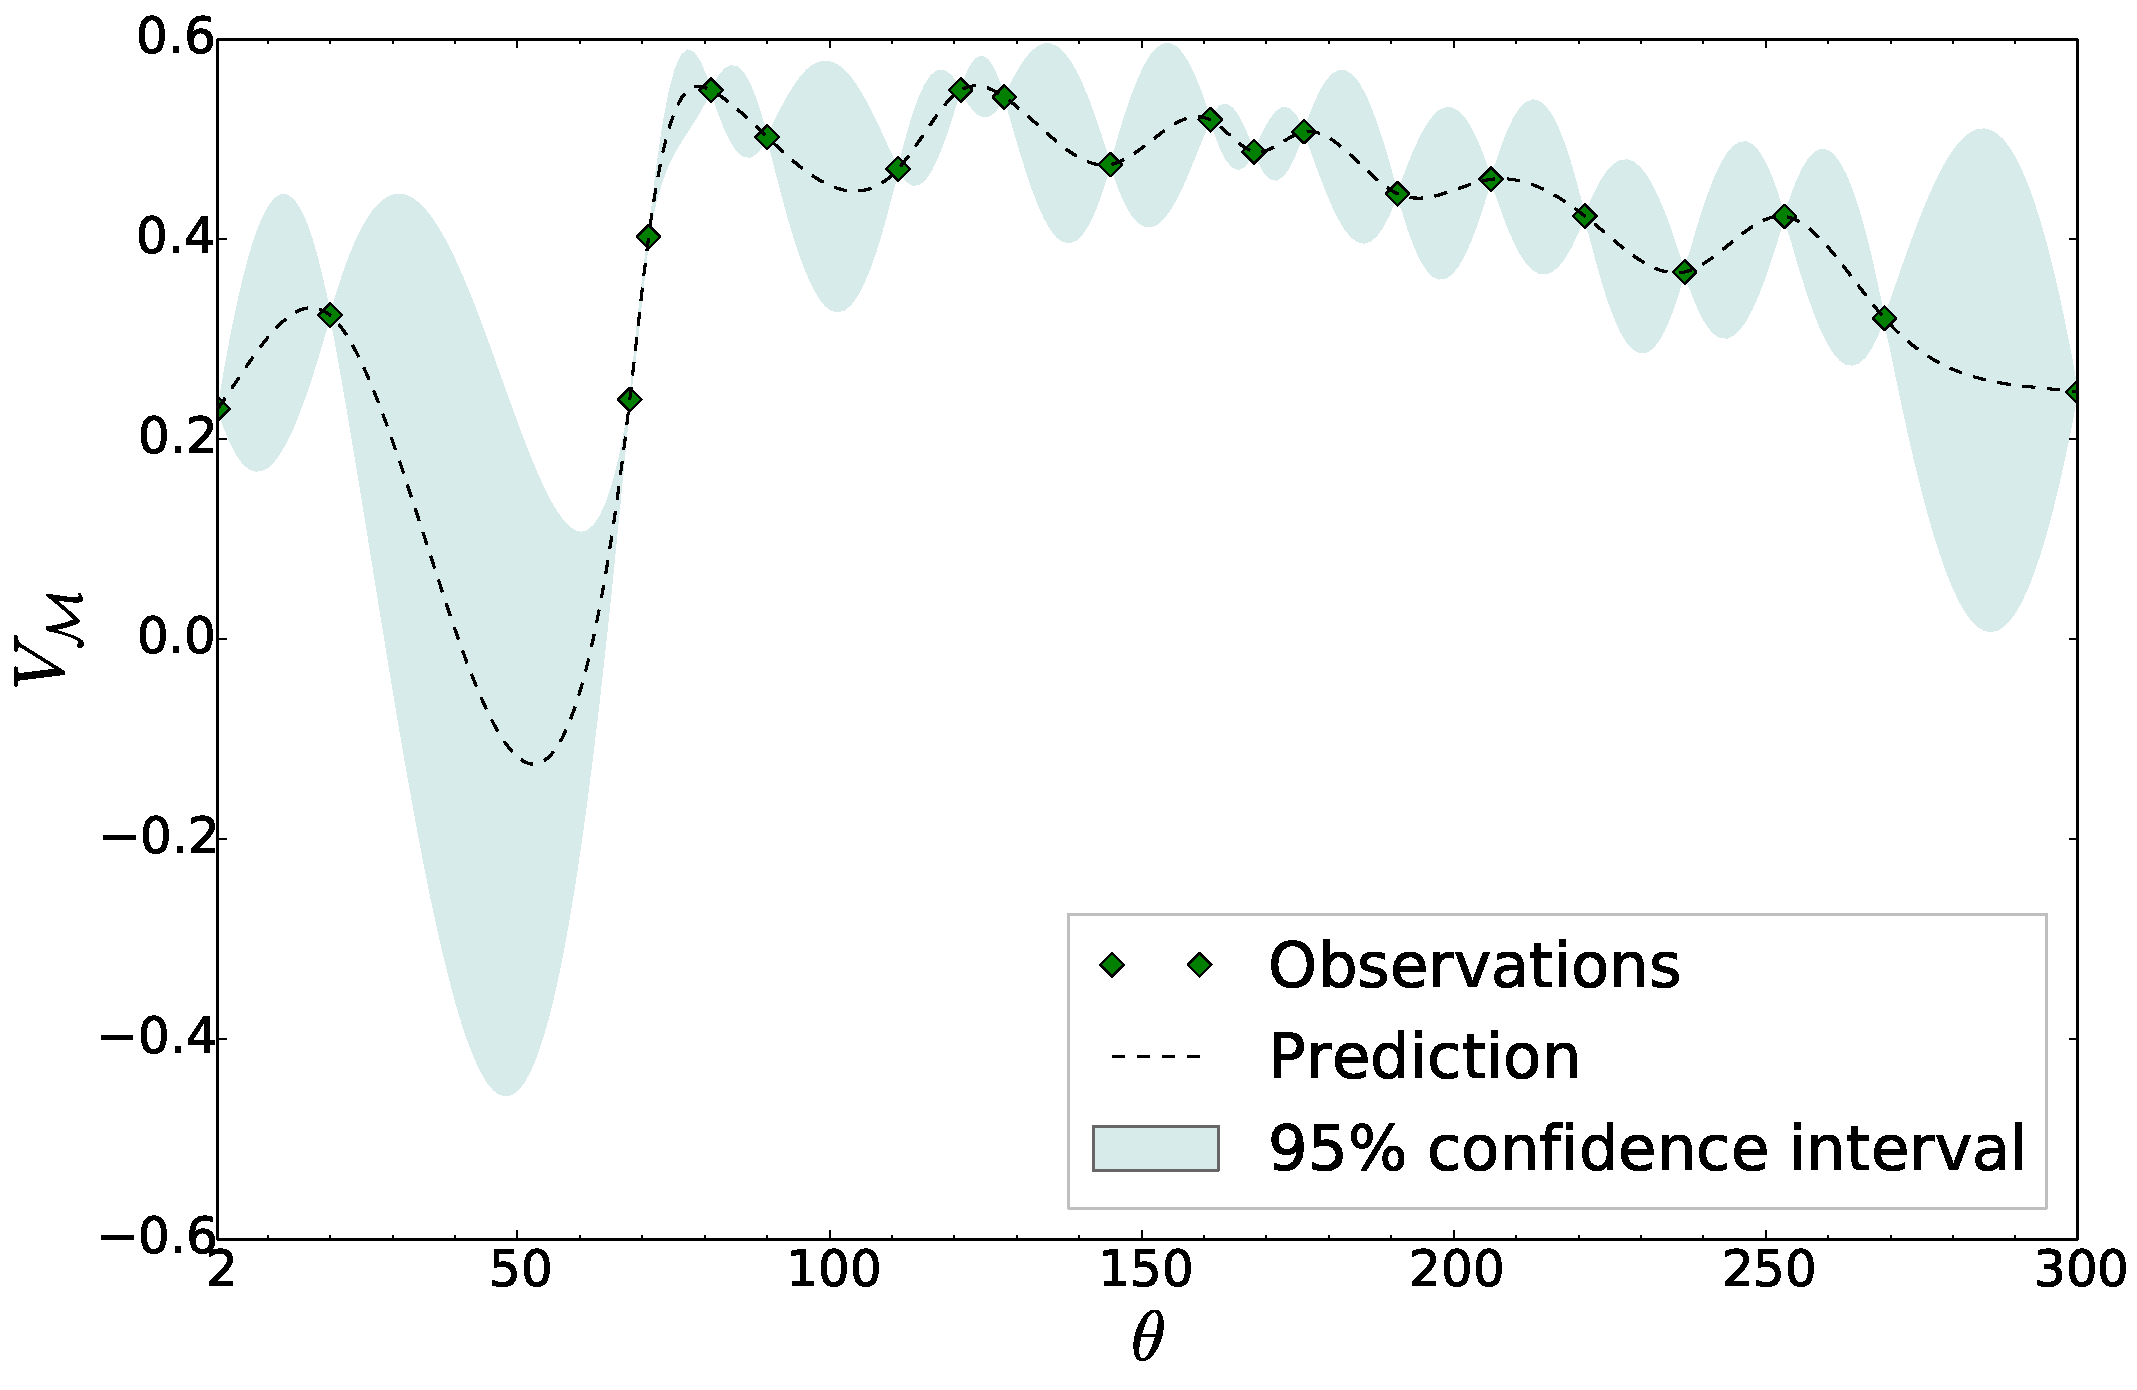
\includegraphics[width=\textwidth]{plots/tum_base/plot_b_00__alg_kmeans_pct_100_acq_ucb}
		\caption{Experiment 4: \acrshort{acr:gp-ucb} acquisition function used}
		\label{fig:exp4}
	\end{subfigure}
	\begin{subfigure}[t]{0.495\textwidth}
		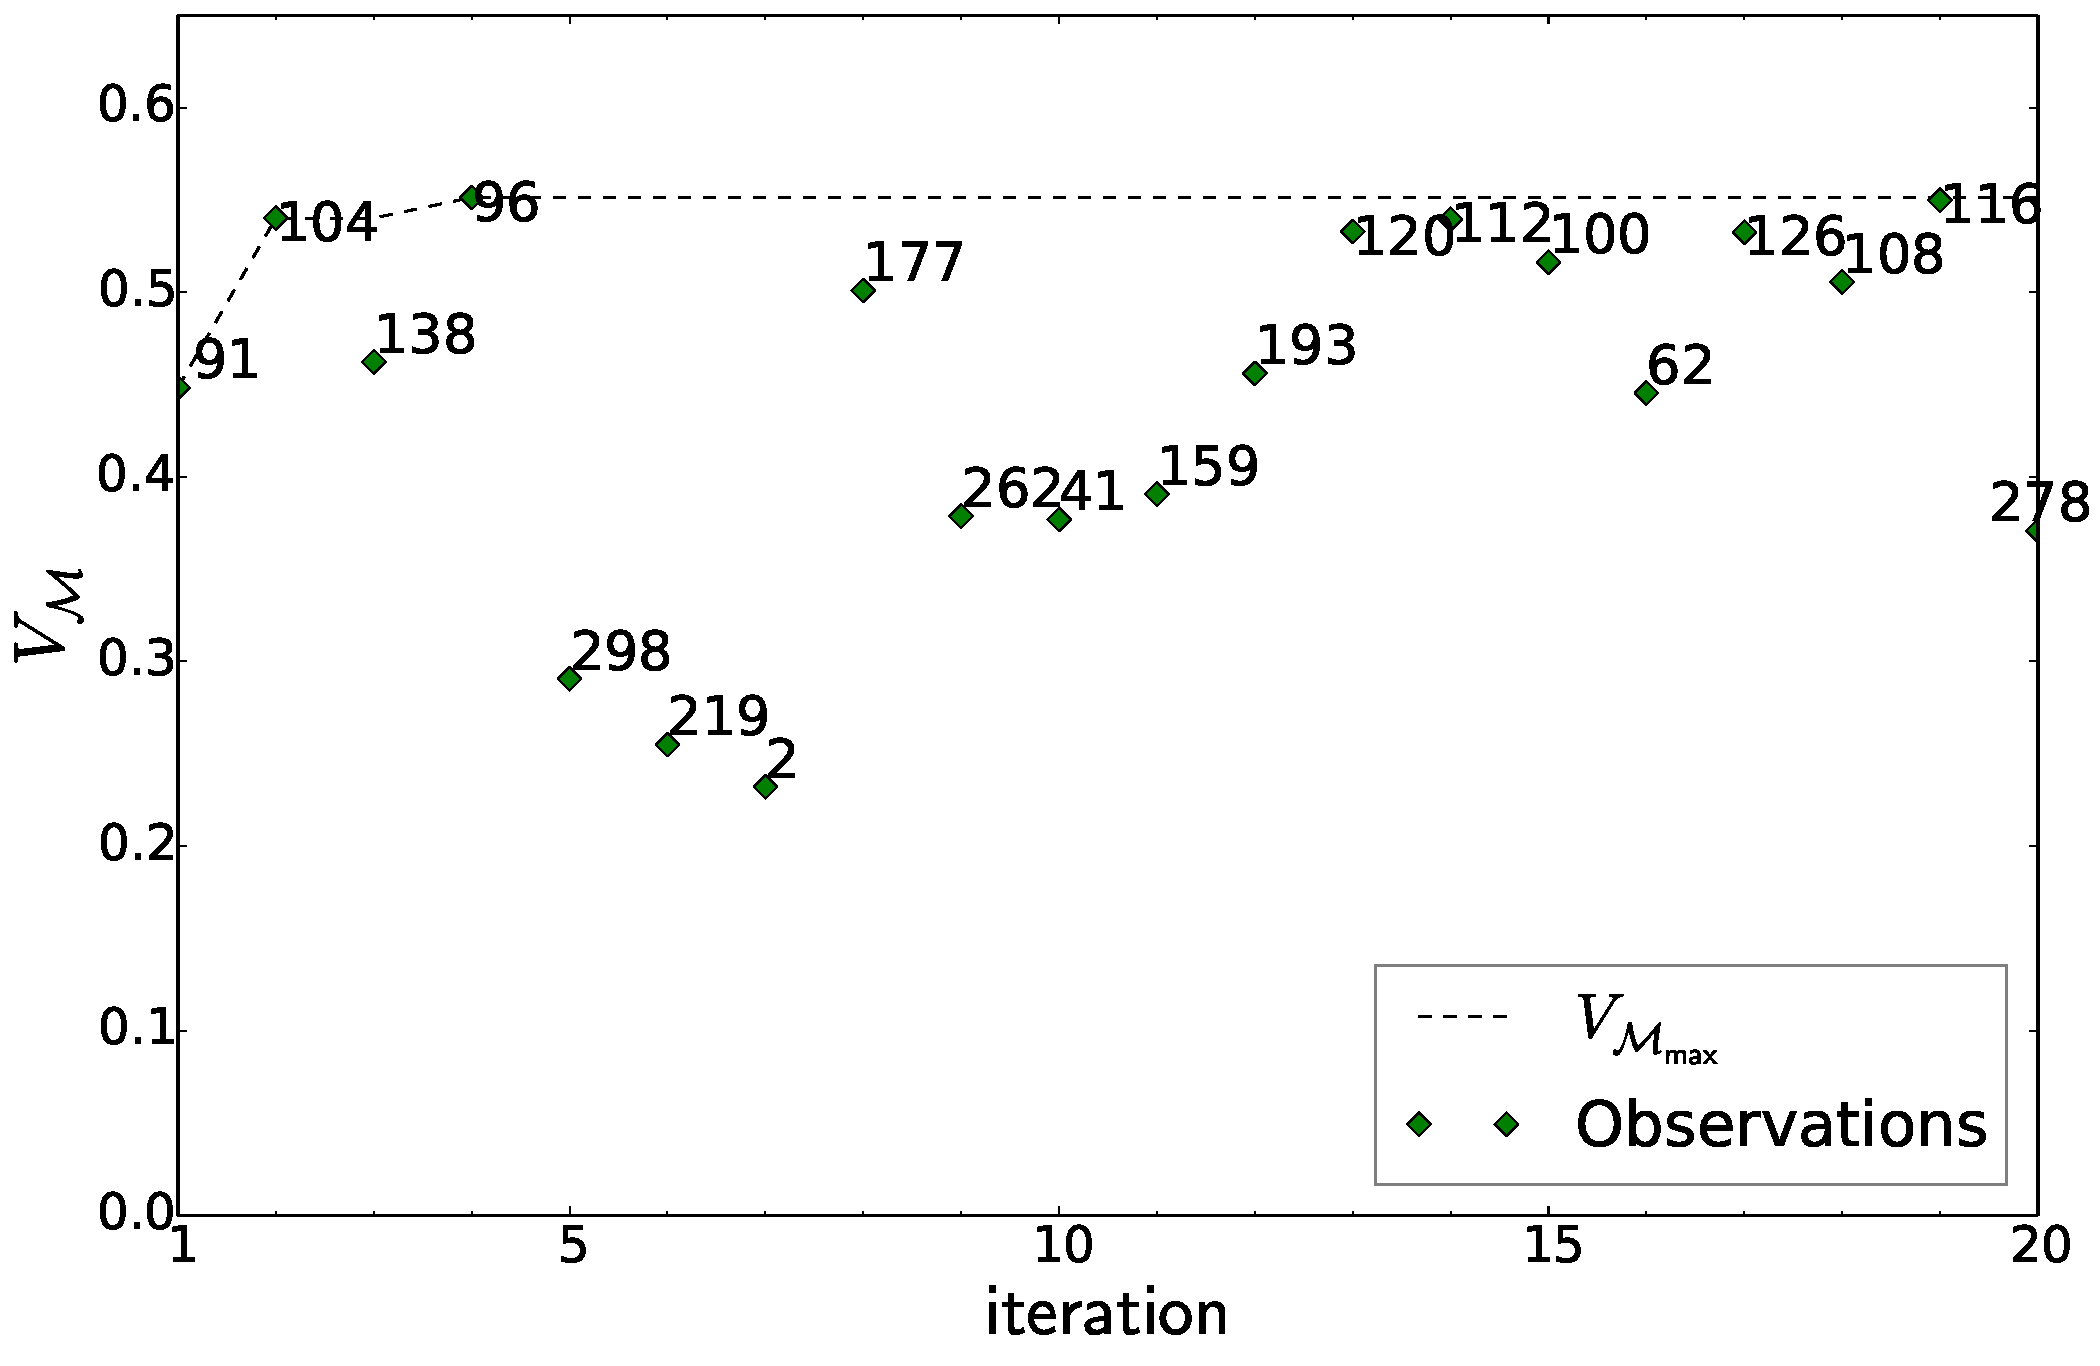
\includegraphics[width=\textwidth]{plots/tum_base/plot_b_00__alg_kmeans_pct_100_acq_ucb_maximum_2}
		\caption{Experiment 4: Observations over iterations}
		\label{fig:exp4_observations}
	\end{subfigure}
	\begin{subfigure}[t]{0.495\textwidth}
		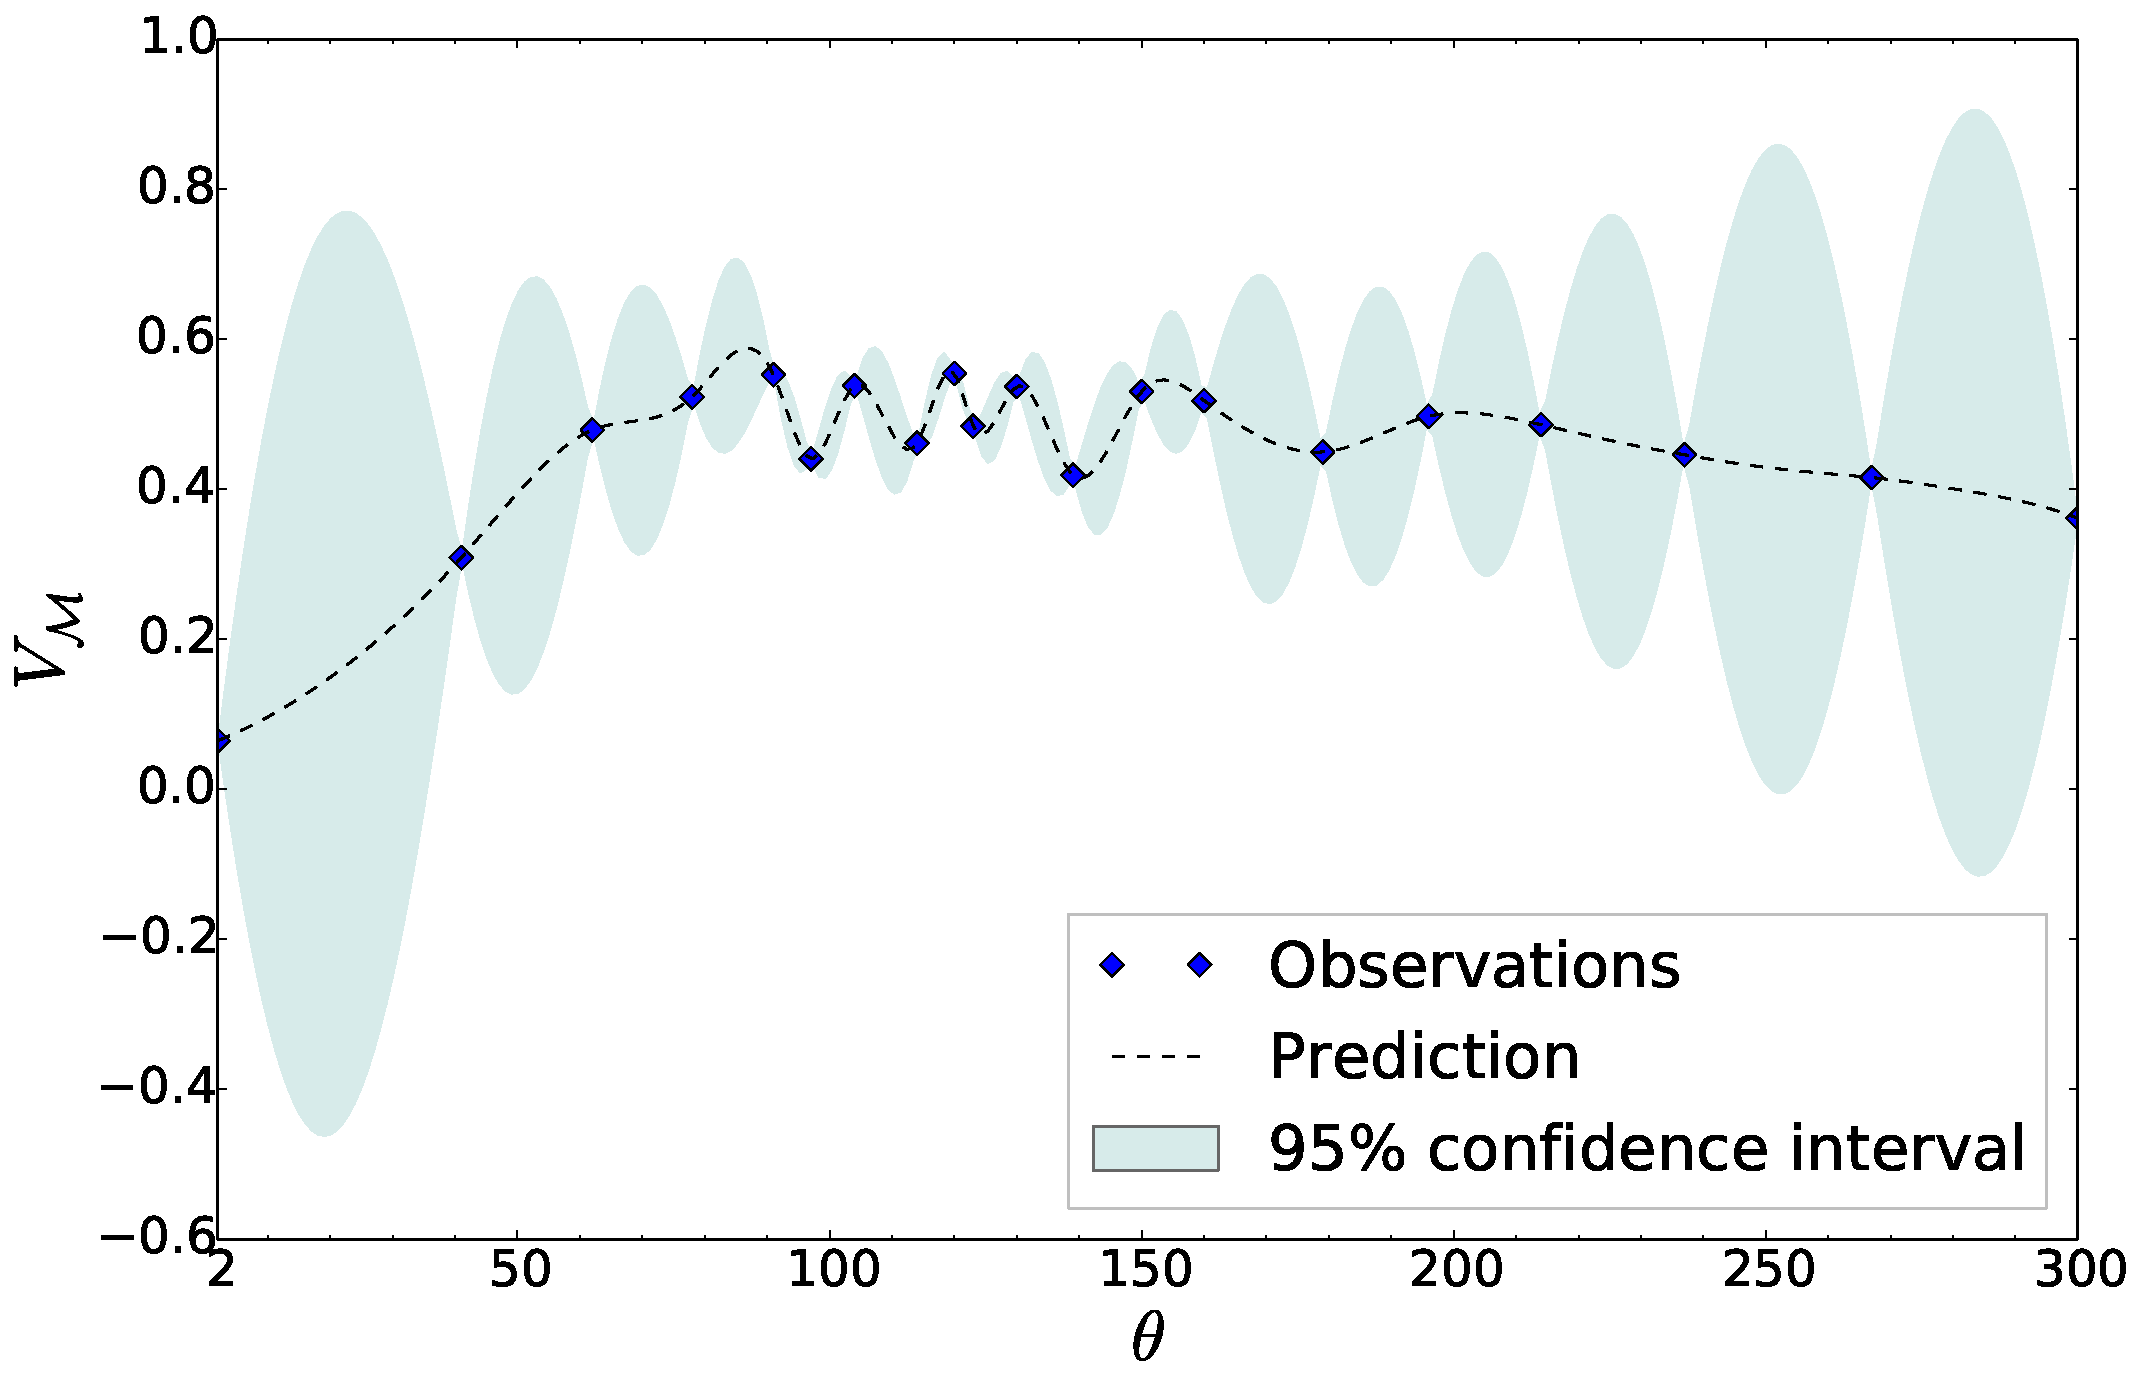
\includegraphics[width=\textwidth]{plots/tum_base/plot_b_00__alg_kmeans_pct_100_acq_eips}
		\caption{Experiment 5: \acrshort{acr:mei-ps} acquisition function used}
		\label{fig:exp5}
	\end{subfigure}
	\begin{subfigure}[t]{0.495\textwidth}
		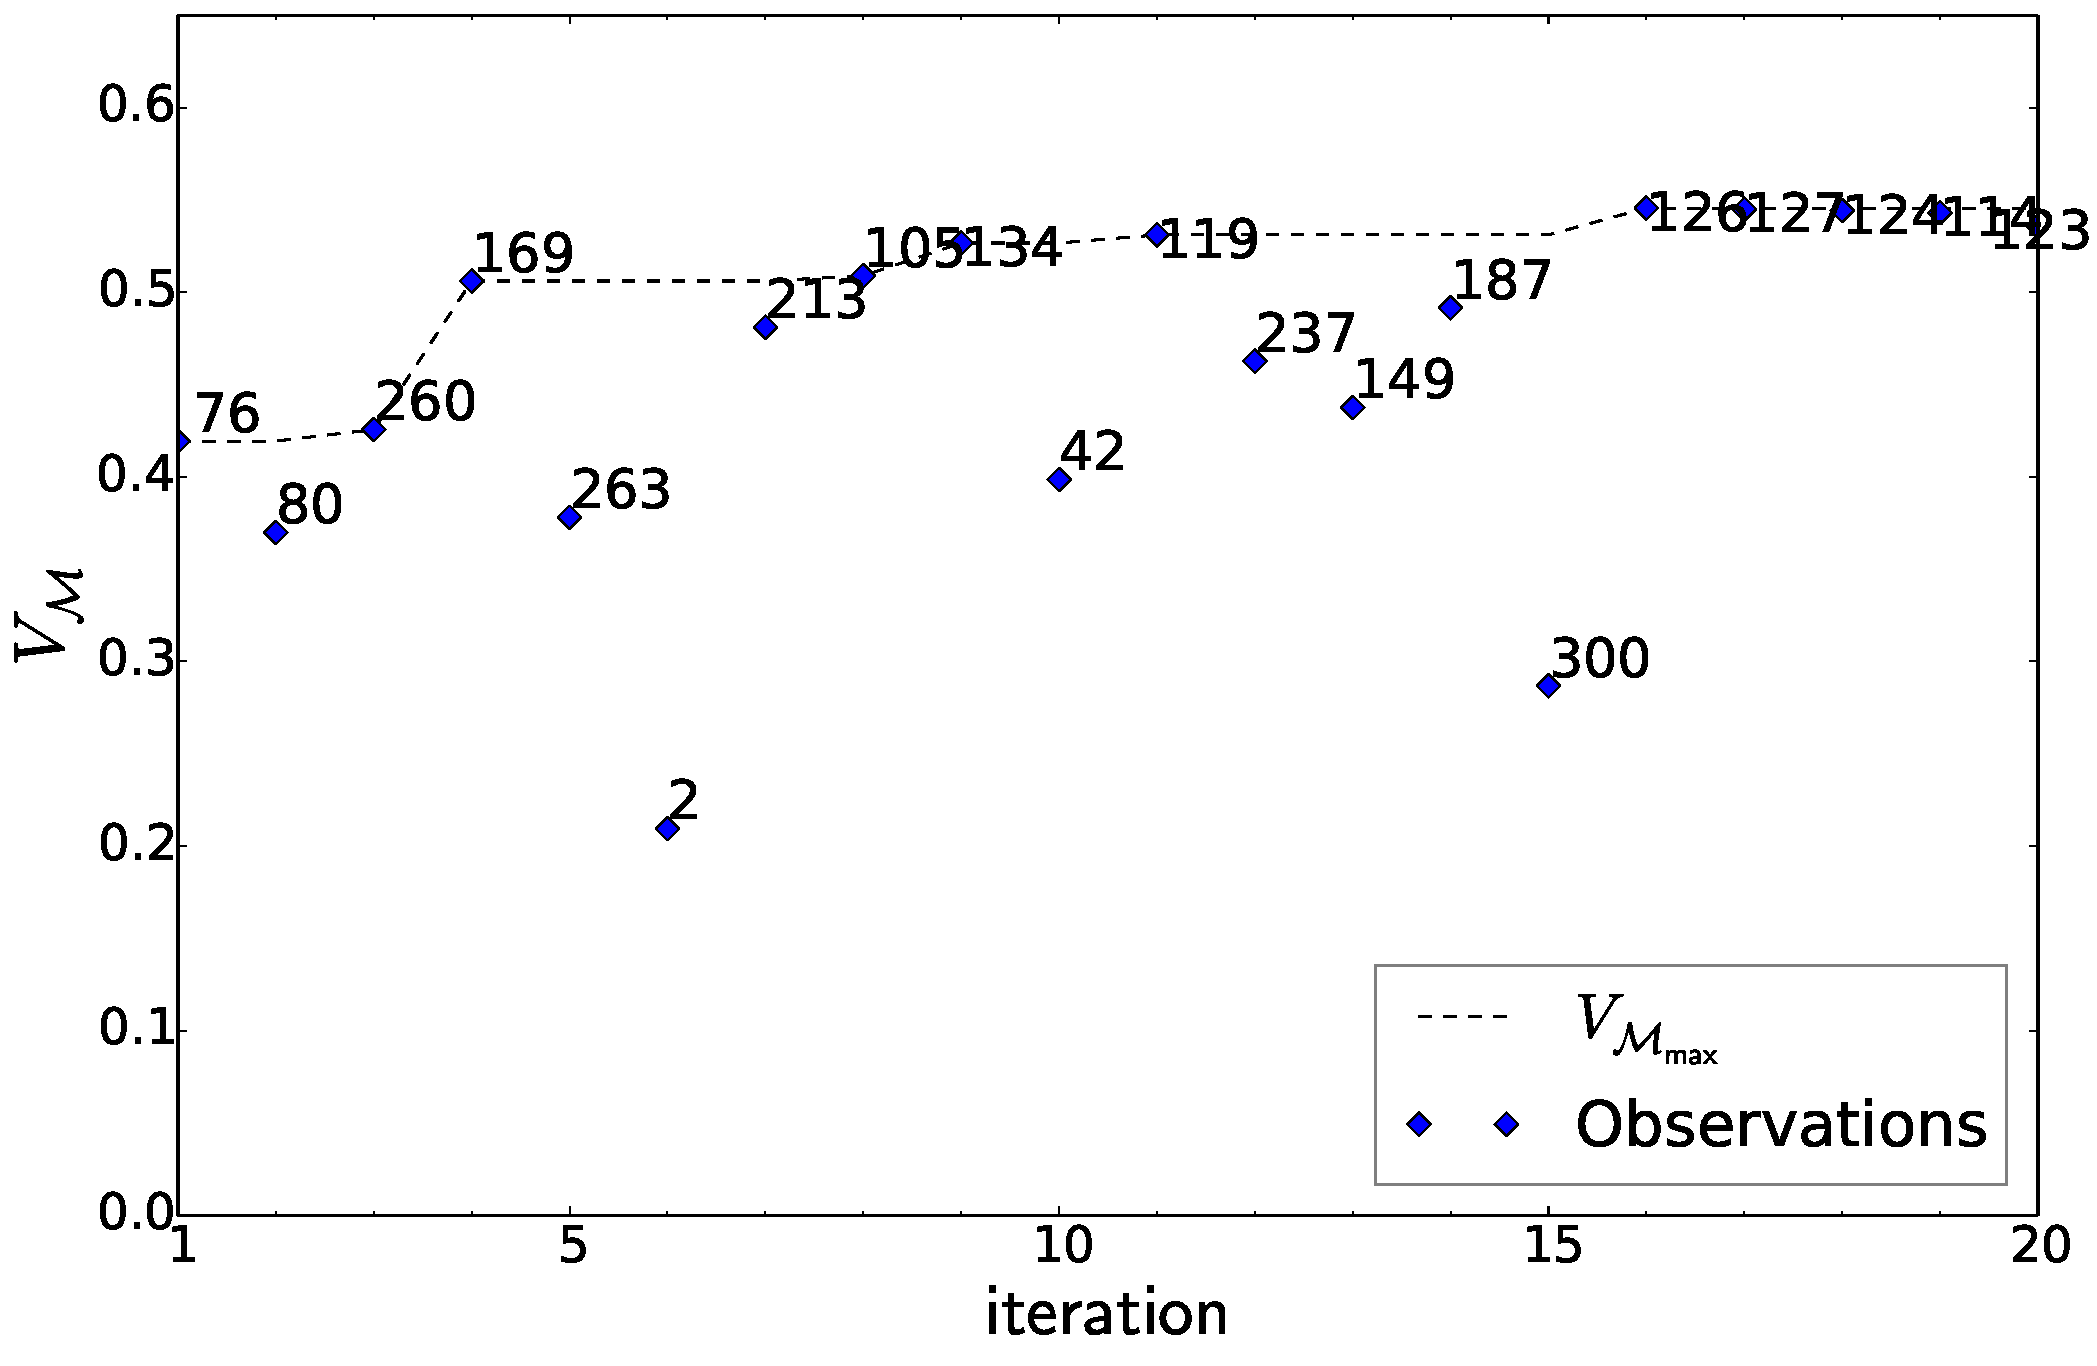
\includegraphics[width=\textwidth]{plots/tum_base/plot_b_00__alg_kmeans_pct_100_acq_eips_maximum_2}
		\caption{Experiment 5: Observations over iterations}
		\label{fig:exp5_observations}
	\end{subfigure}
	\caption{Plots showing a comparison of the resulting \acrshort{acr:gp} posterior for varying acquisition functions. The plots correspond to 20 iterations of the base framework on the \texttt{tum\_kitchen} environment with $\beta = 0.0$ and $k$-Means~clustering used.}
	\label{fig:plots_tum_base_acq}
\end{figure}

\begin{figure}[t!]
	\centering
	\captionsetup{font=small}
	\captionsetup[subfigure]{font=footnotesize}
	\captionsetup[subfigure]{justification=centering}
	\begin{subfigure}[t]{0.495\textwidth}
		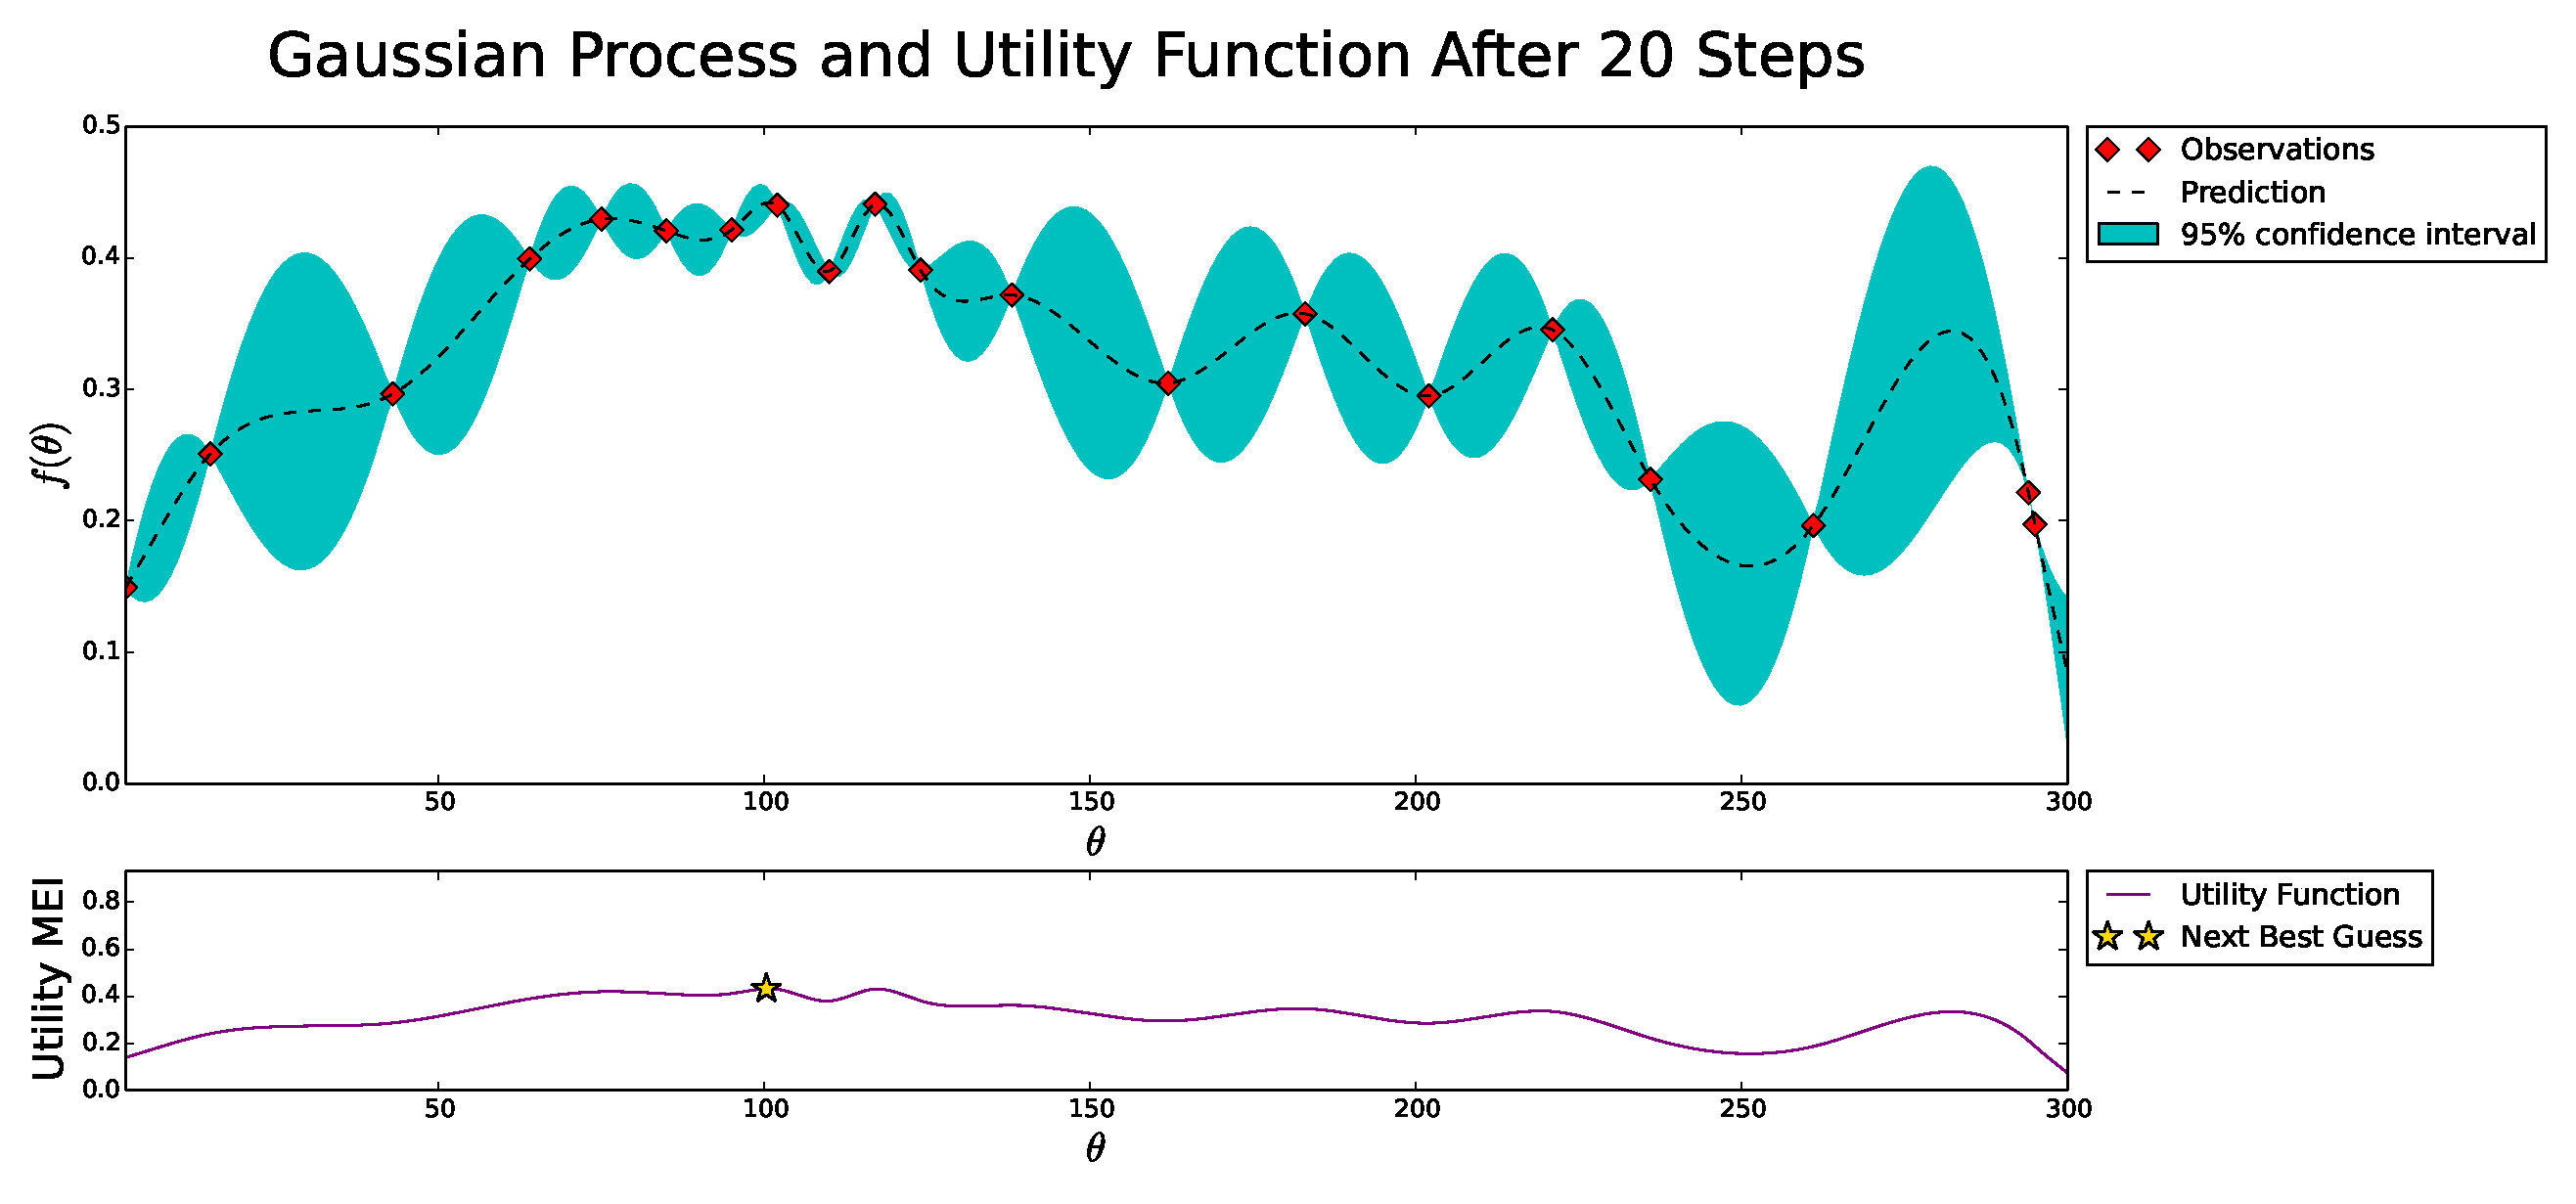
\includegraphics[width=\textwidth]{plots/tum_base/plot_b_00__alg_gmm_pct_100_acq_ei}
		\caption{Experiment 6: \acrshort{acr:mei} acquisition function used}
		\label{fig:exp6}
	\end{subfigure}
	\begin{subfigure}[t]{0.495\textwidth}
		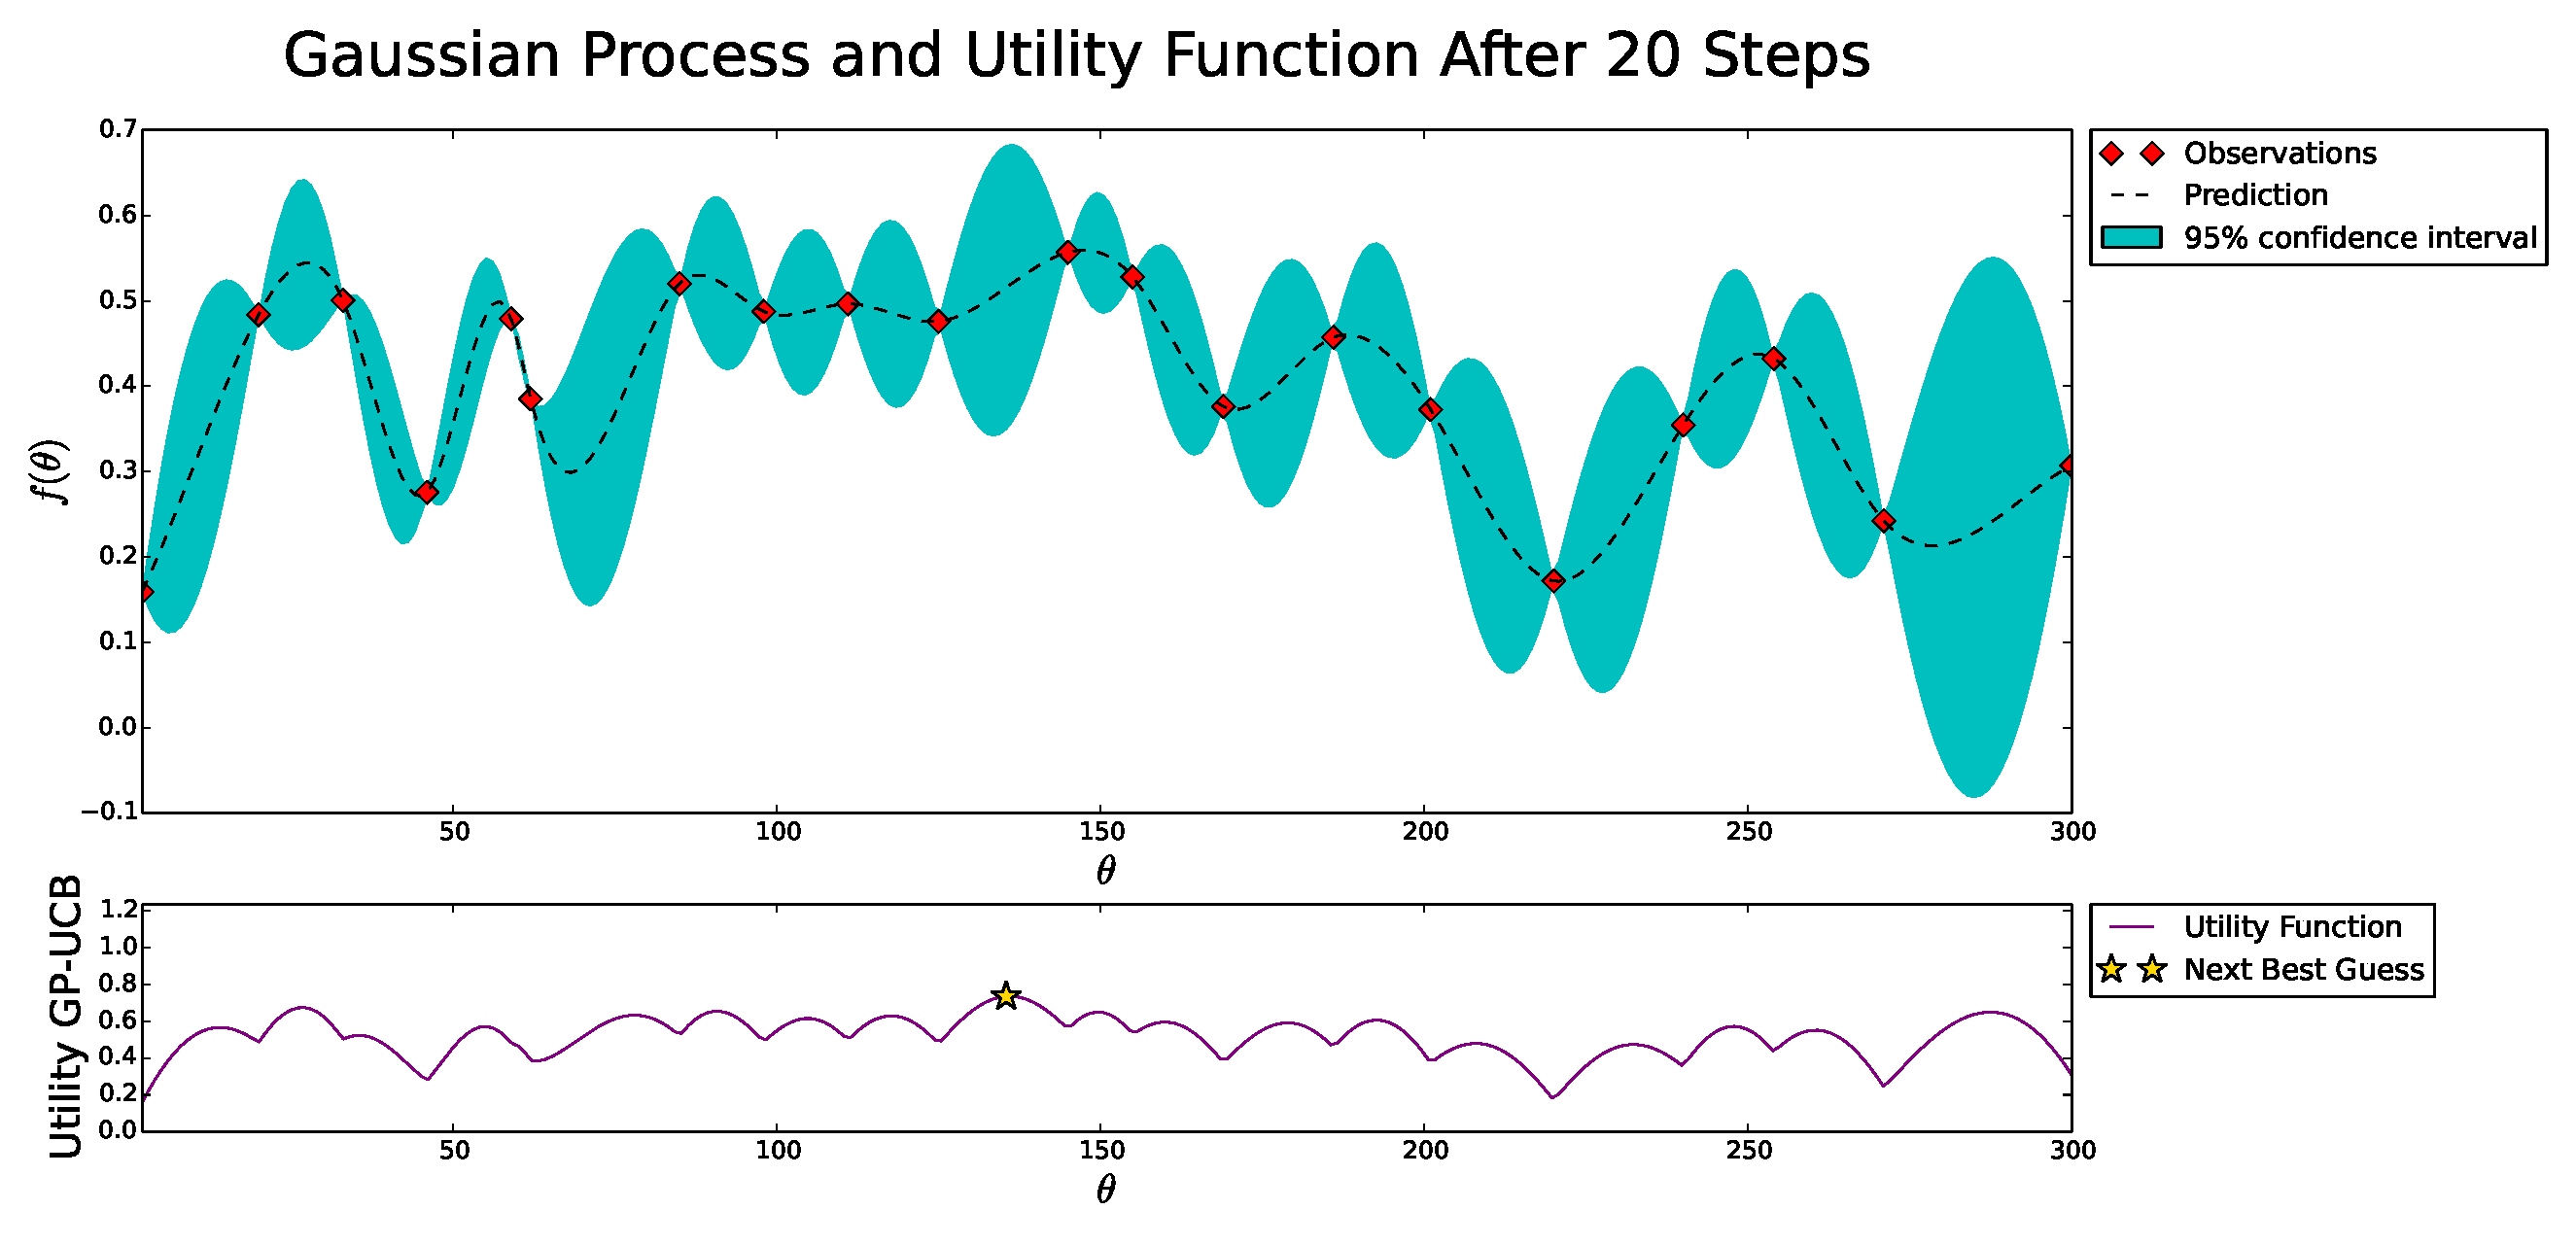
\includegraphics[width=\textwidth]{plots/tum_base/plot_b_00__alg_gmm_pct_100_acq_ucb}
		\caption{Experiment 7: \acrshort{acr:gp-ucb} acquisition function used}
		\label{fig:exp7}
	\end{subfigure}
	\caption{Plots showing a comparison of the resulting \acrshort{acr:gp} posterior for varying acquisition functions. The plots correspond to 20 iterations of the base framework on the \texttt{tum\_kitchen} environment with $\beta = 0.0$ and \acrshort{acr:gmm}~used.}
	\label{fig:plots_tum_base_gmm}
\end{figure}

\newpage

Next, let us compare the results depicted in \autoref{fig:exp1} and \autoref{fig:plots_tum_base_acq} where different acquisition functions are used in the \acrshort{acr:bo} framework (i.e., \acrshort{acr:mei}, \acrshort{acr:gp-ucb} and \acrshort{acr:mei-ps} respectively).
In addition, we present some plots that show how the different acquisition function samples new observations in \autoref{fig:exp1_observations}, \autoref{fig:exp4_observations} and \autoref{fig:exp5_observations}.

First of all, we see that in each of these experiments a global maximum is found in the same area of the parameter space.
%For this environment, we see the results are quite similar, and also in the logs made from the experiments it was seen that the maximum observation was done in the (exact) same number of steps (in the third step).
%The most clear difference is seen in the `behavior' of the \acrshort{acr:gp-ucb} acquisition function, being optimistic in the face of uncertainty, so that the confidence intervals are restricted for promising areas of the parameter space.
%On the other hand, the influence of the timing \acrshort{acr:gp} in the \acrshort{acr:mei-ps} acquisition  is absent for our experiments in the \texttt{tum\_kitchen} environment, as the difference in the required time for model learning and planning is minimal.
For this environment the \acrshort{acr:gp-ucb} and \acrshort{acr:mei-ps} lead to a more clear convergence to the area of the parameter space with the global optimum.
The benefits of the timing \acrshort{acr:gp} in the \acrshort{acr:mei-ps} is only limited for this environment as the time for model learning and planning are closer together than for the \texttt{uol\_bl} environment.

Then, in \autoref{fig:exp6} and \autoref{fig:exp7} we see the plots for the experiments in which instead \acrshortpl{acr:gmm} are used for learning state spaces for our \acrshortpl{acr:mdp}.
We observe that again for this algorithm, the optima are found within the same areas of the parameter space for both experiments with different acquisition functions.
The main thing we observe is that, the observed model values $V_\mathcal{M}$ is overall lower with the \acrshort{acr:gmm} employed in comparison to the values observed with $k$-Means employed.
Therefore, employing $k$-Means appears more suitable to learn the state space for \acrshortpl{acr:mdp} in our application of mobile robot navigation.

\begin{figure}[!t]
	\centering
	\captionsetup{font=small}
	\captionsetup[subfigure]{font=footnotesize}
	\captionsetup[subfigure]{justification=centering}
	\begin{subfigure}[t]{0.495\textwidth}
		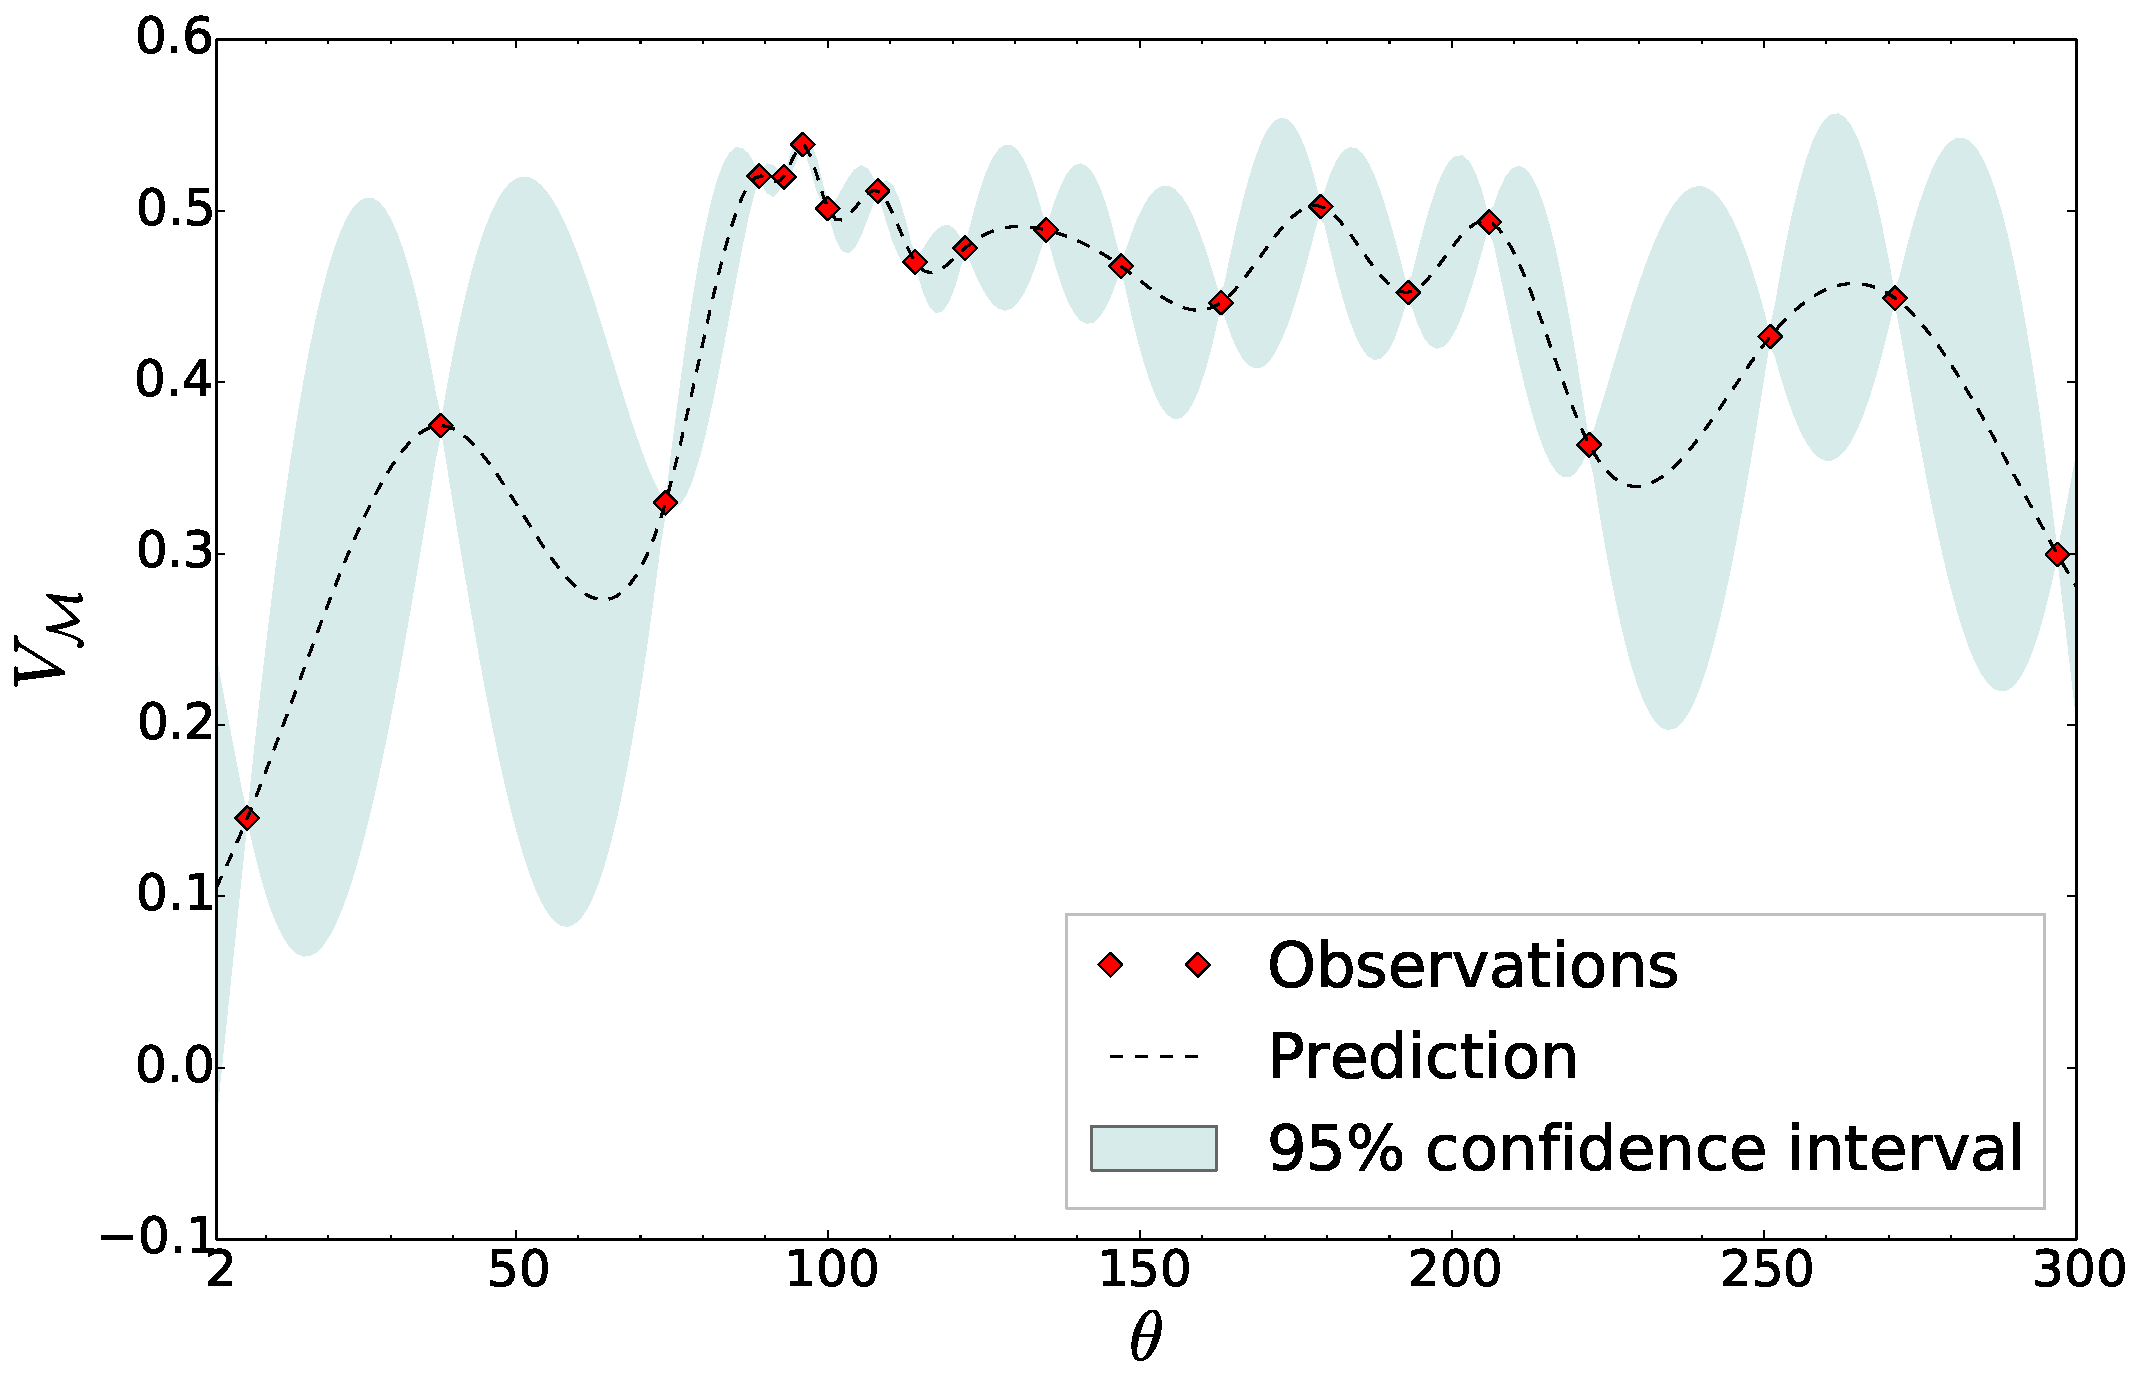
\includegraphics[width=\textwidth]{plots/tum_base/plot_b_025__alg_kmeans_pct_100_acq_ei}
		\caption{Experiment 8: Weight factor $\beta = 0.25$}
		\label{fig:exp8}
	\end{subfigure}
	\begin{subfigure}[t]{0.495\textwidth}
		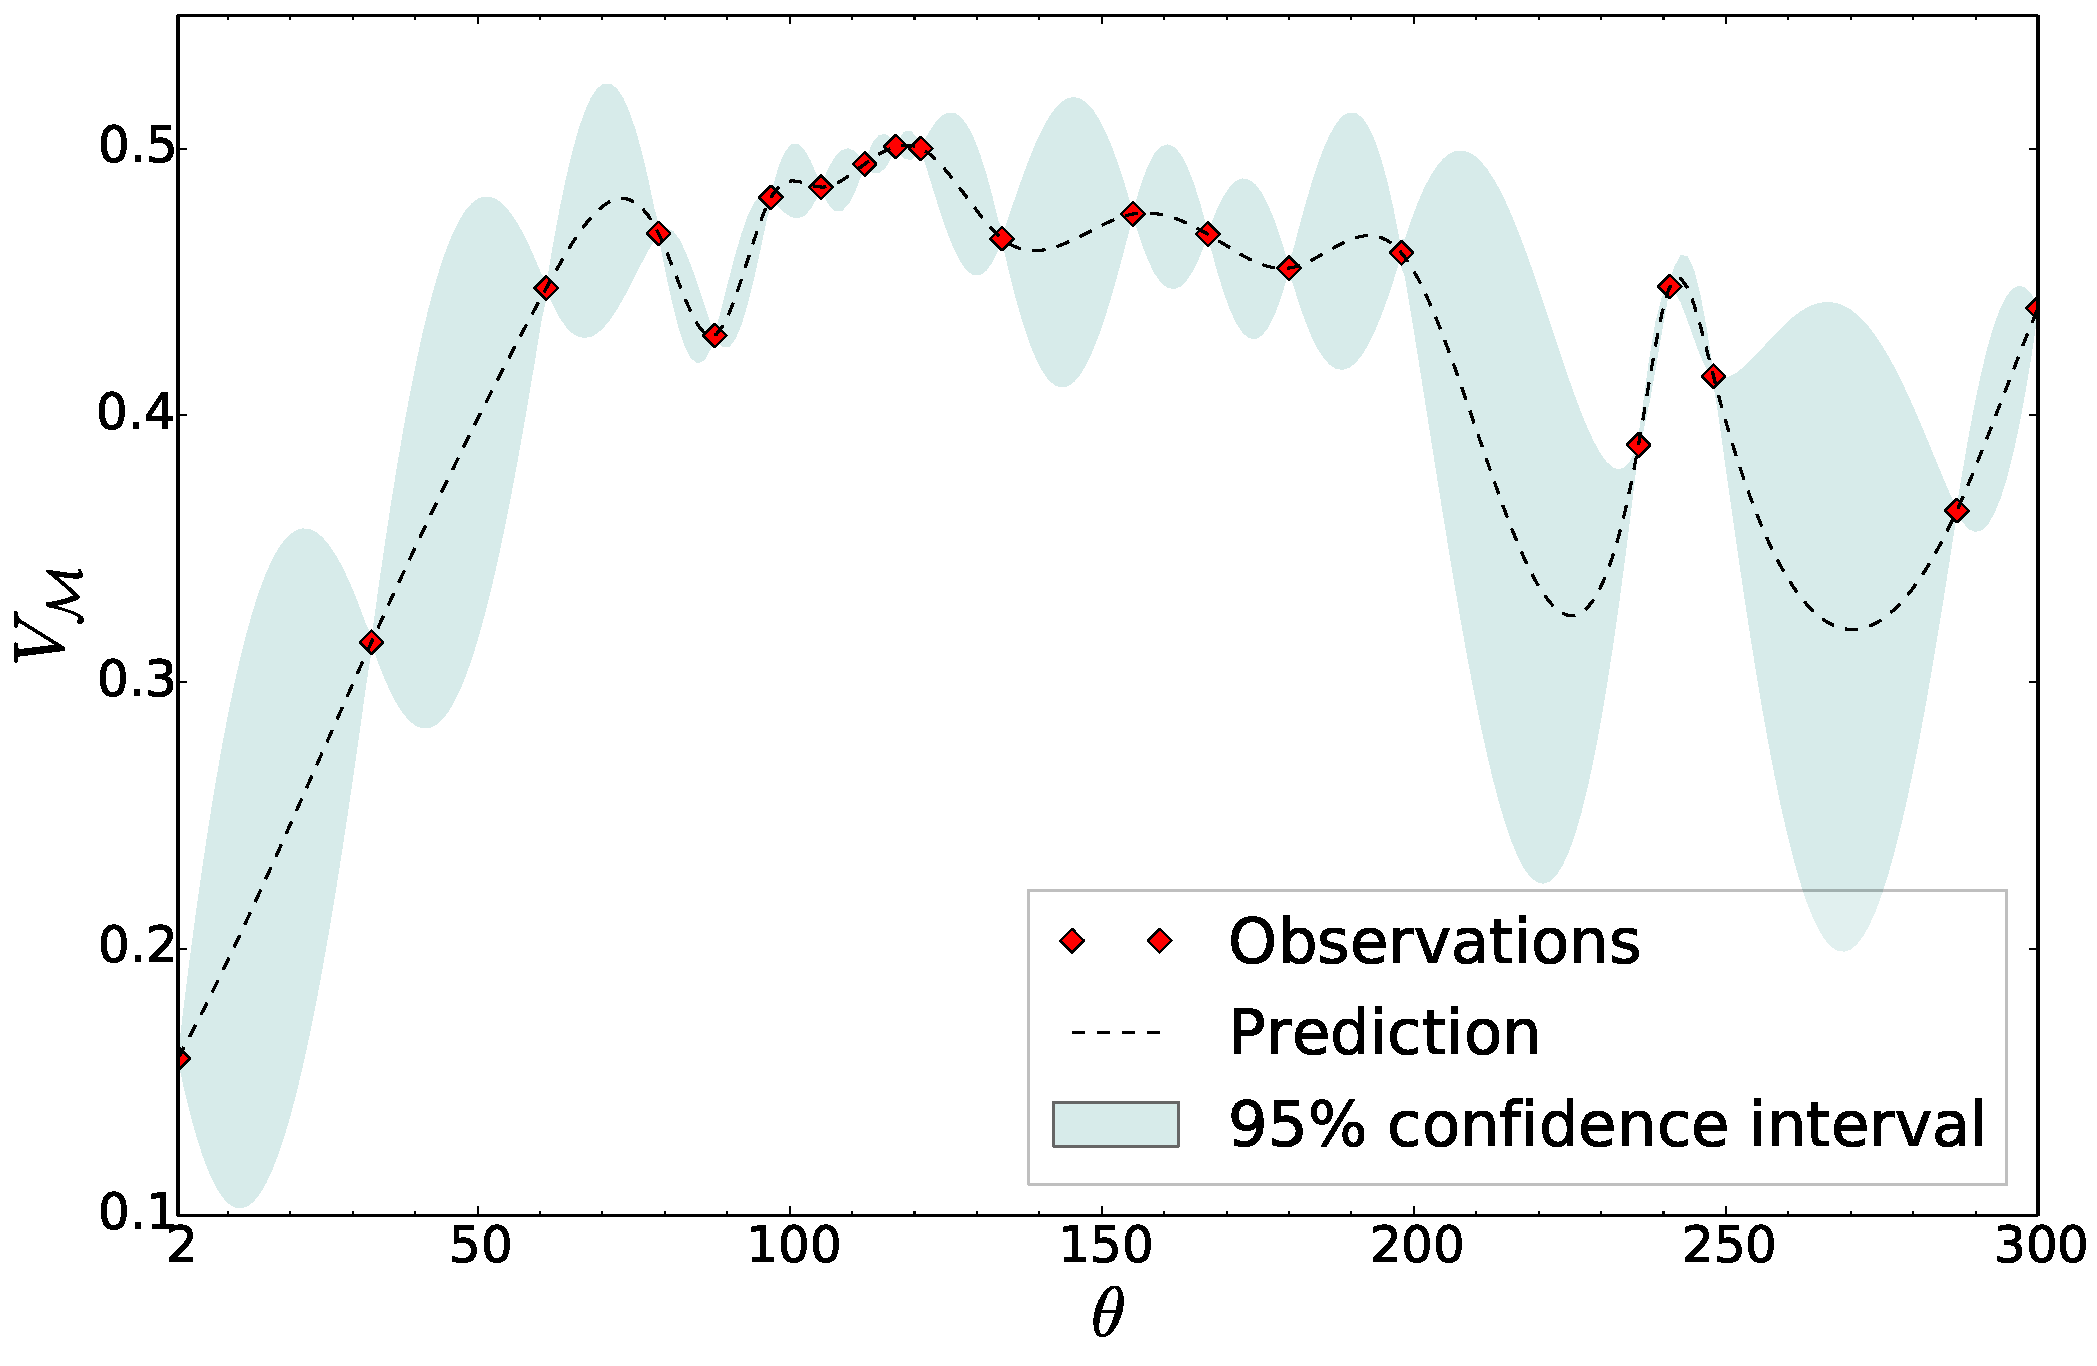
\includegraphics[width=\textwidth]{plots/tum_base/plot_b_05__alg_kmeans_pct_100_acq_ei}
		\caption{Experiment 9: Weight factor $\beta = 0.5$}
		\label{fig:exp9}
	\end{subfigure}
	\caption{Plots showing a comparison of the resulting \acrshort{acr:gp} posterior for varying settings of the $\beta$ factor. The plots correspond to 20 iterations of the base framework on the \texttt{tum\_kitchen} environment with $k$-Means clustering and \acrshort{acr:mei} acquisition used.}
	\label{fig:plots_tum_base_weight}
\end{figure}
	
Finally, we look at the influence of the weight factor $\beta$ for the small environment considering the plots of \autoref{fig:exp1}, \autoref{fig:exp8} and \autoref{fig:exp9}.
In this particular situation, one might benefit from weighing $V_\mathit{DTP}$ in the model value, as it could make a clearer distinction between values for different settings of $\theta$, because it cancels out part of the uncertainty from the simulations.
The intuition of why this works well for this particular environment can be elucidated by \autoref{fig:plots_tum_multi_acq}, which shows that the maxima of the $V_\mathit{DTP}$ and $V_\mathit{SIM}$ measures lie close together.
However, setting $\beta > 0$ might also lead to a bias in other environments, which is that, although $V_\mathit{DTP}$ may have high value, computed policies may not work well in the simulations or the real world.

\subsubsection{UOL BL Environment}

Let us next consider the results for the large \texttt{uol\_bl} environment. In \autoref{fig:plots_uol_base_acq} plots are shown for the experiments in which different acquisitions were used in the \acrshort{acr:bo}.
One can observe the optima found in each of these experiments lie close together.
The experiment that employs the \acrshort{acr:mei} function, however, appears ineffective to find the same global maximum in multiple repetitions.
All in all, the \acrshort{acr:gp-ucb} and especially the \acrshort{acr:mei-ps} function appear most effective in sampling parameter settings that result in \acrshortpl{acr:mdp} yielding high performance.

\afterpage{
\begin{figure}[!t]
	\centering
	\captionsetup{font=small}
	\captionsetup[subfigure]{font=footnotesize}
	\captionsetup[subfigure]{justification=centering}
	\begin{subfigure}[t]{0.65\textwidth}
		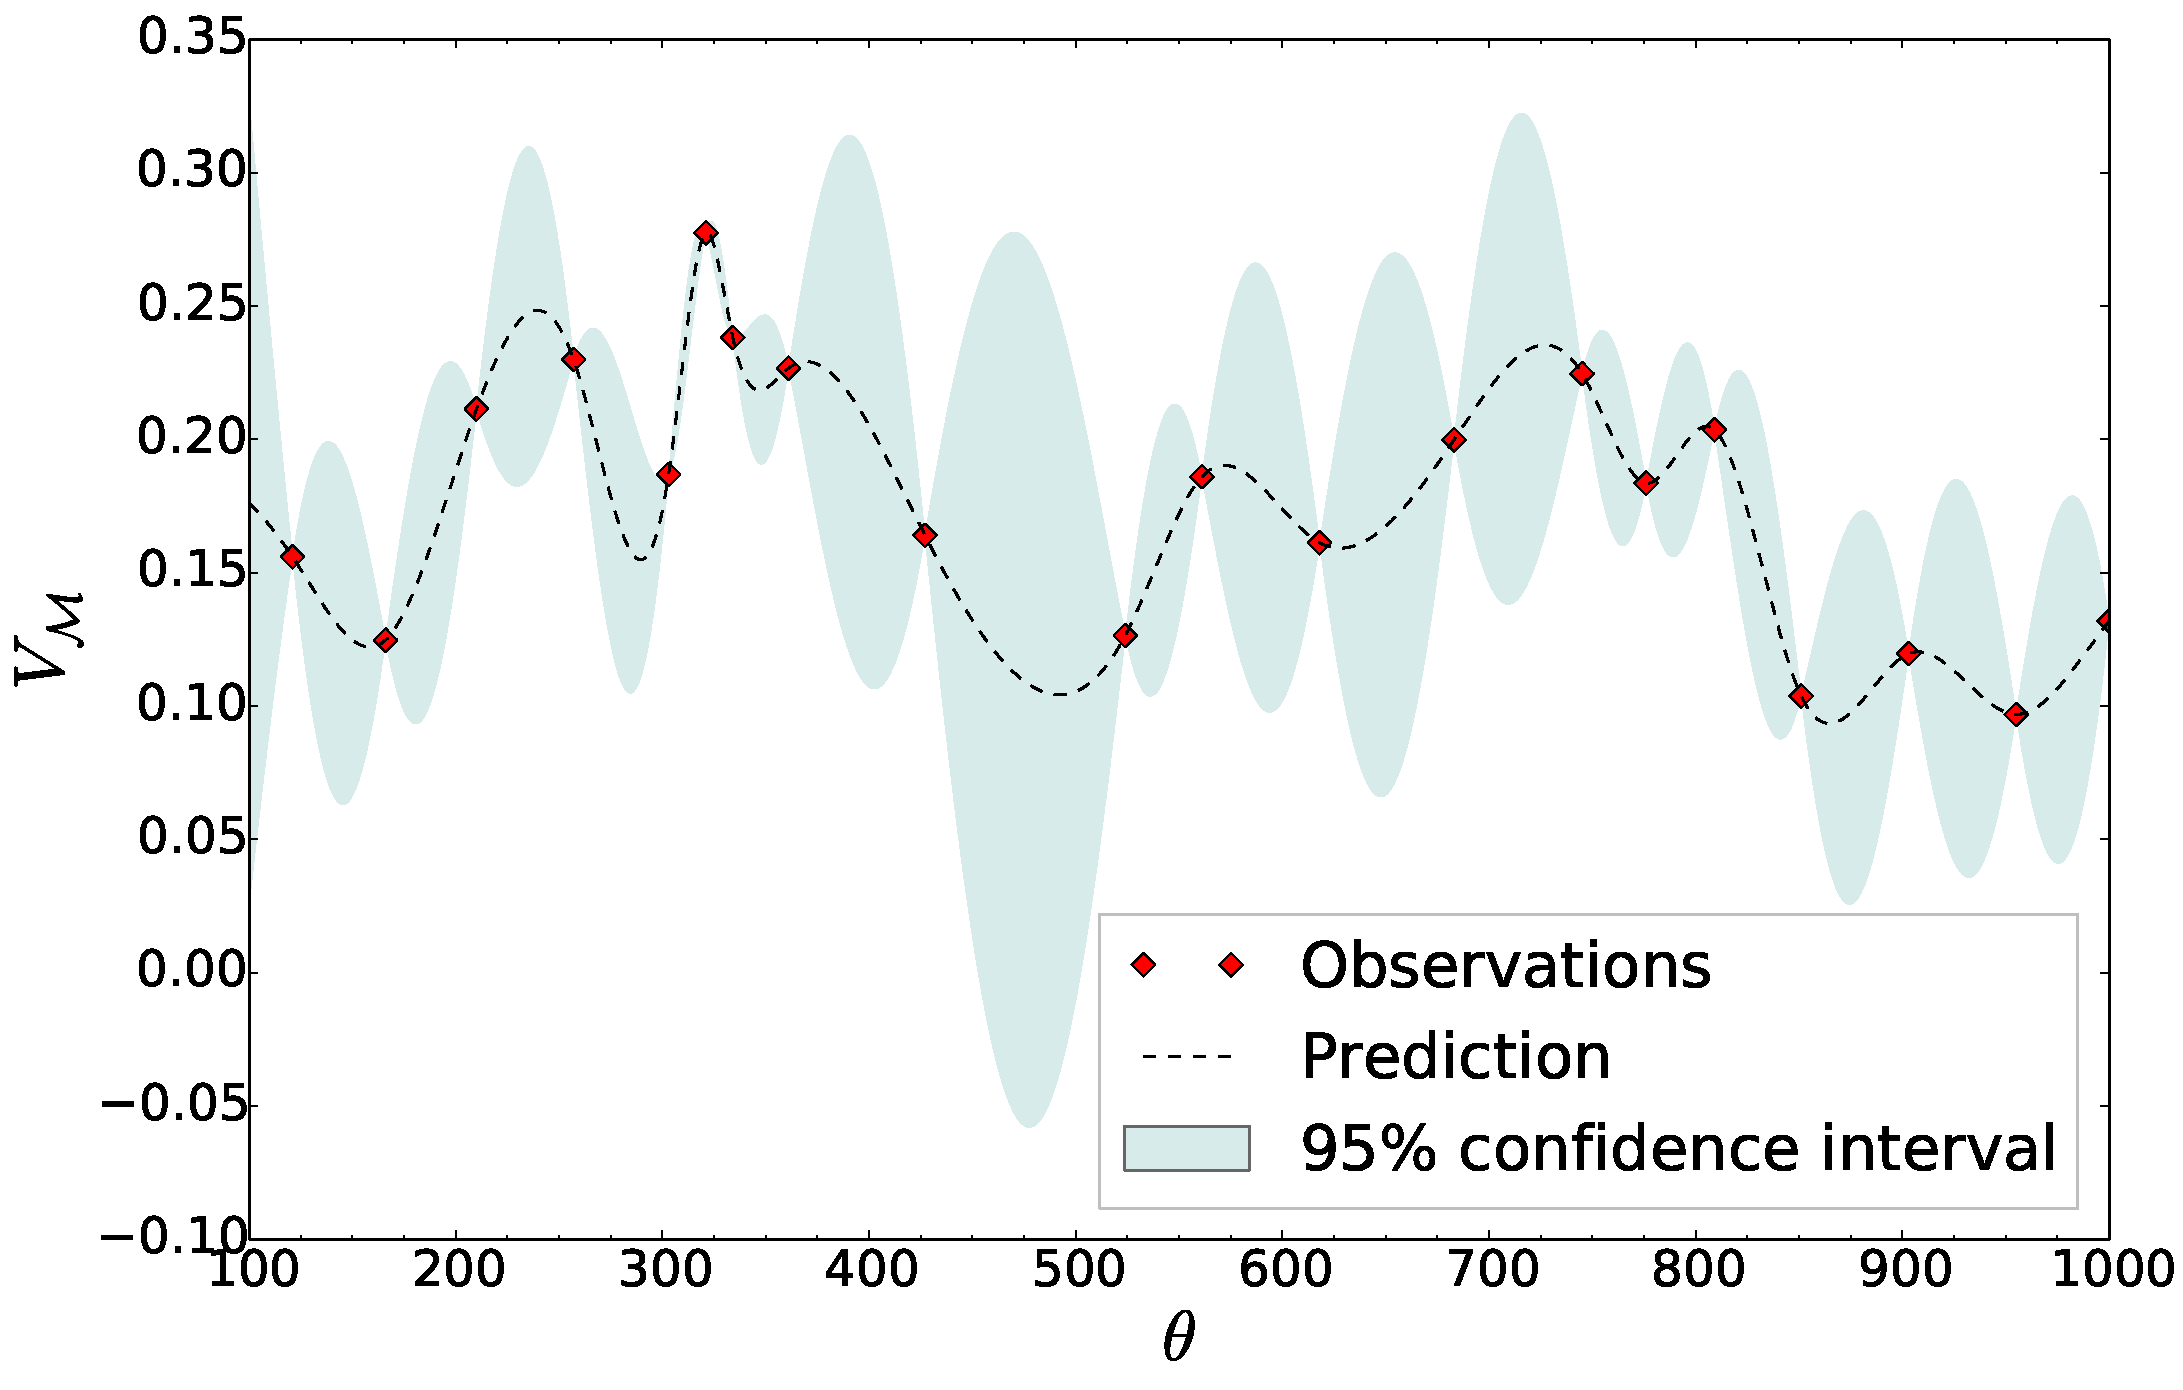
\includegraphics[width=\textwidth]{plots/uol_base/plot_b_00__alg_kmeans_pct_100_acq_ei}
		\caption{Experiment 10: \acrshort{acr:mei} acquisition function used}
		\label{fig:exp10}
	\end{subfigure}
	\bigskip
	
	\begin{subfigure}[t]{0.65\textwidth}
		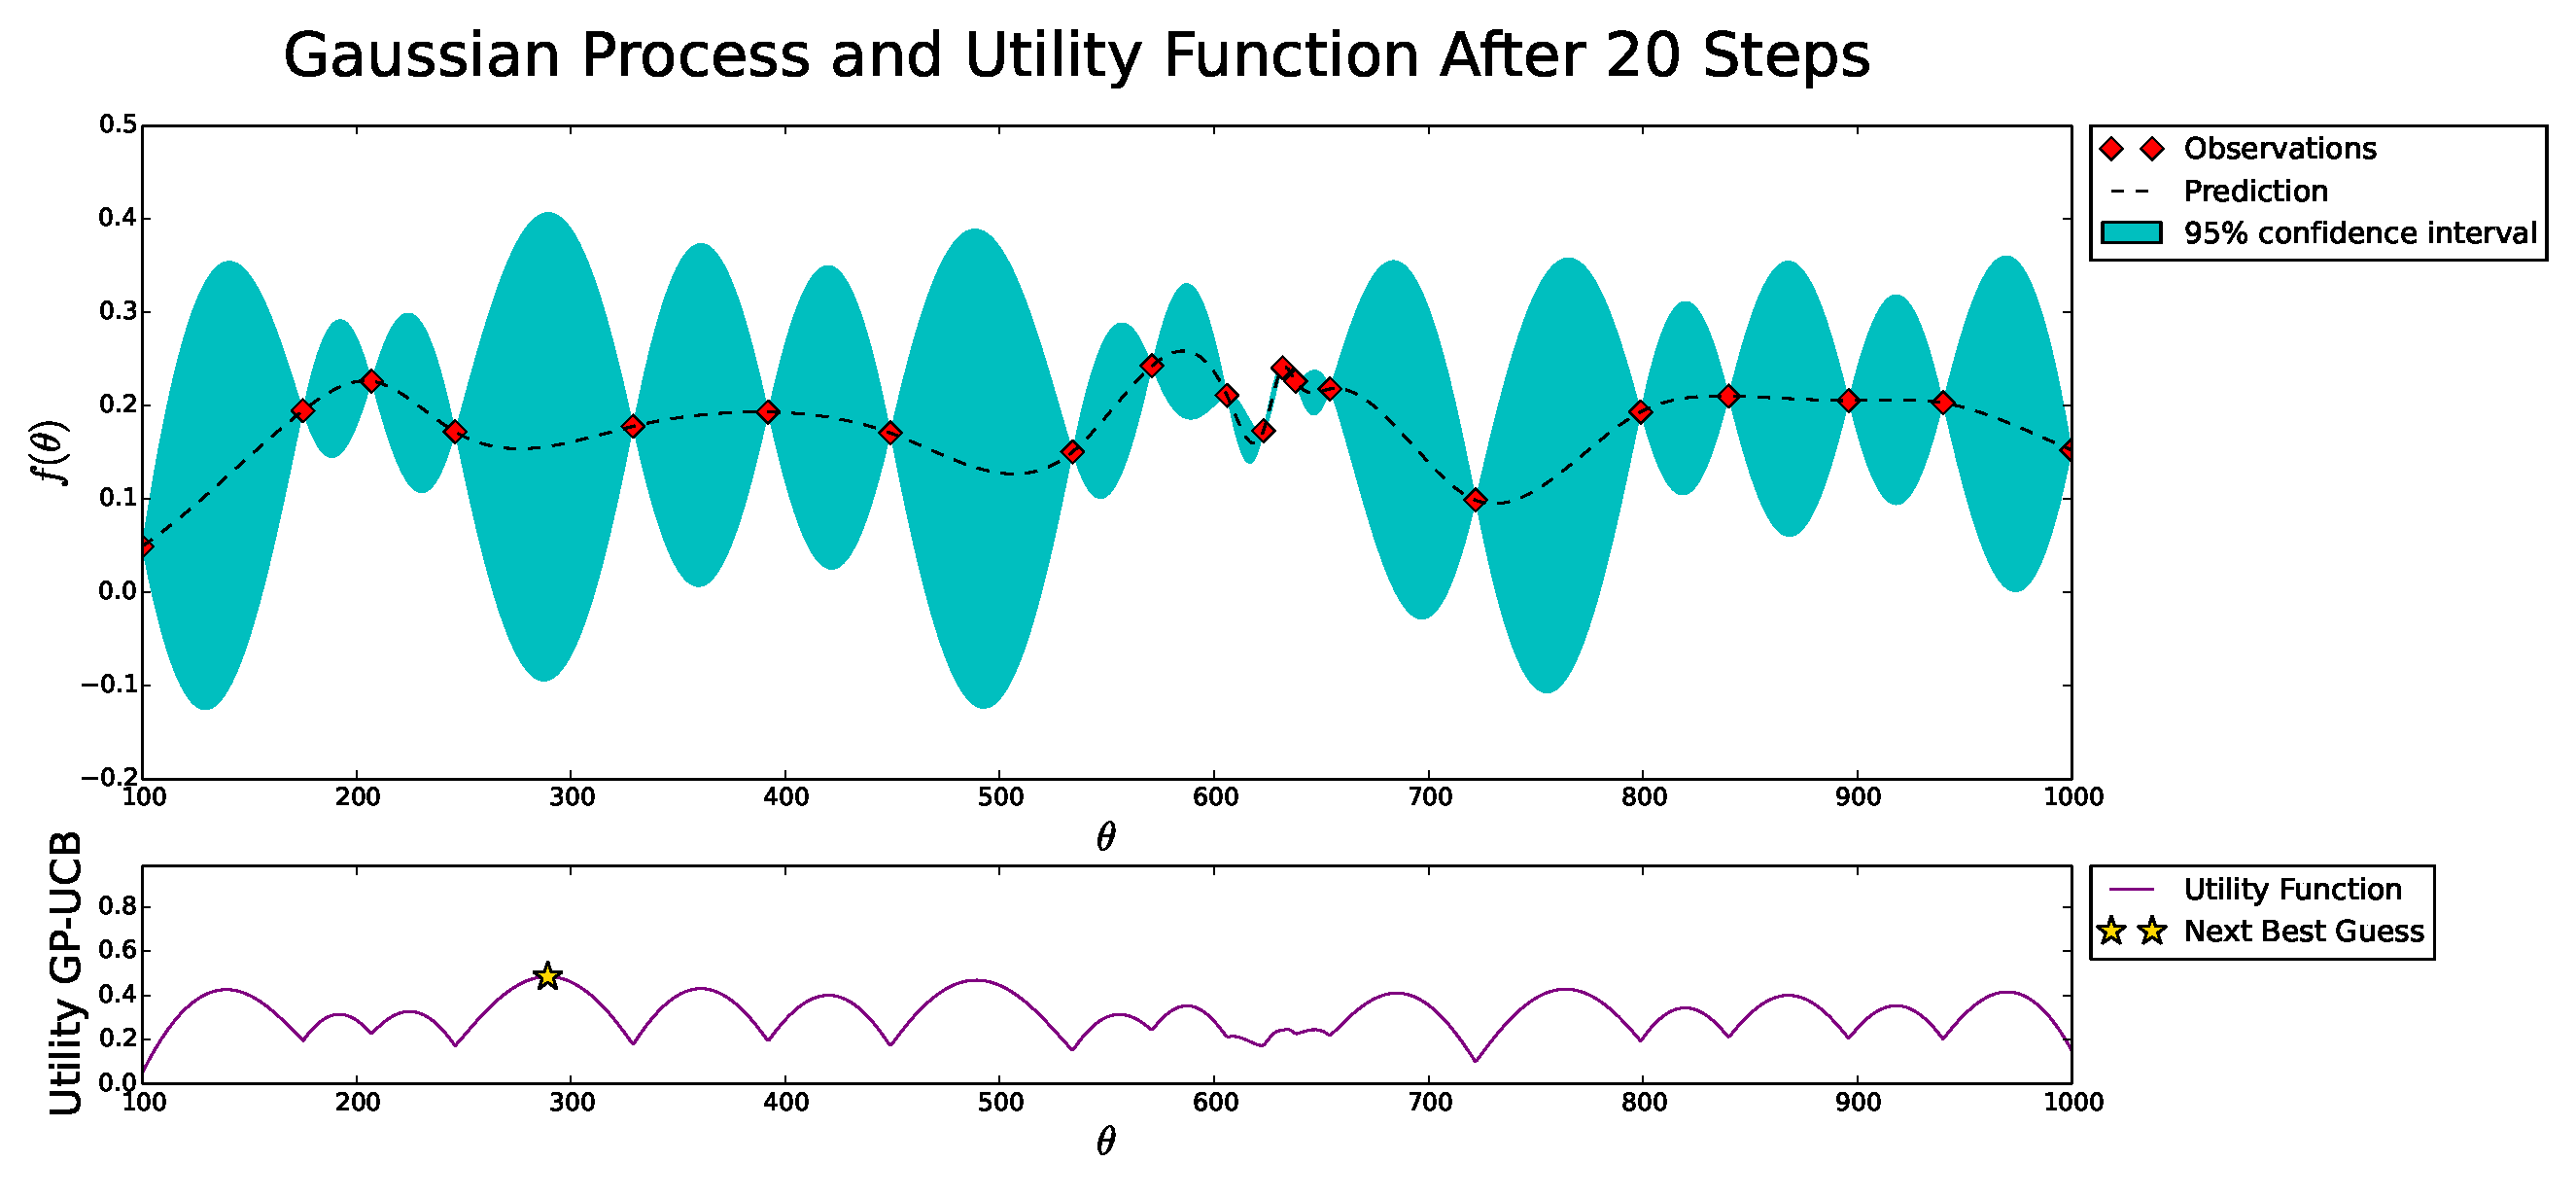
\includegraphics[width=\textwidth]{plots/uol_base/plot_b_00__alg_kmeans_pct_100_acq_ucb}
		\caption{Experiment 11: \acrshort{acr:gp-ucb} acquisition function used}
		\label{fig:exp11}
	\end{subfigure}
	\bigskip
	
	\begin{subfigure}[t]{0.65\textwidth}
		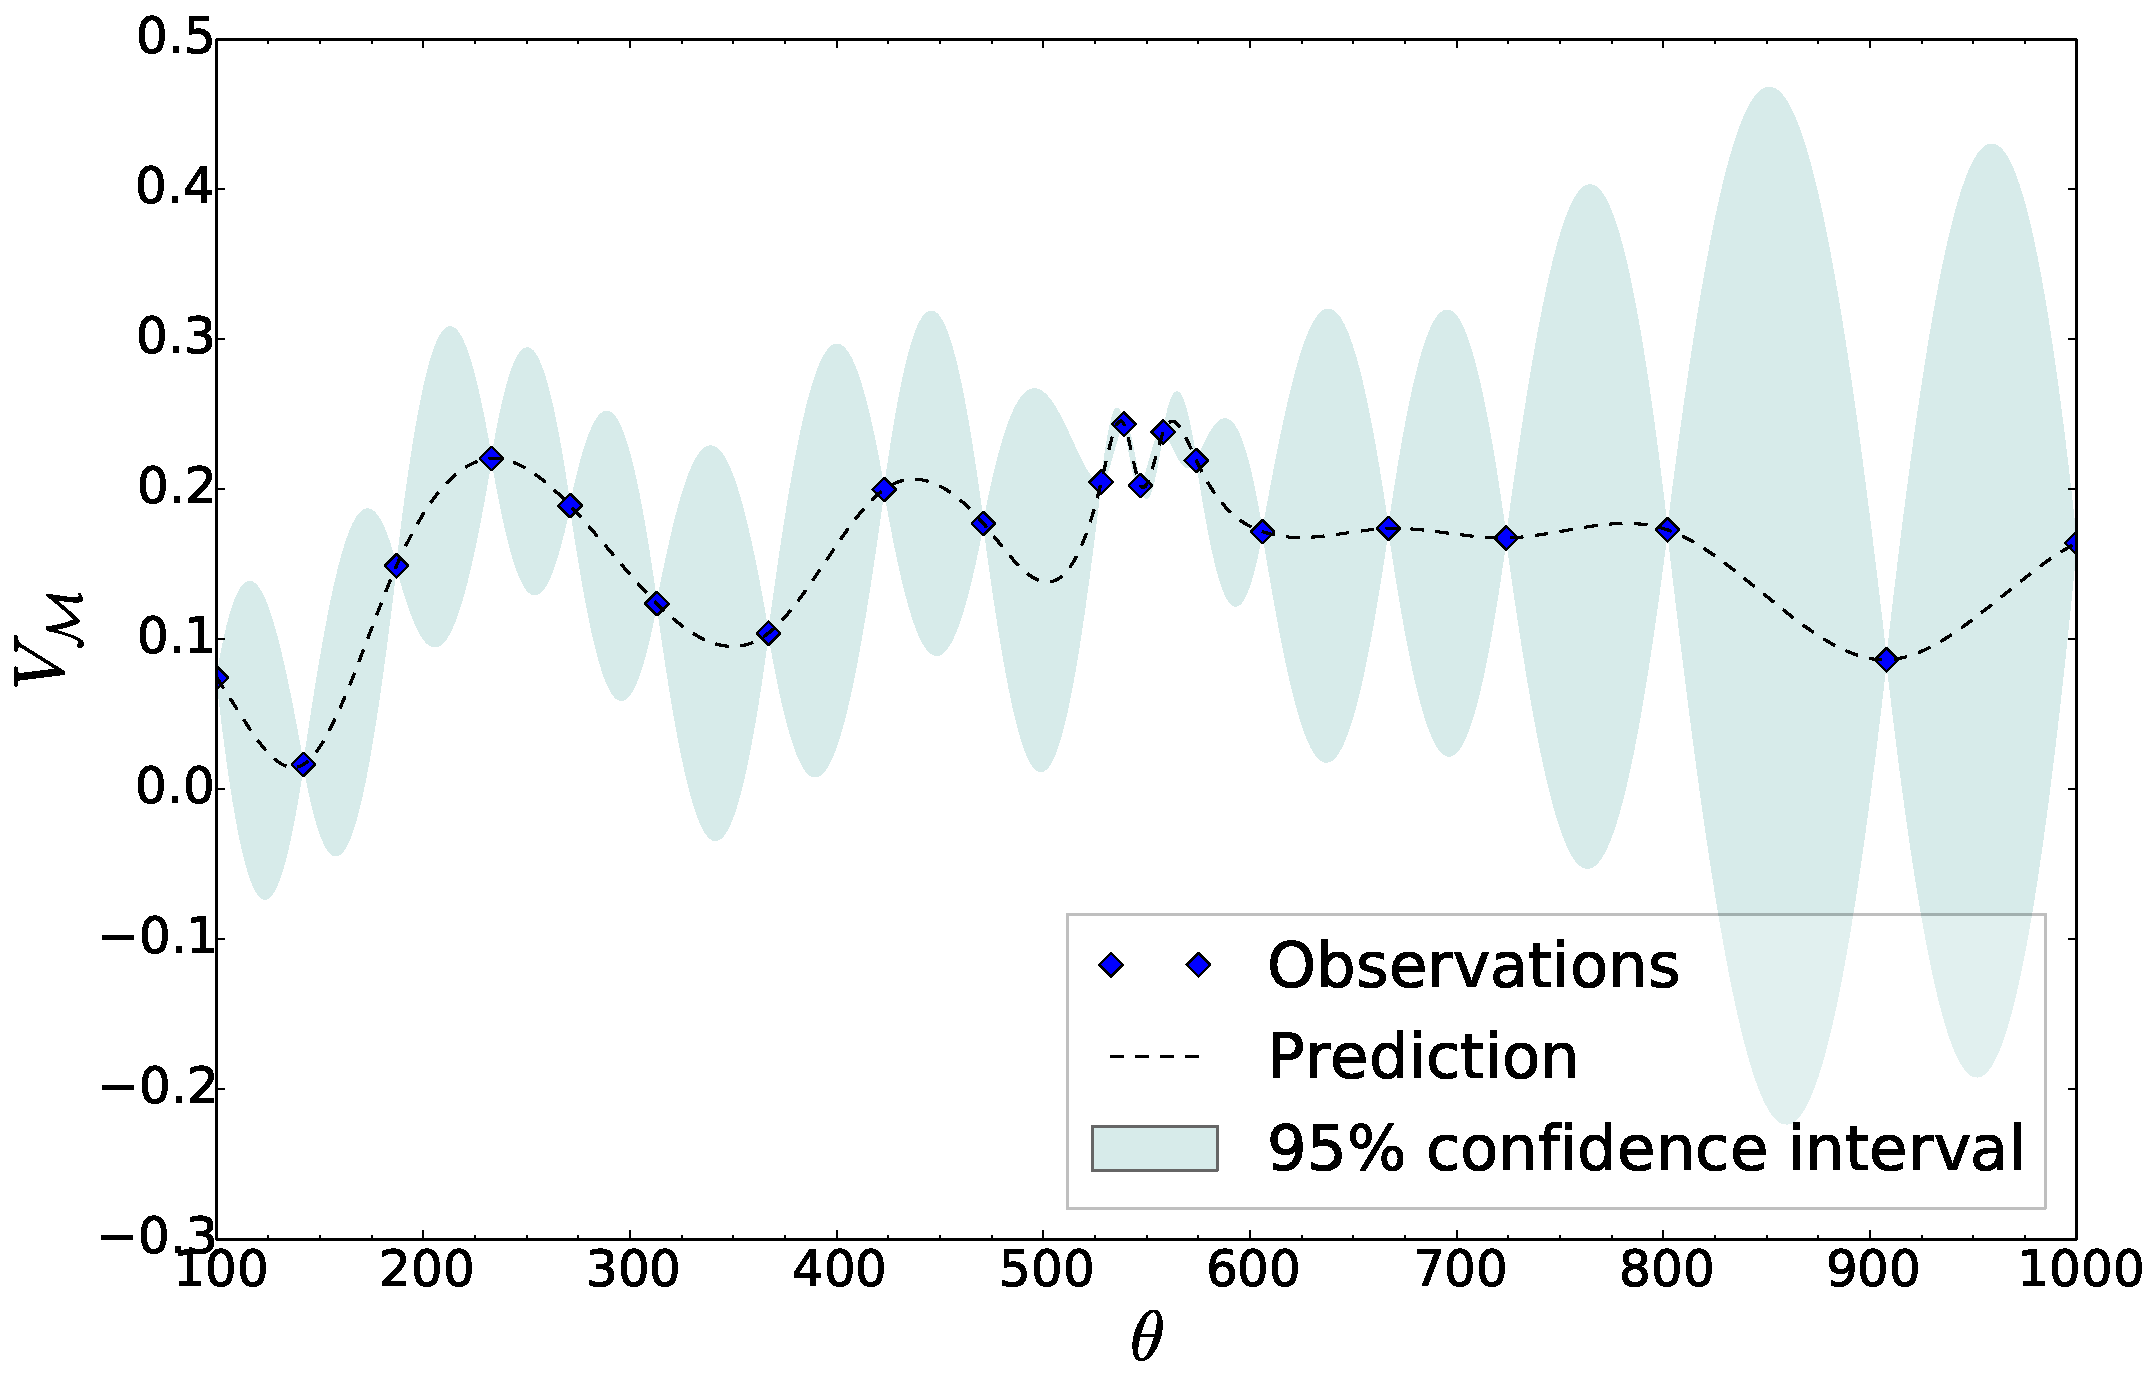
\includegraphics[width=\textwidth]{plots/uol_base/plot_b_00__alg_kmeans_pct_100_acq_eips}
		\caption{Experiment 12: \acrshort{acr:mei-ps} acquisition function used}
		\label{fig:exp12}
	\end{subfigure}
	\bigskip
	\caption{Plots showing a comparison of the resulting \acrshort{acr:gp} posterior for varying acquisition functions. The plots correspond to the \texttt{uol\_bl} environment with $\beta = 0.0$ and $k$-Means~clustering~used.}
	\label{fig:plots_uol_base_acq}
\end{figure}
\clearpage
}

\newpage

\begin{figure}[!t]
	\centering
	\captionsetup{font=small}
	\captionsetup[subfigure]{font=footnotesize}
	\captionsetup[subfigure]{justification=centering}
	\begin{subfigure}[t]{0.495\textwidth}
		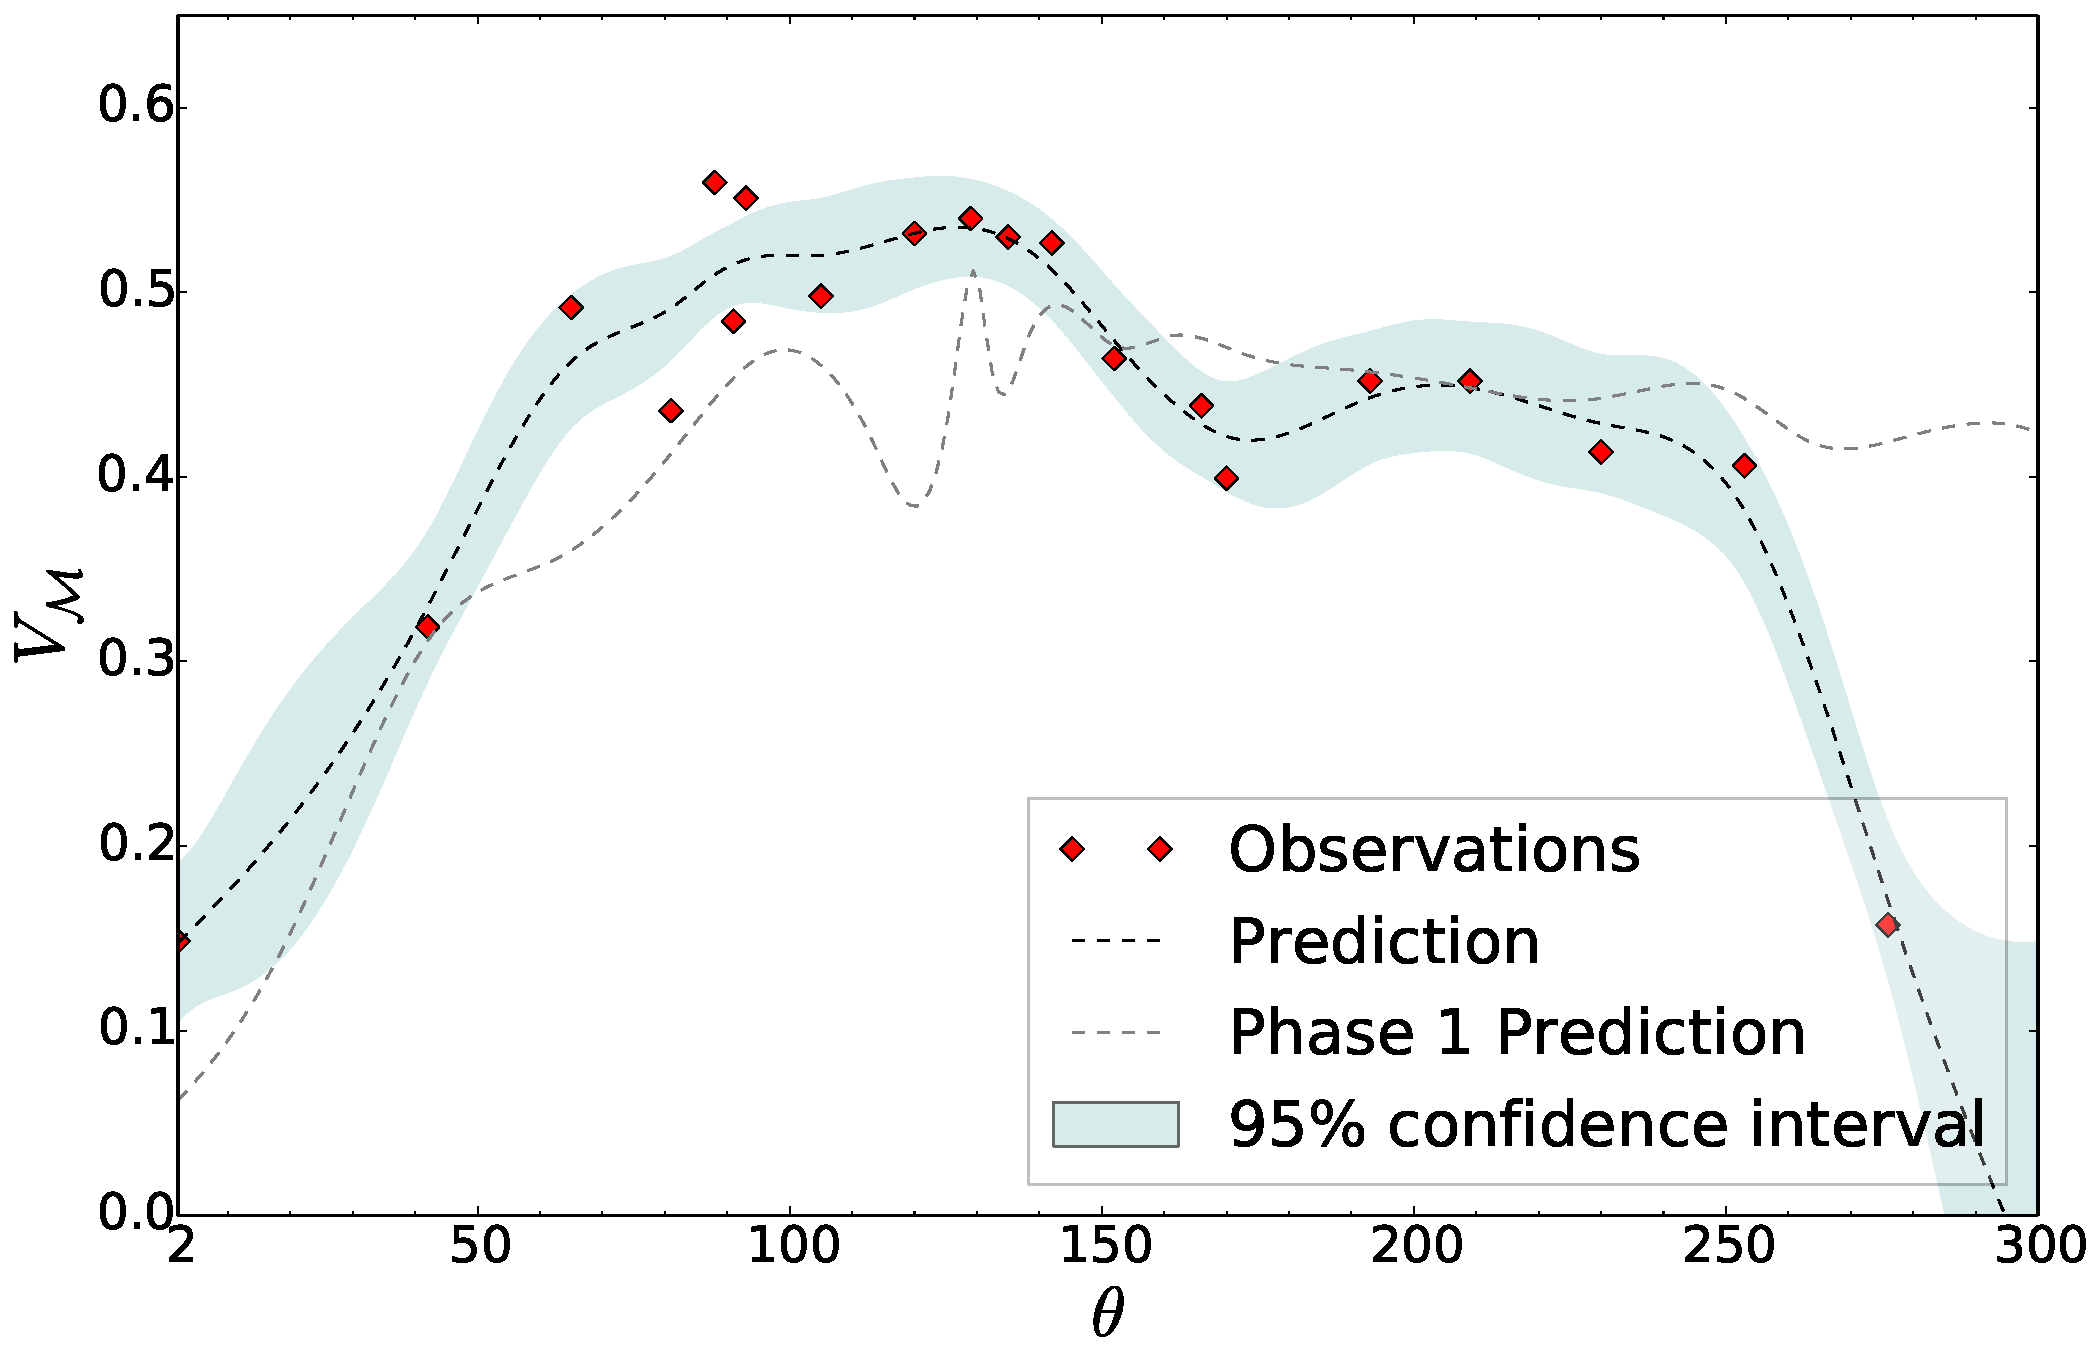
\includegraphics[width=\textwidth]{plots/tum_multi/plot_b_00__alg_kmeans_pct_100_acq_ei}
		\caption{Experiment 13: \acrshort{acr:mei} acquisition function in phase 1}
		\label{fig:exp13}
	\end{subfigure}
	\begin{subfigure}[t]{0.495\textwidth}
		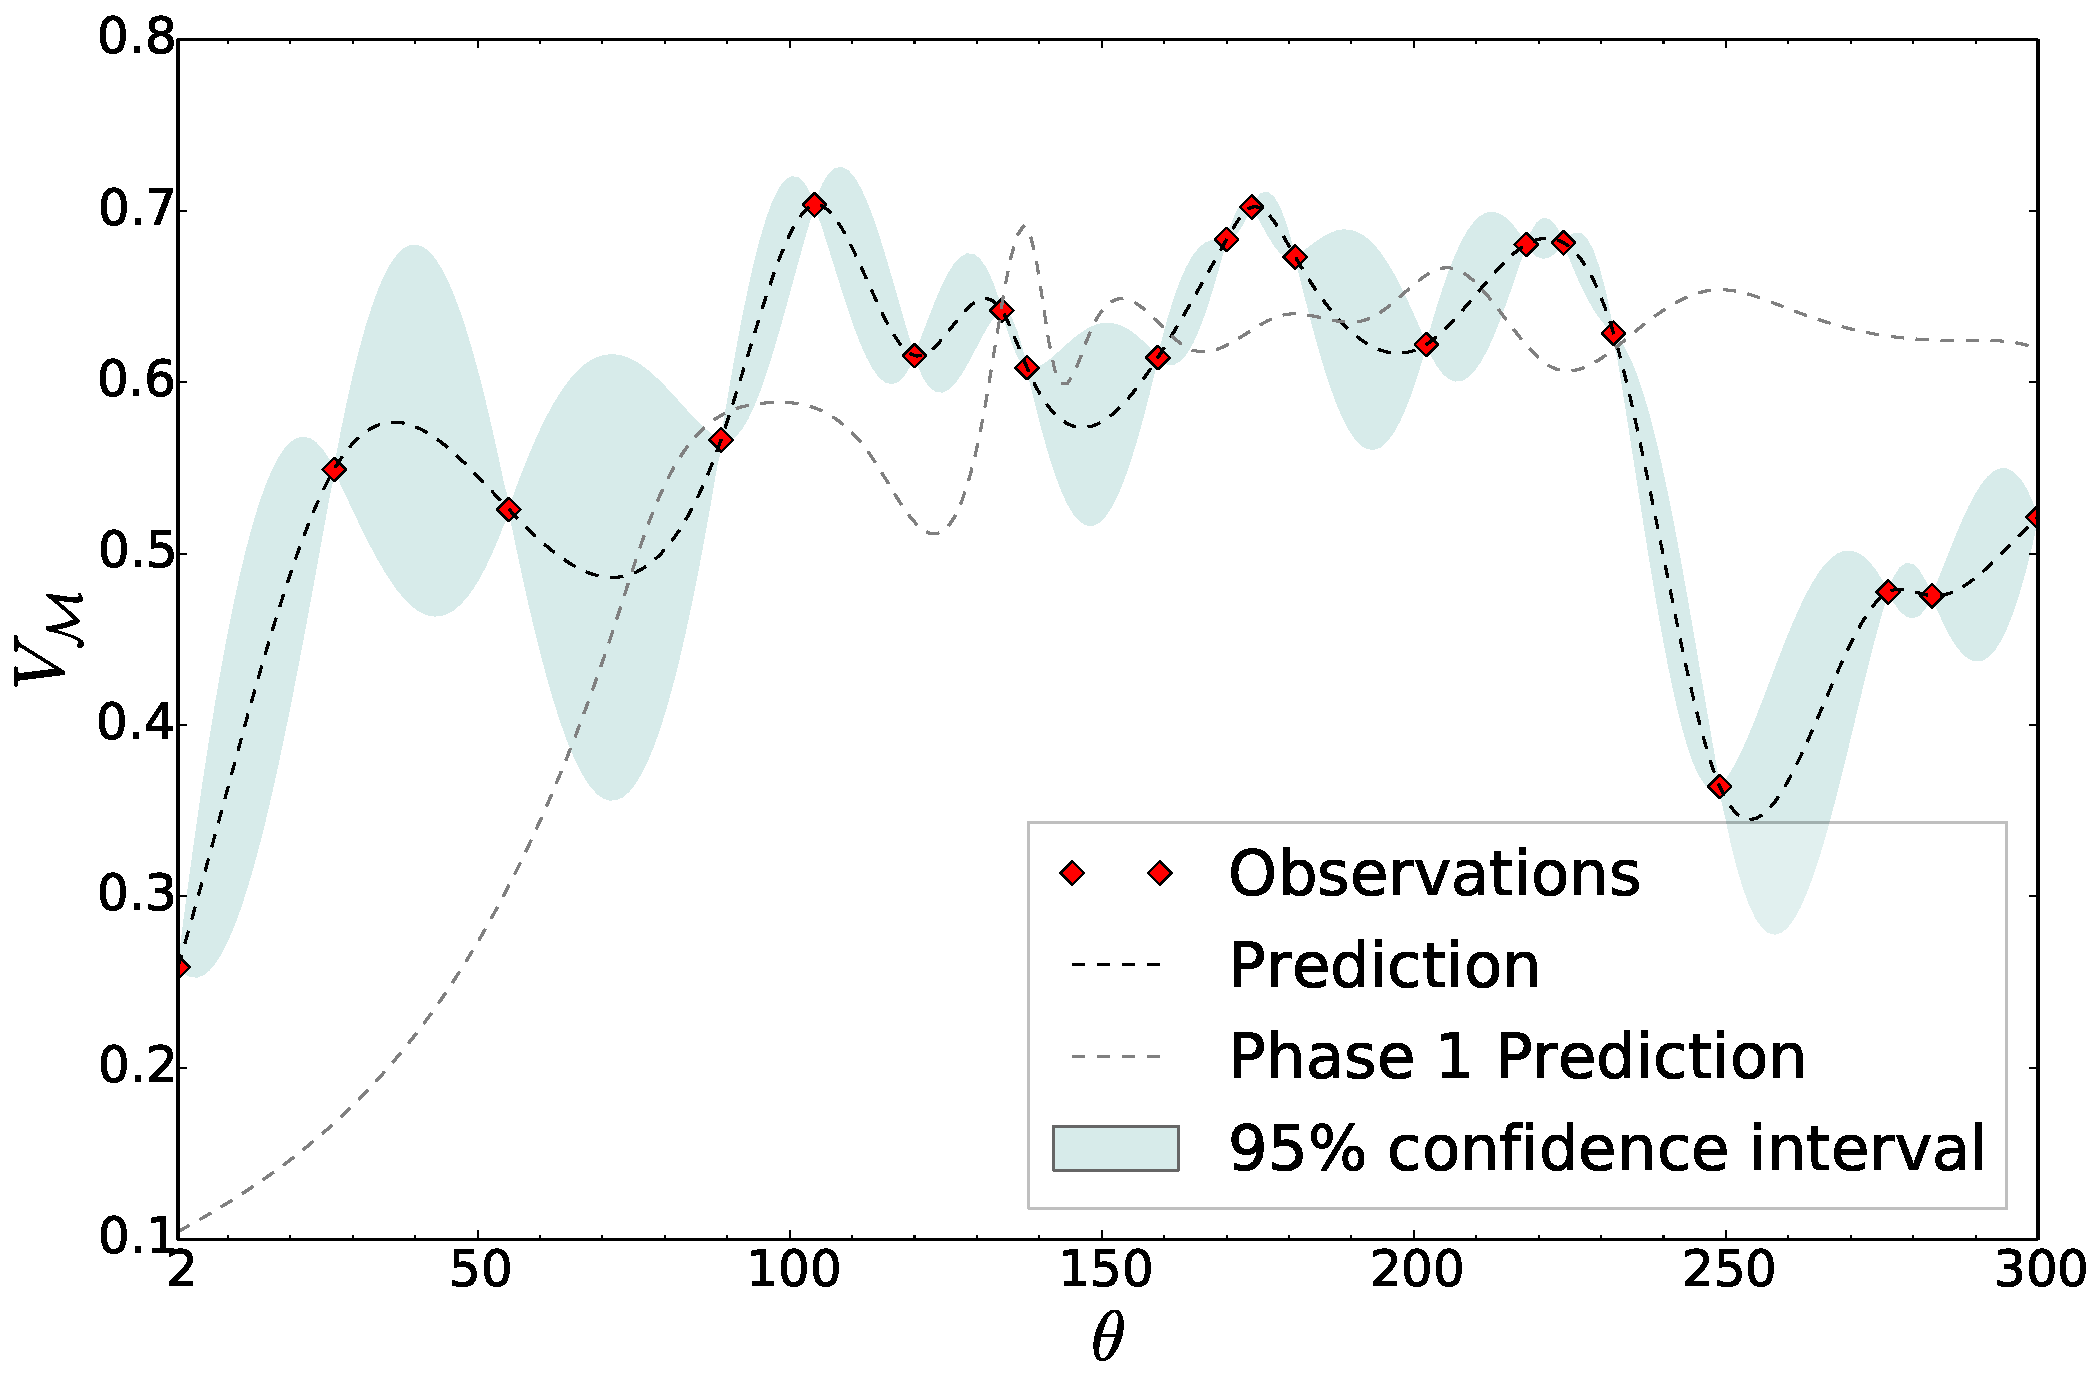
\includegraphics[width=\textwidth]{plots/tum_multi/plot_b_00__alg_kmeans_pct_100_acq_ucb}
		\caption{Experiment 14: \acrshort{acr:gp-ucb} acquisition function in phase 1}
		\label{fig:exp14}
	\end{subfigure}
	\caption{Plots showing a comparison of the resulting \acrshort{acr:gp} posterior for varying acquisition functions. The plots correspond to 20 iterations of the multi-phase framework on the \texttt{tum\_kitchen} environment with $\beta = 0.0$ and $k$-Means~clustering~used.}
	\label{fig:plots_tum_multi_acq}
	
	\null
	\begin{subfigure}[t]{0.495\textwidth}
		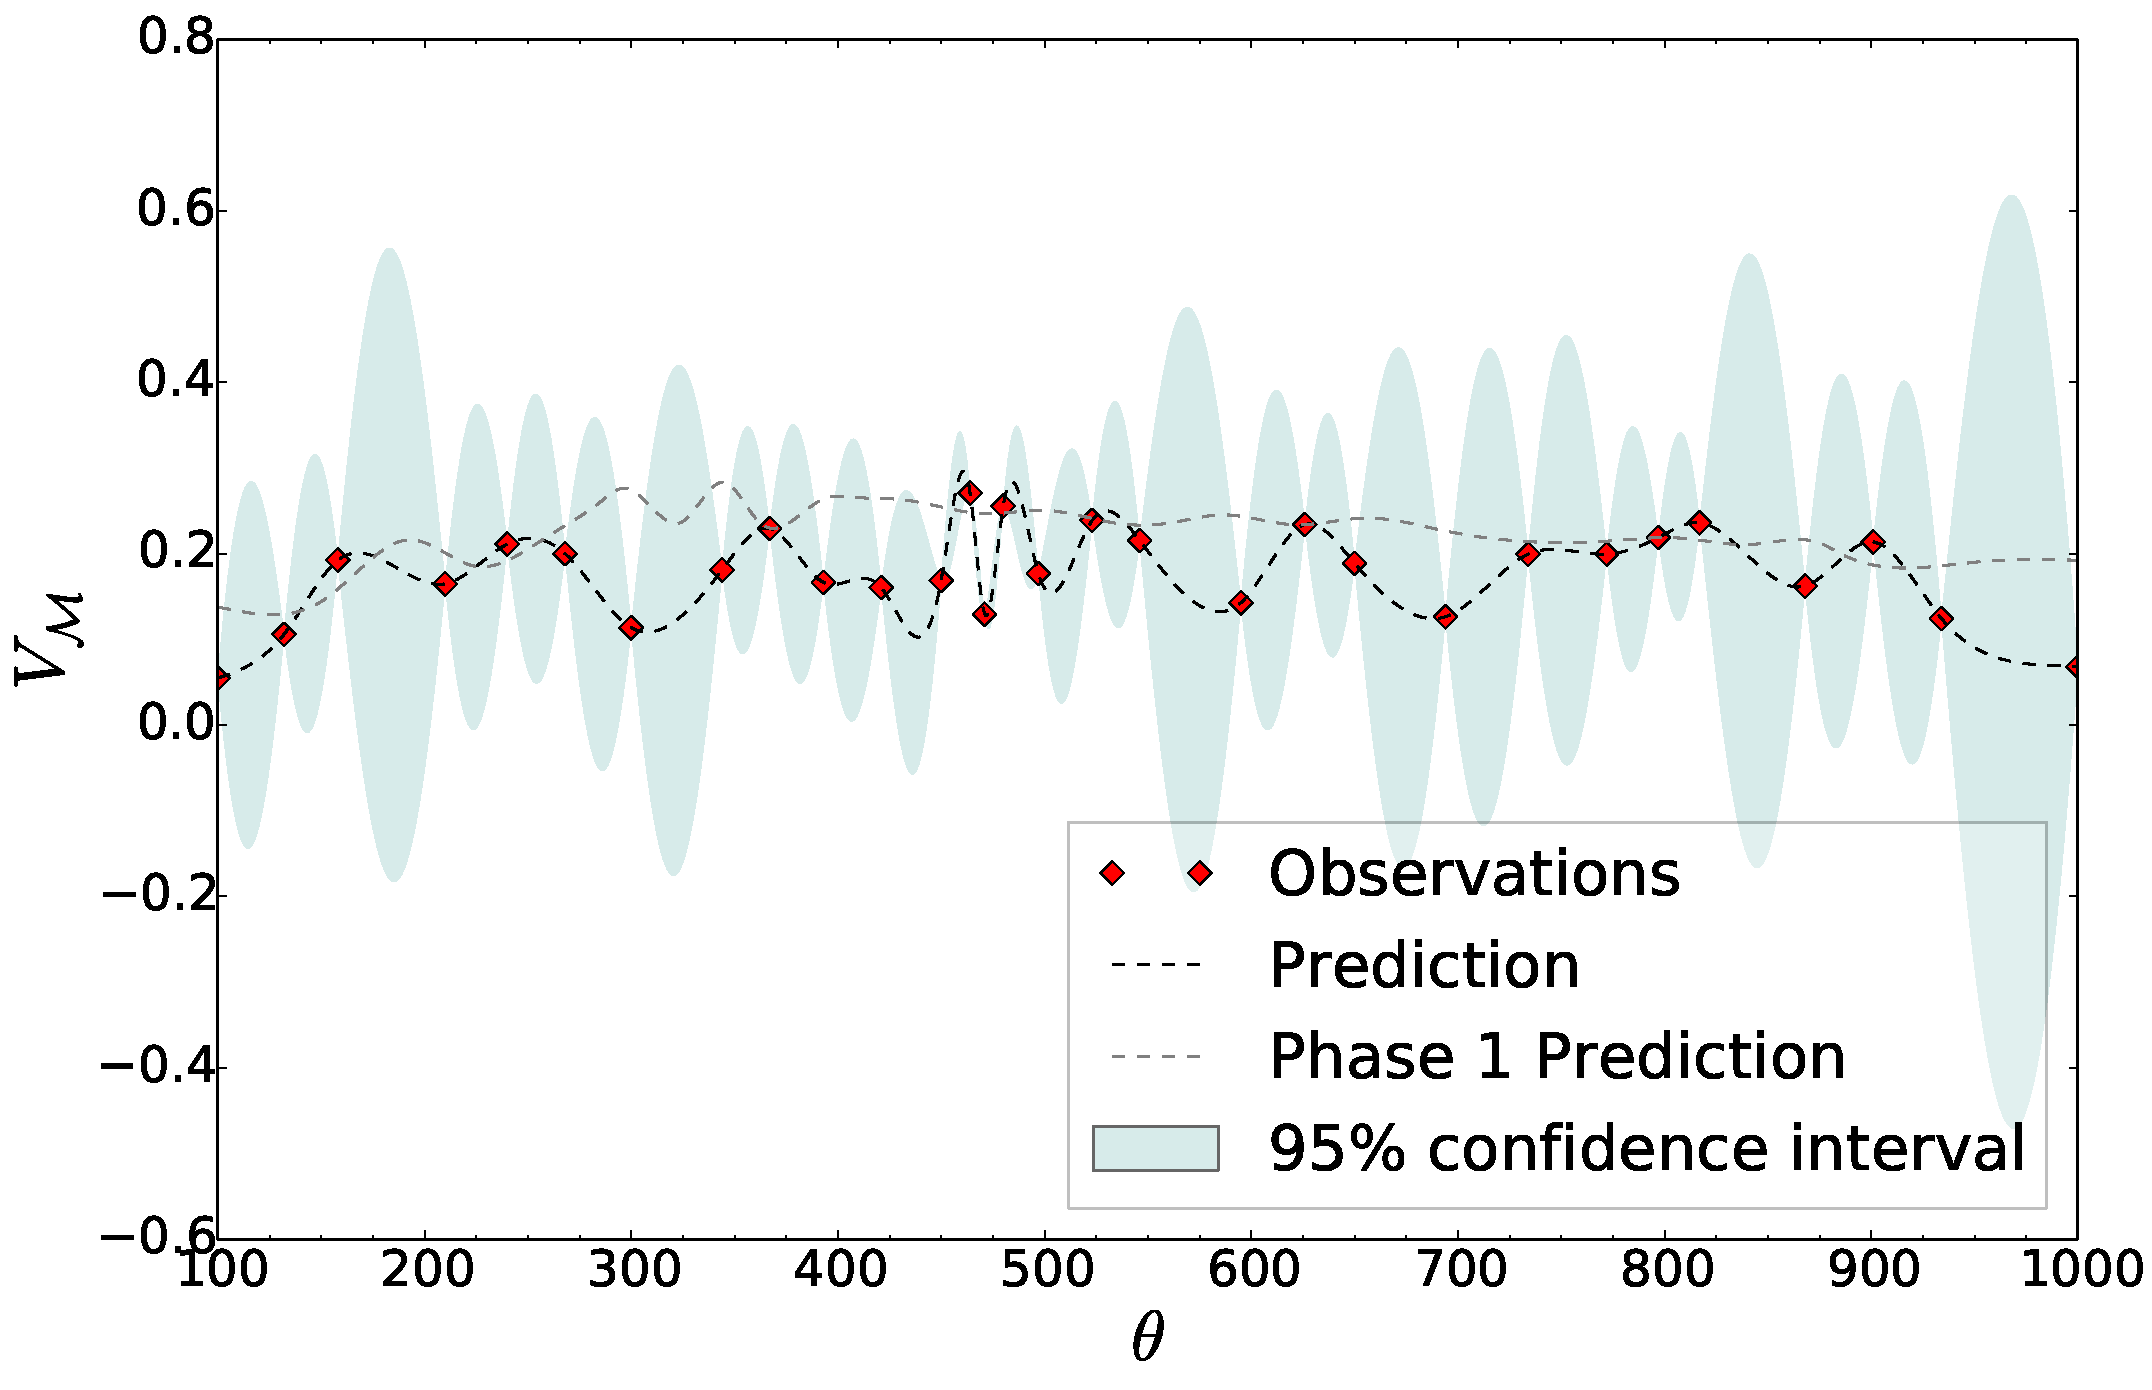
\includegraphics[width=\textwidth]{plots/uol_multi/plot_b_00__alg_kmeans_pct_100_acq_ei}
		\caption{Experiment 15: \acrshort{acr:mei} acquisition function in phase 1}
		\label{fig:exp15}
	\end{subfigure}
	\begin{subfigure}[t]{0.495\textwidth}
		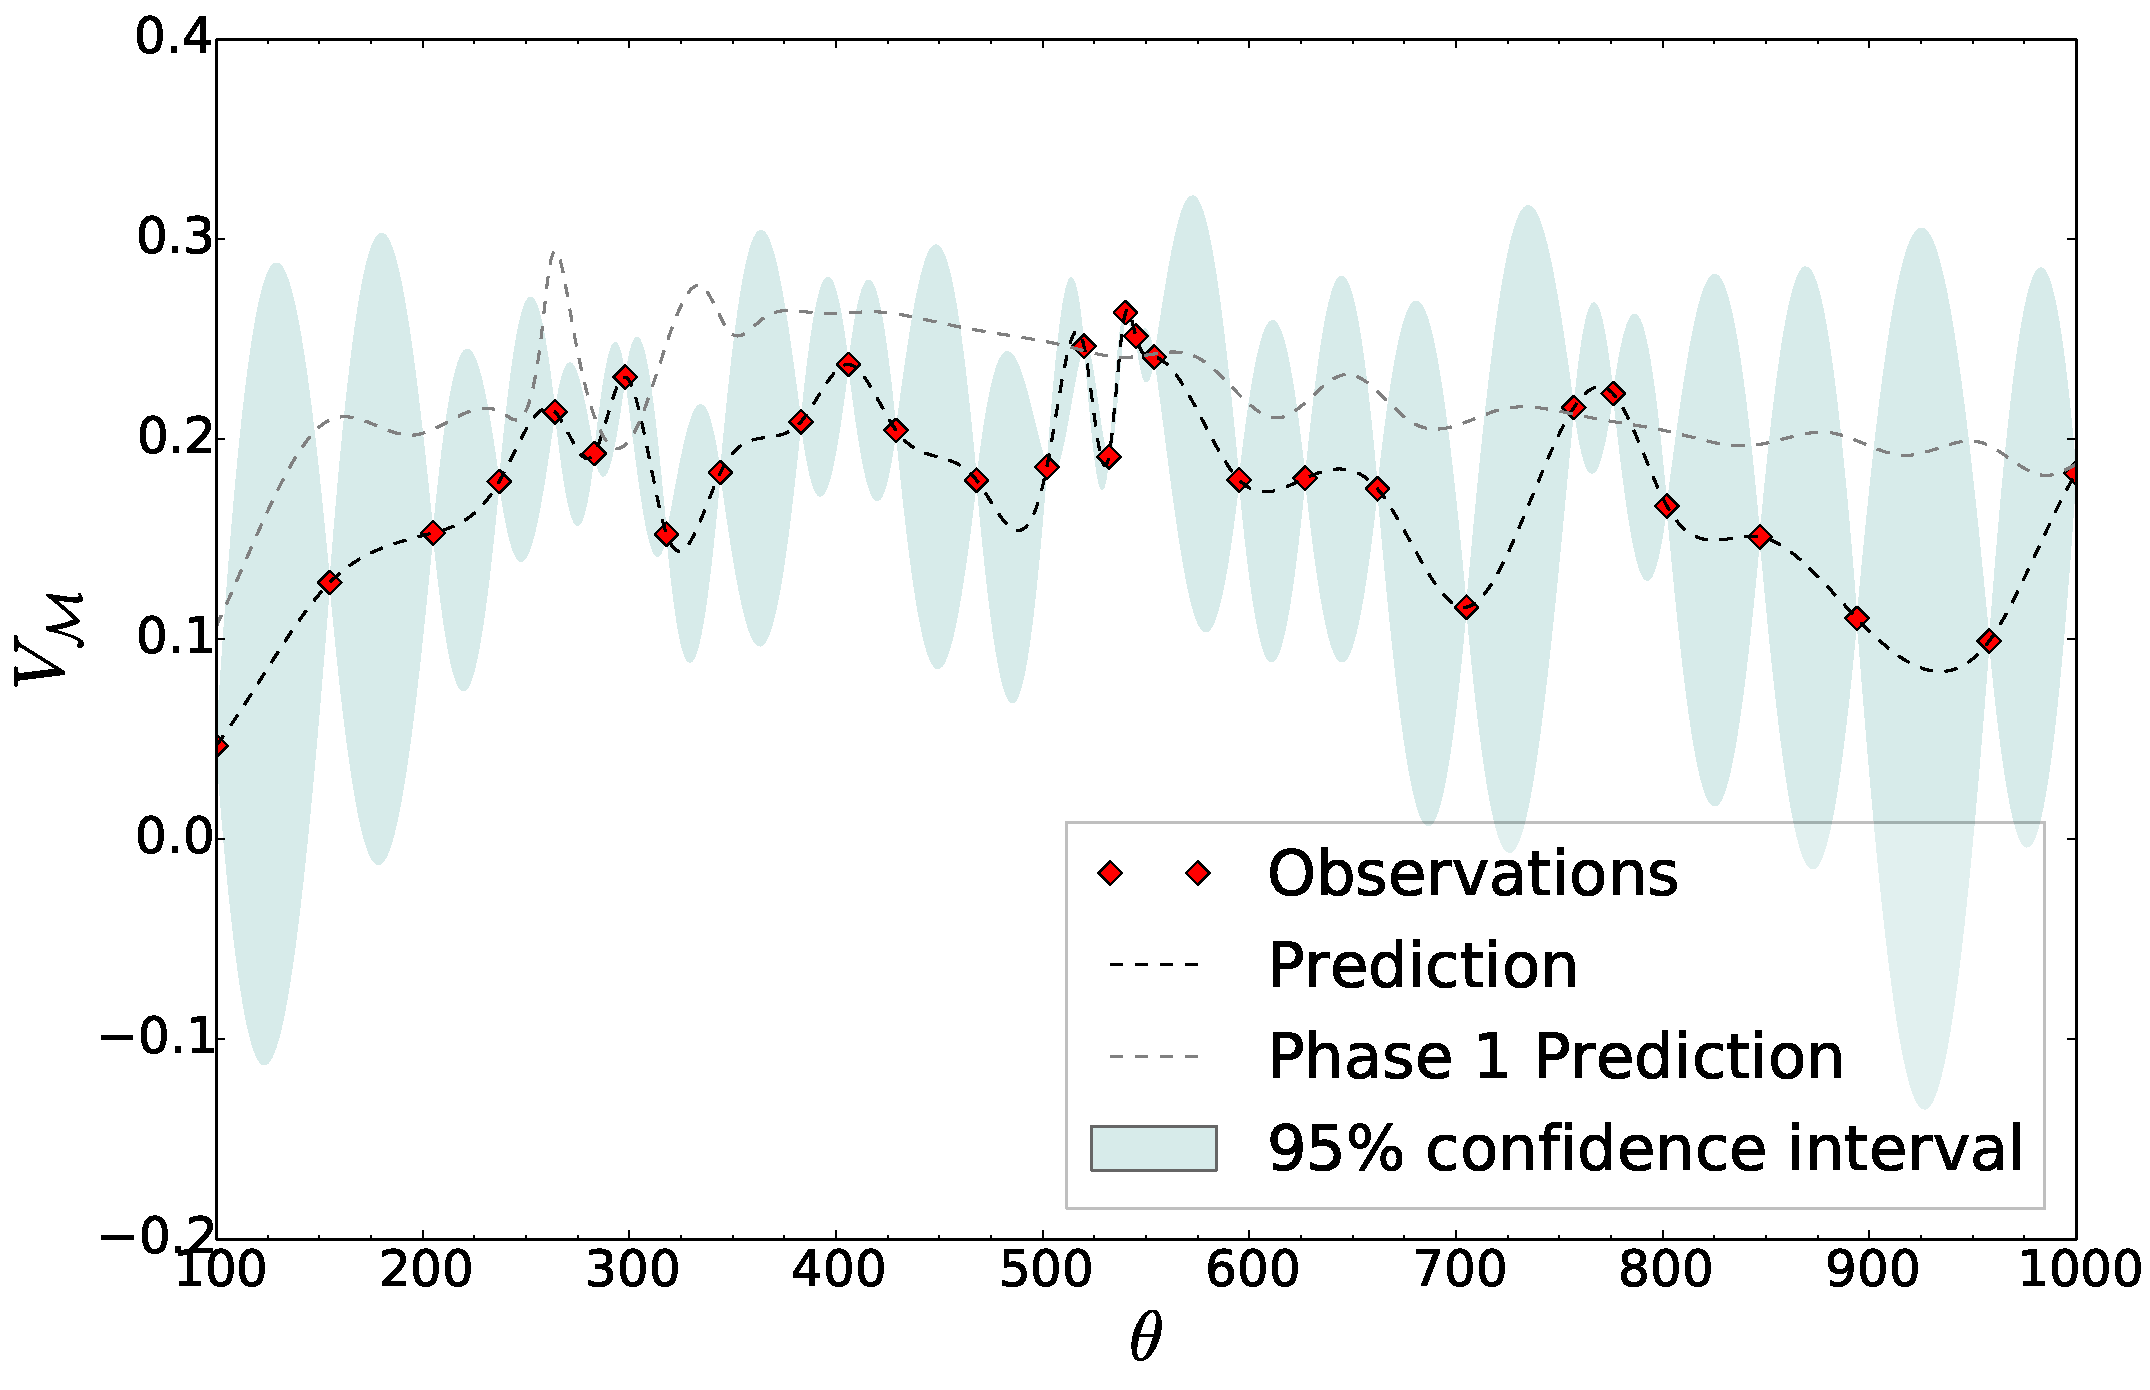
\includegraphics[width=\textwidth]{plots/uol_multi/plot_b_00__alg_kmeans_pct_100_acq_ucb}
		\caption{Experiment 16: \acrshort{acr:gp-ucb} acquisition function in phase 1}
		\label{fig:exp16}
	\end{subfigure}
	\caption{Plots showing a comparison of the resulting \acrshort{acr:gp} posterior for varying acquisition functions. The plots correspond to 30 iterations of the multi-phase framework on the \texttt{uol\_bl} environment with $\beta = 0.0$ and $k$-Means~clustering~used.}
	\label{fig:plots_uol_multi_acq}
\end{figure}

\begin{table}[t!]
	\centering
	\caption{Overview of the time expenses of a single iteration for model learning, planning and simulation with the algorithms used in the experiments. The time expenses are presented as ranges for the smallest and largest \acrshortpl{acr:mdp} learned for the environment.}
	\label{tab:framework-time-expenses}
	\begin{tabular}{|l|r|r|r|}
		\hline
		\textbf{Environment}    & \textbf{Model Learning Time (\si{\second})} & \textbf{Planning Time (\si{\second})} & \textbf{Simulation Time (\si{\second})} \\ \hline
		\texttt{tum\_kitchen} & \numrange[range-phrase = --]{0.2}{15.0}       & \numrange[range-phrase = --]{0.01}{0.5} & \numrange[range-phrase = --]{110}{200}                         \\ \hline
		\texttt{uol\_bl}      & \numrange[range-phrase = --]{1.0}{60.0}       & \numrange[range-phrase = --]{0.05}{5.0}   & \numrange[range-phrase = --]{100}{700}                        \\ \hline
	\end{tabular}
\end{table}

\subsection{Multi-Phase Framework}
\label{sec:multiphase-framework-results}

%In \Crefrange{fig:exp13}{fig:exp16} one can see that optima are found within the same area of the parameter space as seen in the results for the base framework.
Next, we present and evaluate our results obtained in the experiments on the multi-phase framework, for which the configurations are presented in \autoref{tab:configurations-multi}.
In these experiments, first an optimization takes place of the model value computed solely from the value functions for the tasks the system is expected perform.
Only computing the value functions for \acrshortpl{acr:mdp} as is done in this first phase is relatively time-cheap (i.e., a matter of minutes) in comparison to performing time-costly simulations (i.e., taking multiple hours) as is done in the second phase.
In \autoref{tab:framework-time-expenses} we present an overview to give an idea of the difference in time expenses between learning \acrshort{acr:mdp}, running \acrshort{acr:vi} to compute plans, and running simulations in the Morse simulator.
In the plots in \Crefrange{fig:exp13}{fig:exp16}, the prediction mean resulting from this first phase is depicted by a dotted line.
In the second phase, the posterior from the first phase is utilized to steer the acquisition of the first few samples as described in \autoref{sec:multi-phase-framework}.
The~\acrshort{acr:bo} in both of these phases is preceded by collecting a set of $5$ random samples.
%Our hypothesis is that using the \acrshort{acr:gp-ucb} acquisition function in the first phase, may result in a better coverage of the parameter space of the expected improvement to the acquisition in the second phase.
The third phase of the multi-phase framework will be covered separately, as it is mostly independent of the two prior phases, being concerned with fine-tuning a specific \acrshort{acr:mdp} model rather than searching for one.


\subsubsection{Tum Kitchen Environment}
First, we consider the experiments that apply the multi-phase framework to find an \acrshort{acr:mdp} for path planning in the \texttt{tum\_kitchen} environment.
In \autoref{fig:exp13} and \autoref{fig:exp14} one can see that there appears to be a correspondence between the maxima of the posterior of the first and second phase.
Particularly, in \autoref{fig:exp14} we see a direct correspondence of the global maximums, so that a proper model is found in the first few iterations of the optimization process.

\subsubsection{UOL BL Environment}
Next, we consider the experiments that apply the multi-phase framework to the \texttt{uol\_bl} environment, for which the results are shown in \autoref{fig:exp15} and \autoref{fig:exp16}.
As opposed to the experiments on the \texttt{tum\_kitchen} environment, the prediction mean from the first phase has a less evident correspondence with the maxima of the posterior of the second phase.
However, this does not prevent the \acrshort{acr:bo} of eventually finding a maximum for both of these experiments in the same area of the parameter space.
One thing that should be noted is that for this environment there seems to be significantly more noise in the observations than for the observations made with the smaller \texttt{tum\_kitchen} environment.
We identified that one aspect that influences the amount of noise is the size of the dataset for model learning, having observed that with only half of our data significantly more noise could be observed.
Certainly we cannot exclude other causes for these highly varying observations, as part of it is naturally caused by the uncertain dynamics being simulated, such as the robot slipping.
It could also be that assessing the performance based on a larger set of tasks or implementing a mechanism for detecting outliers may result in more stable observations.


%\vspace{12pt}
%\noindent\minibox[frame]{\textbf{Note:} For the final version of the report, I also plan to include a comparison of the time costs \\of the base framework and the multi-phase framework.}



% Small state-spaces: discrepancy between goal state and true goal is discounted
% Large state-spaces overshooting + overfitting on limited training data


\subsubsection{Phase 3: MDP Tuning}

\begin{figure}
	\centering
	\captionsetup{font=small}
	\captionsetup[subfigure]{font=footnotesize}
	%\captionsetup[subfigure]{justification=centering}
	\begin{subfigure}{0.475\textwidth}
		\centering
		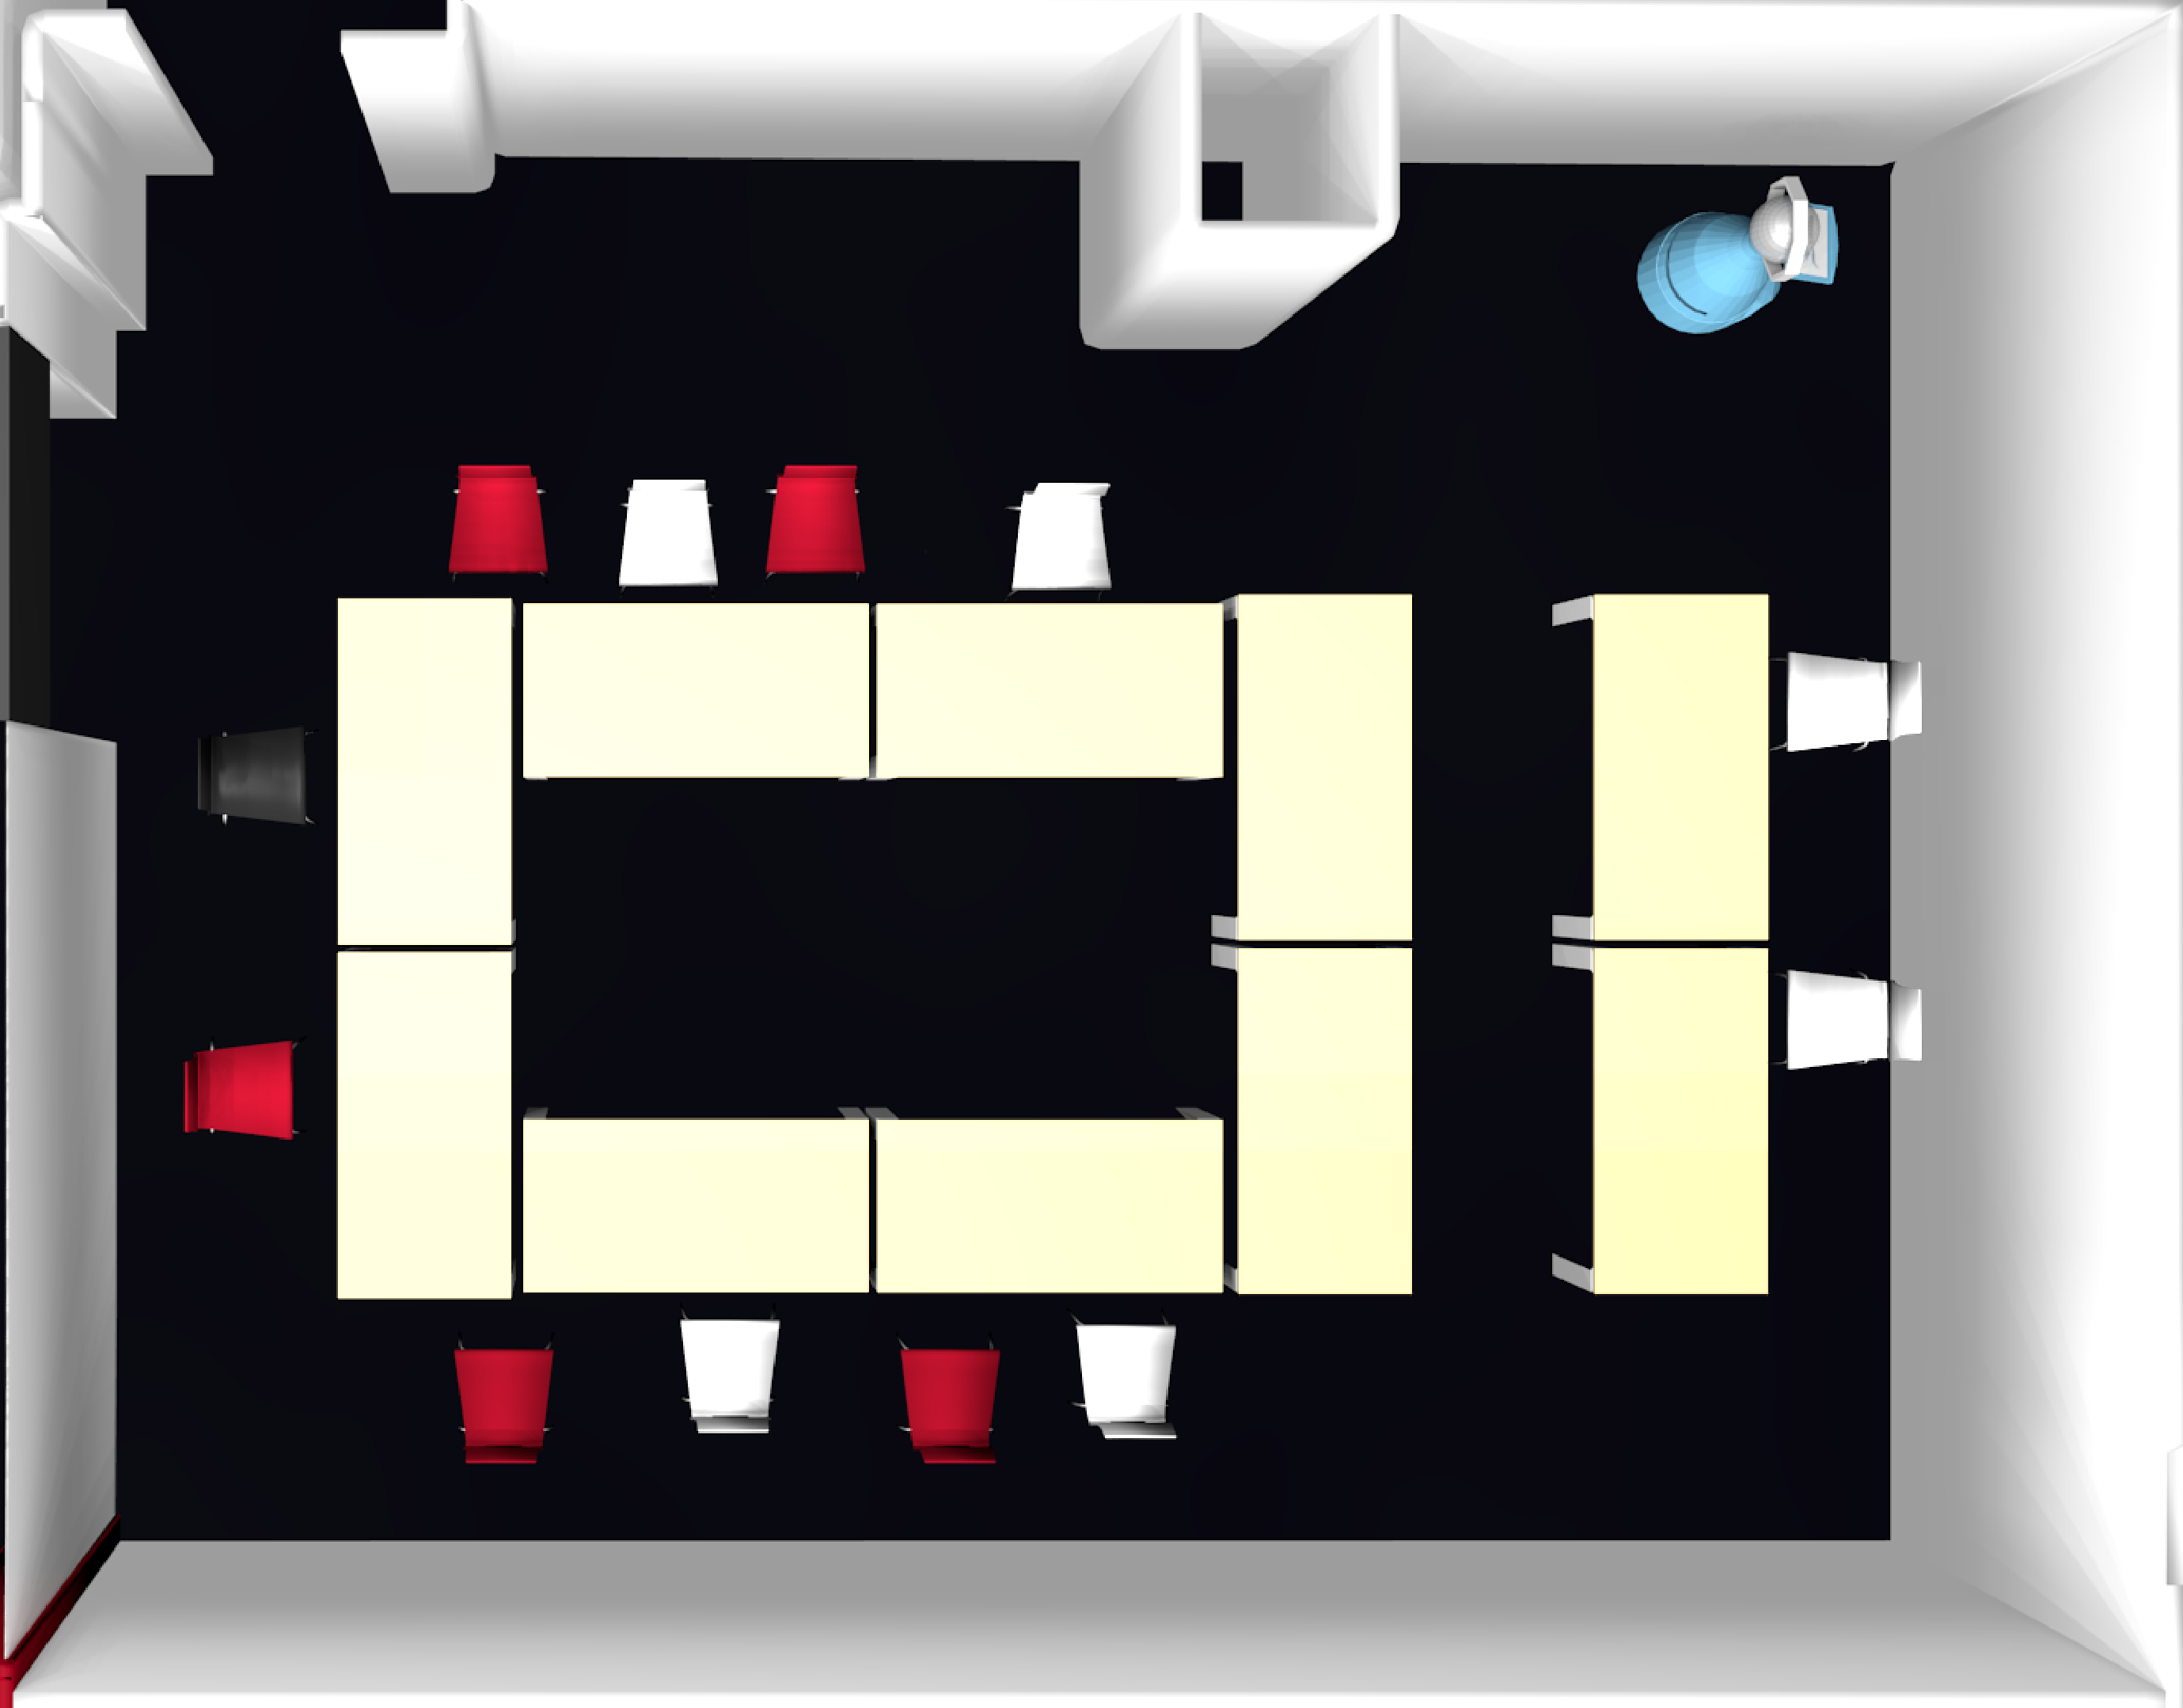
\includegraphics[width=\linewidth]{uol_bl_phase_3_small}
		\caption{One of the rooms in the (simulated) \texttt{uol\_bl} environment. The mobile robot, seen in the top-right, is presented the task of moving from its current location to a location in the main hall, outside the room.}
		\label{fig:uol_bl_tuning_1}
	\end{subfigure}
	\hfill
	\begin{subfigure}{0.475\textwidth}
		\centering
		\vspace{19.5pt}
		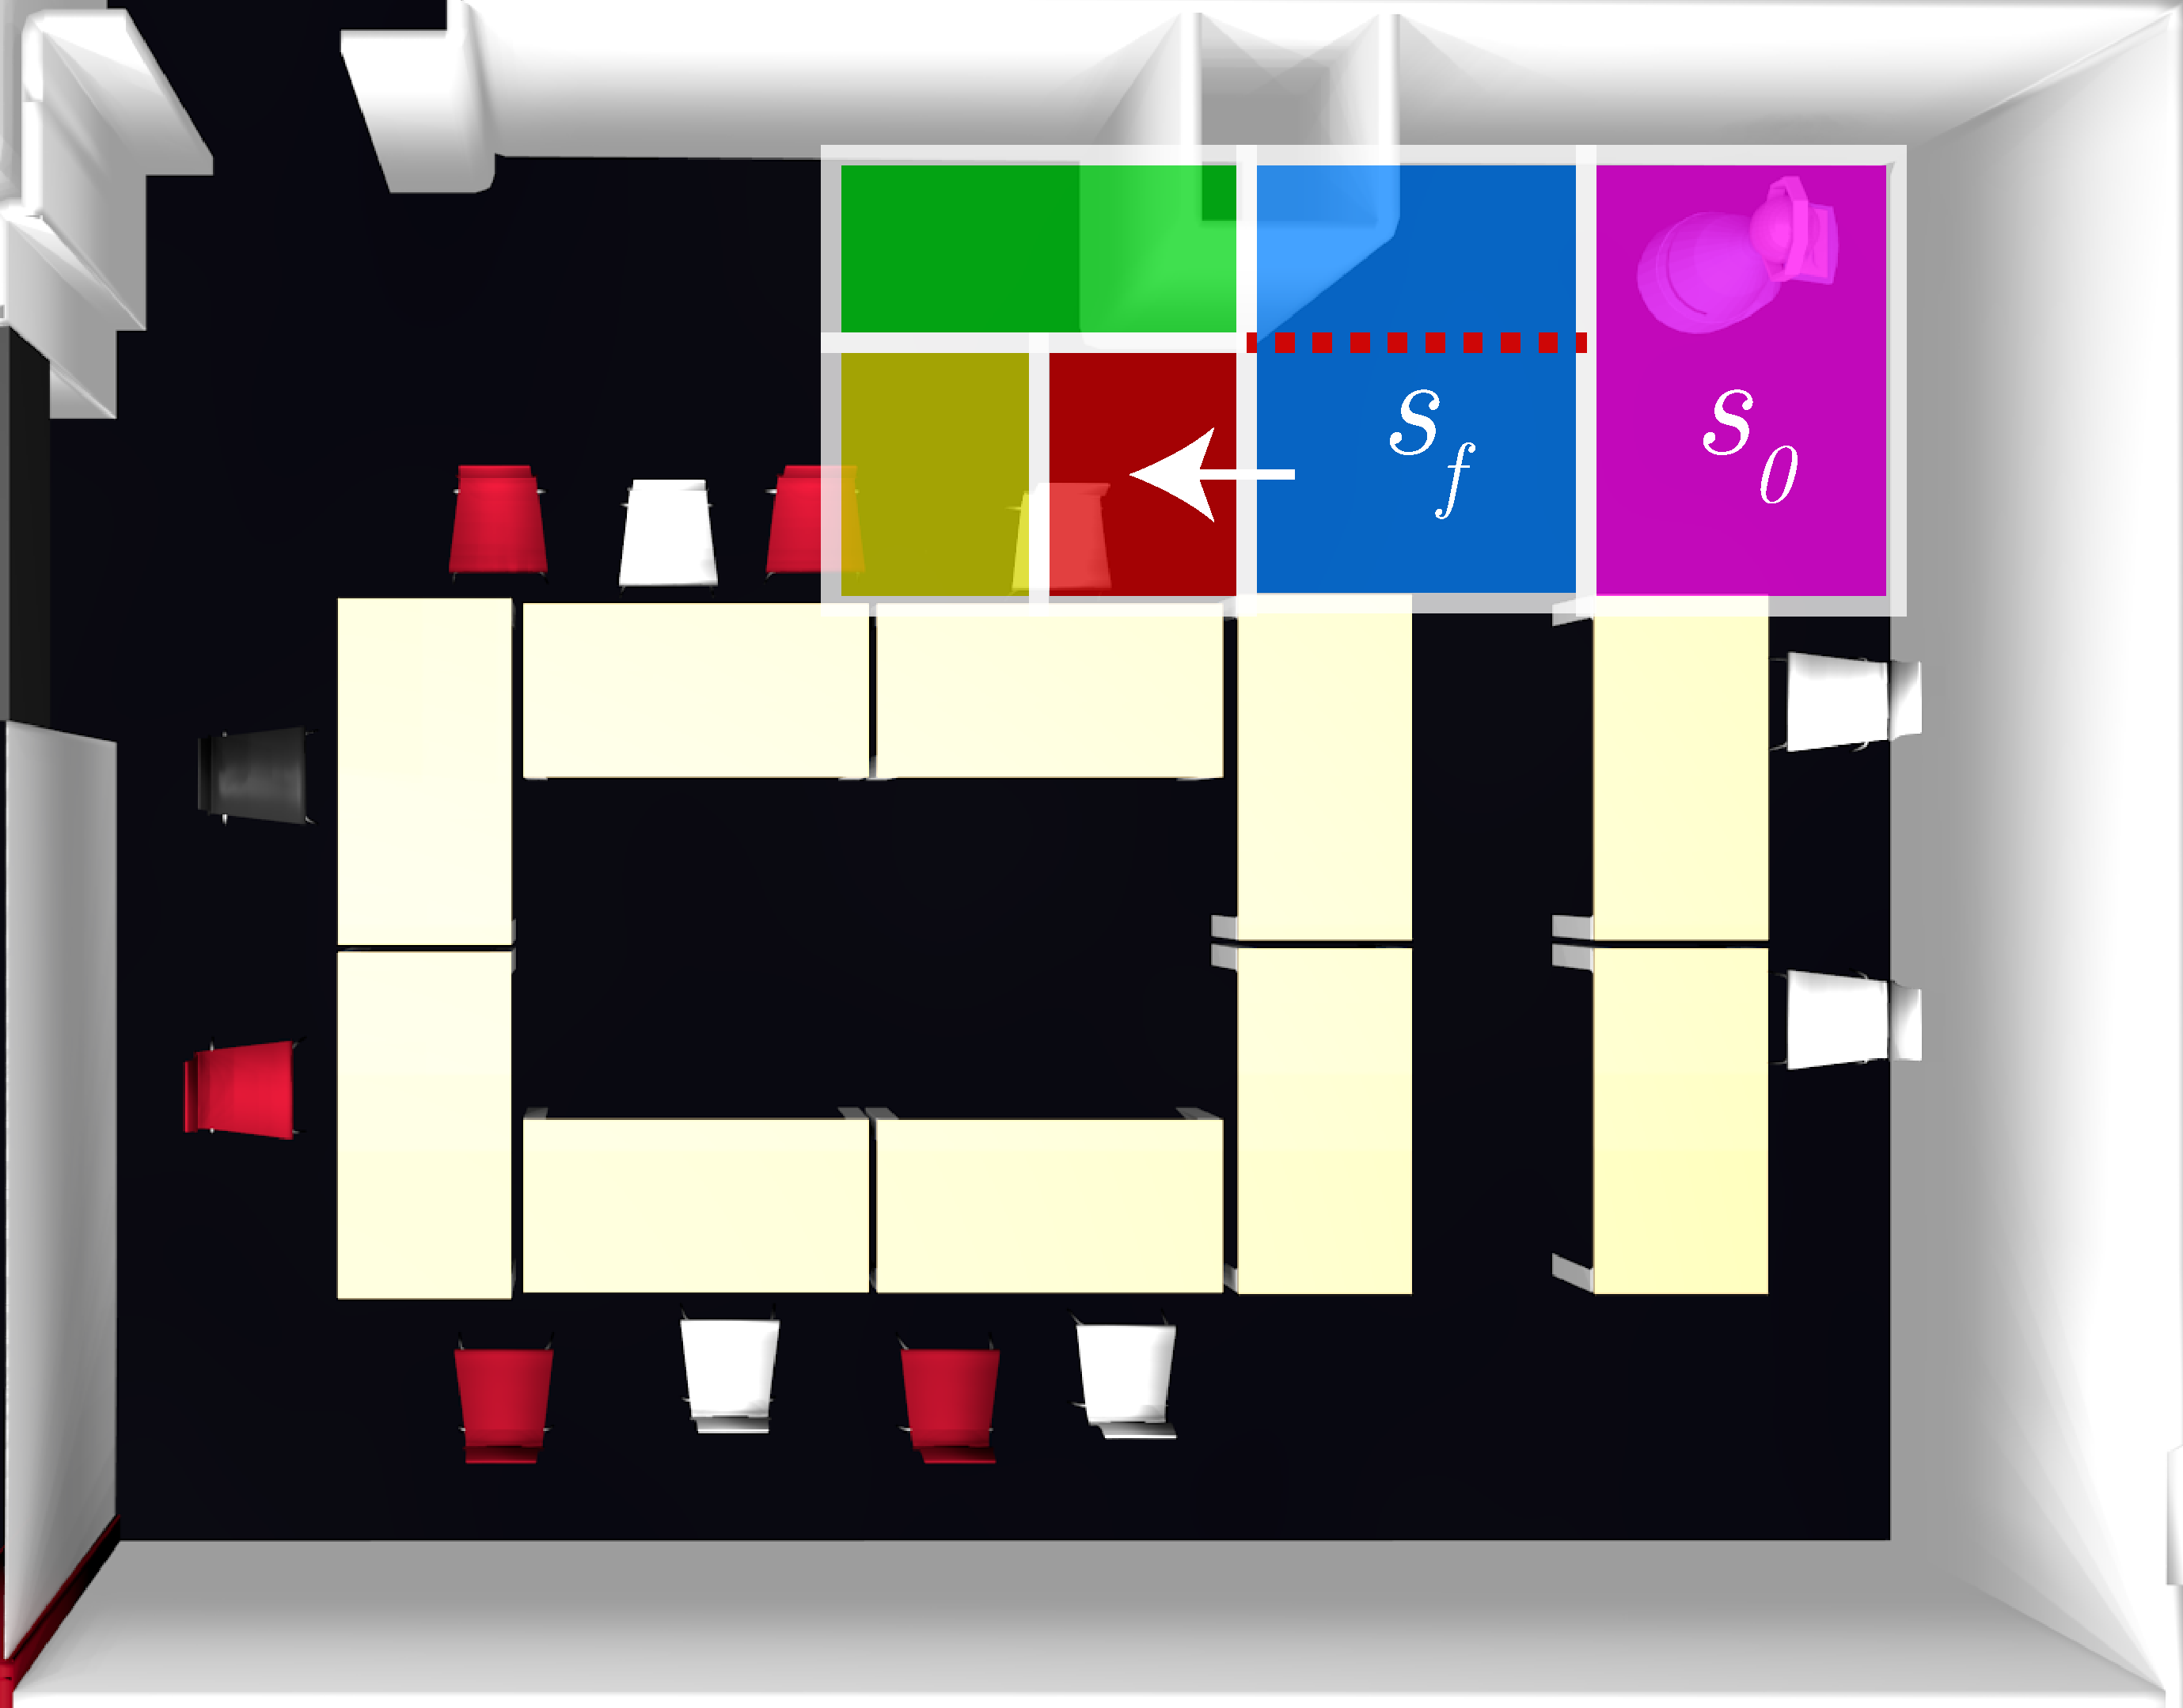
\includegraphics[width=\linewidth]{uol_bl_phase_3_2_smallv6}
		\caption{Illustration of the area of the earlier-learned state space of interest. The resolution for the part of the state space as shown is too low, particularly, considering the state $s_f$, which might cause the robot to get stuck. The third phase of the multi-phase framework therefore splits the state, as depicted by the dotted red line, based on new centroids.}
		\label{fig:uol_bl_tuning_2}
	\end{subfigure}
	\bigskip
	
	\caption{Illustration of the third phase of the multi-phase framework in a simulation of the \texttt{uol\_bl} environment. The phase starts off with the \acrshort{acr:mdp} model learned in the previous phase, and further fine-tunes this model after the robot gets stuck executing a new task.}
	\label{fig:uol_bl_tuning}
\end{figure}

Finally, we get back at the third phase of our multi-phase framework, in which the \acrshort{acr:mdp} $\mathcal{M}$ obtained in the previous phase is further fine-tuned, given a set of new tasks.
To investigate the expediency of this third phase, an implementation of the solution proposed in \autoref{alg:multi-phase-fine-tuning} has been made for the mobile robot navigation application.

Given a task to execute, the solution solves \acrshort{acr:mdp} $\mathcal{M}$ (with new initial state and reward function for this task) for a policy, which it uses to perform the task.
Then, if the controlled robot gets stuck in a state $s_f$ in its attempt to complete the task, it starts to gather new experience about the transitions possible from this state in a collection $E_\mathit{SIM}$.
Based on this new experience, the solution splits the state into a number of new (sub-)states through a clustering of the observations in $E_\mathit{SIM}$, and accordingly updates the transition probabilities based on the new data.
The updated \acrshort{acr:mdp} is then used to compute a new policy for the task, after which the agent tries to perform the task again.
If the agent gets stuck in the same state $s_f$ a clustering with higher resolution is applied to split the state.

For our implementation of this proof-of-concept solution, the mobile robot executes and gathers new experience in a simulation environment.
In gathering new experience, the mobile robot stores the observations (i.e., odometric readings) it makes and the state $s'$ it ends up in after executing an action $a$ from these observations.

To evaluate the approach, we take the \acrshort{acr:mdp} $\mathcal{M}$ learned in the second phase of our last experiment (i.e., see \autoref{fig:exp16}) for the \texttt{uol\_bl} environment.
Then, a new task is presented, which requires the robot to move from the corner of a room in the environment, as shown in \autoref{fig:uol_bl_tuning_1}, to a location in the main hall outside the room.
The problem, is that the resolution in the learned state space $\mathcal{S}$ of $\mathcal{M}$ for this area is too low, as shown in \autoref{fig:uol_bl_tuning_2}, caused by the limited execution traces gathered for this area in the set $E$ used for learning the model.
As a result, there is a considerable chance the robot gets stuck in the state labeled~$s_f \in \mathcal{S}$ from its starting location.

To take care of this, after the observation is made that he robot got stuck, the algorithm makes the robot gather new data about the transitions possible from the different locations within the state $s_f$ in which it got stuck.
Based on this data, the algorithm clusters the data to effectively split the state in two, well-nigh as shown in \autoref{fig:uol_bl_tuning_2}.
The resulting \acrshort{acr:mdp} with updated state space and transition probabilities then allows the mobile robot to successfully accomplish the task (i.e., by the computed policy suggesting to move south and west subsequently).

Although the algorithm works well for fixing small discrepancies like these in the model, caused by limited data about a certain area of the environment, it is not well suited for learning major parts of the model from the ground up.
For such scenarios, one is better off using existing \acrshort{acr:rl} solutions, such as continuous $Q$-learning or active learning approaches which use the learned \acrshort{acr:mdp} as a prior model (see \autoref{sec:active-learning}).
\chapter{Conclusions}
\label{ch:conclusions}

The goal of this thesis is to provide a foundation for an algorithmic technique for learning \acrfullpl{acr:mdp} for planning under uncertainty which maximize yielded performance given a dataset describing the dynamics of a system in need of automated control.
This chapter presents a summary of the presented work and the contributions made in \autoref{sec:summary} and revisits the identified research questions in \autoref{sec:revisiting-research-questions}.
Finally, this chapter concludes this thesis with recommendations and suggestions for future work in \autoref{sec:recommendations-future-work}.% and our concluding remarks in \autoref{sec:concluding-remarks}.

% 'Don't ignore RL, could be used together'
% Continuous-state?
% Partially Observable?

\section{Summary of Contributions}
\label{sec:summary}

Previous work in the field of probabilistic model learning for planning under uncertainty has already presented us with various algorithms for (offline) learning \acrfullpl{acr:mdp} from a dataset describing the dynamics of some system.
The state of the art however lacks an automated method of setting the hyperparameters of these learning algorithms so to best reflect the underlying system and maximize its performance in the execution of the tasks it is expected to perform.
To address this issue, we pose the adjustment of the parameters of such learning algorithms as an optimization task.
In this optimization task, the goal is to find the setting of the hyperparameters $\theta$ which maximizes the performance yielded by executing the plans or \textit{policies} derived from the learned \acrshort{acr:mdp}.

In this thesis, we present a solution (which we refer to as the \textit{\acrshort{acr:mdp} optimization framework}) that employs the \acrfull{acr:bo} framework for this optimization task, defining a probability distribution over functions which maps parameter settings $\theta$ to an assessment of the value $V_\mathcal{M}$ of a learned \acrshort{acr:mdp}.
Although algorithms that employ the \acrshort{acr:bo} framework for \acrshort{acr:sdm} problems do already exist, all of them are online \acrshortpl{acr:rl} approaches that do not utilize an available dataset prior to interacting with the real-world environment.
The model value $V_\mathcal{M}$ of an \acrshort{acr:mdp}, used as a relative performance measure in the optimization, is assessed based on computed value functions and simulations of the tasks the system is expected to perform.

Additionally, we extended our proposed solution by exploiting the lower cost of computing a value function in comparison to performing time-expensive simulations, to define our \textit{multi-phase optimization framework}.
That is, we define a first phase in which a \acrshort{acr:bo} is performed to maximize the average expected value for the \acrshort{acr:mdp} for a set of tasks to perform.
The posterior resulting from this phase is then used to steer the acquisition in a second optimization phase, in which the performance in simulations over a set of tasks is being optimized.

Then, finally, we present a solution to further fine-tune the parameters of the \acrshort{acr:mdp} resulting from this optimization.
This is done by increasing the resolution of the state space and updating the transition probabilities where necessary, e.g., when the agent gets stuck in a certain state.

An implementation of the aforementioned framework has been made for path planning in a mobile robot navigation domain, in which a robot needs to move from one location to another in an office environment.
A dataset of execution traces with odometric readings has been gathered based on which our implementation learns \acrshortpl{acr:mdp} by clustering the data into a state space, with the number of states defined by $\theta$.
The implementation thus optimizes for an \acrshort{acr:mdp} that can produce policies for a mobile robot offline, so that it can move from one location to another as fast as possible.

The results of the experiments show that our framework can effectively be used to obtain an \acrshort{acr:mdp} for the path planning of a mobile robot.
The first phase in the multi-phase framework shows out to be able to steer the acquisition in the second phase towards a global maximizer in some scenarios.
And finally, the proof-of-concept implementation of the last phase, can successfully be used to further fine-tune the parameters of a learned \acrshort{acr:mdp} when the mobile robot gets stuck in some state when presented with a new task.

% Discussion of the results
% Contributions made

\section{Revisiting the Research Questions}
\label{sec:revisiting-research-questions}

To answer the main research question of this thesis, the four research questions presented in \autoref{sec:research-questions} are revisited in this section.
First off, the following research question is mostly concerned with getting a good overview of the state of the art for learning \acrshortpl{acr:mdp} from a dataset:

\vspace{16pt}
\noindent%\fbox{\parbox{\textwidth}{
\textbf{Research Question 1.} Which learning algorithms exist that can be employed for learning \acrshortpl{acr:mdp} from data for systems involving uncertainty that require plans for automated control?
%}}
\vspace{0pt}

As seen in \autoref{sec:learning-markov-models}, one of the most straightforward methods can be deducted from methods for fitting Markov Chains, i.e. by maximum likelihood or Bayesian inference.
The difference is in the addition of actions, so that a transition probability matrix needs to be learned for each possible action, given some user-defined state space.
For various domains, such as that of mobile robot navigation, defining the state space may not be a trivial task, although there are approaches for this, such as $k$-Means clustering or (time-)state merging approaches, which are parameterized by the number of states.
Then, when one needs to learn partially observable models one needs to consider other approaches, as shown in \autoref{sec:learning-probabilistic-models} to account for emission probabilities as well.

\vspace{16pt}
\noindent%\fbox{\parbox{\textwidth}{
\textbf{Research Question 2.} How should a performance measure be defined which can be used to fairly compare the value of different \acrshortpl{acr:mdp}?
%}}
\vspace{12pt}

The value $V_\mathcal{M}$ of an \acrshort{acr:mdp} $\mathcal{M}$ should be defined in terms of how well the agent performs tasks based on the policies computed from the model.
Therefore, first of all, the performance can be estimated using the expected value in the initial state from the value function for multiple tasks.
However, as a model abstracts from the real world, using the value function to express model value is not always sufficient.
Therefore, a more accurate estimation can be made through simulations of the tasks the system is expected to perform, discounting the obtained reward based on the number of steps made.
Combining these estimations results in the expression shown in \autoref{eq:vm} in \autoref{sec:learning-step}, which can be used as a relative performance measure of different \acrshortpl{acr:mdp} for the same environments.

\vspace{16pt}
\noindent%\fbox{\parbox{\textwidth}{
\textbf{Research Question 3.} How can the parameter space of model learning algorithms cost-effectively be explored towards a global maximizer with only limited knowledge about the system under consideration?
%}}
\vspace{12pt}

We have seen that making an accurate assessment of the value of an \acrshort{acr:mdp} requires time-expensive simulations to be performed.
Therefore, it is important to limit the number of evaluations of a parameter setting for the used model learning algorithm, with \acrshort{acr:bo} emerging as an attractive framework for optimization.
As we have seen in our experiments, \acrshort{acr:bo} could effectively be employed to explore the parameter space with a limited number of evaluations.

\vspace{16pt}
\noindent%\fbox{\parbox{\textwidth}{
\textbf{Research Question 4.} How can the hierarchy of different abstraction levels be exploited to find a performance-maximizing \acrshort{acr:mdp} in a more cost-effective way?
%}}
\vspace{12pt}

This research question has been addressed by the multi-phase framework proposed in \autoref{sec:multi-phase-framework}.
In the first phase a \acrshort{acr:bo} for an \acrshort{acr:mdp} with the model value based solely on the value functions for the set of tasks over which to evaluate the performance.
The resulting posterior is then used in the second phase to steer the acquisition of the first few samples.
In our experiments we have seen that it is possible to use the first phase to successfully steer the optimization in the second phase towards a global maximizer.

% Revisiting the research questions

\section{Recommendations and Future Work}
\label{sec:recommendations-future-work}

As this thesis has only limited itself to learning and optimizing fully observable \acrshortpl{acr:mdp}, one direction for proposed future work is to explore the possibilities of optimizing for \acrshortpl{acr:pomdp}.
That is, we should acknowledge that our experiments make the simplifying assumption that the state is directly observable from odometric readings, while in practice this does not hold up and would require execution traces with other sensor readings.
This would require one to make use of other model learning algorithms, such as the \textit{Baum-Welch} algorithm and state merging algorithms seen in \autoref{sec:learning-probabilistic-models}.
Apart from this, another recommendation for future work would be to implement and test the solution on applications other than path planning for mobile robot navigation.
Further, one could consider to explore and investigate alternative global optimization algorithms (e.g., see \cite{bergstra2011algorithms}) to address the problem statement of this thesis.

\vspace{12pt}
\noindent\minibox[frame]{\textbf{Note:} This section will be updated and extended for the final version of the report.}

% Recommendation: POMDPs for Dialogue Management as seen in http://mi.eng.cam.ac.uk/~sjy/papers/ygtw13.pdf
% http://citeseerx.ist.psu.edu/viewdoc/download?doi=10.1.1.129.2652&rep=rep1&type=pdf
% Model checking, for instance refer again to lacerda2015 and refer to the routine in figure shown in earlier chapter


%% Use letters for the chapter numbers of the appendices.
\appendix

%\input{appendix-a}

% Acronyms and Glossary
\printglossary[type=\acronymtype] % makeindex main.acn -s main.ist -t main.alg -o main.acr
\addcontentsline{toc}{chapter}{Acronyms} % toc gives different font
%\printglossary

\bibliography{references}

\end{document}

% Using the order described here: http://academia.stackexchange.com/questions/5569/where-in-a-thesis-should-a-glossary-be-positioned

%TODO Check for consistent spelling, probably update glossary and check for use of dashes and change words to reach consistency

%TODO List of Figures?